\documentclass[a4paper,titlepage,openright,12pt]{report}
\usepackage{graphicx}    
\usepackage{color}
%\usepackage{epsfig}   
\usepackage[font=footnotesize]{subfig}
\usepackage{float}
\usepackage{fancyhdr}                              
\usepackage{makeidx}
\usepackage[nottoc,notlot,notlof]{tocbibind}     
\usepackage{supertabular}
\usepackage{array}              
\usepackage{setspace} 
\usepackage{enumerate}
\usepackage{rotating}
\usepackage{moreverb}
\usepackage{multirow}
\usepackage{amsmath}
\usepackage{amsthm}
\usepackage{amssymb}
\usepackage{captcont}
\usepackage{verbatim}
\usepackage{titlesec}
\usepackage{url}
\usepackage{hyperref}
\usepackage{lipsum}
\usepackage{tikz}
\usepackage{pgf-pie}
\usepackage{pgfplots}
\usepackage{array}
\usepackage{booktabs}
\usepackage{blindtext}
%\usepackage[utf8]{inputenc}
\usepackage{commath}
\usepackage{pbox}
\usepackage[toc,page]{appendix}
\newcolumntype{L}[1]{>{\raggedright\let\newline\\\arraybackslash\hspace{0pt}}m{#1}}
%\usepackage[algoruled]{algorithm2e}
%\usepackage[figure,algoruled]{algorithm2e}
%\usepackage[figure,boxruled]{algorithm2e}

%\newtheorem{theorem}{Theorem}
%\newtheorem{corollary}[theorem]{Corollary}
%\newtheorem{conjecture}[theorem]{Conjecture}
%\newtheorem{lemma}[theorem]{Lemma}
%\newtheorem{proposition}[theorem]{Proposition}
%\newtheorem{definition}[theorem]{Definition}
%\newtheorem{Example}[theorem]{Example}
%\newtheorem{axiom}{Axiom}
%\newtheorem{remark}{Remark}
%\newtheorem{exercise}{Exercise}[section]
%\newtheorem{fact}[theorem]{Fact}
%\newtheorem{property}[theorem]{Property}
\setlength{\parindent}{0pt}%for paragraph spacing
\setlength{\parskip}{1ex plus 0.5ex minus 0.2ex}
\setlength{\textheight}{8.5in}
\pagestyle{fancy}
% with this we ensure that the chapter and section
% headings are in lowercase.
%\renewcommand{\bibname}{References}
\renewcommand{\chaptermark}[1]{\markboth{#1}{}}
\renewcommand{\sectionmark}[1]{\markright{\thesection\ #1}}
\fancyhf{} % delete current setting for header and footer
\fancyhead[LE,RO]{\bfseries\thepage}
\fancyhead[LO]{\bfseries\rightmark}
\fancyhead[RE]{\bfseries\leftmark}
%\rfoot{\bfseries\thepage}
\cfoot{\em $\copyright$ 2015-16, Indian Institute of Technology Delhi}
\renewcommand{\headrulewidth}{0.5pt}
\renewcommand{\footrulewidth}{0.5pt}
\addtolength{\headheight}{2.5pt} % make space for the rule

\fancypagestyle{plain}{%
\fancyhead{} % get rid of headers on plain pages
\fancyfoot{}
%\rfoot{\bfseries\thepage}
\cfoot{\em $\copyright$ 2015-16, Indian Institute of Technology Delhi}
\renewcommand{\headrulewidth}{0pt} % and the line
}

%% The smart version of cleardouble page.
\let\origdoublepage\cleardoublepage
\newcommand{\clearemptydoublepage}{%
  \clearpage
  {\pagestyle{empty}\origdoublepage}%
}

\let\cleardoublepage\clearemptydoublepage


\date{}


\addtolength{\oddsidemargin}{30pt}
\addtolength{\evensidemargin}{-40pt}

\titlespacing*{\chapter}{0pt}{-50pt}{20pt}
\titleformat{\chapter}[display]{\normalfont\huge\bfseries}{\chaptertitlename\ \thechapter}{20pt}{\Huge}
% \DeclareGraphicsExtensions{.pdf,.png,.jpg,.ps}
\floatstyle{boxed} 
\restylefloat{figure}
\setcounter{lofdepth}{2}
\setcounter{lotdepth}{2}

\newtheorem{claim}{Claim}[section]
\newtheorem{theorem}{Theorem}[section]
\newtheorem{defn}{Definition}[section]
\newtheorem{fact}{Fact}[section]

\graphicspath{{./Figures/}}
\begin{document}

%\begin{comment}
% Begin title page
\begin{titlepage}
\begin{center}

\LARGE{\textsf{\bfseries DATA ANALYSIS OF COMMODITY PRICES}}\\
\vspace{20pt}
\normalsize
\emph{A thesis submitted in partial fulfillment} \\
\emph{of the requirements for the degree of} \\
\vspace{20pt}
\bfseries MASTER OF TECHNOLOGY \\
\vspace{20pt}
\emph {in}\\
\vspace{20pt}
\bfseries Computer Science \& Engineering \\
\vspace{20pt}
\emph {by}\\
\vspace{20pt}
\Large{\textsf{\bfseries KAPIL THAKKAR}} \\
{\normalsize \textsf{\bfseries Entry No. 2014MCS2124}}\\
\ \\
%\ \\
{\normalsize \emph {Under the guidance of}}
\ \\
\Large{\textsf{\bfseries Dr. Aaditeshwar Seth}} \\
\ \\
\vspace{30pt}
%\begin{center}

\includegraphics[scale=0.2]{iit_logo.pdf} \\
\vspace{10pt}
%\end{center}
\large{\textsc{Department of Computer Science and Engineering,\\
Indian Institute of Technology Delhi.\\ Jan 2016.}}
\end{center}
\end{titlepage}

%\newpage
%\cleardoublepage
\onehalfspacing
\thispagestyle{empty}

\normalfont
\begin{center}
\LARGE{ Certificate} 
\end{center}

\vspace{0.5in}

This is to certify that the thesis titled {\bfseries TIME SERIES ANALYSIS} being submitted by
{\bfseries RESHMA KUMARI} for the award of {\bfseries Master of Technology} in {\bfseries Computer Science \& Engineering} is a record of bonafide work carried out by him under my guidance and supervision at the {\bfseries Department of Computer Science \& Engineering}. The work presented in this thesis has not been submitted elsewhere either in part or full, for the award of any other degree or diploma.

\vspace{1.5in}


{\bfseries Dr. Aaditeshwar Seth} \\
{\bfseries Department of Computer Science and Engineering} \\
{\bfseries Indian Institute of Technology, Delhi}\\ 

\thispagestyle{empty}
%\begin{center}
\LARGE{Acknowledgments} 
\end{center}

\vspace{0.5in}

%Replace \lipsum with your acknowledgement
I would like to express my heartiest gratitude to our supervisors Dr. Aaditeshwar Seth for guiding this work with utmost interest,
patience, care and scientific rigor. We thank him for setting high standards, giving us freedom to explore multiple facets of the problem and teaching us value of analytical thinking and hard work.

I would also like to thank Dipanjan Chakraborty who have helped a great deal by providing technical guidance and support whenever needed. 

\vspace{1.5in}

{\bfseries KAPIL THAKKAR}

\thispagestyle{empty}


% \setcounter{page}{1}
% \pagenumbering{roman}
\thispagestyle{empty}


\begin{abstract}

This document explains the methods and corresponding function written for Anomaly detection Library to detect anomaly in multiple time series. All corresonding files can be found in ``library'' folder. We have performed analysis on Onion data considering its Retail Price, Wholesale Price and Arrival data. File used to perform analysis and studying various results is ``library/fullAnalysis.py''. To study local and national anomalies file used is ``library/fullAnalysisUpdated.py''. ``fullAnalysis.py'' file contains required comments to understand how analysis is performed.

\end{abstract}

      


\thispagestyle{empty}
\begin{center}
\LARGE{Acknowledgments} 
\end{center}

\vspace{0.5in}

%Replace \lipsum with your acknowledgement
I would like to express my heartiest gratitude to our supervisors Dr. Aaditeshwar Seth for guiding this work with utmost interest,
patience, care and scientific rigor. We thank him for setting high standards, giving us freedom to explore multiple facets of the problem and teaching us value of analytical thinking and hard work.

I would also like to thank Dipanjan Chakraborty who have helped a great deal by providing technical guidance and support whenever needed. 

\vspace{1.5in}

{\bfseries KAPIL THAKKAR}


\thispagestyle{empty}
\tableofcontents

\thispagestyle{empty}

\listoffigures

\listoftables
%\end{comment}

\thispagestyle{empty}
\cleardoublepage
\onehalfspacing
%%%%%%%%%%%%%%%%%%%%%%%%%%%%%%%%%%%%%%%%%%%%%%%%%%%%%%%%%%%%
 
\setcounter{page}{1}
\pagenumbering{arabic}

%You may have as many chapters as you please. This is just for reference.

\chapter{Introduction}


\section{Motivation}

Supply demand imbalance, natural calamities etc. may not always be the reason behind the rise in the price of a commodity. ​It may be a consequence of artificial supply deficit planned intelligently by traders’ nexus for profiteering through manipulation of supply of commodity and hence indirectly controlling their prices. ​Our attempt is to locate such hikes in prices which seem suspicious (we call them anomalies).​ To detect and analyse the characteristics of anomalies in the prices of commodities. Currently we have considered the case of onion and based on that we have developed one library which has multiple functions to detect anomalies in the time series.


\section{Objective}

Our objective is that we need to highlight anomalies which may be an indicator of illegal market manipulation act by traders nexus in the provided time series. For this purpose we need to create library with some set of functionalities to detect anomalies in the give input time series. Anomalies will be based on the hypothesis stated by the user. For different scenarios user can pass appropriate parameters to functions and functions will report anomalies to user based on that.


\section{Relavence of Project}

Anomaly detection techniques help to explore situations which might be different from the expected behavior and could reveal interesting facts. It is used many areas which are explained in detail in next chapter. The project aims to raise potential red flags for days which are suspect of illicit market manipulation activities by set of traders. This type of monitoring system may help people monitor and hence control these illicit market manipulations better.
For example, unnecessary hike in the prices may be due to wrong government policies, loopholes in the supply chain of commodity, intention of profiteering by traders etc. So our project will help journalist or end user interested in detecting such abnormal behavior.


\chapter{Literature Survey}

%Replace \lipsum with text.
% You may have as many sections as you please. This is just for reference.

\section{What is Anomaly Detection?}

According to wikipedia, anomaly detection (or outliers detection) is the identification of items, events or observations which do not conform to an expected pattern or other items in a dataset.

Here, our major focus is on detecting anomalies in the time series data. Time series usually considers data about price of some commodity, production, sell, etc. Usually, these time series follow some normal pattern. Some time series may be independent or behavior of some may depend on other time series. It may also consist of seasonality and trend along with some noise. So, considering all these factors our aim will be to detect some points on time line during which these time series does not follow a normal pattern.

Reasons for presence of anomaly may be different depending upon the type of time series. We have considered time series of onion data as a use case. In case of onion presence of anomalies could be because of unseasonal rainfall, hoarding, price manipulation by traders' nexus, effect of import/export of onions, variation in production, etc. Being a seasonal crop, some part of onions are stored during harvest, so that demand can be met in lean season. But some traders hoard huge stocks for the purpose of profiteering. According to wikipedia, in economics, hoarding is the practice of obtaining and holding scarce resources, possibly so that they can be sold later to customers for more profit. So during this time also, we are able to see anomalies.


\section{Onion Case}


Onion is a staple ingredient for almost every Indian kitchen and hence its demand is almost constant throughout the year but not the supply. In order to supply onions throughout the year, they are stored during harvest and released into markets in lean seasons. Its importance can be well estimated by the fact that it is one among few essential commodities and often rise in its price has resulted into downfall of state and central government.

One major tragedy in onion market occurred in end of year 2010. The prices of the onion increased so much that it was out of reach from poor people. There was a study conducted by the CCI (Competitive Commission of India) for this case and they created report on that \cite{CCI}. In this \cite{CCI}, they tried to find out the reasons behind this scenario. They came with the following things in their study:

\begin{itemize}

\item Large wholesalers/traders mainly operates in metropolitan city markets and large number of farmers dispose their bulk of produce in nearby markets because of absence of storage facility, immediate cash need for loans, family expenses, purchase of inputs of next season, etc.

\item Concentration of large storage capacities with traders,Vertical Integration of various market functions by onion traders(one
name, many roles), Existence of established traders and barrier to new entry

\item On December 23 of 2010, The Times of India published in an article that on Tuesday alone, wholesale traders in Delhi bought onion at about Rs.34 per kg while it was sold in retail at Rs. 80 per kg, the margin of Rs. 46 per kg or 135 \%.

\item In the weeks of November and December, wholesale price remains high, so retailers do not get much profit, but even after that when wholesale price go down, retailers particularly in metro cities, show strong rigidity in holding price and earn margin from 60 to 110 \%. This clearly shows that along with traders, retailers also exploit the situation of crisis for their own benefits.

\item If we take this forward, then government policies also had a great role in the December 2010 high price episode (export of 1.33 lakh tones onion in October 2010).

\end{itemize}

So if we consider its overall picture, then there was unseasonal rainfall in the month of September and October 2010, but after that also government policy regarding export of onion was unexplainable. The news article published in Times of India also questions why there is so much difference in the wholesale and retail price of onions. Study also suggests that all the traders operating in the market have experience of many years (20 years on an average) and this is sort of family business for them. Due to limited entries, there is also barrier for new traders in entering to the market. So no new person enters and because of existing traders monopoly, they operate in the market together by forming the nexus. So many times they can alter the prices in many regions so that farmer has to pay money they decide. Traders have monopoly in onion markets and due that prices do not follow normal behavior of demand-supply and goes out of the way.



\section{ Other Cases}

\subsection{Sugarcane Case}

This \cite{sugarcane} study on sugarcane shows the connections between Politicians and Sugar Mills in Maharashtra and explains how such connection may benefit to firms and politicians. Sugar mills are cooperatives and regions are formed according to mills present. Each sugarcane farmer has to sell his produce to the mill present in his region, he can not sell it to some other mill. Each mill pays its farmers a single price per metric tonne of cane every year, based on weight (not on the quality).

This study investigates how price of the sugarcane, paid to farmers, changes in the election year. Usually, chairman of the sugar mills are politicians who stands in election. They need funding for elections, so here author explains how sugarcane mills and election funding may be related. And if some chair person wins the election then what is effect on prices offered to farmers. Some findings are:

\begin{itemize}

\item Prices are lowered by about Rs. 20 a ton in politically controlled mills during election years

\item The results were robust to including rainfall and mill capacity as controls, as well as including mill-specific outcomes such as the recovery rate - sugar produced per unit cane, a measure of productivity - as well as various other mill level shocks such as mill breakdowns and cane shortages

\item Price fall may be due to mill closure, i.e. mill is not operating for profitably, but politicians has kept mill open as a way to gain votes. But analysis shows that mill closure is not affected by political control

\item Paying farmers Rs. 20 per ton less for their cane amounts to a total of Rs. 6 million

\item Mills whose chairmen won national elections pay Rs. 80 per ton more in the year after elections

\item Author finds that when the party affiliated with the mill chairmen is in power in Maharashtra, the mill pays Rs. 23 more in cane price and also Chairmen who win national elections seem to be able to keep their mills open far more successfully than chairmen who lose

\end{itemize}

So here author has strong belief that all facts indicates that funding for election campaign comes from these sugarcane mills if mill is  politically controlled. Reason why farmers supports this may be that, with average probability 1/3rd of winning election, on an average farmer gets Rs. 27 on their principal of Rs. 20, so still in profit. The overall effect on farmer welfare is difficult to determine. On average, cane prices and recovery rates in politically connected mills are no different than those in non-politically connected mills, and the levels of public goods are no different either.

So this example explains how time series may go out of their normal behavior though there is no supply-demand crisis or any other case.

\subsection{Builder-Politician Case}

This \cite{kapur2011quid} study shows in developing countries like India, where elections are costly and accountability mechanisms are poor, politicians often turn to private firms for illicit election finance. Land is one of the highly regularized sector in India which provides discretionary power in the hands of state(indirectly in the hands of politicians). It is easy for politicians to accumulate resources than to hide them. To hide these assets from scrutiny politicians often use real estates as medium because of its features which are absorptive capacity,liquid asset and Contract enforcement.
As elections approach, however, builders are often compelled to provide politicians with money with which to contest elections; the mechanism can be a simple under-the-table transfer or an in-kind contribution. Although builders have to transfer funds back to politicians around elections, the transaction brings long-term benefits in terms of future goodwill. Based on this author have quoted following hypothesis:

\begin{itemize}

\item Cement consumption should exhibit a significant contraction during the month of the state election.Because builders are a leading source of election finance, one would expect activity in the sector to slow down during the month-long campaign period prior to Election Day.

\item Contraction in cement consumption will be significant in national elections, though of a smaller magnitude than in state-level elections

\item The magnitude of the contraction in cement consumption to be larger for dual elections than if only a state or national election is being held.

\item cement consumption should exhibit a larger contraction in urban versus rural states.

\item The contraction in cement consumption should be comparatively larger in more competitive elections

\end{itemize}
 
 The paper was able to bring the quid pro quo relation between builders and politicians quantitatively.


\chapter{Study of Onion Data: Collection and Analysis}


\section{System}

For now, we are only working over onion data. We have three actors in model: Farmers who are producers of onion, traders who are collectively responsible for supply of onions across country and consumers who purchase onions.

\begin{figure}[h]
\begin{center}    
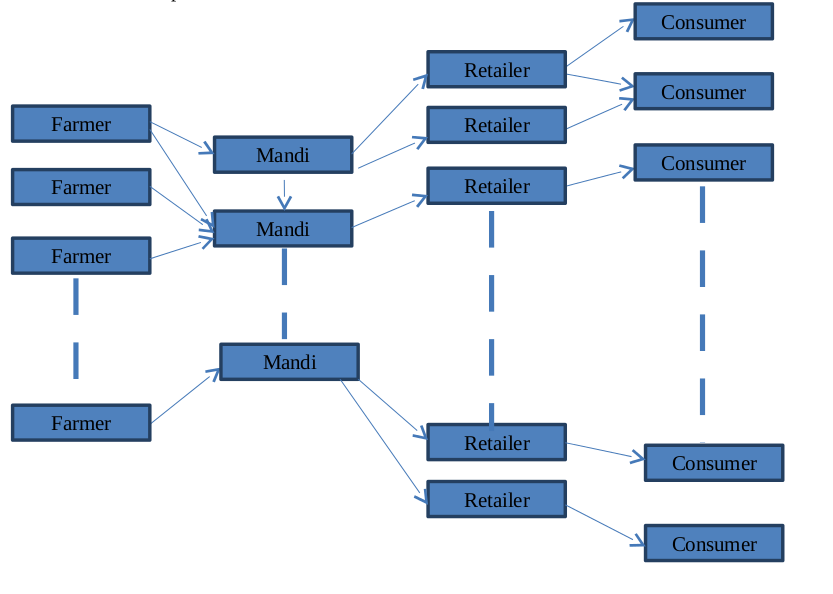
\includegraphics[scale=0.4]{3_1}
\caption{Normal Supply Chain}
\label{fig:Normal Supply Chain}
\end{center}
\end{figure}

Farmers sell their produce to traders in nearest mandi offering better price. These traders sell these commodities to traders in other mandis or to retailers. Consumers purchase commodities for consumption from one of the retail stores. This way commodity reaches consumers from farmers following a huge chain of traders and retailers.

Under APMC act, mandis were established at different places across country so that farmers can sell their produce directly in mandi and get good returns (wholesale price). There are around 1500 mandis located in different places across country which log their daily arrival of onion, minimum, maximum, modal selling price per quintal of onion data to AGMARKNET. Retailers purchase from these mandis and sell to end customers at retail price. There are around 70+ centres across country which maintains retail price of onion on Ministry of consumer affairs website.

\section{Data we have}

We have following data:

\begin{enumerate}

\item Daily wholesale price of onion for 1514 mandis
\item Daily arrival of onion information for 1514 mandis
\item Daily retail price of onion for 76 centres
\item Dates and location for hoarding reports from news articles
\item Longitude and latitude of mandis and centres

\end{enumerate}

Onion Data was collected from the the government websites,\cite{agmarknet} for arrival and wholesale price data and \cite{retailpricecollection} (Department of Consumer Affairs) for retail price data. Crawlers were written to collect the data from these datewise for the period of approximately 9.5 years, starting from Jan 2006 to Jun 2015. More data can be added simply by running crawlers again.


\section{Normal market behavior}

\begin{enumerate}

\item Wholesale price is inversely proportional to arrival of commodity –higher production of crop will lead to more and more crop hitting market for sell. Hence more arrival which will result in surplus supply leading to drop in wholesale prices.

\item  Retail price is directly proportional to wholesale price – commodities reach customers through a long chain of traders and retailers, adding value at every stage of chain. So, retail price at which customers purchase commodities are more than wholesale.

\end{enumerate}

Any divergence from these characteristics of normal market leads to suspicious price hike situations/anomalies.


\section{What are the reasons for anomaly?}

Primarily there are 3 main reasons of anomaly.

\begin{enumerate}

\item \textbf{Government Policies:} When the production is low in the country, still government allows the export of onion in large amount, or supports it by keeping low minimum price then the prices can rise up drastically.

\item \textbf{Unseasonal Rainfall:} Due to insufficient, heavy or unseasonal rainfall, onion crop may get affected and the produce is low and wholesale price may rise up. But, this reason still is validating that wholesale price is inversely proportional to arrival, it may be just prices will be little higher than what was supposed to be.

\item \textbf{Hoarding:} When traders/wholesalers store the onion and does not release the stock in the market in the expectation of the good prices in the future, it will create the artificial deficit in the market and will shoot up the onion prices in the retail market due to low arrival in the retail market. The reason people do this is to expect the higher prices in the time of low production or may be for security. For example, if it is expected that in some year the rainfall is not good, then people may predict  production to be low in the future and so they will start storing onion so that they can gain more profit. It will also create deficit in the market and price will go up.

\end{enumerate}

So our study will focus on detection of anomalies in data and if possible comment on the possible reason for the anomaly.

\section{Mapping of wholesale price to retail price}

Voronoi Diagram is used to map every mandi to nearest possible centre. The centres with retail data were considered fixed points and country was divided into 76 regions. All the mandis falling in that region are mapped to the respective centre.


\begin{figure}[h]
\begin{center}    
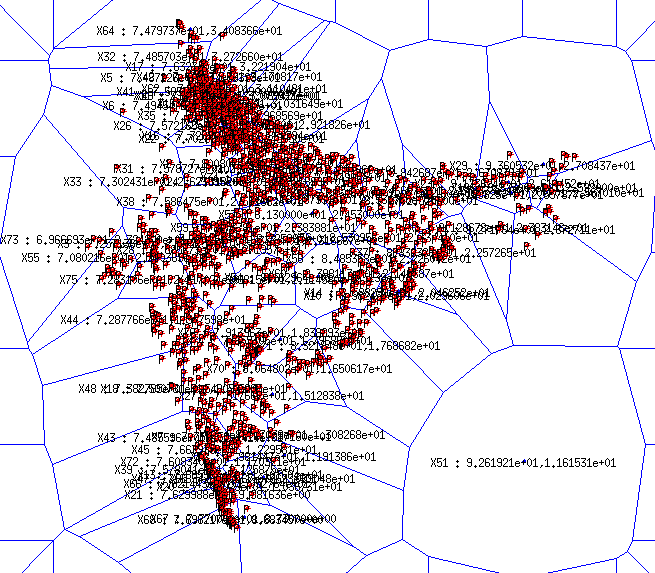
\includegraphics[scale=0.7]{3_2}
\caption{Voronoi Diagram}
\label{fig:Voronoi Diagram}
\end{center}
\end{figure}


After all the mandis are mapped to their nearest centre, wholesale and arrival at every centre is computed. Wholesale price at centre is average of modal price of all mandis in its region and arrival was computed as the sum of the arrival at the mandis in its region. While calculating the wholesale price, the distance between centre and the mandi was not considered.

Corresponding to every date and location of hoarding news report, values like current year arrival, last year arrival, Percentage difference in wholesale- retail etc. were computed. Following table resulted from these computations.


\section{How to Define Anomaly?}

To answer this question, we went through the series of the news articles when the hoarding is in the news. Then looking over those articles, we try to see that why they are reporting in news, what happened so that people are giving it name of hoarding and how reporters are making conclusion that it may be the class of the hoarding.

\subsection{Summary Of News Atricles}


First such incident was reported in the 1998. The article \cite{Redif57:online} dated on 21 st September 1999 states as follows:

\textit{ “Onions were retailed at Rs 6 a kilo two weeks back. Today, the price was almost 100 per cent up, hovering in the Rs 10-12 band in different parts of the country.” }

So this article is comparing the retail price of today with the price before 2 weeks. The rise upto 100\% is what has come to notice. Also article says that,

\textit{“There is talk in the market that the government is likely to lift the ban on onion exports. Apparently, some traders are resorting to hoarding in anticipation of demand from markets abroad.”}

As stated previously also, government policy also plays a major role in this. After that Onion was in news in 2010. NDTV \cite{Whyo17:online}, TOI \cite{Theg44:online} and many more reported the incident. In 2010, unseasonal rainfall and the government policy on export price were also the reason for hike in the price. The report dated Dec 23, 2010, TOI states the follows (in Delhi):

\textit{“On Tuesday alone, wholesale traders in Delhi bought onions at about Rs 34 per kg while it was sold in retail at Rs 80 per kg. That's a margin of Rs 46 per kg or 135\%!” }

Here, they have compared the difference between the wholesale price and the retail price. The margin of 135\% is reported. When we looked into data we have, we got the following results for Dec, 2010. (See figures \ref{fig:DelhiDec2010} and \ref{fig:DelhiDec2010Relativedifference})

\begin{figure}[h]
\begin{center}    
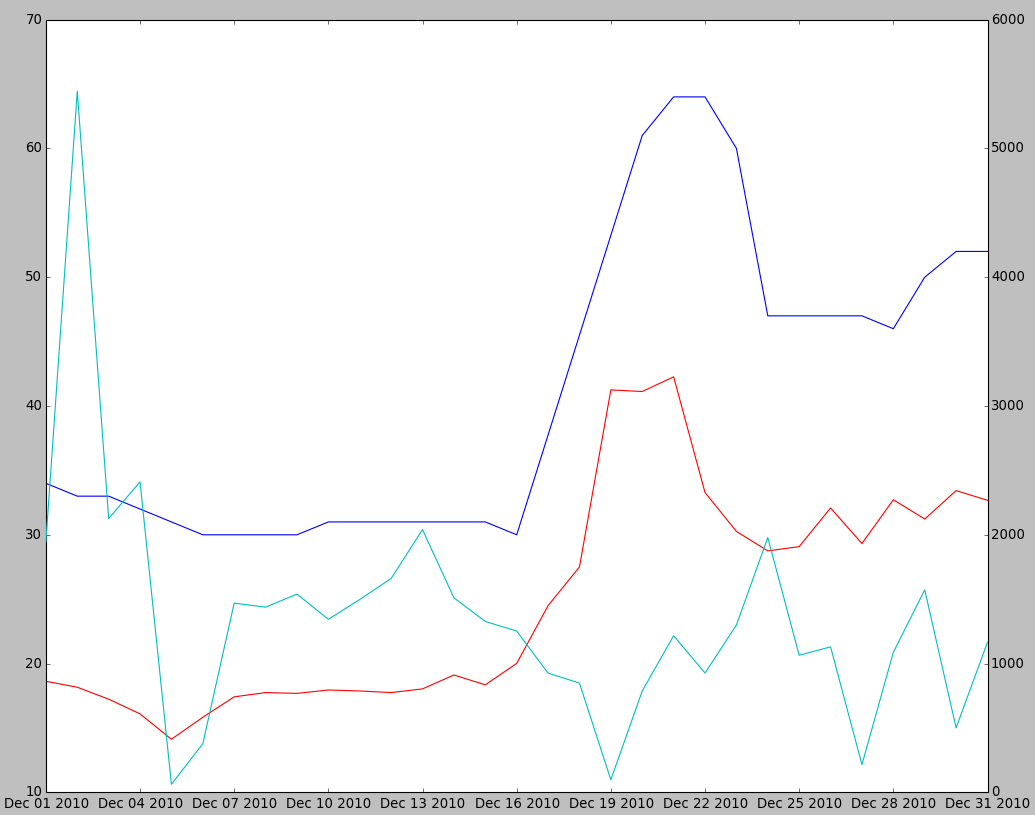
\includegraphics[scale=0.3]{2010_dec_delhi}
\caption{Delhi, Dec 2010. (Blue - Retail price, Red - Wholesale Price, Cyan - Arrival)}
\label{fig:DelhiDec2010}
\end{center}
\end{figure}

\begin{figure}[h]
\begin{center}    
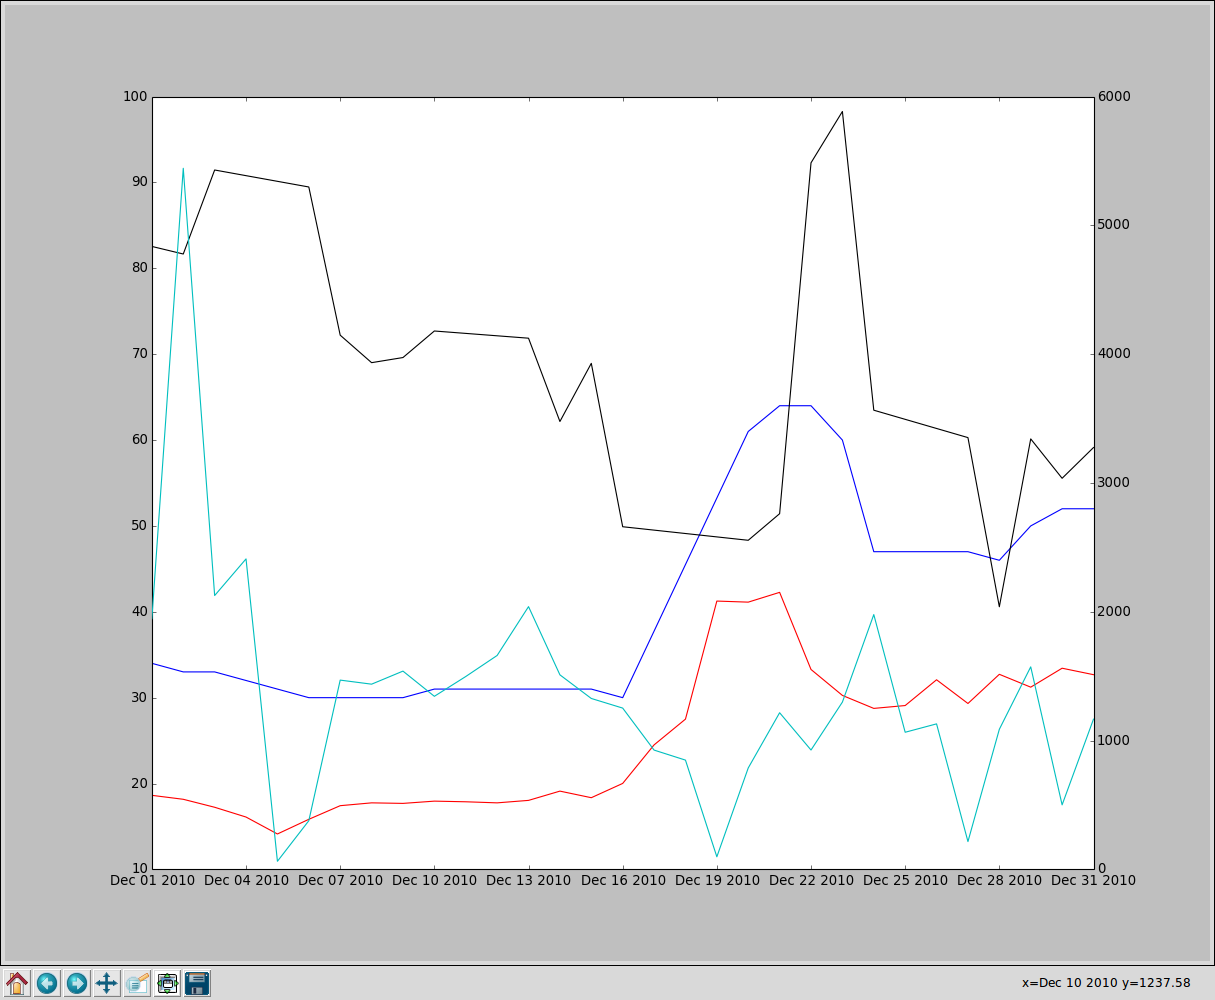
\includegraphics[scale=0.3]{2010_dec_delhi_with_relative_diff}
\caption{Delhi, Dec 2010. (Blue - Retail price, Red - Wholesale Price, Cyan - Arrival,Black - Relative difference \%)}
\label{fig:DelhiDec2010Relativedifference}
\end{center}
\end{figure}

So, as per our data, the maximum price difference observed was of \~ 100\% . Note that the retail prices we have is the minimum price observed in the market.

NDTV on Dec 22, 2010 reported the following (NASIK):

\textit{ "The average purchase rate of a trader here is about Rs. 3,000, but they go to the cities and claim it's nearly Rs. 8,000 and that's how the rates go up. It's all the fault of the traders. They loot the people," said Sangdeorao Holkar, Director, National Agricultural Cooperative Marketing Federation of India.}

Here also, as we see they have mentioned price difference between retail and wholesale in the market. It is approximately \~166\%.

Report also adds the following:

\textit{“The government, on a back foot, banned exports last evening. In less than 24 hours, prices in Lasalgaon crashed by 25 per cent.}\\
\begin{center}
\textit{Navi Mumbai: Wholesale price } \\
\textit{Tuesday: Rs. 60 per kg }\\
\textit{Wednesday: Rs. 45 per kg }\\
\end{center}
\textit{And this is finally what the consumer in Mumbai is paying:}\\
\begin{center}
\textit{Mumbai: Retail price}\\
\textit{Tuesday: Rs. 60 to Rs. 70 per kg}\\
\textit{Wednesday: Rs. 60 to Rs. 70 per kg” }\\
\end{center}
So as we can see, there is significant drop in the wholesale price, but no drop in the retail price, so that has been reported. Also difference in the hike in retail price, from 40 to 60 was reported in on week. What our data says:

\begin{figure}[h]
\begin{center}    
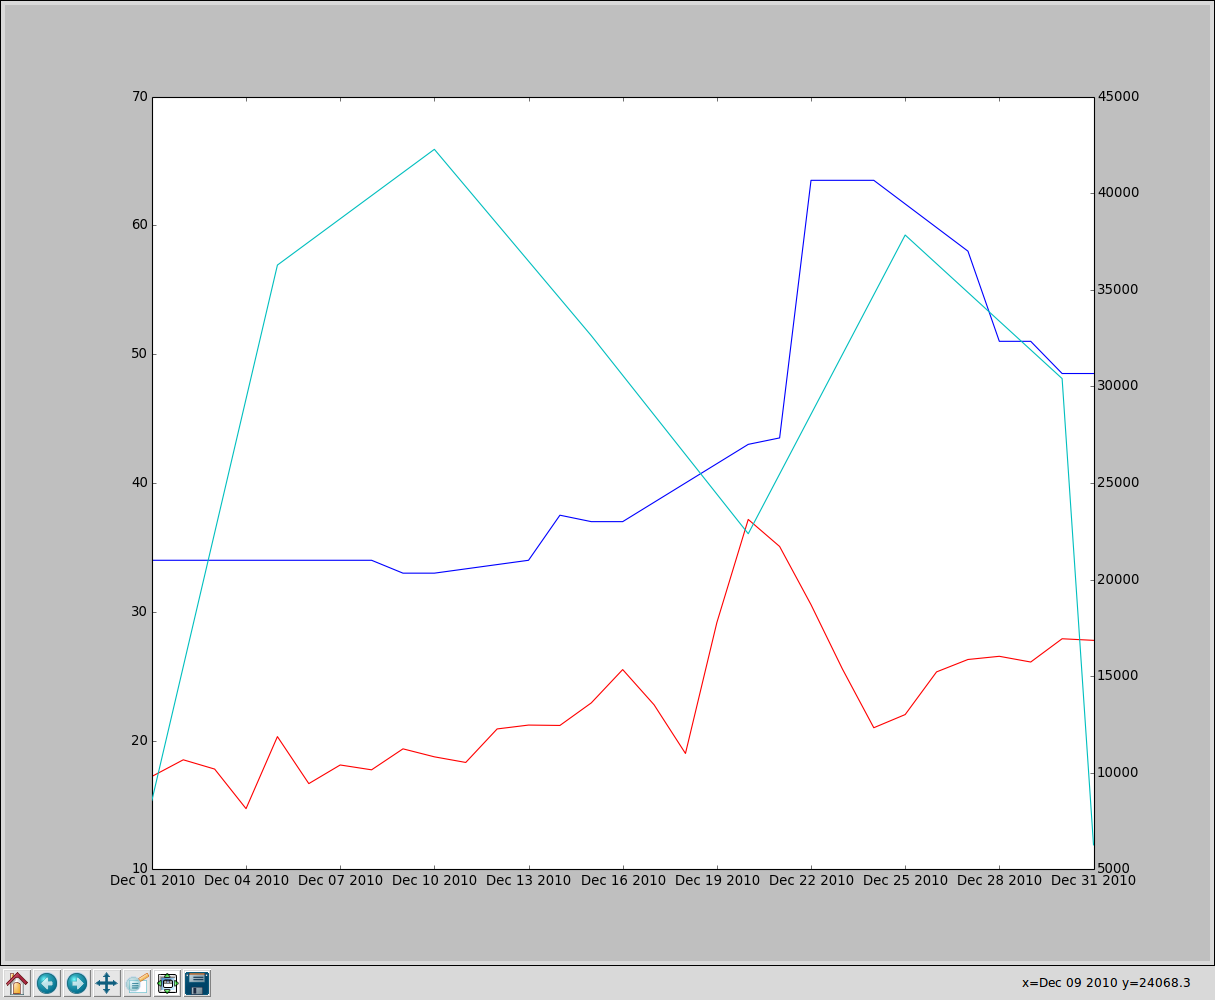
\includegraphics[scale=0.3]{2010_dec_maha}
\caption{Maharashtra, Dec 2010. (Blue - Retail price, Red - Wholesale Price, Cyan - Arrival)}
\label{fig:MaharashtraDec2010}
\end{center}
\end{figure}

\begin{figure}[h]
\begin{center}    
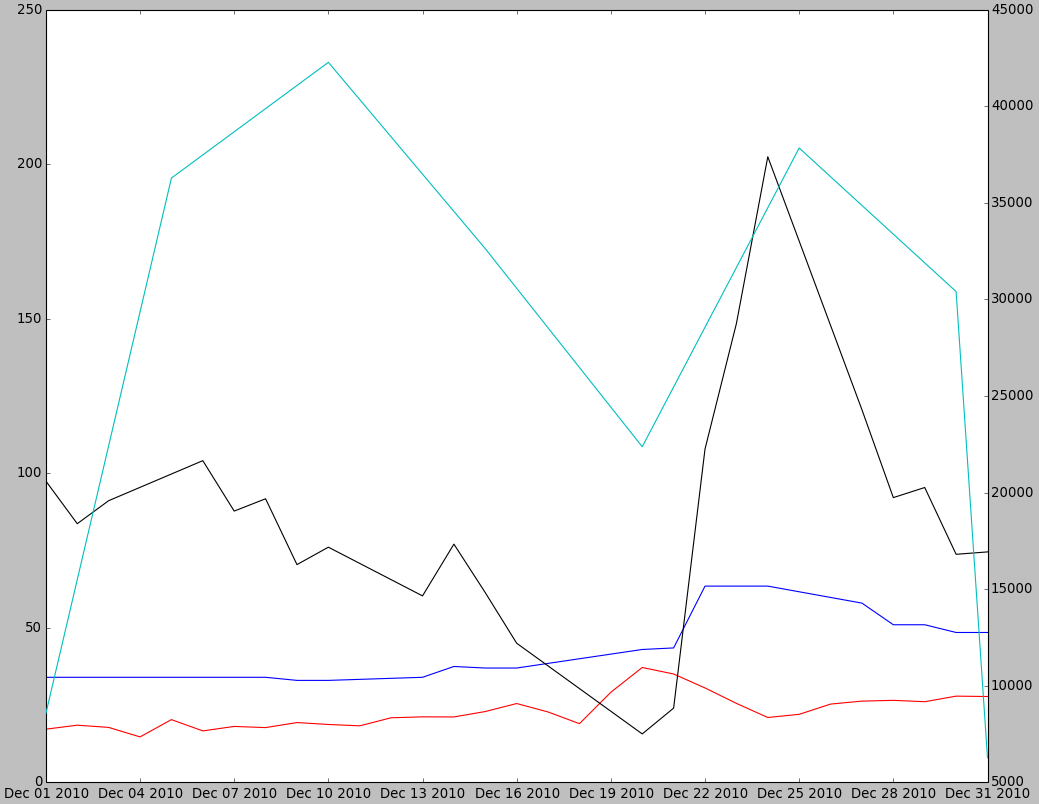
\includegraphics[scale=0.3]{2010_dec_maha_relative}
\caption{Maharashtra Dec 2010. (Blue - Retail price, Red - Wholesale Price, Cyan - Arrival, Black - Relative difference \%)}
\label{fig:MaharashtraDec2010Relativedifference}
\end{center}
\end{figure}

\begin{figure}[h]
\begin{center}    
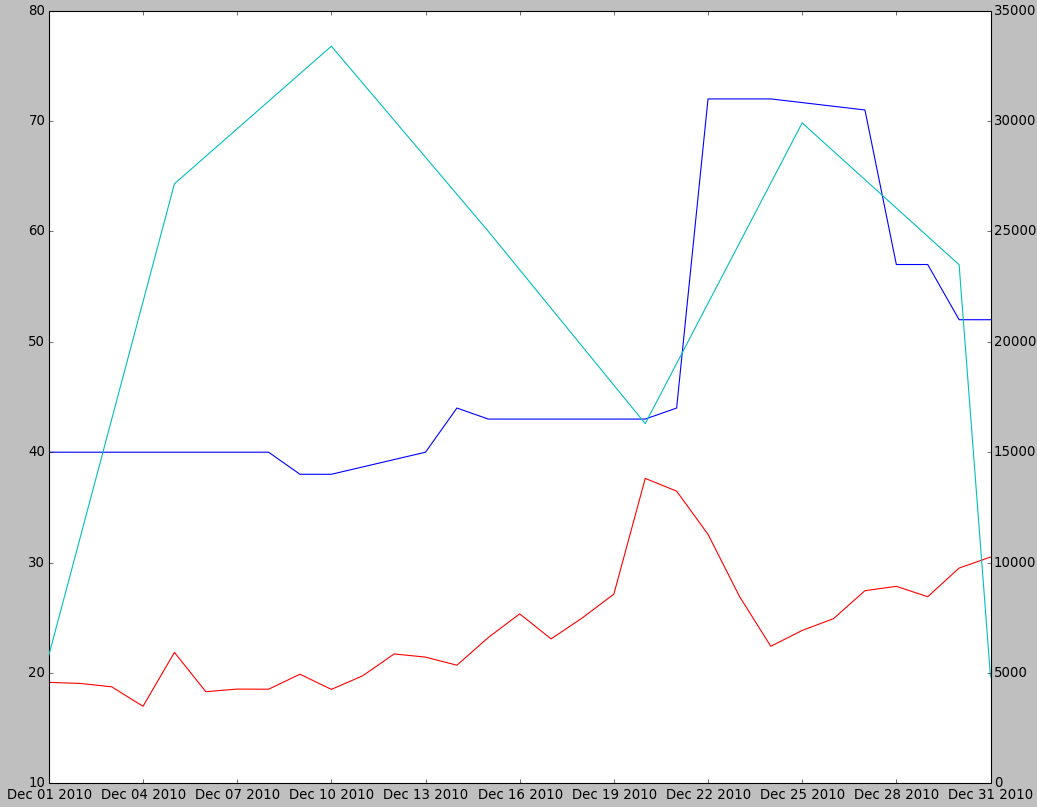
\includegraphics[scale=0.3]{2010_dec_mumbai}
\caption{Mumbai , Dec 2010. (Blue - Retail price, Red - Wholesale Price, Cyan - Arrival)}
\label{fig:MumbaiDec2010}
\end{center}
\end{figure}

\begin{figure}[h]
\begin{center}    
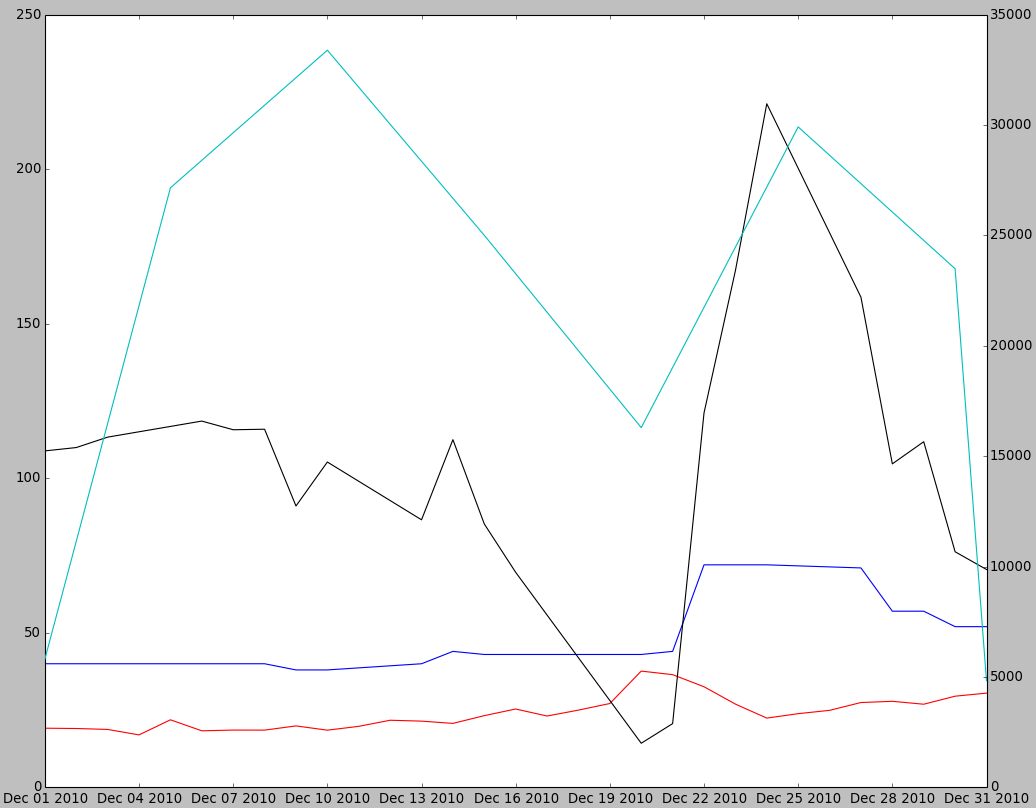
\includegraphics[scale=0.3]{2010_dec_mumbai_relative}
\caption{Mumbai, Dec 2010. (Blue - Retail price, Red - Wholesale Price, Cyan - Arrival Black - Relative difference \%)}
\label{fig:MumbaiDec2010Relativedifference}
\end{center}
\end{figure}

As we can see from the Figures \ref{fig:MaharashtraDec2010}, \ref{fig:MaharashtraDec2010Relativedifference}, \ref{fig:MumbaiDec2010} and \ref{fig:MumbaiDec2010Relativedifference}, the difference between retail and wholesale went as much high as 200\% in both overall Maharashtra as well as in the Mumbai. Also, as per report \cite{Theg88:online}, this trend was also continued in the next month, i.e. January 2011, which can be seen in the following graph. (See figures \ref{fig:MumbaiJan2011} and \ref{fig:MumbaiJan2011Relativediff})

\begin{figure}[h]
\begin{center}    
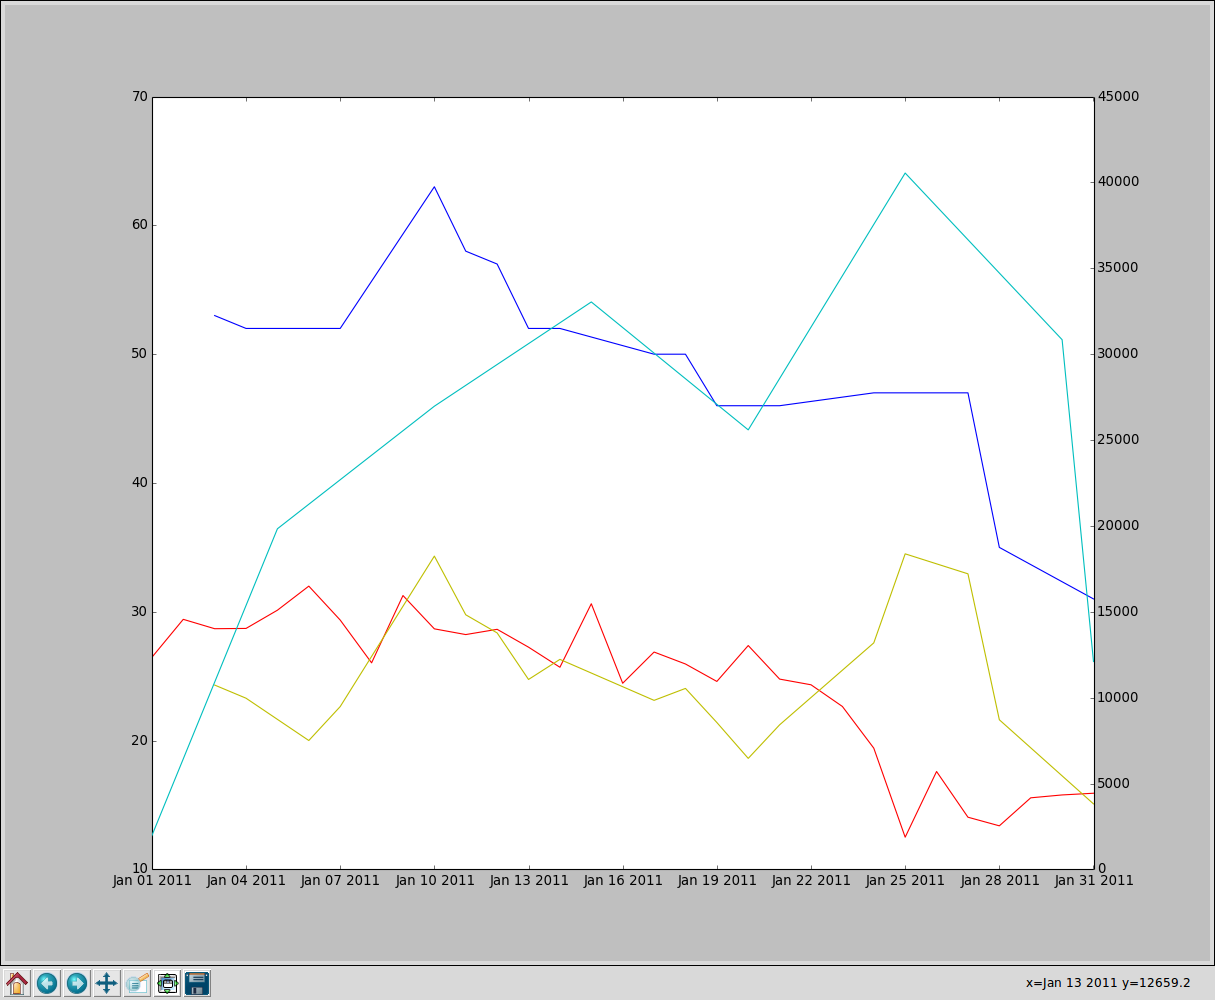
\includegraphics[scale=0.3]{2011_jan_mumbai}
\caption{Mumbai , Jan 2011. (Blue - Retail price, Red - Wholesale Price, Cyan - Arrival)}
\label{fig:MumbaiJan2011}
\end{center}
\end{figure}

\begin{figure}[h]
\begin{center}    
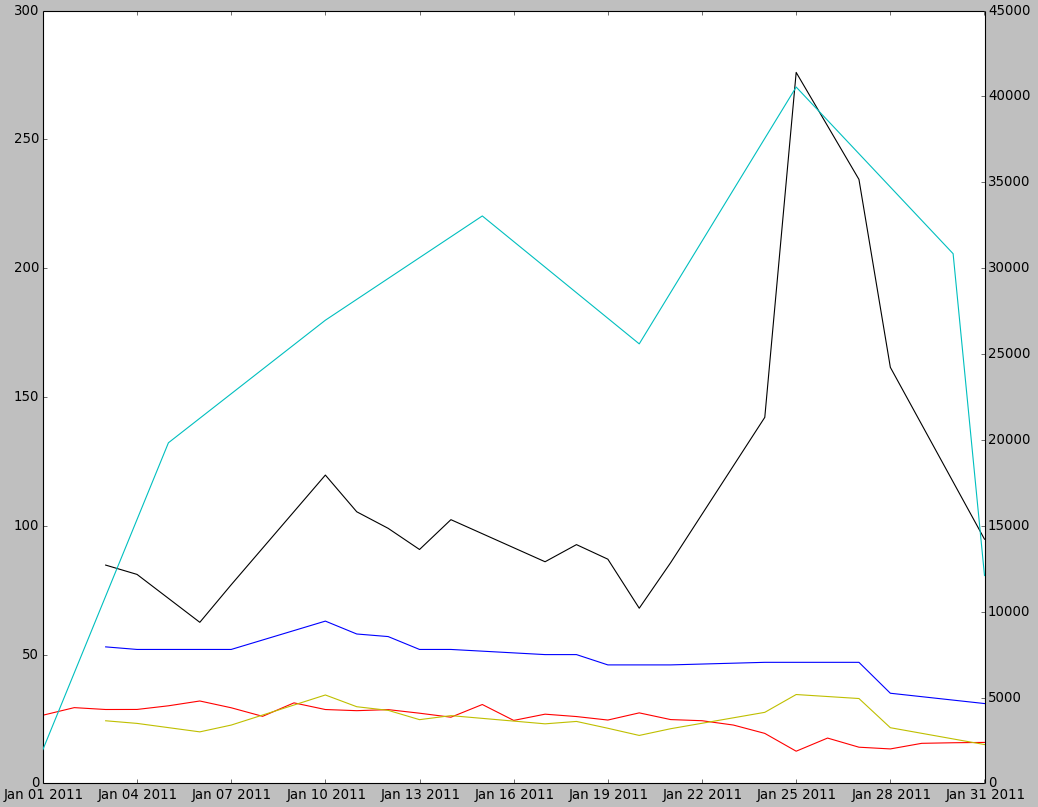
\includegraphics[scale=0.3]{2011_jan_mumbai_relative_diff}
\caption{Mumbai, Jan 2011. (Blue - Retail price, Red - Wholesale Price, Cyan - Arrival Black - Relative difference \%)}
\label{fig:MumbaiJan2011Relativediff}
\end{center}
\end{figure}

Next hoarding news was reported in the last week July 2013. As per the Business Standard Report \cite{Flyin19:online},

“Onion prices in Nashik, Pune and Ahmednagar have increased to Rs 2,400 a quintal as on July 21, compared to Rs 1,500-1,800 a quintal during the corresponding period of last year. Arrival of onions in Nashik, which contributes 35-40 per cent to the state production, has been 83,000 quintals compared with 82,000 quintals last year”

Also, In the month of August, September and October of 2013, the price rise of the Onion in various parts of countries like Banglore (\cite{Onion55:online}), New Delhi (\cite{Hoard62:online},\cite{Onion85:online},\cite{Noon17:online}) and Gandhinagar ([\cite{Govt81:online}) was in the news. Reports of Banglore and New Delhi has just reported the hike in the retail price. DNA report on Gandhinagar says,

“Retail onion prices in the city have increased from around Rs40/kg, a month ago, to Rs70/kg on Saturday. In the wholesale market, onion prices have increased around Rs35 per kg till last week to Rs45 per kg on Saturday. The wholesale price is Rs.40 to 45 per kg. Ideally, in the retail market the price should not be more than Rs.60 per kg”

Let's look at the data we have. As from the figures \ref{fig:MumbaiJuly2012} and \ref{fig:MumbaiJuly2013}, the wholesale rates around the mandis present around the Mumbai in the month of July, 2012 was about Rs. 5/Kg, but during the same time period in the 2013, the wholesale prices went from Rs. 15/Kg to Rs. 25/Kg. Although, there was decrement in the arrival by 7\% as compared to July 2012, but the rise in the wholesale price is very much high.

\begin{figure}[h]
\begin{center}    
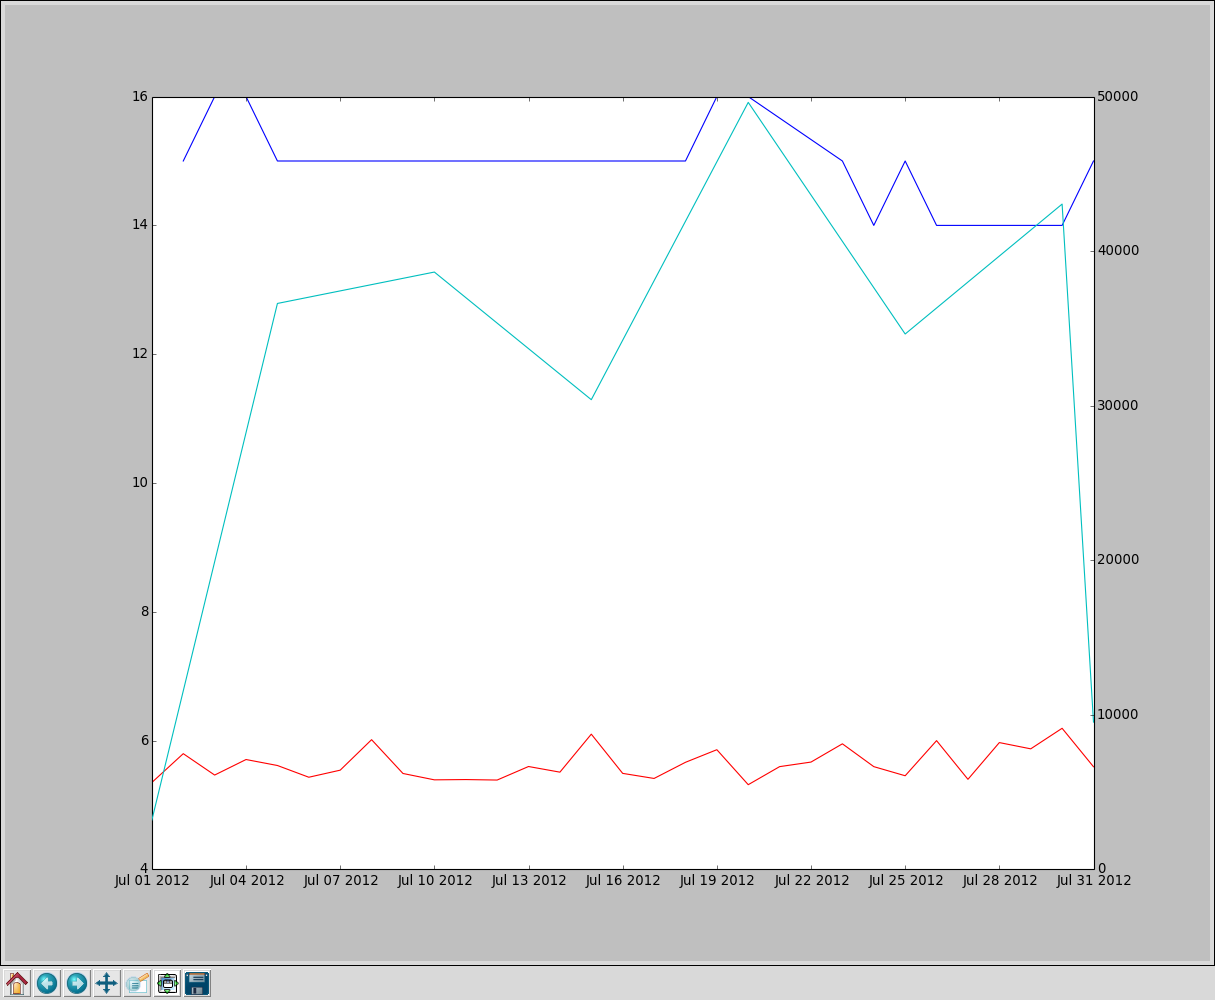
\includegraphics[scale=0.3]{2012_jul_mumbai}
\caption{Mumbai , July 2012. (Blue - Retail price, Red - Wholesale Price, Cyan - Arrival)}
\label{fig:MumbaiJuly2012}
\end{center}
\end{figure}

\begin{figure}[h]
\begin{center}    
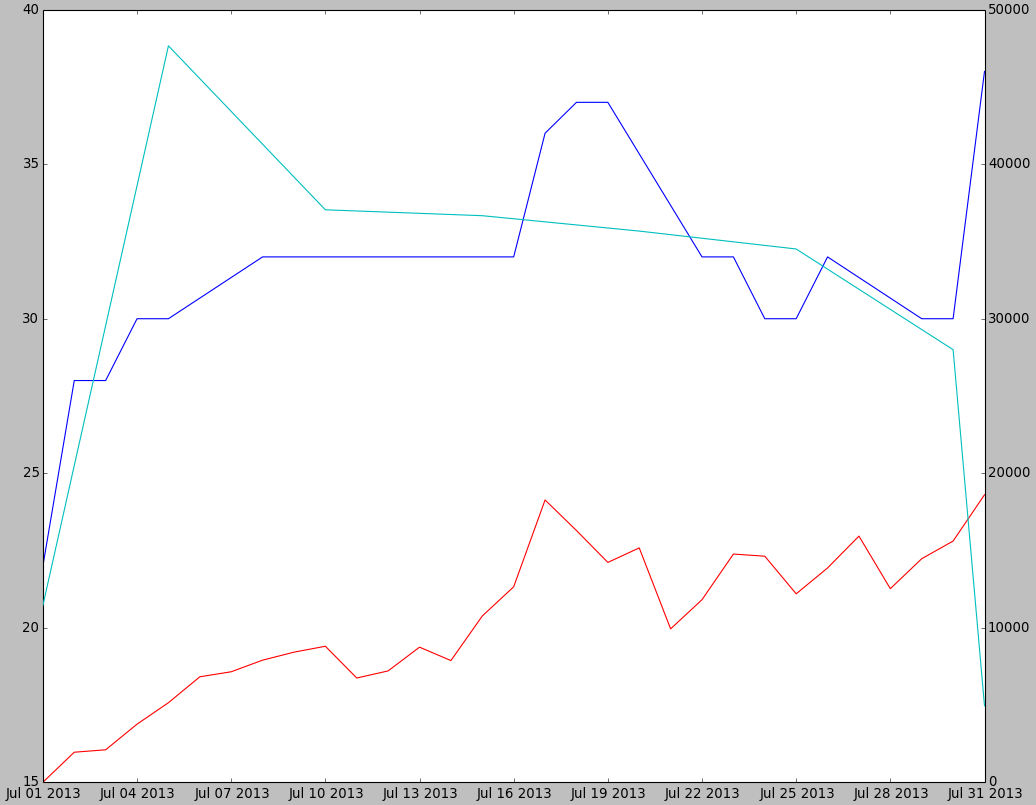
\includegraphics[scale=0.3]{2013_july_mumbai}
\caption{Mumbai , July 2013. (Blue - Retail price, Red - Wholesale Price, Cyan - Arrival)}
\label{fig:MumbaiJuly2013}
\end{center}
\end{figure}


Figures \ref{fig:AhmedabadAug2013} and \ref{fig:RajkotAug2013}, states the scenario of Gujarat. There also the wholesale as well as the retail prices became suddenly almost double in the month of August 2013.

\begin{figure}[h]
\begin{center}    
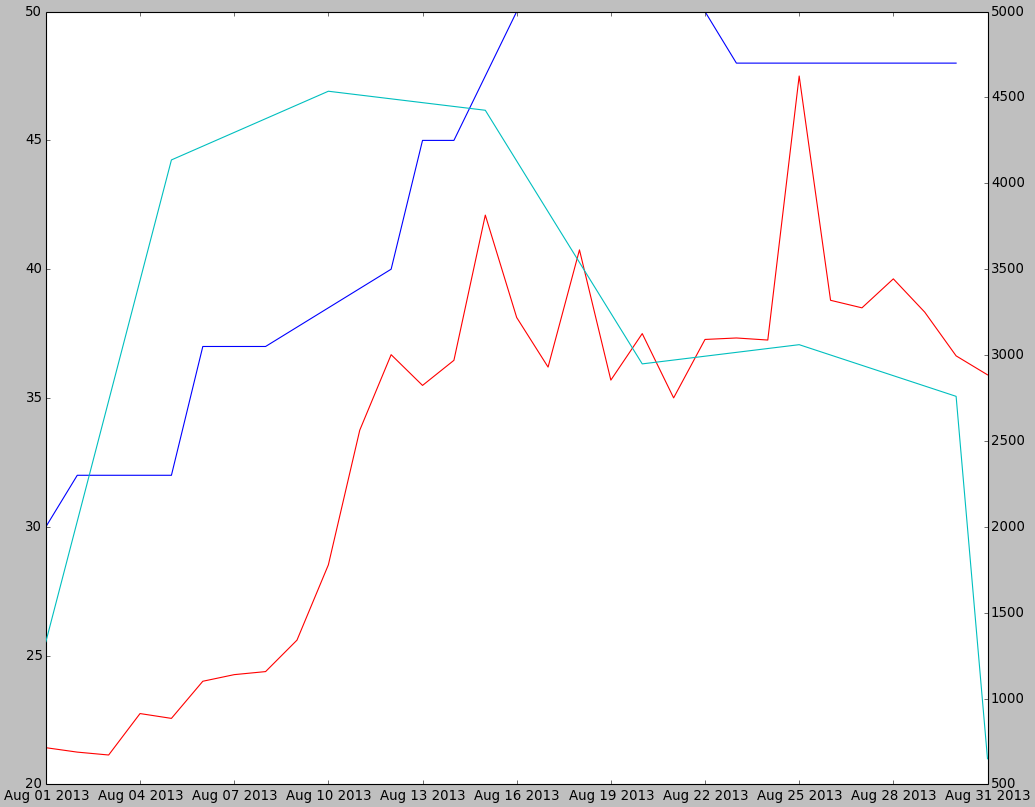
\includegraphics[scale=0.3]{2013_aug_ahmdb}
\caption{Ahmedabad , Aug 2013. (Blue - Retail price, Red - Wholesale Price, Cyan - Arrival)}
\label{fig:AhmedabadAug2013}
\end{center}
\end{figure}

\begin{figure}[h]
\begin{center}    
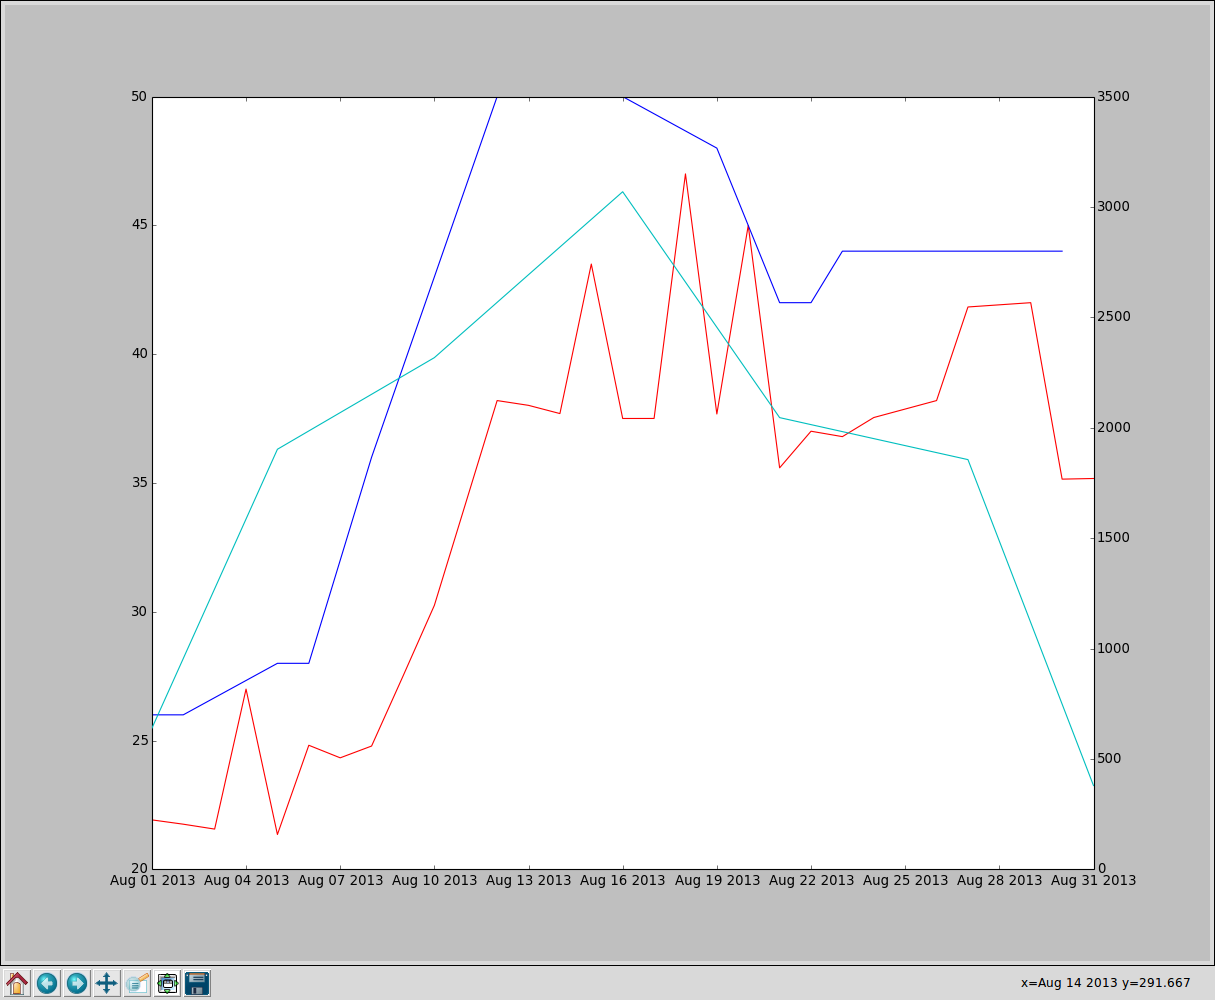
\includegraphics[scale=0.3]{2013_aug_rajkot}
\caption{Rajkot , Aug 2013. (Blue - Retail price, Red - Wholesale Price, Cyan - Arrival)}
\label{fig:RajkotAug2013}
\end{center}
\end{figure}

Also, in year 2014, price hike of Onions was in the news. There were reports from Mumbai \cite{Onion68:online}, Kerala \cite{Keral99:online} and Hydrabad \cite{Rains78:online} which stated the hike in the prices of the onion. Let's look at the graph of the Mumbai for the year of 2014. As we can see from the graph (Figure \ref{fig:Mumbai2014}) that for the period of July to October the wholesale price were decreasing, but still that was not reflected in the retail price and instead of decreasing, the retail price kept on increasing.


\begin{figure}[h]
\begin{center}    
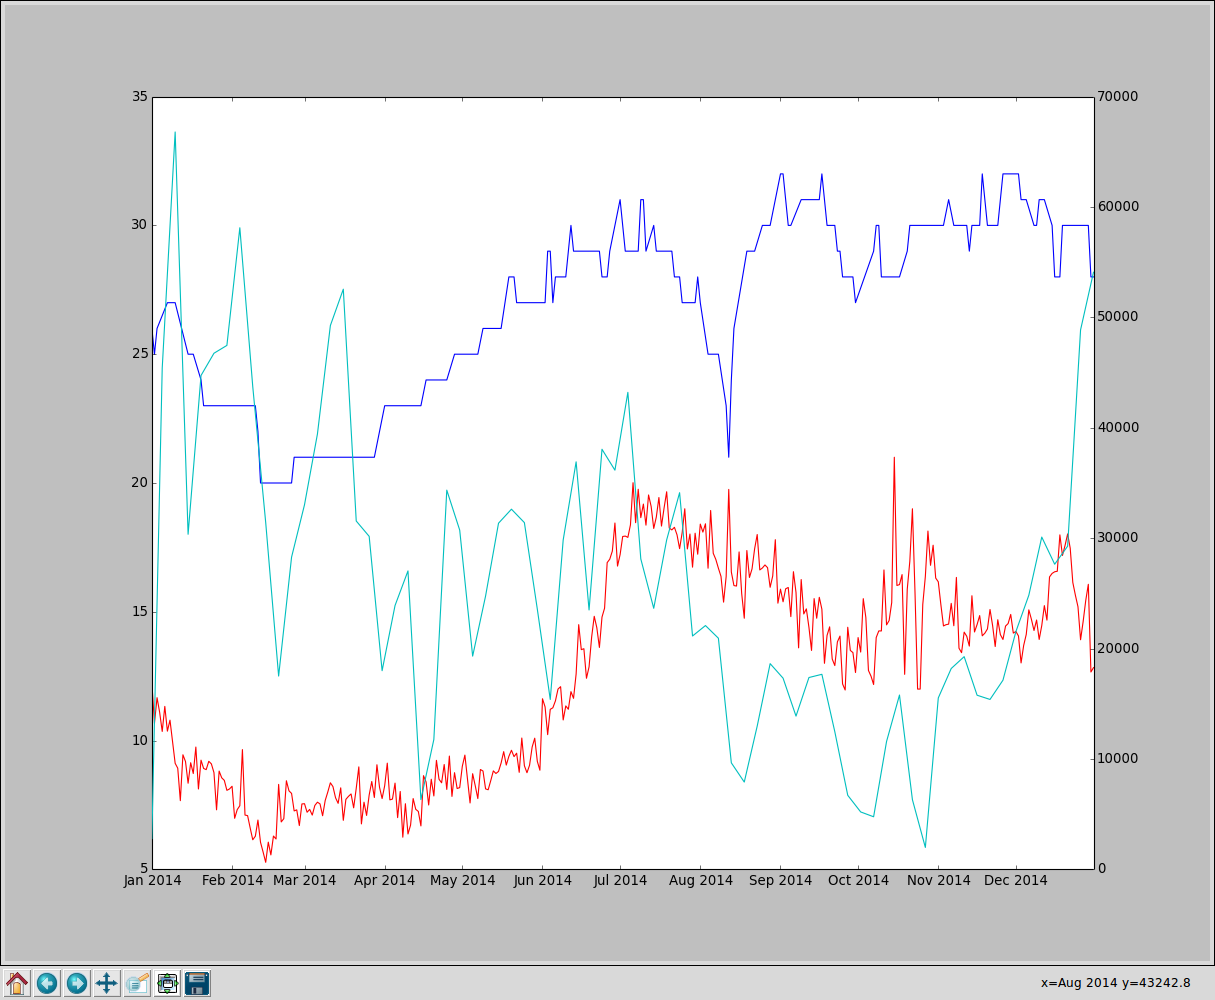
\includegraphics[scale=0.3]{2014_mumbai}
\caption{Mumbai , 2014. (Blue - Retail price, Red - Wholesale Price, Cyan - Arrival)}
\label{fig:Mumbai2014}
\end{center}
\end{figure}

\section{Characteristics of anomaly}

Hoarding of commodities in excess, results in anomaly. We segregated news articles on hoarding of onion and tried to spot some characteristics of data for anomalies.

So, major characteristics of hoarding spotted in newspapers are following:

\begin{enumerate}
\item Huge difference in wholesale and retail prices
\item Sudden rise in wholesale or retail price
\item Rise in wholesale prices when arrival is enough/high
\end{enumerate}

We can also generalize anomaly cases as shown in table \ref{table:1} and \ref{table:2}. The estimated arrival, wholesale and retail price data is labeled up, down and constant based on if it exceeds actual data value. Red flags are raised based on the following tables if the condition falls under the category marked with {\color{red}A}’s.


\begin{table}
\centering
\begin{tabular}{ | c | c | c | c |}  
  \hline
  \textbf{W$\backslash$A} & \textbf{$\uparrow$} & \textbf{$\leftrightarrow$}  & \textbf{$\downarrow$} \\ \hline
  \textbf{$\uparrow$} & - & {\color{red}A} & {\color{red}A} \\ \hline
  \textbf{$\leftrightarrow$} & - & - & {\color{red}A} \\ \hline
  \textbf{$\downarrow$} & - & - & - \\ \hline
\end{tabular}
\caption{Anomaly Scenarios - 1}
\label{table:1}
\end{table}

\begin{table}
\centering
\begin{tabular}{ | c | c | c | c |}  
  \hline
  \textbf{W$\backslash$A} & \textbf{$\uparrow$} & \textbf{$\leftrightarrow$}  & \textbf{$\downarrow$} \\ \hline
  \textbf{$\uparrow$} & {\color{red}A} & {\color{red}A} & - \\ \hline
  \textbf{$\leftrightarrow$} & {\color{red}A} & - & - \\ \hline
  \textbf{$\downarrow$} & - & - & - \\ \hline
\end{tabular}
\caption{Anomaly Scenarios - 2}
\label{table:2}
\end{table}

\section{Hypothesis}

So from the above analysis of all news reports, we conclude four hypothesis.

Wholesale price is inversely proportional to arrival in the market and we assume it is the only factor on which wholesale price is dependent. We also noticed in our literature review that most of the farmers don’t hoard in India. So, from this relation, we have the following hypothesis:

\textbf{\textit{H1. If there is increase in arrival pattern, there should be decrease in the wholesale price and if there is decrease in arrival pattern, there should be increase in the wholesale price considering a lag factor of 15 days.}}

Retailers purchase onions from the wholesale markets, mandis, etc. So, rate at retail level should be directly proportional to wholesale price in that region. We assume here that demand remains constant and there is no supply shock created because of excessive export of onion So from here we get the following hypothesis.

\textbf{\textit{H2. If there is increase in the wholesale price of onion, then there will be corresponding increase in the retail price and vice-versa assuming demand remains constant and there is no supply shock created because of excessive export of onion.}}

Similarly, we can state that if there is no change in the arrival for some period, then wholesale may remain same and if wholesale price remains same for some period than retail price may remain same. So from that we get following two hypothesis:

\textbf{\textit{H3. The deviation between arrival - wholesale and wholesale- retail should not vary much compared to values for same time in past years.}}

Also, one should make a note of that, even in H1 and H2, when wholesale price or retail is increasing, then it should be in considerable amount. It should not be like, there is marginal increase in wholesale price and retail price is boosting up or there is little decrement in arrival and wholesale price goes up by unacceptable level.

Also, we assume that mandis in the same region will behave in similar manner, because production and effect of other factors will be same in one region. So, based on that we have following hypothesis:

\textbf{\textit{H4. Mandis in the same region should follow the same relationship between arrival and wholesale price, as that of, taken whole region combinely.}}

Our attempt would be to create a library which takes all these series as an input and try to detect possibilities of above stated anomalies or highlight all the important unusual behavior of parameters seen in the input series.




\chapter{Proposed Design and Framework}


\section{System Design}

\begin{figure}[here]
\begin{center}    
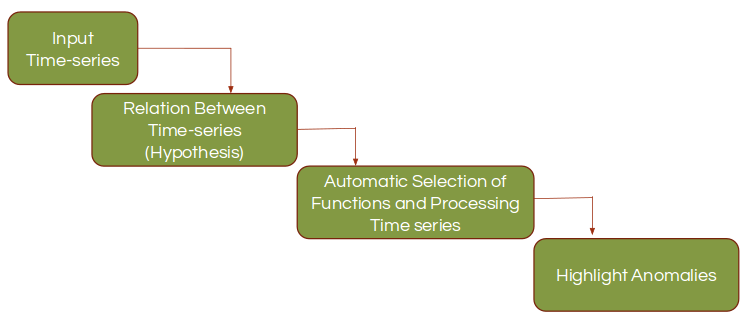
\includegraphics[scale=0.5]{System}
\caption{System Design}
\label{fig:SystemDesign}
\end{center}
\end{figure}


So figure \ref{fig:SystemDesign} explains the overall design of the system and its modules. We have made some assumption regarding system as follows:

\begin{enumerate}

\item Given time series should be of the same time period.
\item Each time series should be present in different file.

\end{enumerate}

\subsection {Input Time-series}

Here, give option to user to input number of time series and accordingly, provide option to select time series in CSV format. Currently, we have thought of keeping restriction that CSV file should contain only one time series. Also, ask user whether he wants to smooth time series or not. Smoothing of time series will be done using Exponential Moving Average technique. $\alpha$  factor for same will be considered as \[ 2 / (1+ period) \].  Where period is considered as up to how much of previous values should have effect on today's value. By default, we have kept it as 14. If user has technical knowledge then option to select period can be provided.

\subsection {Relation Between Time-series (Hypothesis)}

Normal behavior of the time series should be stated somehow, so that we can detect anomaly in the data. So, to get this input from user, we will be providing \textit{n*n} matrix with some default value, where '\textit{n}' corresponds to the number of time series user gave as an input. Now by filling each cell in the matrix, user can specify the relation between any 2 time series as follows:


\begin{itemize}

\item \textbf{1:} Positive Correlation
\item \textbf{-1:} negative Correlation
\item \textbf{0:} Random Relation
\item \textbf{2:} User is not aware but is interested in finding relation, if exist any
\item \textbf{Default:} User is not aware of any relation and also any doesn’t exist according to user

\end{itemize}

If correlation exists, then we may also take input from user maximum lag factor to consider. If not provided any, then by default it will be taken as -15 to +15. We may also ask user, whether to consider only positive lag, negative lag or both types of lag.

\subsection {Automatic Selection of Functions and Processing Time series}

Now, after taking proper input, it is time to execute appropriate function for each of the provided input types.

\subsection {Highlight Anomalies}

After execution, display what tests were performed and what were their results. Detailed values will be provided if asked specifically. Different Graphs/Charts possible with the output can be generated on user demand. Provide an option to user whether he would like to see the results with some different threshold value other than the taken by library. Provide all the functionalities present in the system and ask user, if he wants to run some specific tests on the input time series.

\section{Test Criterion for Hypothesis}

In the last chapter, we stated some hypothesis. Now, here we state what tests can be performed to detect anomalies for each of the hypothesis.

\subsection{Hypothesis 1}

\begin{itemize}

\item Starting with granularity of year-wise, find out cross-correlation, considering various lag factor up to 15,  between arrival and wholesale and check that overall it is positive or negative.

\item Go on decrease the granularity. Next will be season-wise. For a particular season, how arrival and wholesale price are behaving. Point out where, this correlation becomes positive.

\item Similar thing can be done for month-wise as well as fortnight data.

\item Note that, correlation mentioned here is just one of the method. There can be various other methods to define the behavior of 2 time-series.

\item \textbf{Slope Based Detection:} Calculate the slope of both time-series daywise and compare. \textit{Assumption:} Data is smoothed. Since day-wise is taken, if data is not smoothed then it may generate many “spikes”. So if data is not smoothed, then before applying this technique, either apply smoothing or take weekly average. If granularity of data is daywise, then smoothing can help. If data is reported once-twice weekly, then taking average weekly and then calculating slope day-wise may help.

\item \textbf{Linear Regression Based Method:} We can train model using linear regression. Then find out the difference between actual and predicted value for each of the data point and plot a histogram. From these points we can try to find out points which are going very much out of the way using method like MAD test.

\end{itemize}

\subsection{Hypothesis 2}

\begin{itemize}

\item Starting with granularity of year-wise, find out cross-correlation, considering various lag factor up to 15,  between arrival and wholesale and check that overall it is positive or negative.

\item Go on decrease the granularity. Next will be season-wise. For a particular season, how arrival and wholesale price are behaving. Point out where, this correlation becomes positive.

\item Similar thing can be done for month-wise as well as fortnight data.

\item Note that, correlation mentioned here is just one of the method. There can be various other methods to define the behavior of 2 time-series.

\item \textbf{Slope Based Detection:} Calculate the slope of both time-series daywise and compare. \textit{Assumption:} Data is smoothed. Since day-wise is taken, if data is not smoothed then it may generate many “spikes”. So if data is not smoothed, then before applying this technique, either apply smoothing or take weekly average. If granularity of data is daywise, then smoothing can help. If data is reported once-twice weekly, then taking average weekly and then calculating slope day-wise may help.

\item \textbf{Linear Regression Based Method:} We can train model using linear regression. Then find out the difference between actual and predicted value for each of the data point and plot a histogram. From these points we can try to find out points which are going very much out of the way using method like MAD test.

\item Spike Detection methods

\end{itemize}

\subsection{Hypothesis 3}

\begin{itemize}

\item One can use prediction based model like ARIMA \cite{arima} to test this hypothesis. If method mentioned in \cite{arima} is used then there is no need to align time-series into phase, as method mentioned in it take care of it. One can train the model considering some period for 8 years and can be tested on remaining 2 years. Difference in actual and predicted value is seen and one above some threshold value is reported. Also, while generating model, different window size can be considered. If some other technique is used, then one may need to align time series into common phase. That can be done using cross-correlation method, considering lag factor of around 15 days. Lag with the highest correlation value is considered.

\item One can also apply graph based anomaly detection technique as mentioned in \cite{nasa} to find out malicious behavior.

\end{itemize}

\subsection{Hypothesis 4}


Here, we need to combine data of multiple places into one, to find out the combined behavior and then compare it with each of the mandi. One of the technique, to combine multiple series is,

\begin{itemize}

\item For Arrivals: take sum from all Mandis
\item For Wholesale-price: Take average
\item Apart from center, if one wants to combine statewise, then for retail price also, one can take average for retail price

\end{itemize}

Other technique, to combine multiple time series is, subspace based transformation, as mentioned in \cite{phdthesisdc}. Then, to compare behavior of each particular mandi time-series with the aggregated one, techniques mentioned to test hypothesis 1 or 2 can be used.

\textbf{Note (Applicable to Onion Case):} Results returned by H1 and H2, consists of all the time periods where arrival-wholesale price and wholesale price-retail price pairs go out of line. There may be case where, for each time of that year it may be going out of line and might not be anomaly. So, to remove such false positives, we can take intersection of results of H1 and results of H3. Similar thing can be done with H2 also, by taking  intersection of results of H2 and results of H3.




\chapter{Results and Analysis}

We executed our library functions on the onion data. This data consists of 
Wholesale Price, Retail Price and Arrival since 1st January 2006 to 6th July 
2015. In this chapter, we will show results produced by our system and will 
analyse these results along with each method.

\section{Results}

We have performed 4 types of analysis and result for each of this method is as 
follows. Note that these are primary results. Data for 2 centres are considered 
- Mumbai and Delhi.\\
\\
Here are some results related with Mumbai Center. Table \ref{AnomaliesReported} shows the result of anomalies reported by our system, with details about anomalies reported by each method. So here First 5 columns corresponds to each method. Column 6 is union of results of first 3 methods and column 7 is union of results of method 4 and 5, as described in table. Column 8 is intersection of results of column 6 and column 7, which is final result of our system.\\
\\
Table \ref{ArticlesMatched} shows the result of number of articles matched with the dates reported by our system as anomaly for each method. So here First 5 columns corresponds to each method. Column 6 is union of results of first 3 methods and column 7 is union of result of method 4 and 5, as described in table. Column 8 is intersection of results of column 6 and column 7, which is final result of our system.\\
\\
Note that total number of articles present for center Mumbai is \textbf{99} and all these articles are present after 2010. Apart from Graph Based Anomaly and Multivariate- vector autoregressive method, all methods are producing results from 2006 onwards as input data is from that time. The following pie chart(see figure \ref{fig:pieReasons}) shows the analysis of article showing what news articles states as the reason for the price hikes of onion.\\
\\
\begin{figure}[H]
\centering
\begin{tikzpicture}
   \pie[ text = legend ]{32/Traders Nexus, 18/Not Stated, 10/Unseasonal Rainfall, 12/Low Production, 18/Low Supply, 10/Other  }
\end{tikzpicture}
\caption{Reasons stated by news articles for onion price hike}
\label{fig:pieReasons}
\end{figure}

% First here about +5, -5

While finding the news article match for every anomaly, we check for all the news articles 5 days before and 5 days after the reported date. In case we find any news article in this tenure, we consider it as a match for that date. For one date of anomaly, multiple articles may be present but for this analysis we have considered only the nearest article for that anomaly date. Following bar charts represents distribution of how far is the news article from the date of anomaly.

\begin{figure}[H]
\centering
\begin{tikzpicture}
\begin{axis}[
	x tick label style={
		/pgf/number format/1000 sep=},
	ylabel=Number of Articles,
	enlargelimits=0.05,
	legend style={at={(0.5,-0.1)},
	anchor=north,legend columns=-1},
	ybar interval=0.7,
]
\addplot 
	coordinates {(-5,3)(-4,4)(-3,5)(-2,4)(-1,6)(0,16)(1,10)(2,5)(3,4)(4,3)(5,4)(6,0)};

\end{axis}
\end{tikzpicture}
\caption{Article Distribution for Retail Price VS Average Retail Price}
\label{fig:articleDistRvsR}
\end{figure}

\begin{figure}[H]
\centering
\begin{tikzpicture}
\begin{axis}[
	x tick label style={
		/pgf/number format/1000 sep=},
	ylabel=Number of Articles,
	enlargelimits=0.05,
	legend style={at={(0.5,-0.1)},
	anchor=north,legend columns=-1},
	ybar interval=0.7,
]
\addplot 
	coordinates {(-5,8)(-4,9)(-3,11)(-2,13)(-1,16)(0,34)(1,21)(2,14)(3,11)(4,8)(5,8)(6,0)};

% \legend{Men,Women}
\end{axis}
\end{tikzpicture}
\caption{Article Distribution for Retail Price VS Arrival Of Onion}
\label{fig:articleDistRvsA}
\end{figure}


\begin{figure}[H]
\centering
\begin{tikzpicture}
\begin{axis}[
	x tick label style={
		/pgf/number format/1000 sep=},
	ylabel=Number of Articles,
	enlargelimits=0.05,
	legend style={at={(0.5,-0.1)},
	anchor=north,legend columns=-1},
	ybar interval=0.7,
]
\addplot 
	coordinates {(-5,4)(-4,5)(-3,6)(-2,5)(-1,3)(0,9)(1,5)(2,3)(3,5)(4,3)(5,4)(6,0)};

% \legend{Men,Women}
\end{axis}
\end{tikzpicture}
\caption{Article Distribution for Wholesale Price VS Retail Price}
\label{fig:articleDistRvsW}
\end{figure}


\begin{figure}[H]
\centering
\begin{tikzpicture}
\begin{axis}[
	x tick label style={
		/pgf/number format/1000 sep=},
	ylabel=Number of Articles,
	enlargelimits=0.05,
	legend style={at={(0.5,-0.1)},
	anchor=north,legend columns=-1},
	ybar interval=0.7,
]
\addplot 
	coordinates {(-5,8)(-4,10)(-3,11)(-2,13)(-1,17)(0,37)(1,25)(2,16)(3,13)(4,9)(5,9)(6,0)};

% \legend{Men,Women}
\end{axis}
\end{tikzpicture}
\caption{Article Distribution for Wholesale Price VS Arrival Of Onion}
\label{fig:articleDistWvsA}
\end{figure}


Now, we present detailed analysis for each of the different type of time-series. First type of such analysis is in table \ref{RetailVsAverage}. This table shows distribution of news articles present (that matched with system results) year-wise for each method when retail price time series is compared with average retail price time series. Second type of such analysis is in table \ref{RetailVsArrival}. This table shows distribution of news articles present year-wise for each method when retail price time series is compared with arrival data of onion time series. Third type of such analysis is in table \ref{RetailVsWholesale}. This table shows distribution of news articles present year-wise for each method when retail price time series is compared with wholesale price time series. Fourth type of such analysis is in table \ref{WholesaleVsArrival}. This table shows distribution of news articles present year-wise for each method when wholesale price time series is compared with arrival data of onion time series.\\
\\
Distribution of anomalies present year-wise, for each method is also shown in table. Result for various analysis is described in tables  \ref{RetailVsAverageDist}, \ref{RetailVsArrivalDist}, \ref{RetailVsWholesaleDist} and \ref{WholesaleVsArrivalDist}.\\
\\
Such results for different cities can also be calculated.

  
	\begin{table}[]
	\centering
	
	\resizebox{\textwidth}{!}
	{\begin{tabular}{|l|l|l|l|l|l|l|l|l|}
	\hline
	Methods              & Slope Based (1) & Correlation (2) & Linear Regression (3) & Graph Based (4) & Multivariate (5) & 1 U 2 U 3 (6) & 4 U 5 (7) & 6 $\cap$ 7  \\
	\hline
	Retail Vs Average    & 742 & 255 & 353 & 300 & 177 & 1206 & 362 & 125 \\
	\hline
	Retail Vs Arrival    & 420 & 795 & 353 & 500 & 167 & 1381 & 573 & 323 \\
	\hline
	Retail Vs Wholesale  & 658 & 420 & 310 & 300 & 167 & 1243 & 367 & 160 \\
	\hline
	Wholesale Vs Arrival & 448 & 705 & 282 & 500 & 186 & 1315 & 586 & 332 \\
	\hline
	\end{tabular}}
	\caption{Anomalies Reported}
	\label{AnomaliesReported}
	\end{table}
      
	\begin{table}[]
	\centering
	
	\resizebox{\textwidth}{!}
	{\begin{tabular}{|l|l|l|l|l|l|l|l|l|}
	\hline
	Methods              & Slope Based (1) & Correlation (2) & Linear Regression (3) & Graph Based (4) & Multivariate (5) & 1 U 2 U 3 (6) & 4 U 5 (7) & 6 $\cap$ 7   \\
	\hline
	Retail Vs Average    & 67 & 47 & 50  & 122 & 122 & 142 & 162 & 64  \\
	\hline
	Retail Vs Arrival    & 42 & 74 & 167 & 121 & 119 & 220 & 159 & 153 \\
	\hline
	Retail Vs Wholesale  & 30 & 55 & 40  & 117 & 119 & 107 & 150 & 52  \\
	\hline
	Wholesale Vs Arrival & 64 & 64 & 174 & 122 & 139 & 219 & 174 & 168 \\
	\hline
	\end{tabular}}
	\caption{Number of news articles matched with system}
	\label{ArticlesMatched}
	\end{table}
	
      

	\begin{table}[]
	\centering
	\resizebox{\textwidth}{!}
	{\begin{tabular}{|l|l|l|l|l|l|l|l|l|l|}
	\hline
	Distribution of All Articles & Articles Present & Slope Based (1) & Correlation (2) & Linear Regression (3) & Graph Based (4) & Multivariate (5) & 1 U 2 U 3 (6) & 4 U 5 (7) & 6 $\cap$ 7 \\
	\hline
	2010 & 6  & 0  & 0  & 8  & 10 & 0   & 8  & 10  & 3  \\
	\hline
	2011 & 3  & 0  & 0  & 0  & 12 & 0   & 0  & 12  & 0  \\
	\hline
	2012 & 2  & 1  & 0  & 0  & 0  & 0   & 1  & 0   & 0  \\
	\hline
	2013 & 54 & 42 & 14 & 18 & 86 & 119 & 61 & 125 & 61 \\
	\hline
	2014 & 23 & 24 & 0  & 24 & 14 & 3   & 39 & 15  & 0  \\
	\hline
	2015 & 11 & 0  & 33 & 0  & 0  & 0   & 33 & 0   & 0  \\
	\hline
	\end{tabular}}	
	\caption{Retail Price VS Average Retail Price}
	\label{RetailVsAverage}
	\end{table}
	
	
	
	\begin{table}[]
	\centering
	\resizebox{\textwidth}{!}
	{\begin{tabular}{|l|l|l|l|l|l|l|l|l|l|}
	\hline
	Distribution of All Articles & Articles Present & Slope Based (1) & Correlation (2) & Linear Regression (3) & Graph Based (4) & Multivariate (5) & 1 U 2 U 3 (6) & 4 U 5 (7) & 6 $\cap$ 7  \\
	\hline
	2010 & 6  & 17 & 0  & 17  & 17 & 0   & 17  & 17  & 17  \\
	\hline
	2011 & 3  & 1  & 0  & 12  & 12 & 0   & 12  & 12  & 12  \\
	\hline
	2012 & 2  & 0  & 0  & 0   & 0  & 0   & 0   & 0   & 0   \\
	\hline
	2013 & 54 & 10 & 39 & 126 & 92 & 119 & 137 & 130 & 124 \\
	\hline
	2014 & 23 & 14 & 35 & 12  & 0  & 0   & 54  & 0   & 0   \\
	\hline
	2015 & 11 & 0  & 0  & 0   & 0  & 0   & 0   & 0   & 0  \\
	\hline
	\end{tabular}}	
	\caption{Retail Price VS Arrival data of onion}
	\label{RetailVsArrival}
	\end{table}

	
	
	
	\begin{table}[]
	\centering
	\resizebox{\textwidth}{!}
	{\begin{tabular}{|l|l|l|l|l|l|l|l|l|l|}
	\hline
	Distribution of All Articles & Articles Present & Slope Based (1) & Correlation (2) & Linear Regression (3) & Graph Based (4) & Multivariate (5) & 1 U 2 U 3 (6) & 4 U 5 (7) & 6 $\cap$ 7 \\
	\hline
	2010 & 6  & 6  & 0  & 2  & 11 & 0   & 6  & 11  & 6  \\
	\hline
	2011 & 3  & 1  & 0  & 0  & 4  & 0   & 1  & 4   & 1  \\
	\hline
	2012 & 2  & 2  & 7  & 0  & 0  & 0   & 7  & 0   & 0  \\
	\hline
	2013 & 54 & 7  & 21 & 18 & 91 & 119 & 45 & 124 & 44 \\
	\hline
	2014 & 23 & 14 & 27 & 20 & 11 & 0   & 48 & 11  & 1  \\
	\hline
	2015 & 11 & 0  & 0  & 0  & 0  & 0   & 0  & 0   & 0 \\
	\hline
	\end{tabular}}	
	\caption{Retail Price VS Wholesale Price}
	\label{RetailVsWholesale}
	\end{table}

	
	
	\begin{table}[]
	\centering
	\resizebox{\textwidth}{!}
	{\begin{tabular}{|l|l|l|l|l|l|l|l|l|l|}
	\hline
	Distribution of All Articles & Articles Present & Slope Based (1) & Correlation (2) & Linear Regression (3) & Graph Based (4) & Multivariate (5) & 1 U 2 U 3 (6) & 4 U 5 (7) & 6 $\cap$ 7  \\
	\hline
	2010 & 6  & 17 & 0  & 17  & 17 & 0   & 17  & 17  & 17  \\
	\hline
	2011 & 3  & 1  & 0  & 12  & 12 & 0   & 12  & 12  & 12  \\
	\hline
	2012 & 2  & 0  & 0  & 0   & 0  & 0   & 0   & 0   & 0   \\
	\hline
	2013 & 54 & 25 & 15 & 125 & 93 & 123 & 129 & 129 & 123 \\
	\hline
	2014 & 23 & 21 & 49 & 20  & 0  & 16  & 61  & 16  & 16  \\
	\hline
	2015 & 11 & 0  & 0  & 0   & 0  & 0   & 0   & 0   & 0   \\
	\hline
	\end{tabular}}	
	\caption{ Wholesale Price VS Arrival data of onion}
	\label{WholesaleVsArrival}
	\end{table}
	
	
	
	
	\begin{table}[]
	\centering
	\resizebox{\textwidth}{!}
	{\begin{tabular}{|l|l|l|l|l|l|l|l|l|}
	\hline
	Distribution of All Articles & Slope Based (1) & Correlation (2) & Linear Regression (3) & Graph Based (4) & Multivariate (5) & 1 U 2 U 3 (6) & 4 U 5 (7) & 6 $\cap$ 7 \\
	\hline
	2006 & 133 & 30 & 65  & 0   & 0   & 204 & 0   & 0  \\
	\hline
	2007 & 14  & 15 & 30  & 0   & 0   & 53  & 0   & 0  \\
	\hline
	2008 & 42  & 15 & 0   & 0   & 0   & 47  & 0   & 0  \\
	\hline
	2009 & 82  & 15 & 0   & 0   & 0   & 96  & 0   & 0  \\
	\hline
	2010 & 72  & 45 & 28  & 37  & 0   & 142 & 37  & 13 \\
	\hline
	2011 & 56  & 60 & 115 & 57  & 0   & 182 & 57  & 9  \\
	\hline
	2012 & 84  & 0  & 33  & 13  & 0   & 100 & 13  & 5  \\
	\hline
	2013 & 77  & 15 & 56  & 134 & 161 & 125 & 189 & 90 \\
	\hline
	2014 & 140 & 0  & 26  & 40  & 16  & 155 & 47  & 8  \\
	\hline
	2015 & 42  & 60 & 0   & 19  & 0   & 102 & 19  & 0  \\
	\hline
	\end{tabular}}
	\caption{Distribution of Anomalies reported by system for Retail Price VS Average Retail Price}
	\label{RetailVsAverageDist}
	\end{table}
	  
	  
	  
	
	\begin{table}[]
	\centering
	\resizebox{\textwidth}{!}
	{\begin{tabular}{|l|l|l|l|l|l|l|l|l|}
	\hline
	Distribution of All Articles & Slope Based (1) & Correlation (2) & Linear Regression (3) & Graph Based (4) & Multivariate (5) & 1 U 2 U 3 (6) & 4 U 5 (7) & 6 $\cap$ 7  \\
	\hline
	2006 & 35 & 185 & 0   & 0   & 0   & 199 & 0   & 0   \\
	\hline
	2007 & 63 & 85  & 0   & 0   & 0   & 148 & 0   & 0   \\
	\hline
	2008 & 28 & 105 & 0   & 0   & 0   & 126 & 0   & 0   \\
	\hline
	2009 & 28 & 45  & 0   & 0   & 0   & 73  & 0   & 0   \\
	\hline
	2010 & 48 & 60  & 46  & 143 & 0   & 107 & 143 & 56  \\
	\hline
	2011 & 36 & 60  & 40  & 165 & 0   & 128 & 165 & 65  \\
	\hline
	2012 & 77 & 45  & 0   & 81  & 0   & 118 & 81  & 25  \\
	\hline
	2013 & 59 & 90  & 168 & 111 & 161 & 263 & 178 & 172 \\
	\hline
	2014 & 46 & 105 & 99  & 0   & 6   & 204 & 6   & 5   \\
	\hline
	2015 & 0  & 15  & 0   & 0   & 0   & 15  & 0   & 0   \\
	\hline
	\end{tabular}}
	\caption{Distribution of Anomalies reported by system for Retail Price VS Arrival data of onion }
	\label{RetailVsArrivalDist}
	\end{table}
	
	
	\begin{table}[]
	\centering
	\resizebox{\textwidth}{!}
	{\begin{tabular}{|l|l|l|l|l|l|l|l|l|}
	\hline
	Distribution of All Articles & Slope Based (1) & Correlation (2) & Linear Regression (3) & Graph Based (4) & Multivariate (5) & 1 U 2 U 3 (6) & 4 U 5 (7) & 6 $\cap$ 7  \\
	\hline
	2006 & 126 & 0  & 0  & 0   & 0   & 126 & 0   & 0  \\
	\hline
	2007 & 77  & 30 & 0  & 0   & 0   & 107 & 0   & 0  \\
	\hline
	2008 & 70  & 15 & 0  & 0   & 0   & 85  & 0   & 0  \\
	\hline
	2009 & 63  & 75 & 0  & 0   & 0   & 126 & 0   & 0  \\
	\hline
	2010 & 62  & 30 & 2  & 53  & 0   & 92  & 53  & 8  \\
	\hline
	2011 & 50  & 45 & 67 & 75  & 0   & 155 & 75  & 34 \\
	\hline
	2012 & 72  & 82 & 64 & 7   & 0   & 160 & 7   & 0  \\
	\hline
	2013 & 50  & 38 & 44 & 105 & 161 & 124 & 166 & 81 \\
	\hline
	2014 & 60  & 75 & 99 & 60  & 6   & 182 & 66  & 37 \\
	\hline
	2015 & 28  & 30 & 34 & 0   & 0   & 86  & 0   & 0  \\
	\hline
	\end{tabular}}
	\caption{Distribution of Anomalies reported by system for Retail Price VS Wholesale Price }
	\label{RetailVsWholesaleDist}
	\end{table}
	
	
	\begin{table}[]
	\centering
	\resizebox{\textwidth}{!}
	{\begin{tabular}{|l|l|l|l|l|l|l|l|l|}
	\hline
	Distribution of All Articles & Slope Based (1) & Correlation (2) & Linear Regression (3) & Graph Based (4) & Multivariate (5) & 1 U 2 U 3 (6) & 4 U 5 (7) & 6 $\cap$ 7  \\
	\hline
	2006 & 0  & 65  & 0   & 0   & 0   & 65  & 0   & 0   \\
	\hline
	2007 & 42 & 100 & 0   & 0   & 0   & 142 & 0   & 0   \\
	\hline
	2008 & 21 & 120 & 0   & 0   & 0   & 141 & 0   & 0   \\
	\hline
	2009 & 56 & 60  & 0   & 0   & 0   & 109 & 0   & 0   \\
	\hline
	2010 & 83 & 75  & 51  & 142 & 0   & 162 & 142 & 62  \\
	\hline
	2011 & 64 & 60  & 34  & 165 & 0   & 157 & 165 & 67  \\
	\hline
	2012 & 42 & 45  & 0   & 81  & 0   & 87  & 81  & 12  \\
	\hline
	2013 & 80 & 45  & 157 & 112 & 152 & 246 & 164 & 157 \\
	\hline
	2014 & 46 & 105 & 40  & 0   & 34  & 162 & 34  & 34  \\
	\hline
	2015 & 14 & 30  & 0   & 0   & 0   & 44  & 0   & 0   \\
	\hline
	\end{tabular}}
	\caption{Distribution of Anomalies reported by system for Wholesale Price VS Arrival data of onion }
	\label{WholesaleVsArrivalDist}
	\end{table}
	

\section{Analysis of Each Method}

In this section, we try to analyse strengths, weaknesses and limitations of every method. So, we will describe each method one by one. Note that we have articles from 2010 onwards, so we will be focussing on anomalies reported after 2010 and compare them with the news articles we have. \\
\\
\textbf{Note that all the graphs and results described in following sections are for centre Mumbai. Mumbai is in Maharashtra state, which is the largest producer of onion in India. Also in graphs, Yellow highlighted region corresponds to anomalies reported by system, red region corresponds to dates for which our system reported anomaly and news article was present for that and blue region corresponds to date for which news article was present but that date was not reported as anomaly by our system.}

\subsection{Slope Based Anomaly Detection}
	
		The main functionality of this method is to find change in one variable with respect to other. Given two time-series, here we try to find, between two points in time series, how much dependent variable changed corresponding to independent variable. If this change is huge, then it is reported as anomaly.\\
		\\
		We have four types of analysis which are as following:
		\begin{enumerate}
			\item \textbf{Retail Price vs Average of Retail Price}: Here, we first take average of retail price at all centres and than compare change in retail price with respect to change in average of retail price for different time window.			
			\item \textbf{Retail Price vs Arrival of Onion}: Here, we try to find change in retail price with respect to change in arrival of onion for different windows. 
			\item \textbf{Retail Price vs Wholesale Price}: Here, retail price is dependent on wholesale price and we try to find change in retail price with respect to change wholesale price for different windows.
			\item \textbf{Wholesale Price vs Arrival of Onion}: Here, we try to find change in wholesale price with respect to change in arrival of onion for different window size.
		\end{enumerate}
		
		So, in each of the case, we try to find change with respect to another, and if this change is huge, crossing threshold than it is reported as anomaly. Note that in analysis 1 and 3 stated above, both the time series are directly proportional to each other and in the analysis 2 and 4 both the time series are inversely proportional to each other. So, limitations faced by this method for analysis 1 and 3 will be similar and for analysis 2 and 4 will be similar. While describing this method, each analysis will be referenced by its corresponding number.\\
		\\
		First we will start with analysis 1 and 3. Following are the few observations:
		
			
		\begin{itemize}
		
			\item In case of analysis 1, dates are reported as anomalies if retail price at centre is increasing more as compared to average retail price and in case of analysis 3, it is reported if retail price at centre is increasing more as compared to wholesale price. \\
			Following tenures are some cases reported by this method:
			\begin{itemize}
				\item \textit{Analysis 1}: June 2010, August 2010, May 2011, June 2011, May Jun Nov 2012, Apr May 2013 (Prices went too high as compared to average) (See Figure \ref{fig:12111})
				\item \textit{Analysis 3}: Apr July Oct Dec 2010, Jan 2011, May June 2014 (See Figure \ref{fig:12131})
			\end{itemize}
			\begin{figure}[H]
		    	\centering
  		    	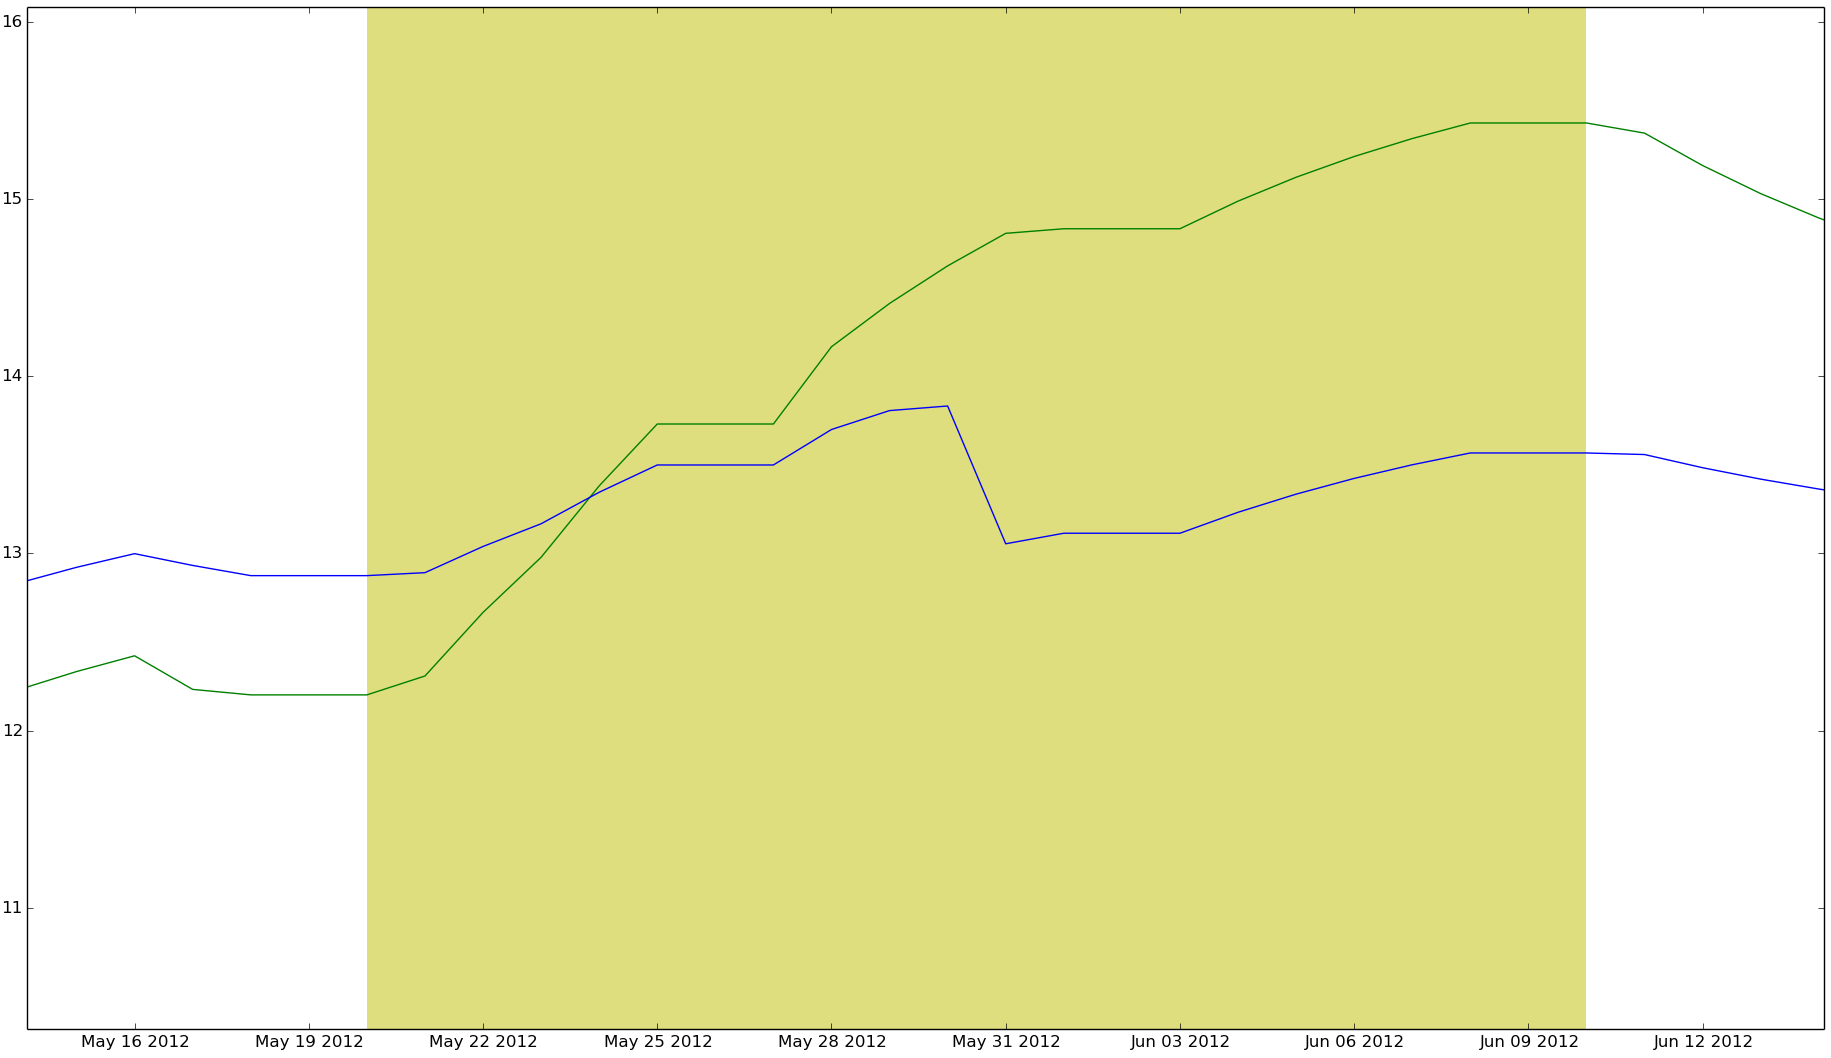
\includegraphics[width=0.8\textwidth]{graphs/12111.png}
		    	\caption{Slope Based Anomaly Detection (Green line - Centre Retail Price, Blue Line - Average Retail Price)}
		    	\label{fig:12111}
			\end{figure}
			
			\begin{figure}[H]
		    	\centering
  		    	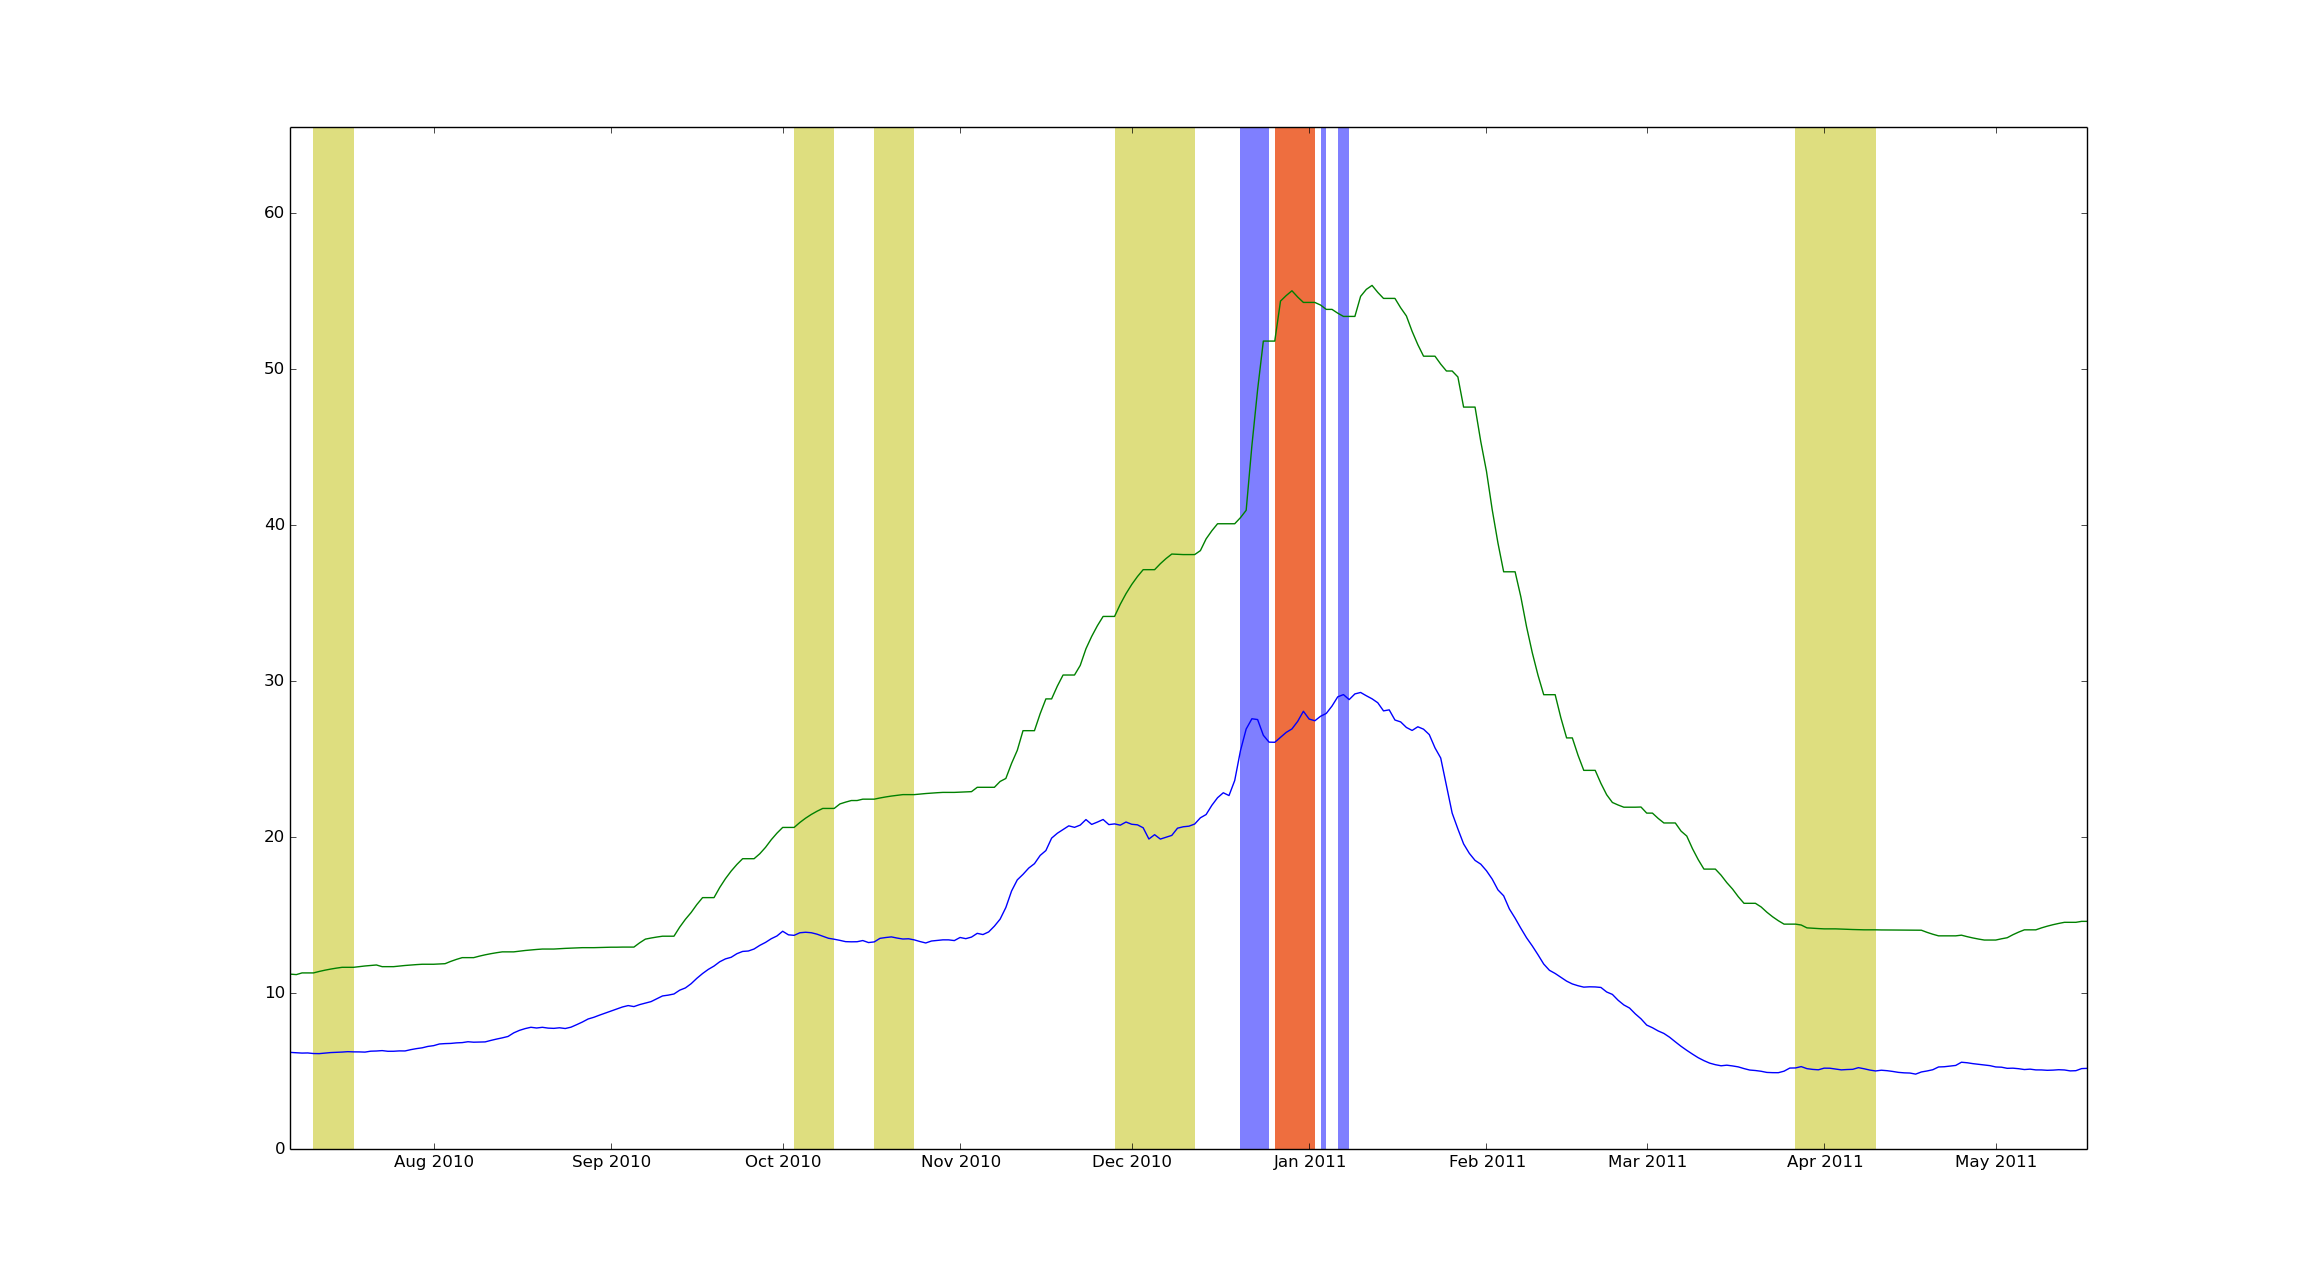
\includegraphics[width=0.8\textwidth]{graphs/12131.png}
		    	\caption{Slope Based Anomaly Detection (Green line - Retail Price, Blue Line - Wholesale Price)}
		    	\label{fig:12131}
			\end{figure}
			
			
			
			So, even though we do not have articles for these anomalies, but method is behaving as it should be. 			
			
			\item One of the limitation for this method is that there are some cases where drop in retail price for one center is quite huge as compared to drop in average retail price (in case of \textit{analysis 1}) or wholesale price (in case of \textit{analysis 3}). This is good thing for customers at that centre and should not be treated as anomaly. But in this case, slope value goes high and that's why our method reports that tenure as anomaly.\\
			Following tenures are some cases reported by this method:
			\begin{itemize}
				\item \textit{Analysis 1}: January 2010, June Aug 2012, Jan 2013, Feb Oct 2014, Feb 2015  (See Figure \ref{fig:12112})
				\item \textit{Analysis 3}: Feb May 2010  (See Figure \ref{fig:12132})
			\end{itemize}
			
			\begin{figure}[H]
		    	\centering
  		    	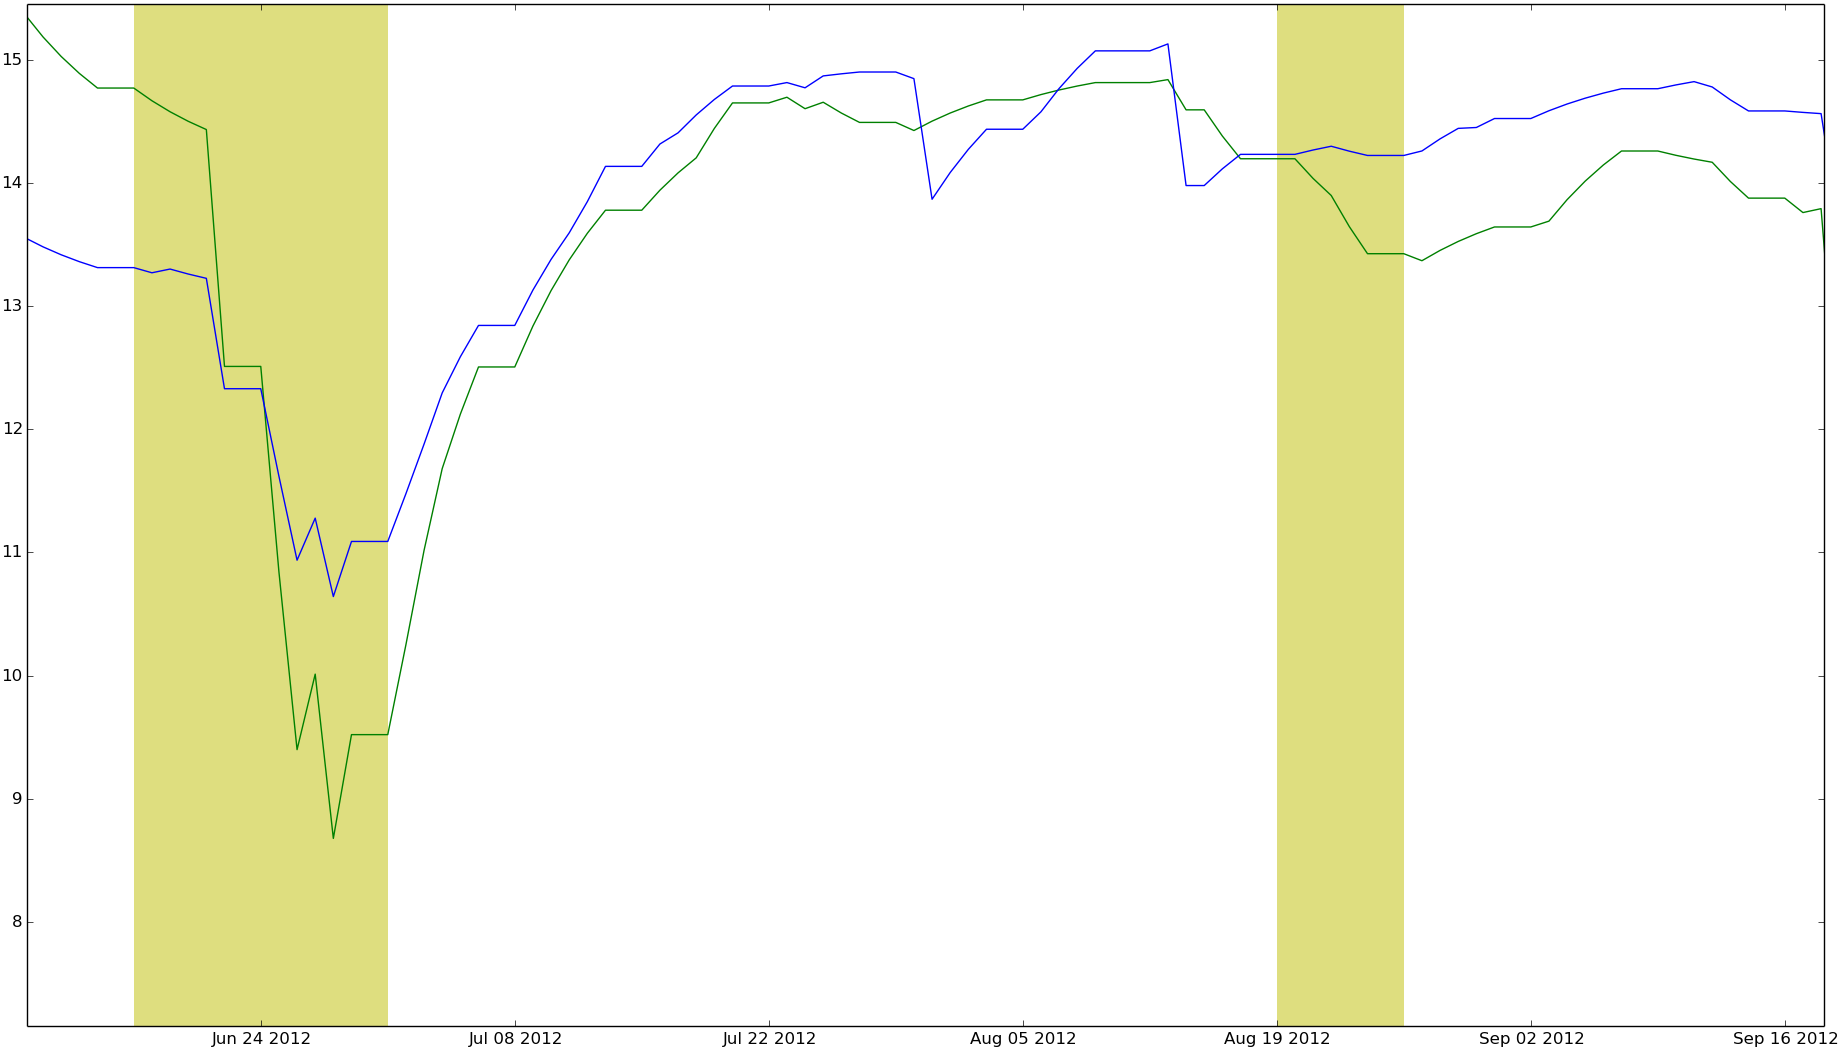
\includegraphics[width=0.8\textwidth]{graphs/12112.png}
		    	\caption{Slope Based Anomaly Detection (Green line - Centre Retail Price, Blue Line - Average Retail Price)}
		    	\label{fig:12112}
			\end{figure}
			
			\begin{figure}[H]
		    	\centering
  		    	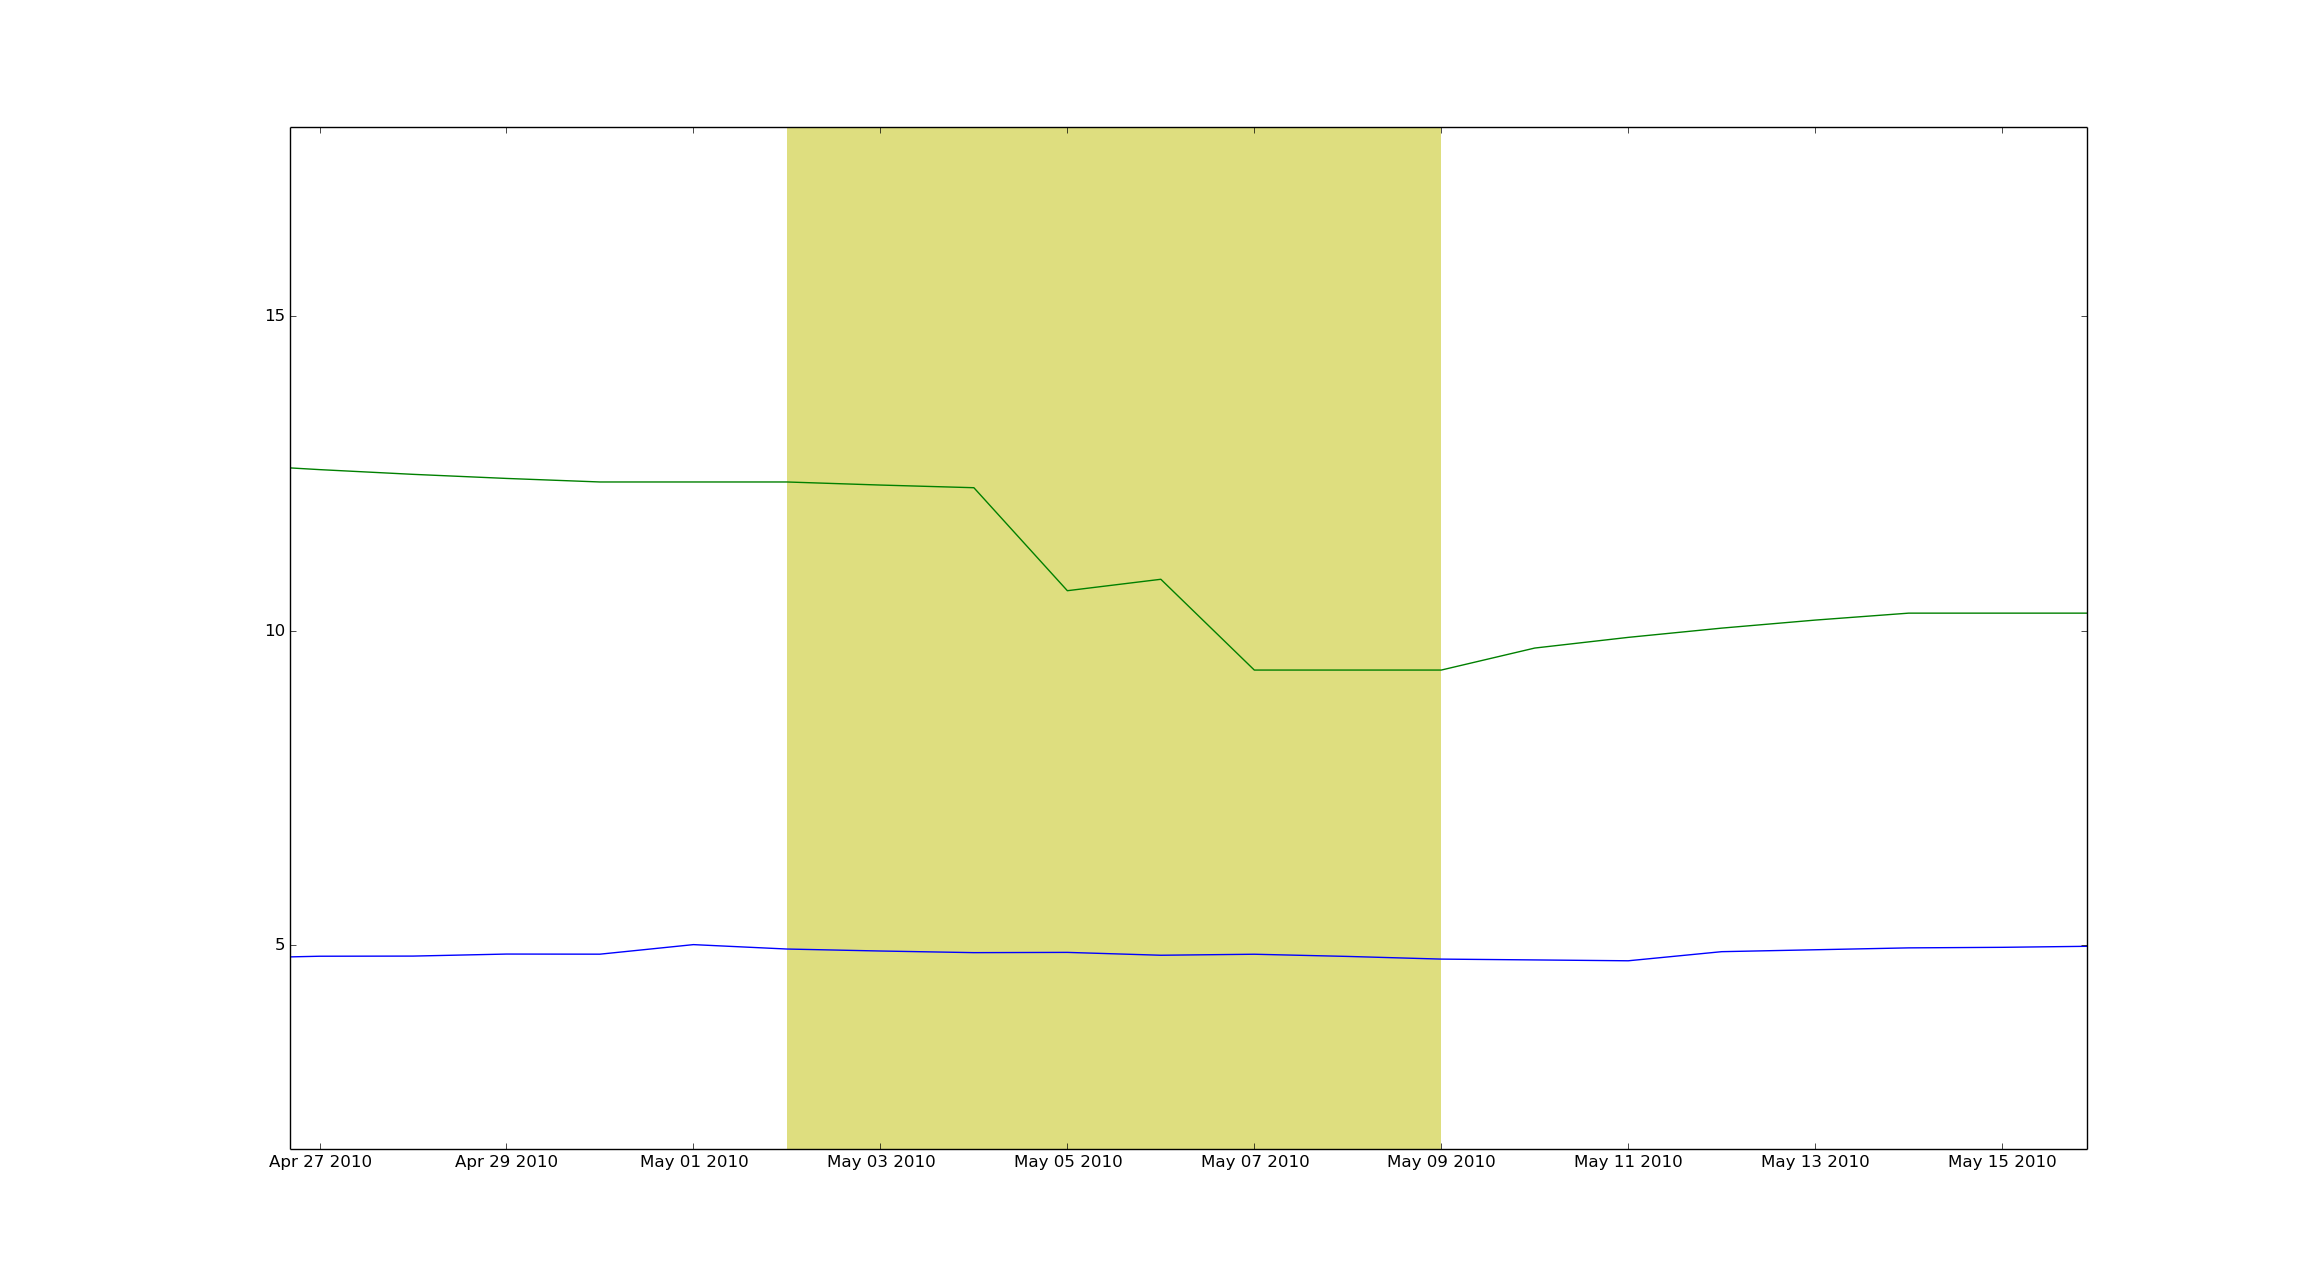
\includegraphics[width=0.8\textwidth]{graphs/12132.png}
		    	\caption{Slope Based Anomaly Detection (Green line - Retail Price, Blue Line - Wholesale Price)}
		    	\label{fig:12132}
			\end{figure}
						
			
			
			
			
			\item Other observation is related to why few anomalies were reported in news but not by our system. Reason for that is we are comparing relative change in two time series. Now for some dates, where news article is present but our system did not report, value of both time series increased together. Although, prices went too high, but still relative change, i.e. slope value remained relatively low as compared to others. So that was not reported by our system.
				
			Following tenures are some cases reported by this method:
			\begin{itemize}
				\item \textit{Analysis 1}: Dec 2010, Jan Feb 2012, June 2013, May June 2015   (See Figure \ref{fig:12113})
				\item \textit{Analysis 3}: Feb 2013, July 2014   (See Figure \ref{fig:12133})
			\end{itemize}
			
			\begin{figure}[H]
		    	\centering
  		    	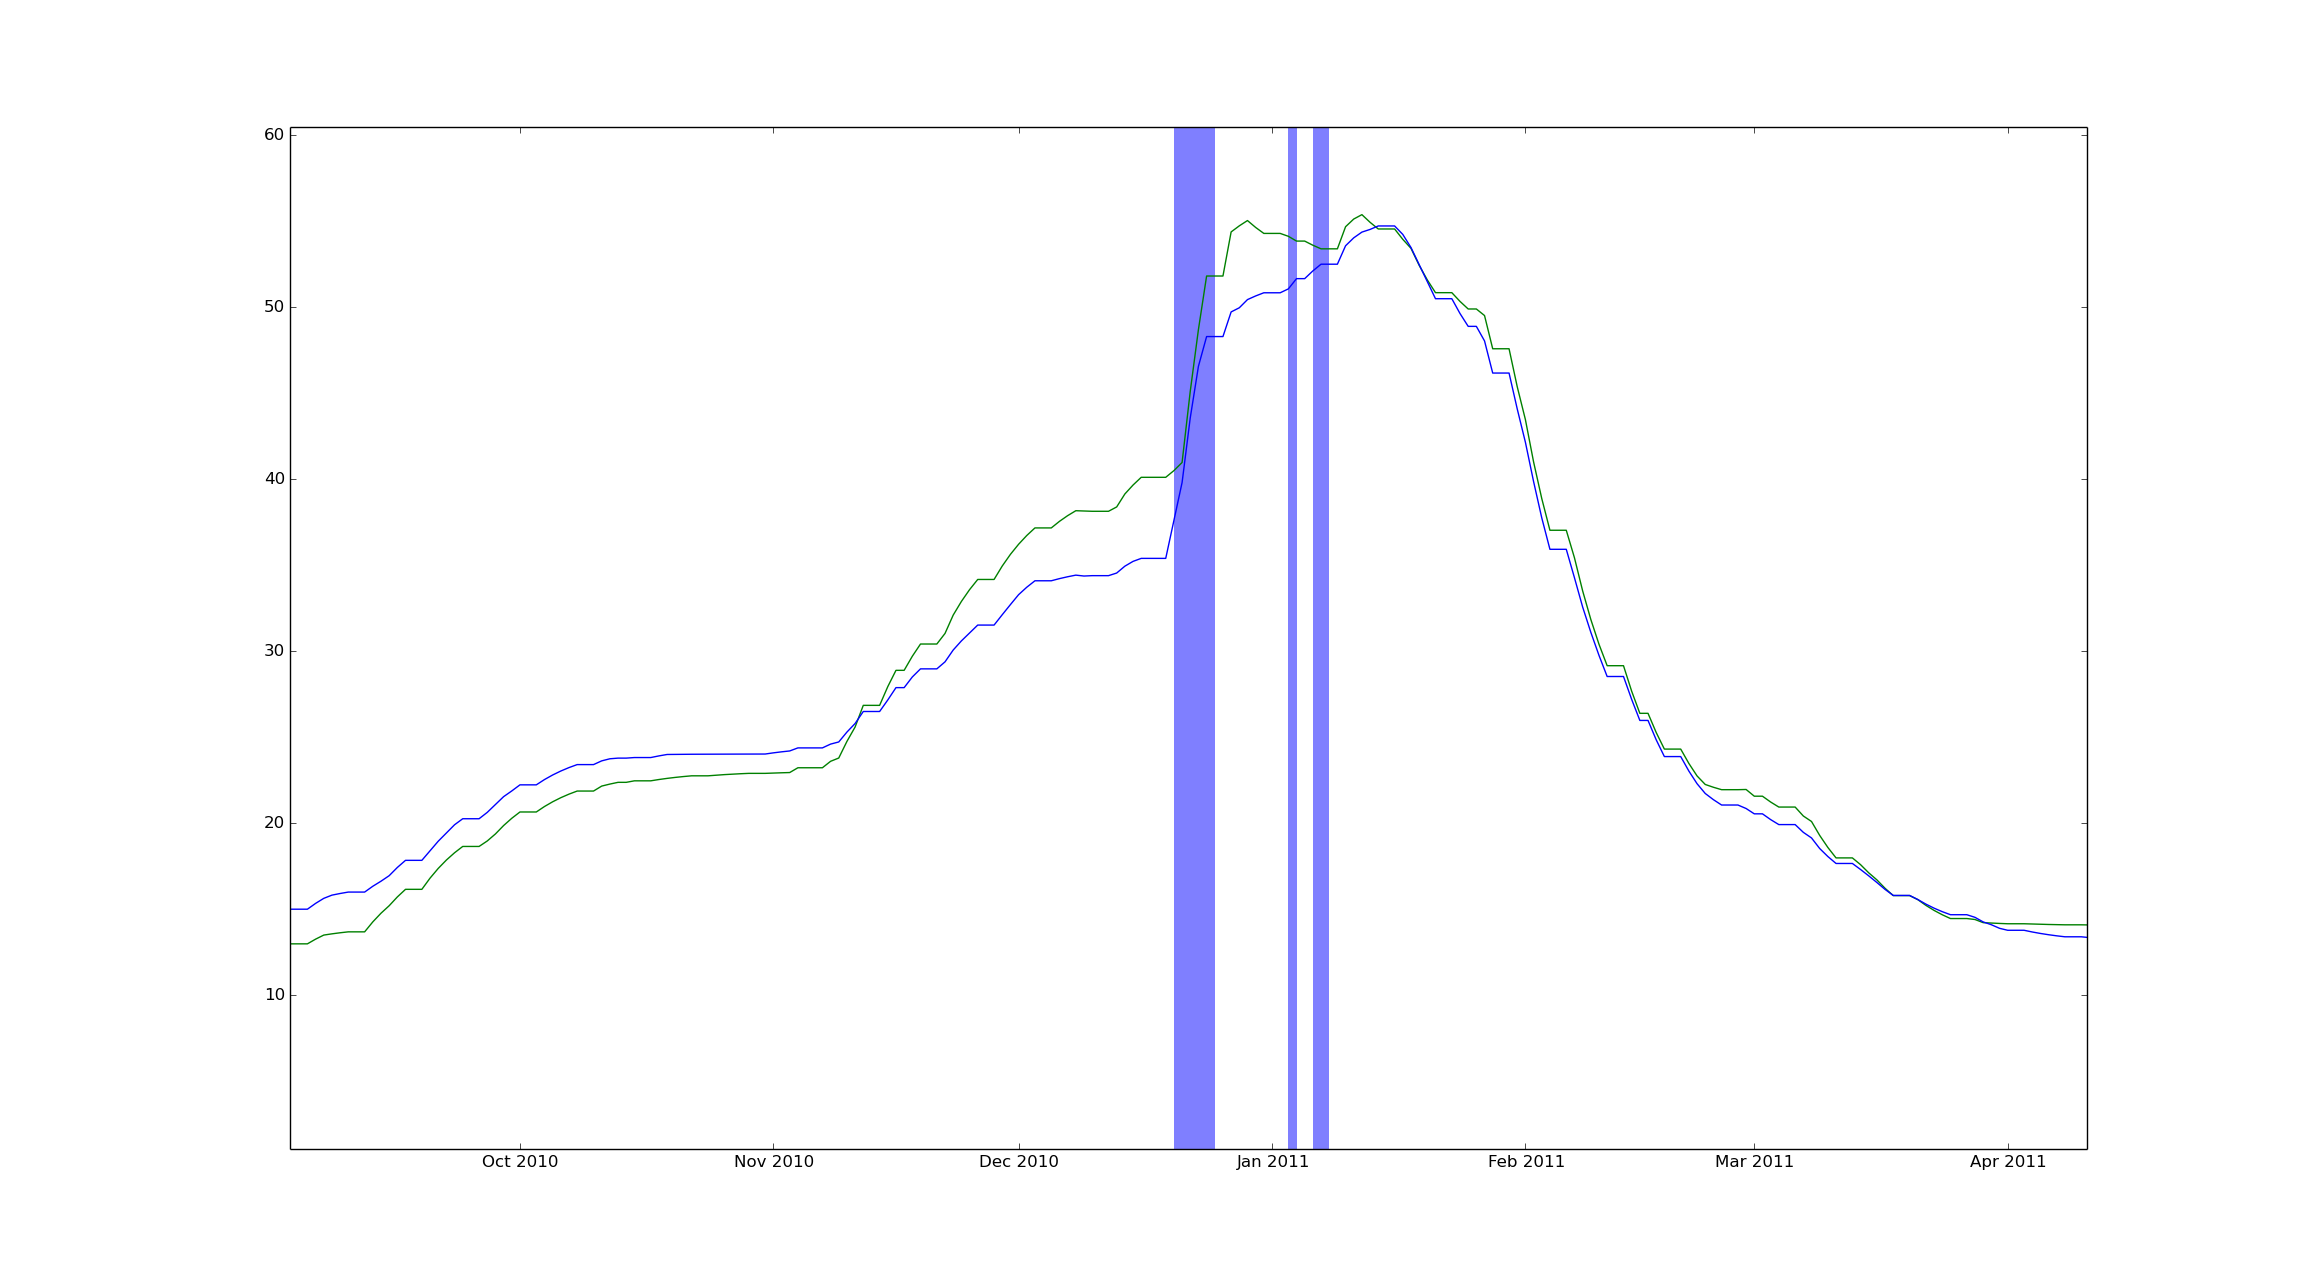
\includegraphics[width=0.8\textwidth]{graphs/12113.png}
		    	\caption{Slope Based Anomaly Detection (Green line - Centre Retail Price, Blue Line - Average Retail Price)}
		    	\label{fig:12113}
			\end{figure}
			
			\begin{figure}[H]
		    	\centering
  		    	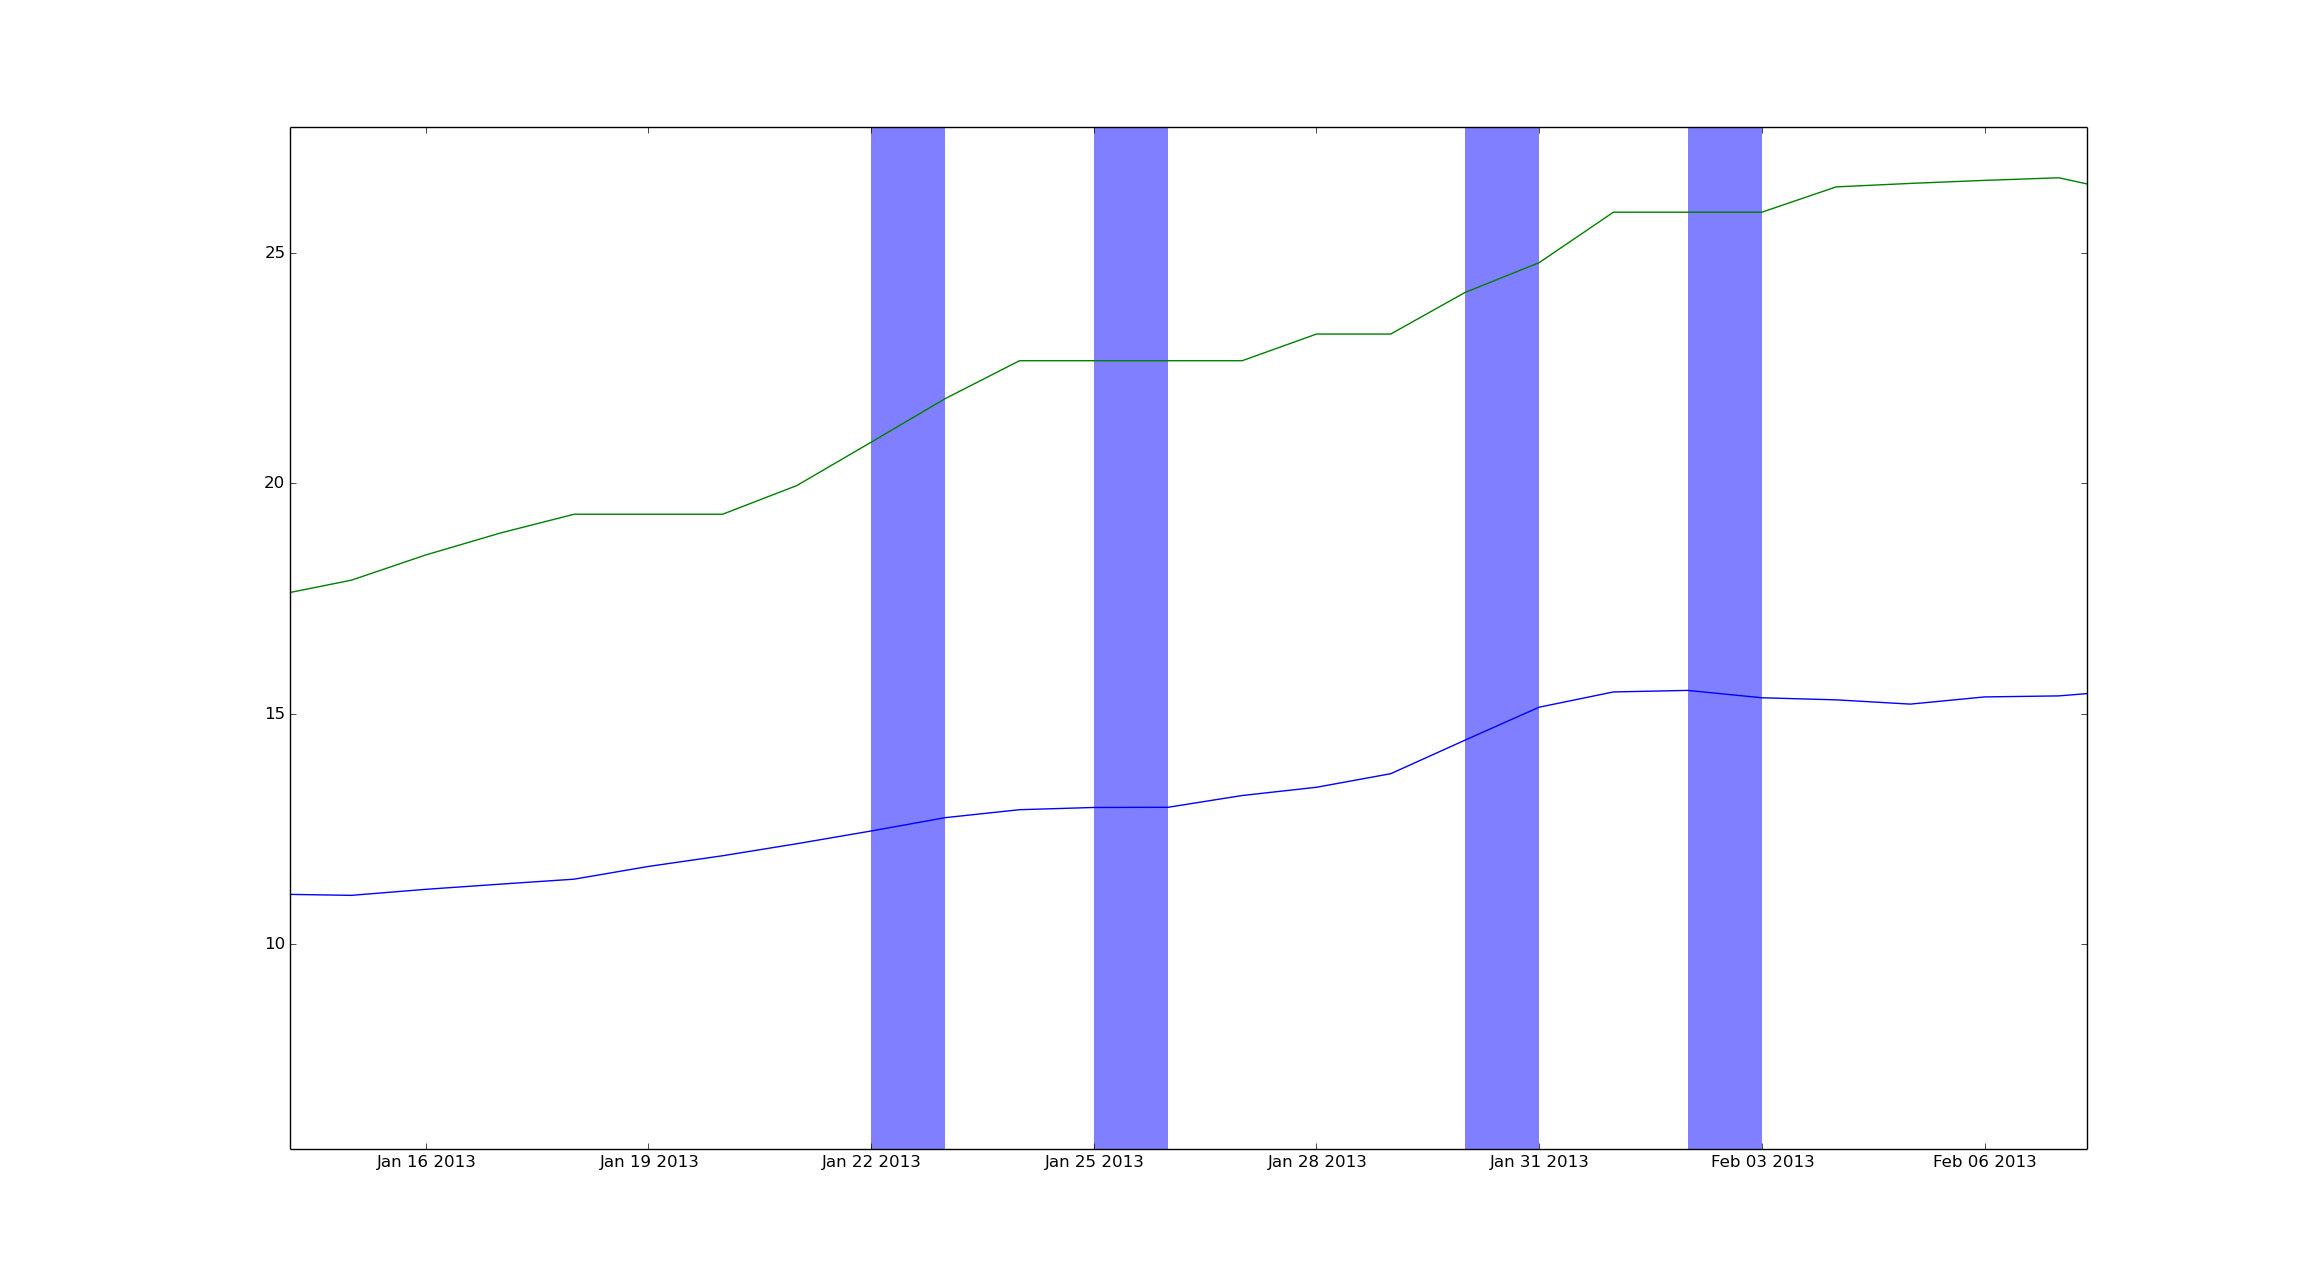
\includegraphics[width=0.8\textwidth]{graphs/12133.png}
		    	\caption{Slope Based Anomaly Detection (Green line - Retail Price, Blue Line - Wholesale Price)}
		    	\label{fig:12133}
			\end{figure}
			
			\item In some cases, original retail price was running less than average retail price for some time and then suddenly prices in the centre increased drastically. So such cases were reported as anomaly in this method, which is quite normal. Such cases were found in \textit{Analysis 1} for Nov 2011, Feb Mar 2012 and Dec 2014. (See Figure \ref{fig:12114})
			
			\begin{figure}[H]
		    	\centering
  		    	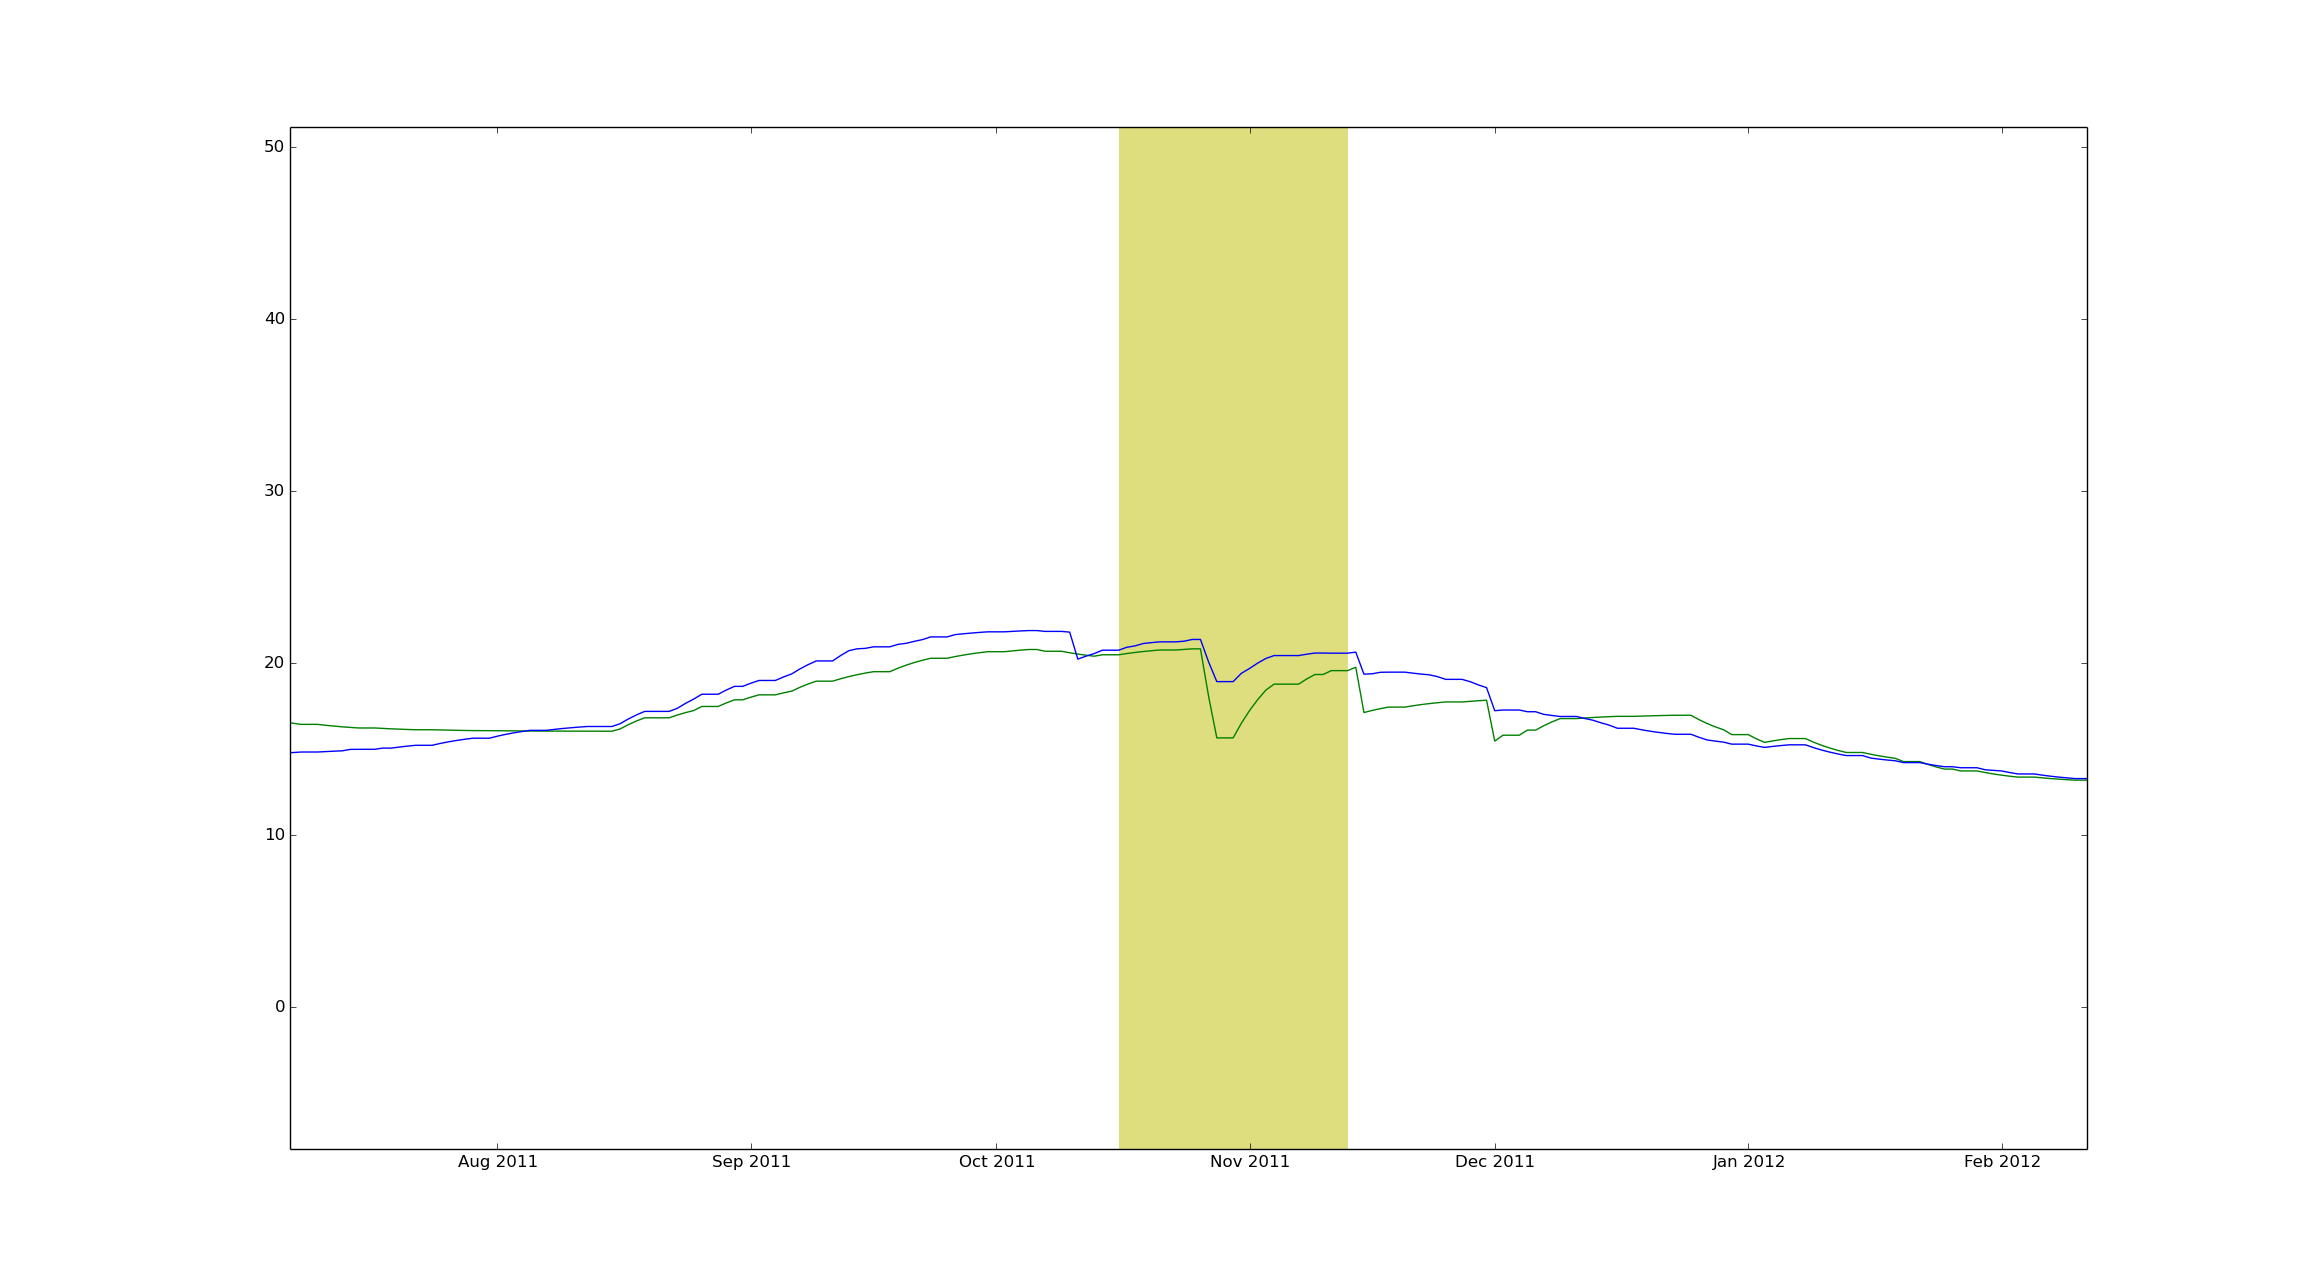
\includegraphics[width=0.8\textwidth]{graphs/12114.png}
		    	\caption{Slope Based Anomaly Detection (Green line - Centre Retail Price, Blue Line - Average Retail Price)}
		    	\label{fig:12114}
			\end{figure}			
			
			\item In some cases, tenure reported as anomaly is quite large, because situations were abnormal for long time. But is not necessary that news articles should be present for such a large tenure and anomaly reported was justifiable. For\textit{ Analysis 1}, such tenure was reported for March end to May start 2014.  (See Figure \ref{fig:12115})
			
			\begin{figure}[H]
		    	\centering
  		    	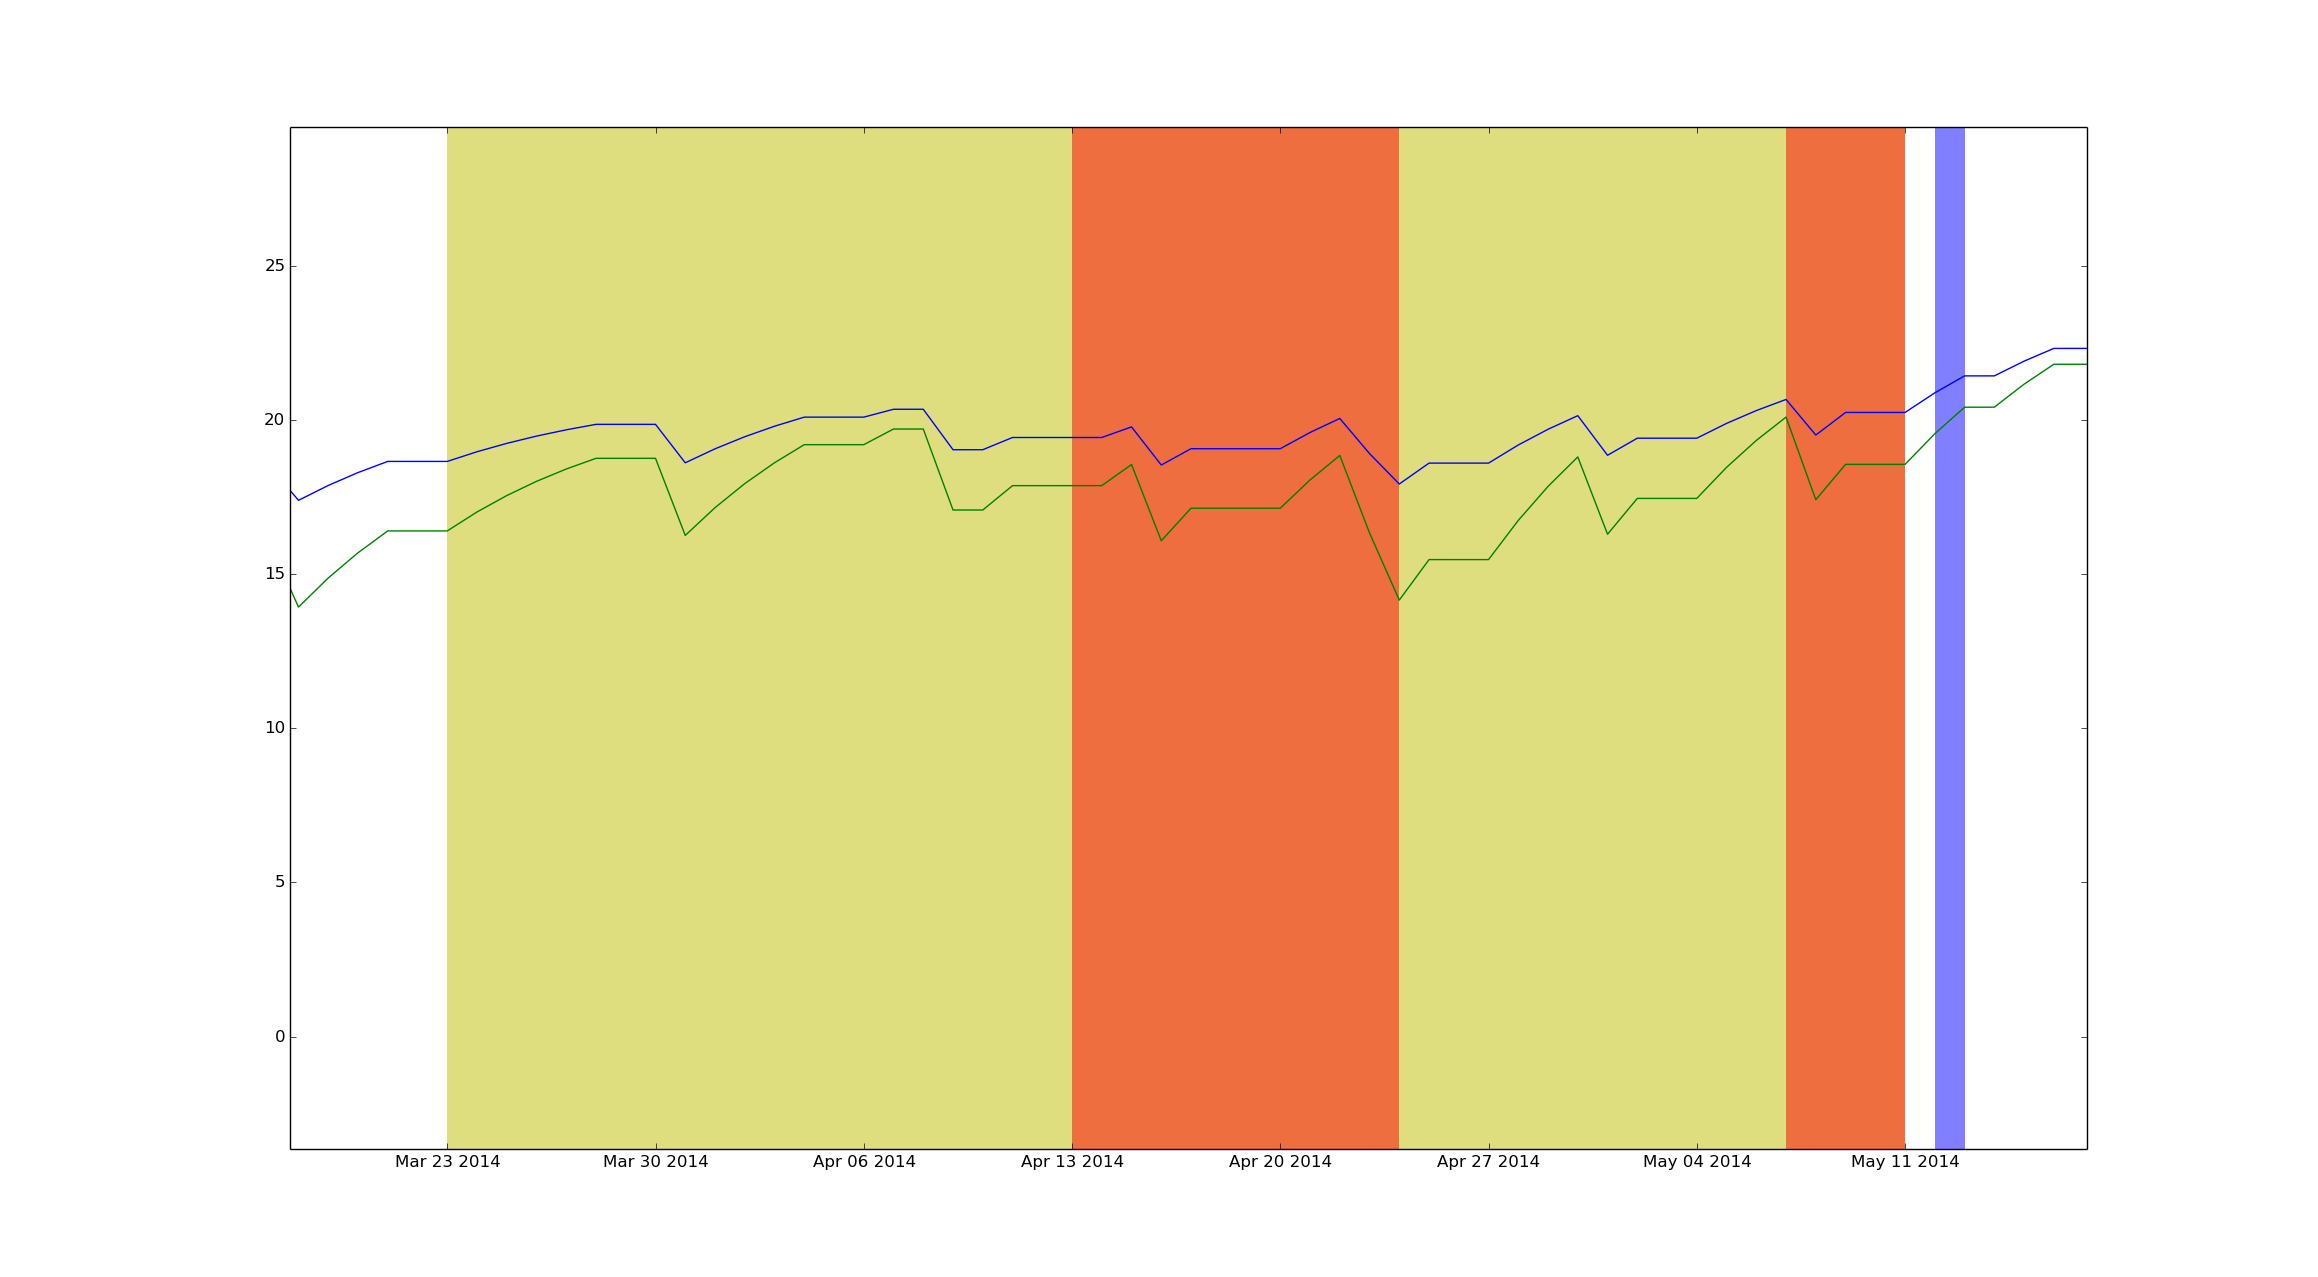
\includegraphics[width=0.8\textwidth]{graphs/12115.png}
		    	\caption{Slope Based Anomaly Detection (Green line - Centre Retail Price, Blue Line - Average Retail Price)}
		    	\label{fig:12115}
			\end{figure}			
			
			\item In \textit{Analysis 1} for June 2014, method has reported tenure upto mid June when prices started increasing but it remained high and due to that some news articles are present around June 21. We have missed because at that time relative slope value became normal. But since prices were high, it was covered by news articles. (See Figure \ref{fig:12116})
			
			\begin{figure}[H]
		    	\centering
  		    	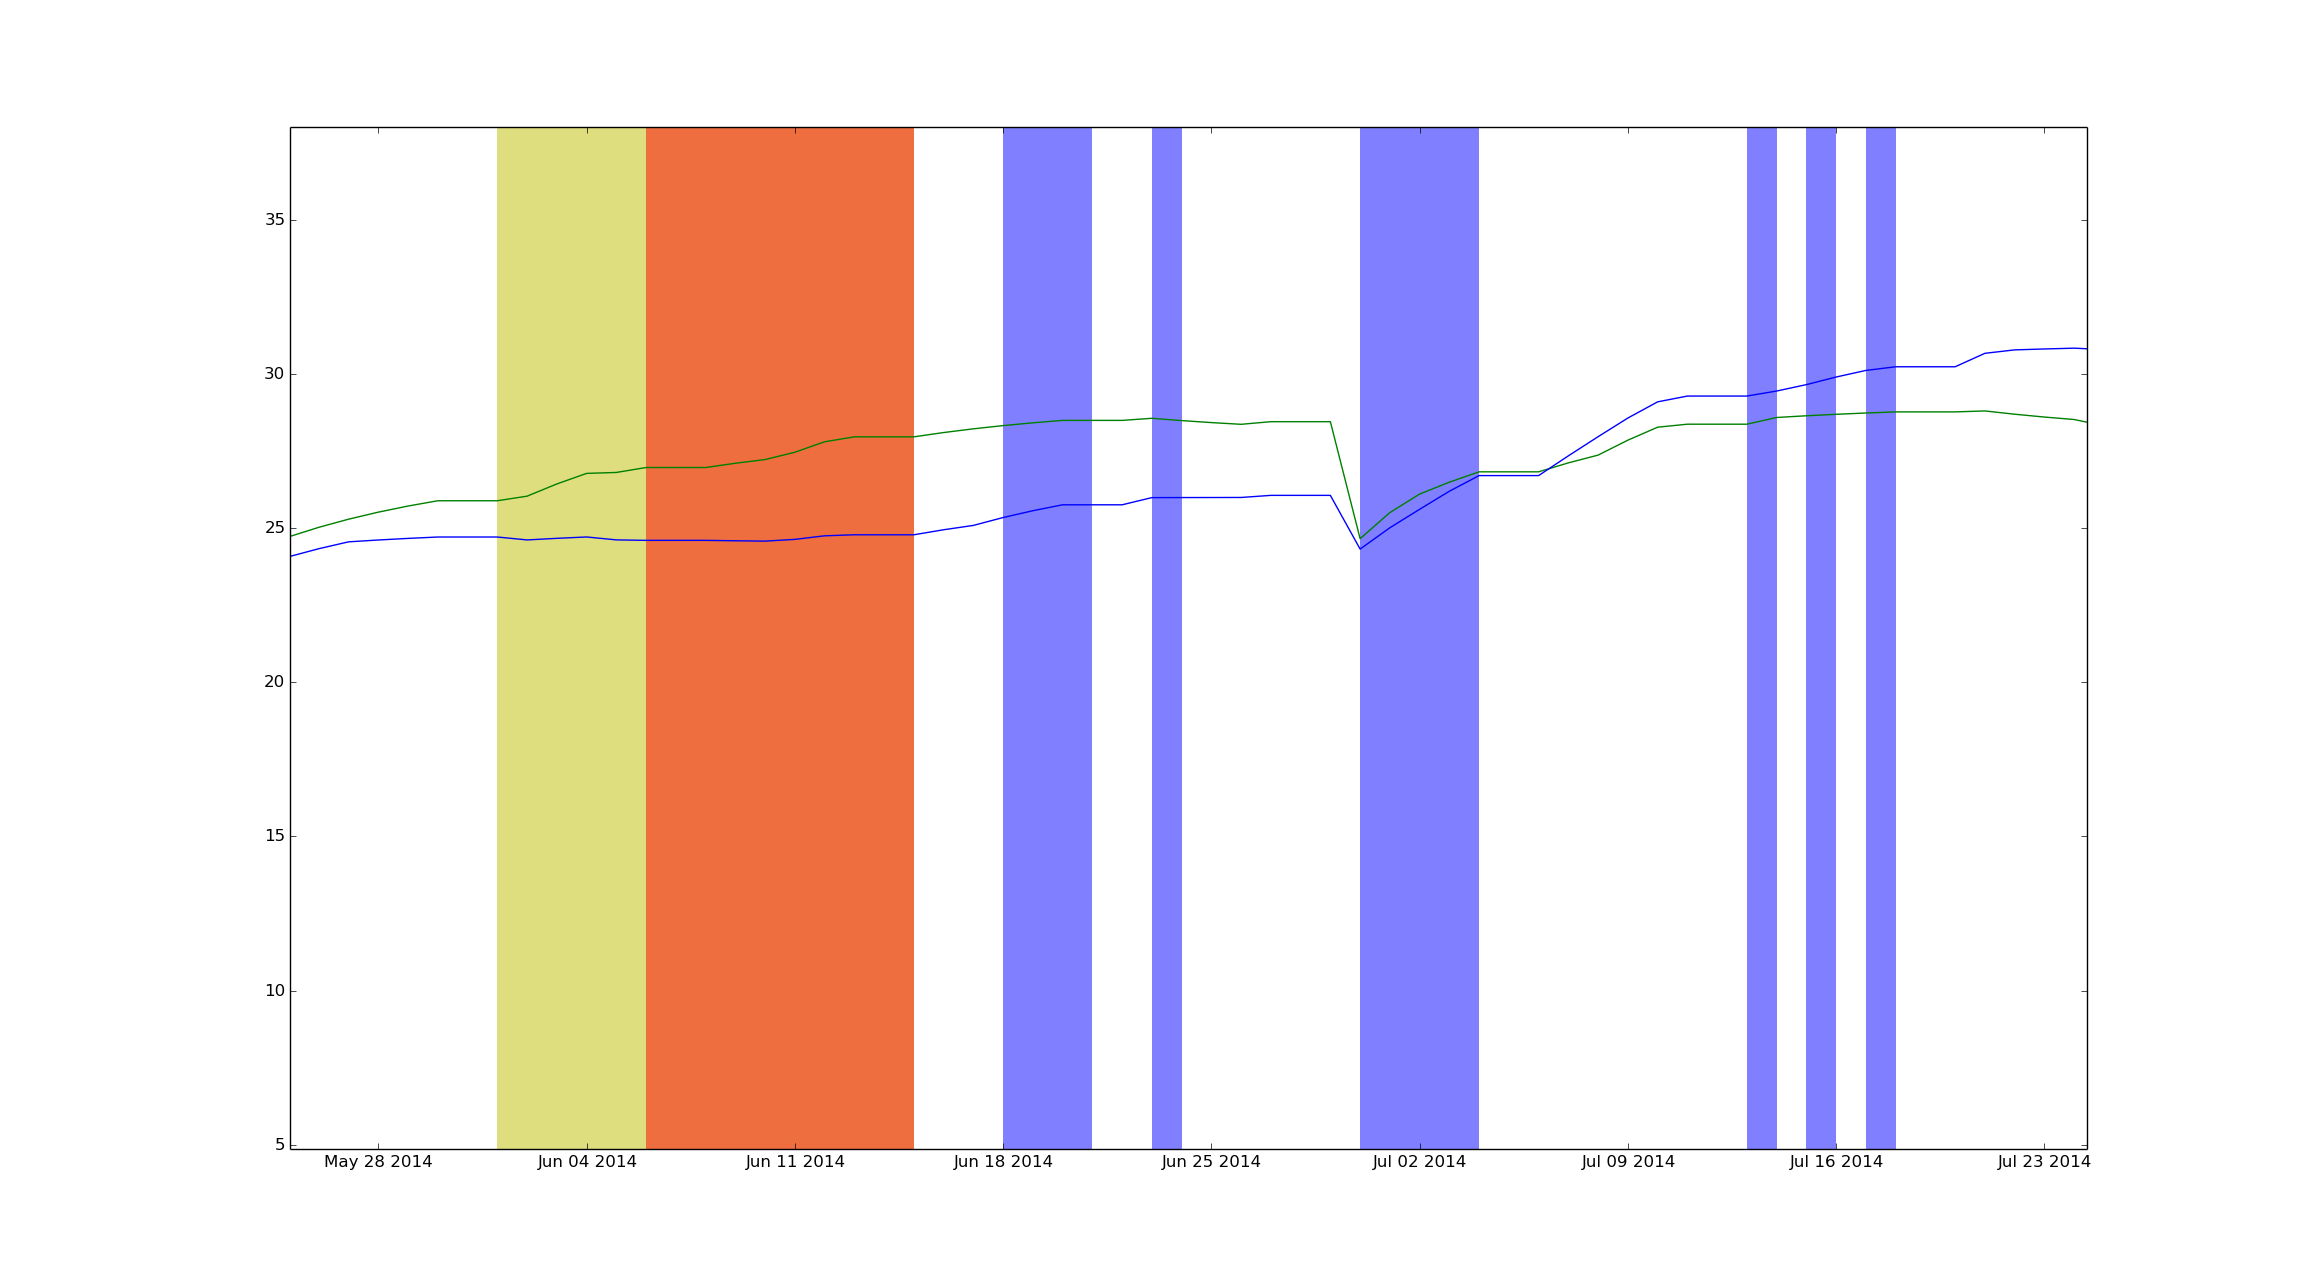
\includegraphics[width=0.8\textwidth]{graphs/12116.png}
		    	\caption{Slope Based Anomaly Detection (Green line - Centre Retail Price, Blue Line - Average Retail Price)}
		    	\label{fig:12116}
			\end{figure}			
			
			
			\item There exist some cases in \textit{Analysis 3} where retail price were decreasing but wholesale price kept on increasing, this created negative slope value, whereas in this scenario, we were looking for only positive slopes and that's why this method missed it. Such periods were in July Aug Sept 2013, Nov Dec 2013. (See Figure \ref{fig:12134})
			
			\begin{figure}[H]
		    	\centering
  		    	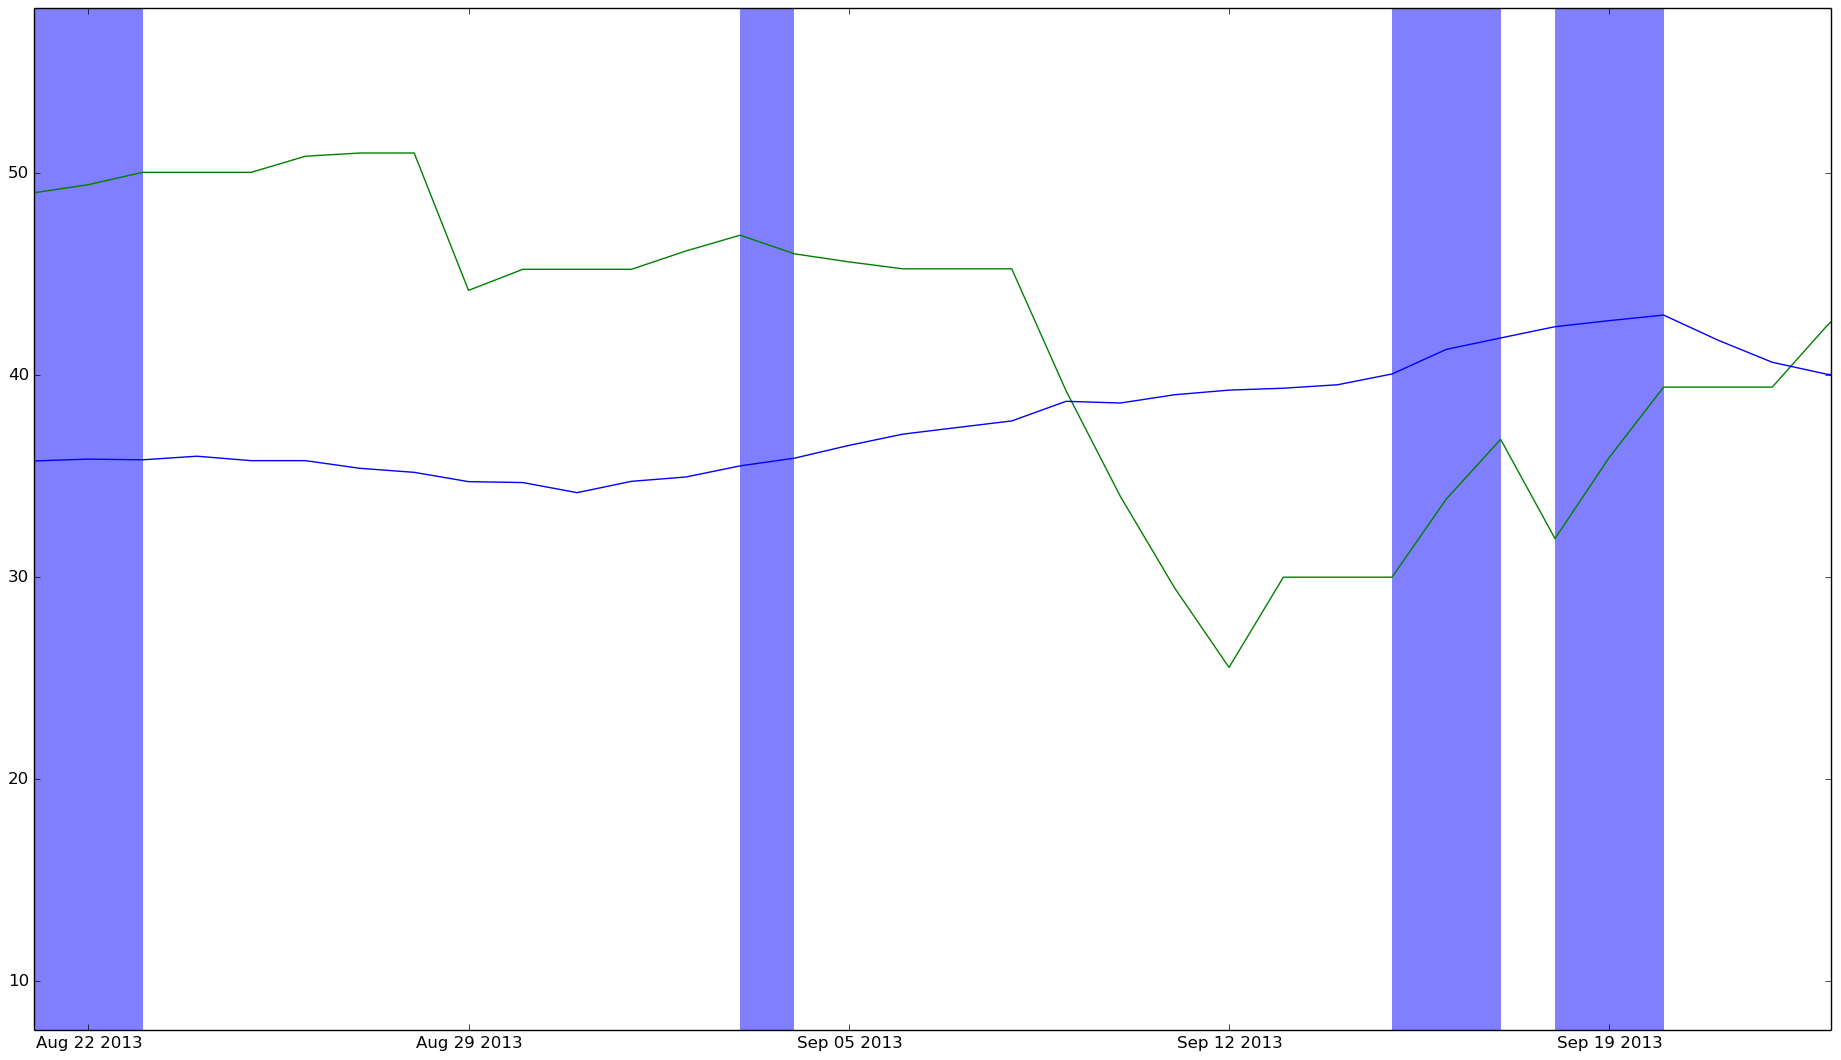
\includegraphics[width=0.8\textwidth]{graphs/12134.png}
		    	\caption{Slope Based Anomaly Detection (Green line - Retail Price, Blue Line - Wholesale Price)}
		    	\label{fig:12134}
			\end{figure}			
			
		\end{itemize}
		
		
		Now we present few observation for Analysis 2 and 4.
		
		\begin{itemize}
			\item If change in retail price or change in wholesale price is more as compared to change in arrival (prices went too high, even for small drop in arrival), then it is reported as anomaly by this method.\\
			
			Following tenures are some cases reported by this method:
			\begin{itemize}
				\item \textit{Analysis 2}: Oct Dec 2010, May Jun 2013 (See Figure \ref{fig:12121})
				\item \textit{Analysis 4}: Sept Oct Nov 2010, Jun 2013, Jun 2015 (See Figure \ref{fig:12141})
			\end{itemize}	
			
			\begin{figure}[H]
		    	\centering
  		    	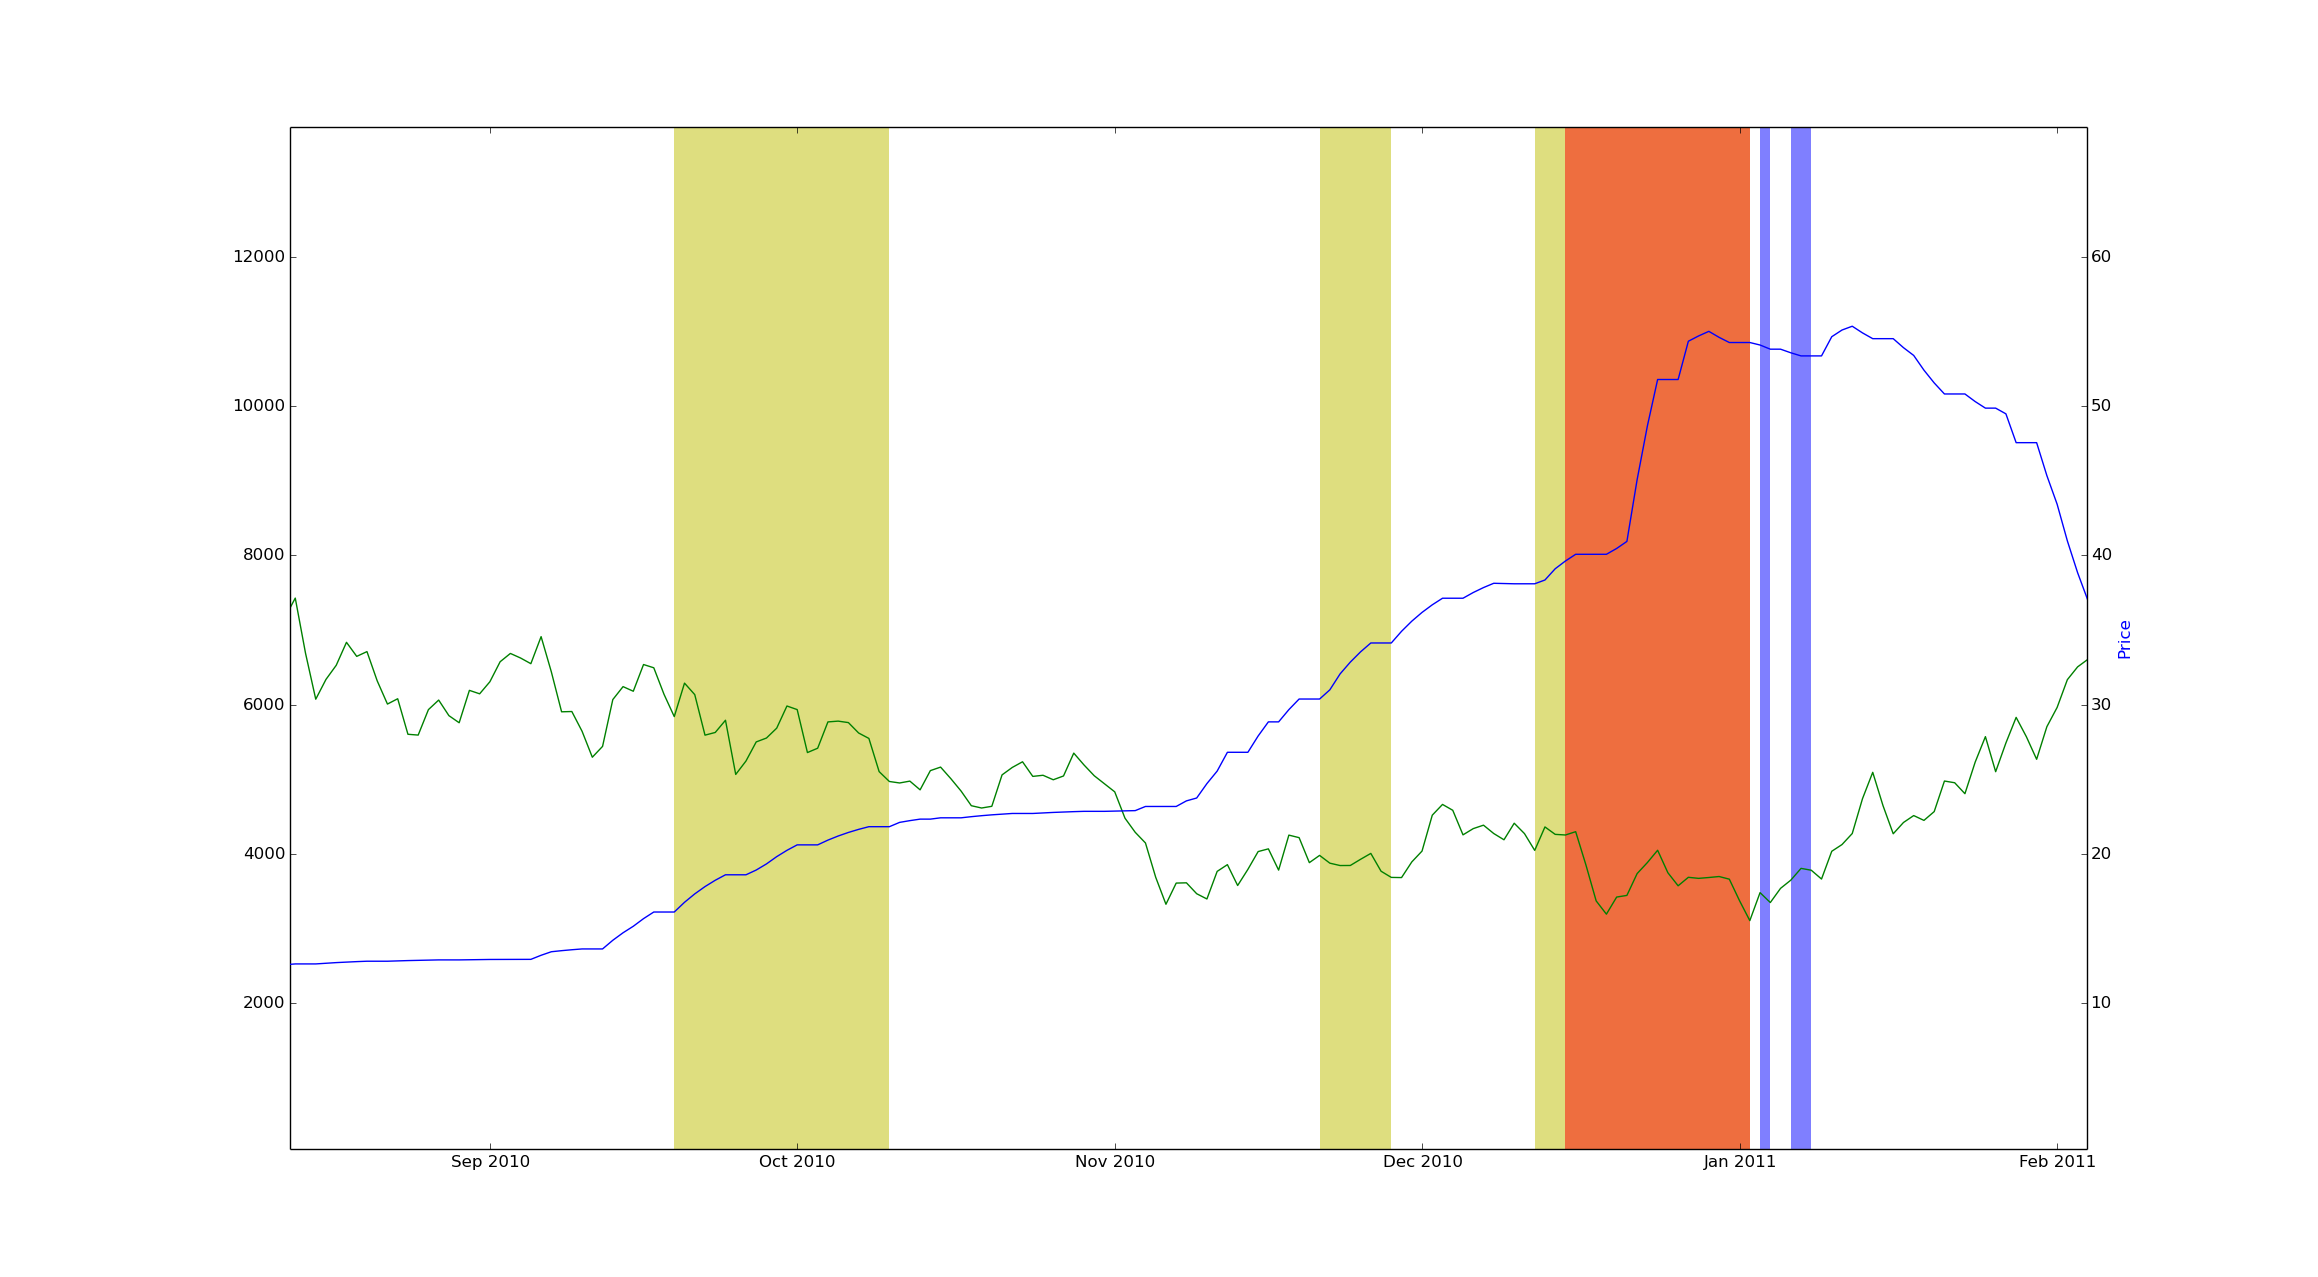
\includegraphics[width=0.8\textwidth]{graphs/12121.png}
		    	\caption{Slope Based Anomaly Detection (Green line - Arrival Data of Onion, Blue Line - Retail Price)}
		    	\label{fig:12121}
			\end{figure}
			
			\begin{figure}[H]
		    	\centering
  		    	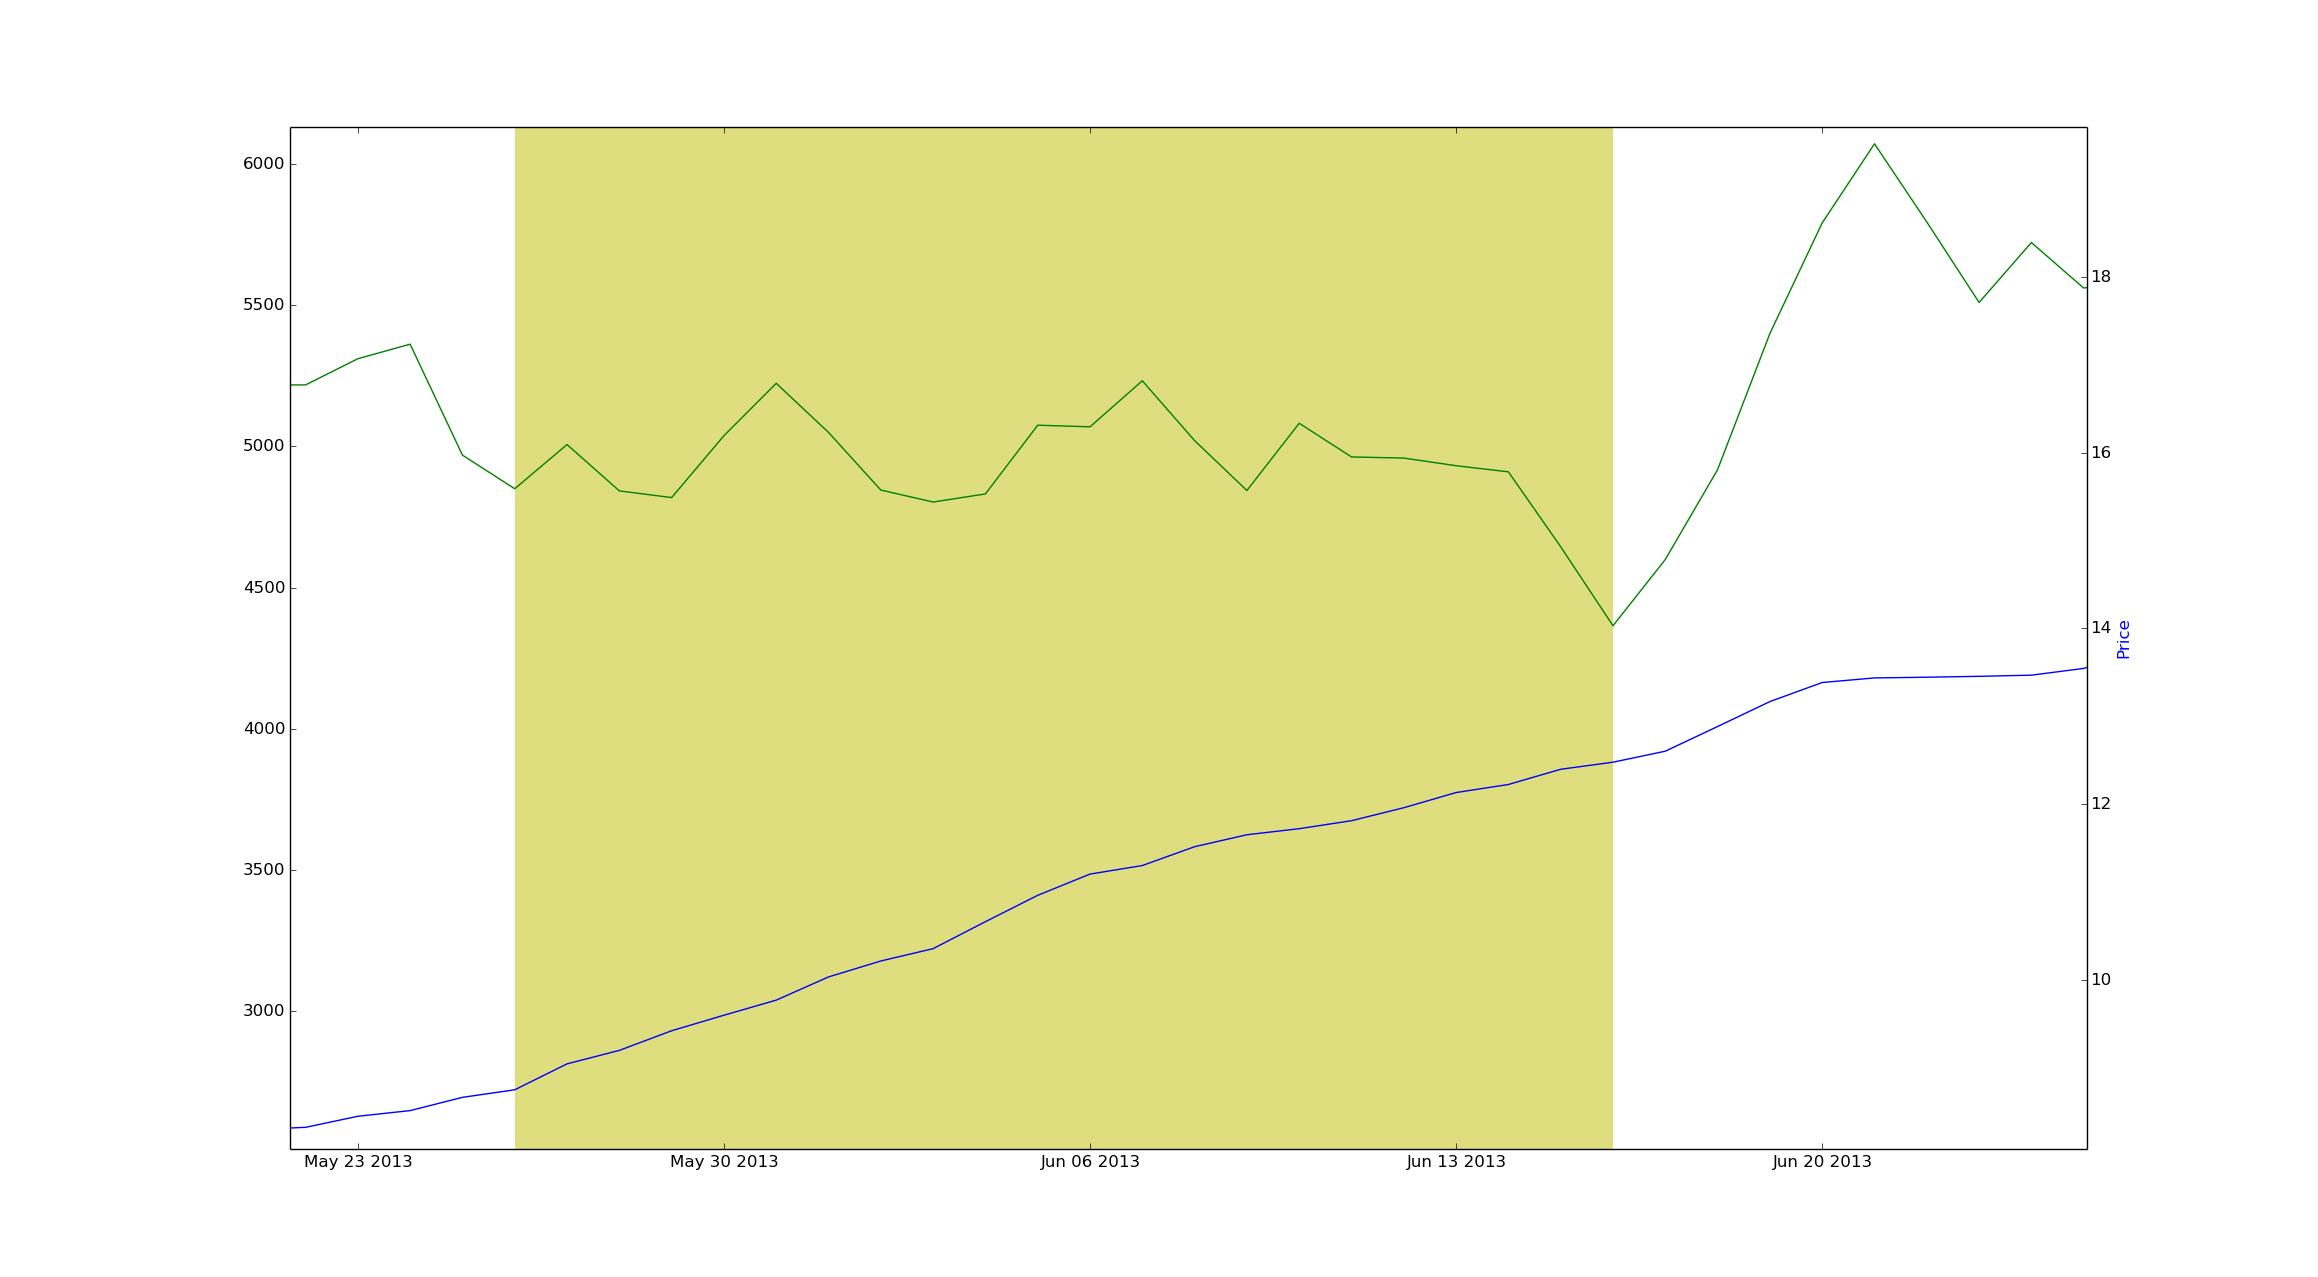
\includegraphics[width=0.8\textwidth]{graphs/12141.png}
		    	\caption{Slope Based Anomaly Detection (Green line - Arrival Data of Onion, Blue Line - Wholesale Price)}
		    	\label{fig:12141}
			\end{figure}
			
			\item But in above described scenario, when change in price is high, but prices are decreasing and when arrival is increasing, and if drop in price is too high, then also it will be reported as anomaly.	So this is limitation of this method and reports false positives in this case.\\
			Following tenures are some cases reported by this method:
			
			\begin{itemize}
				\item \textit{Analysis 2}: Feb Mar 2011, Jan Feb 2014 (See Figure \ref{fig:12122})
				\item \textit{Analysis 4}: Oct Dec 2011, Jan 2014, Mar 2011 (See Figure \ref{fig:12142})
			\end{itemize}
			
			\begin{figure}[H]
		    	\centering
  		    	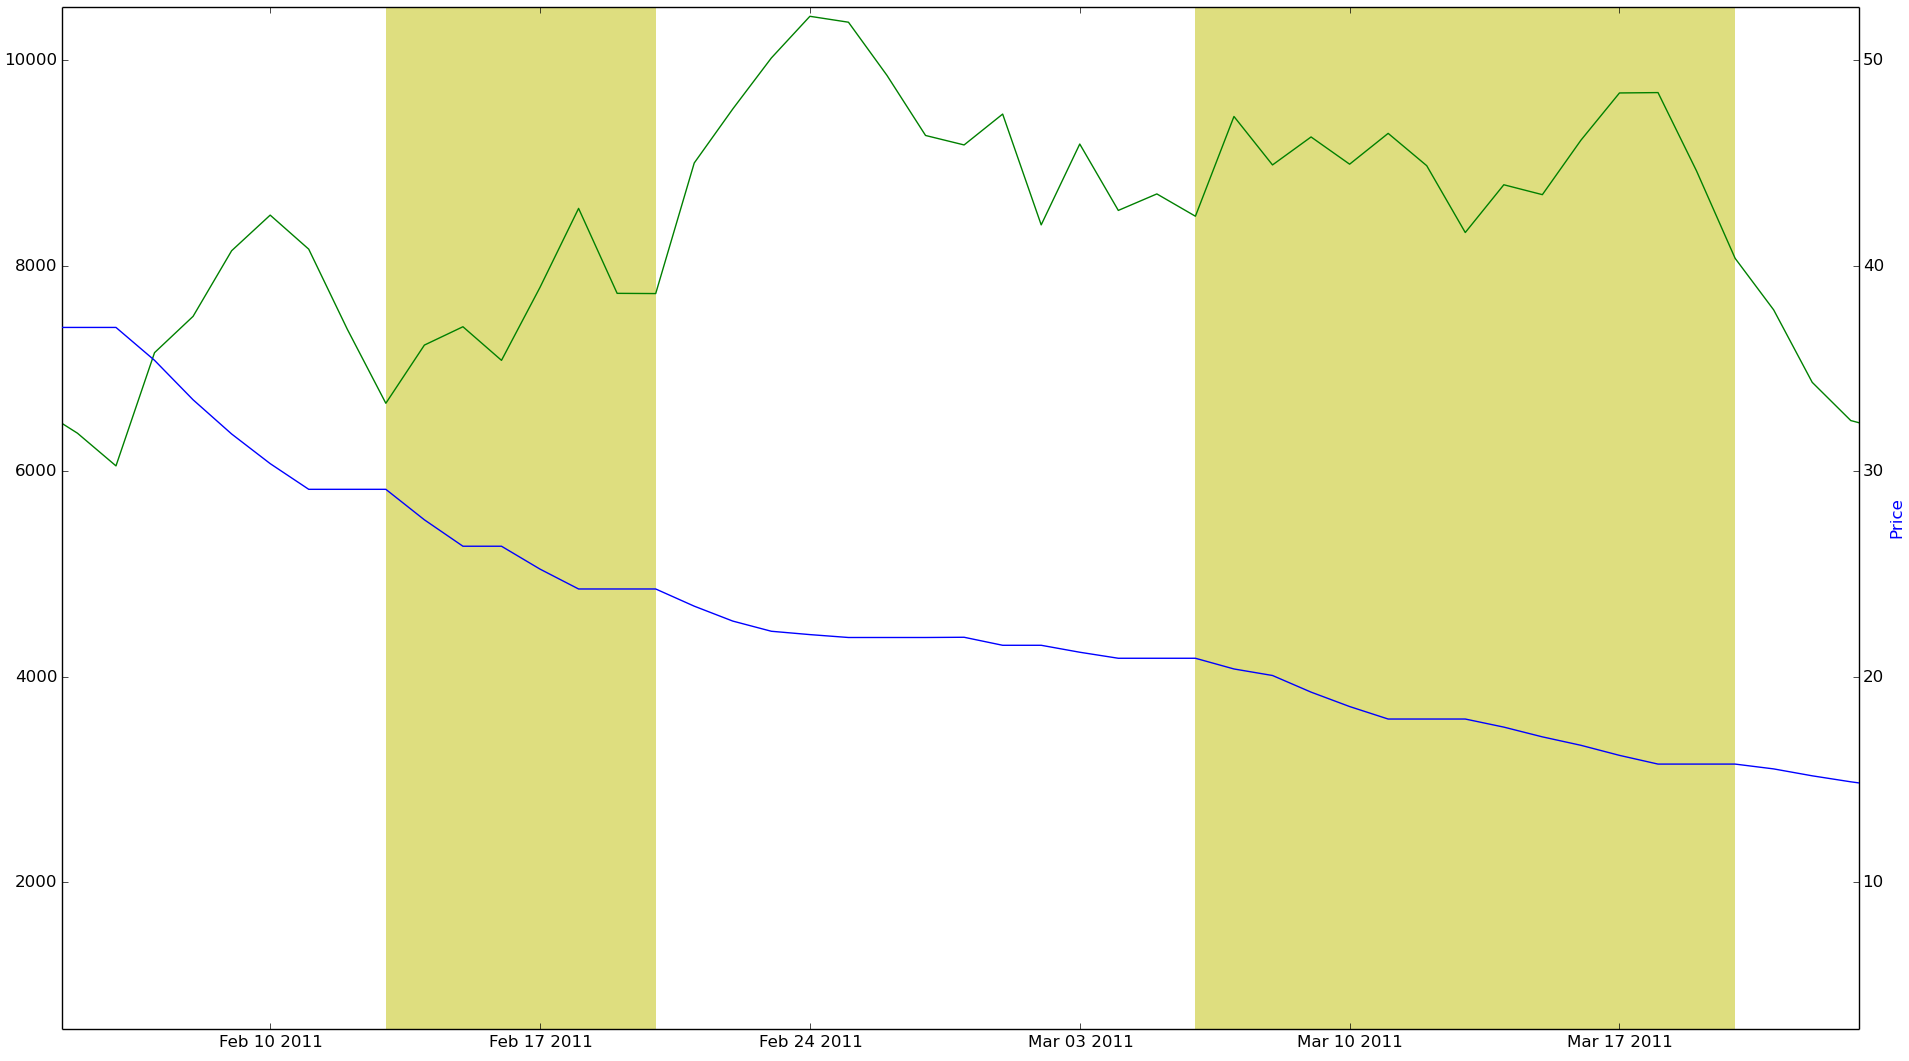
\includegraphics[width=0.8\textwidth]{graphs/12122.png}
		    	\caption{Slope Based Anomaly Detection (Green line - Arrival Data of Onion, Blue Line - Retail Price)}
		    	\label{fig:12122}
			\end{figure}
			
			\begin{figure}[H]
		    	\centering
  		    	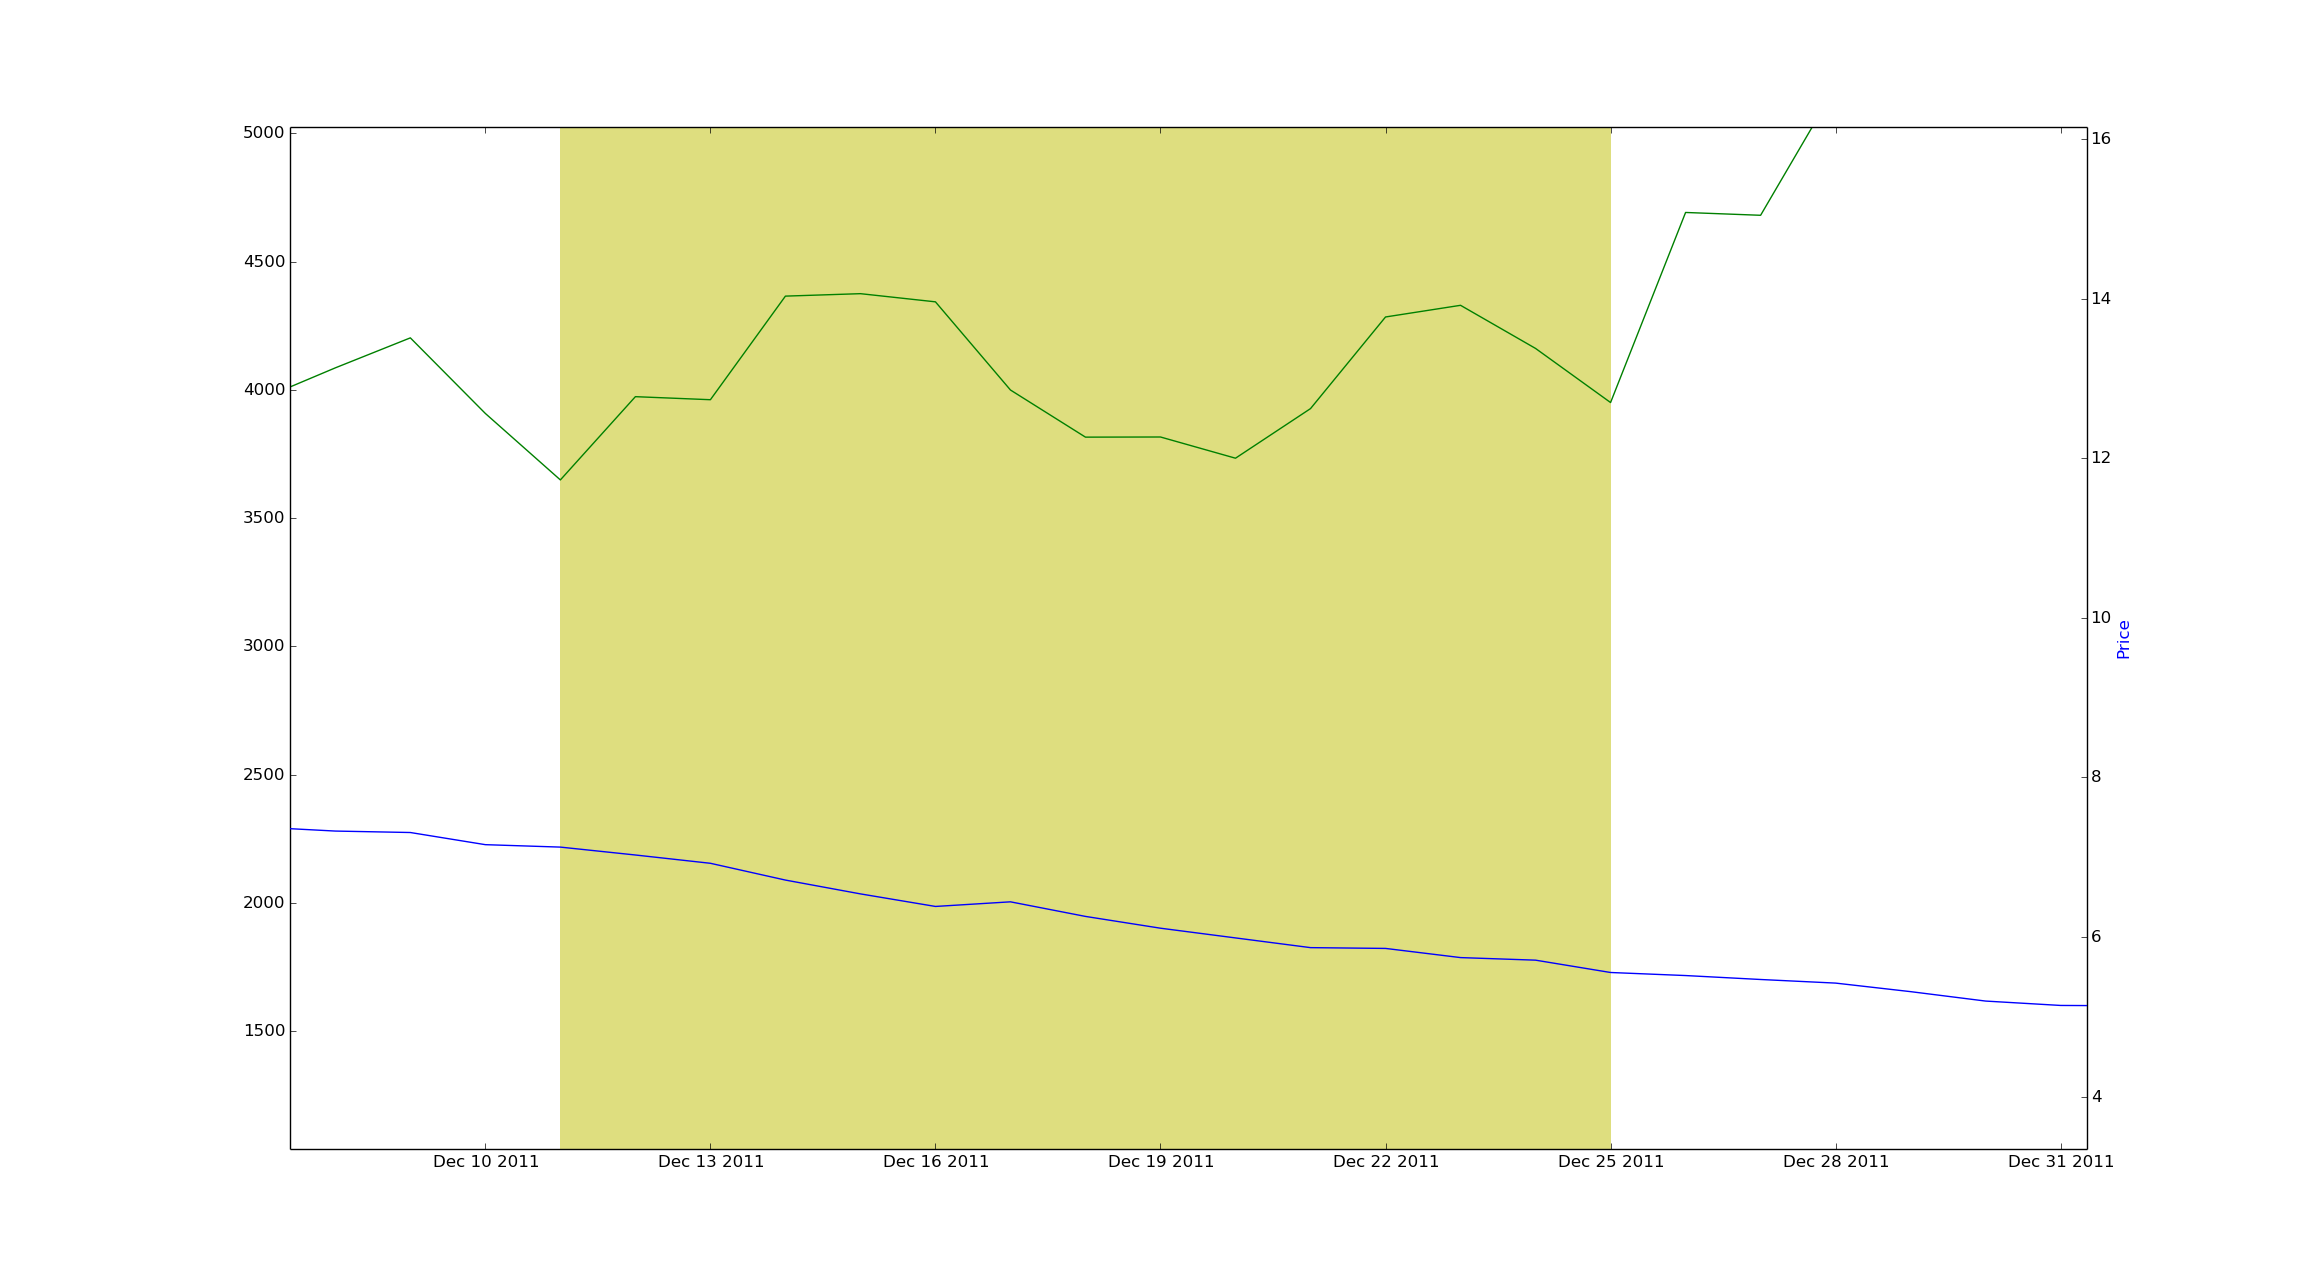
\includegraphics[width=0.8\textwidth]{graphs/12142.png}
		    	\caption{Slope Based Anomaly Detection (Green line - Arrival Data of Onion, Blue Line - Wholesale Price)}
		    	\label{fig:12142}
			\end{figure}
			
			\item One more limitation of this method is when arrival is increasing but along with that retail or wholesale price is also increasing. This will result into a positive slope and in this scenario we are only looking for negative slope and that's why, this will not be reported as anomaly and news articles corresponding to this tenure will not be matched by results of this method.\\		
			
			Following tenures are some cases reported by this method:
			\begin{itemize}
				\item \textit{Analysis 2}: Jan Feb July Nov 2013, June July 2014 (See Figure \ref{fig:12123})
				\item \textit{Analysis 4}: Jan Feb 2013, July 2014, June 2015 (See Figure \ref{fig:12143})
			\end{itemize}
			
			\begin{figure}[H]
		    	\centering
  		    	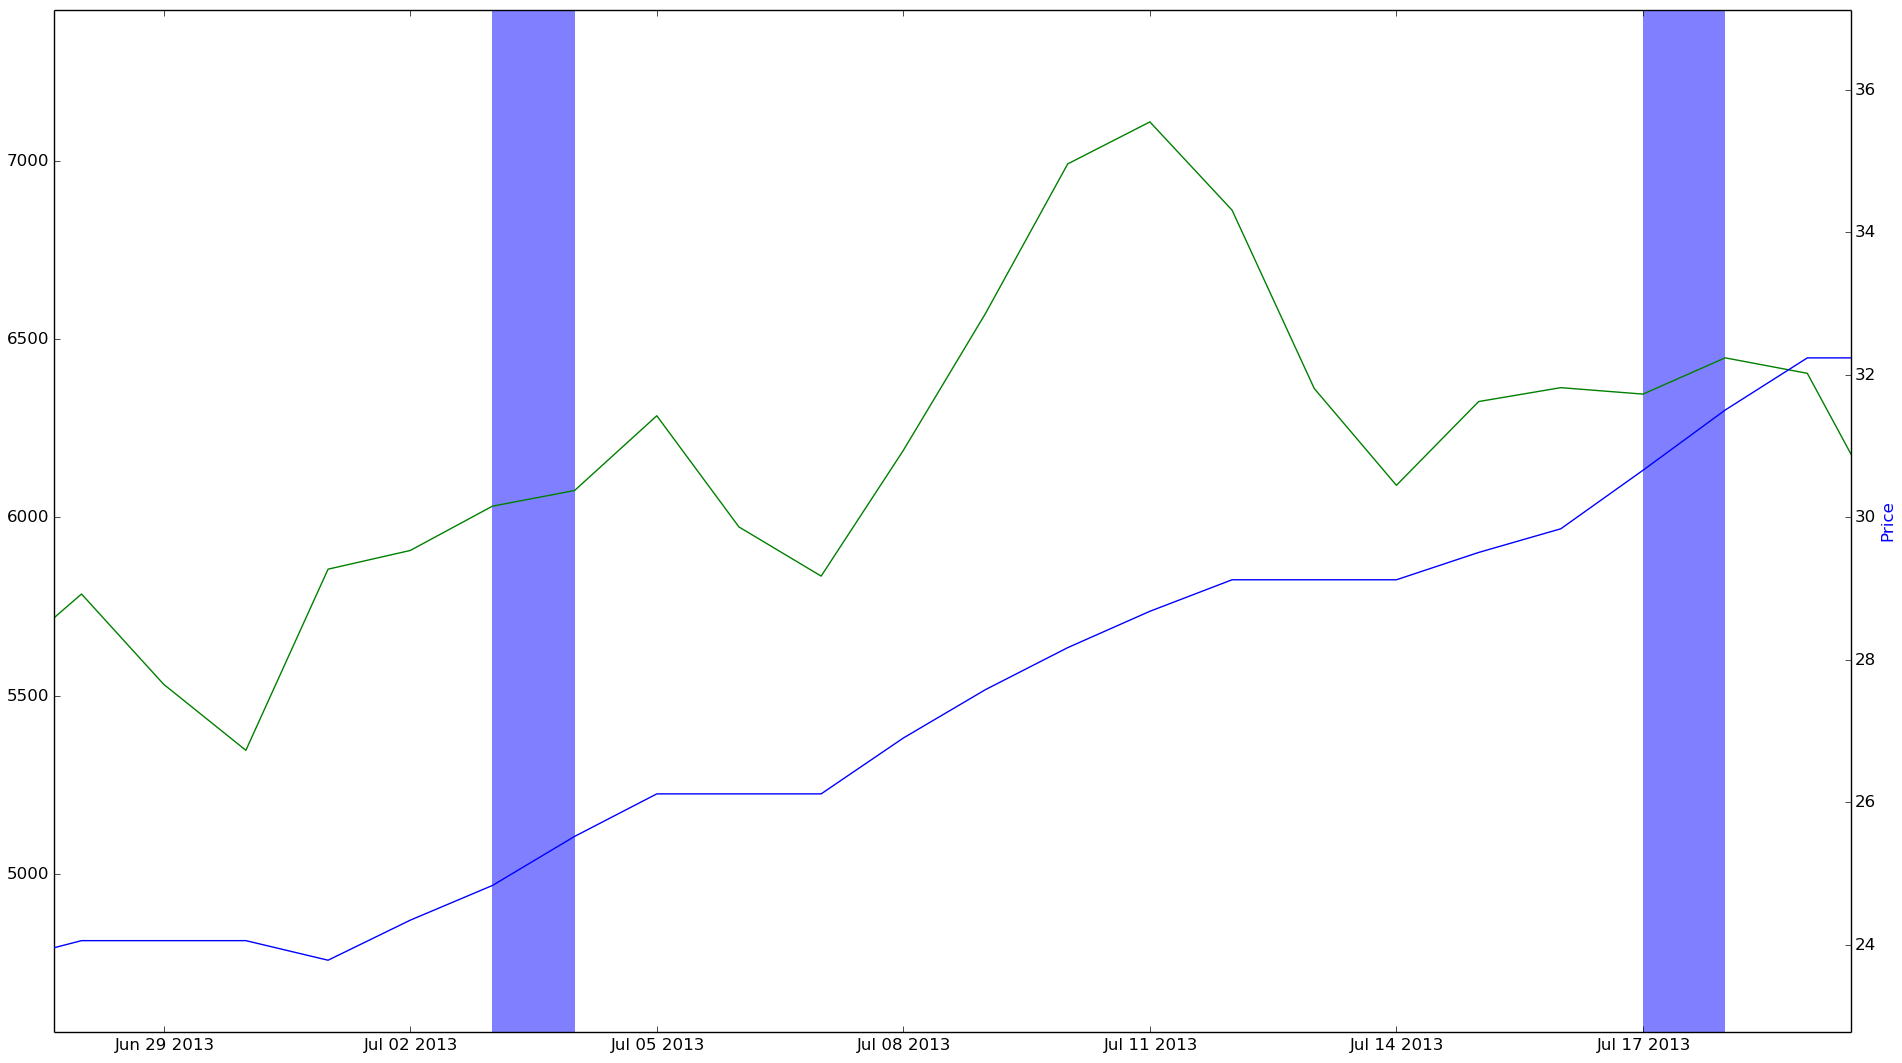
\includegraphics[width=0.8\textwidth]{graphs/12123.png}
		    	\caption{Slope Based Anomaly Detection (Green line - Arrival Data of Onion, Blue Line - Retail Price)}
		    	\label{fig:12123}
			\end{figure}
			
			\begin{figure}[H]
		    	\centering
  		    	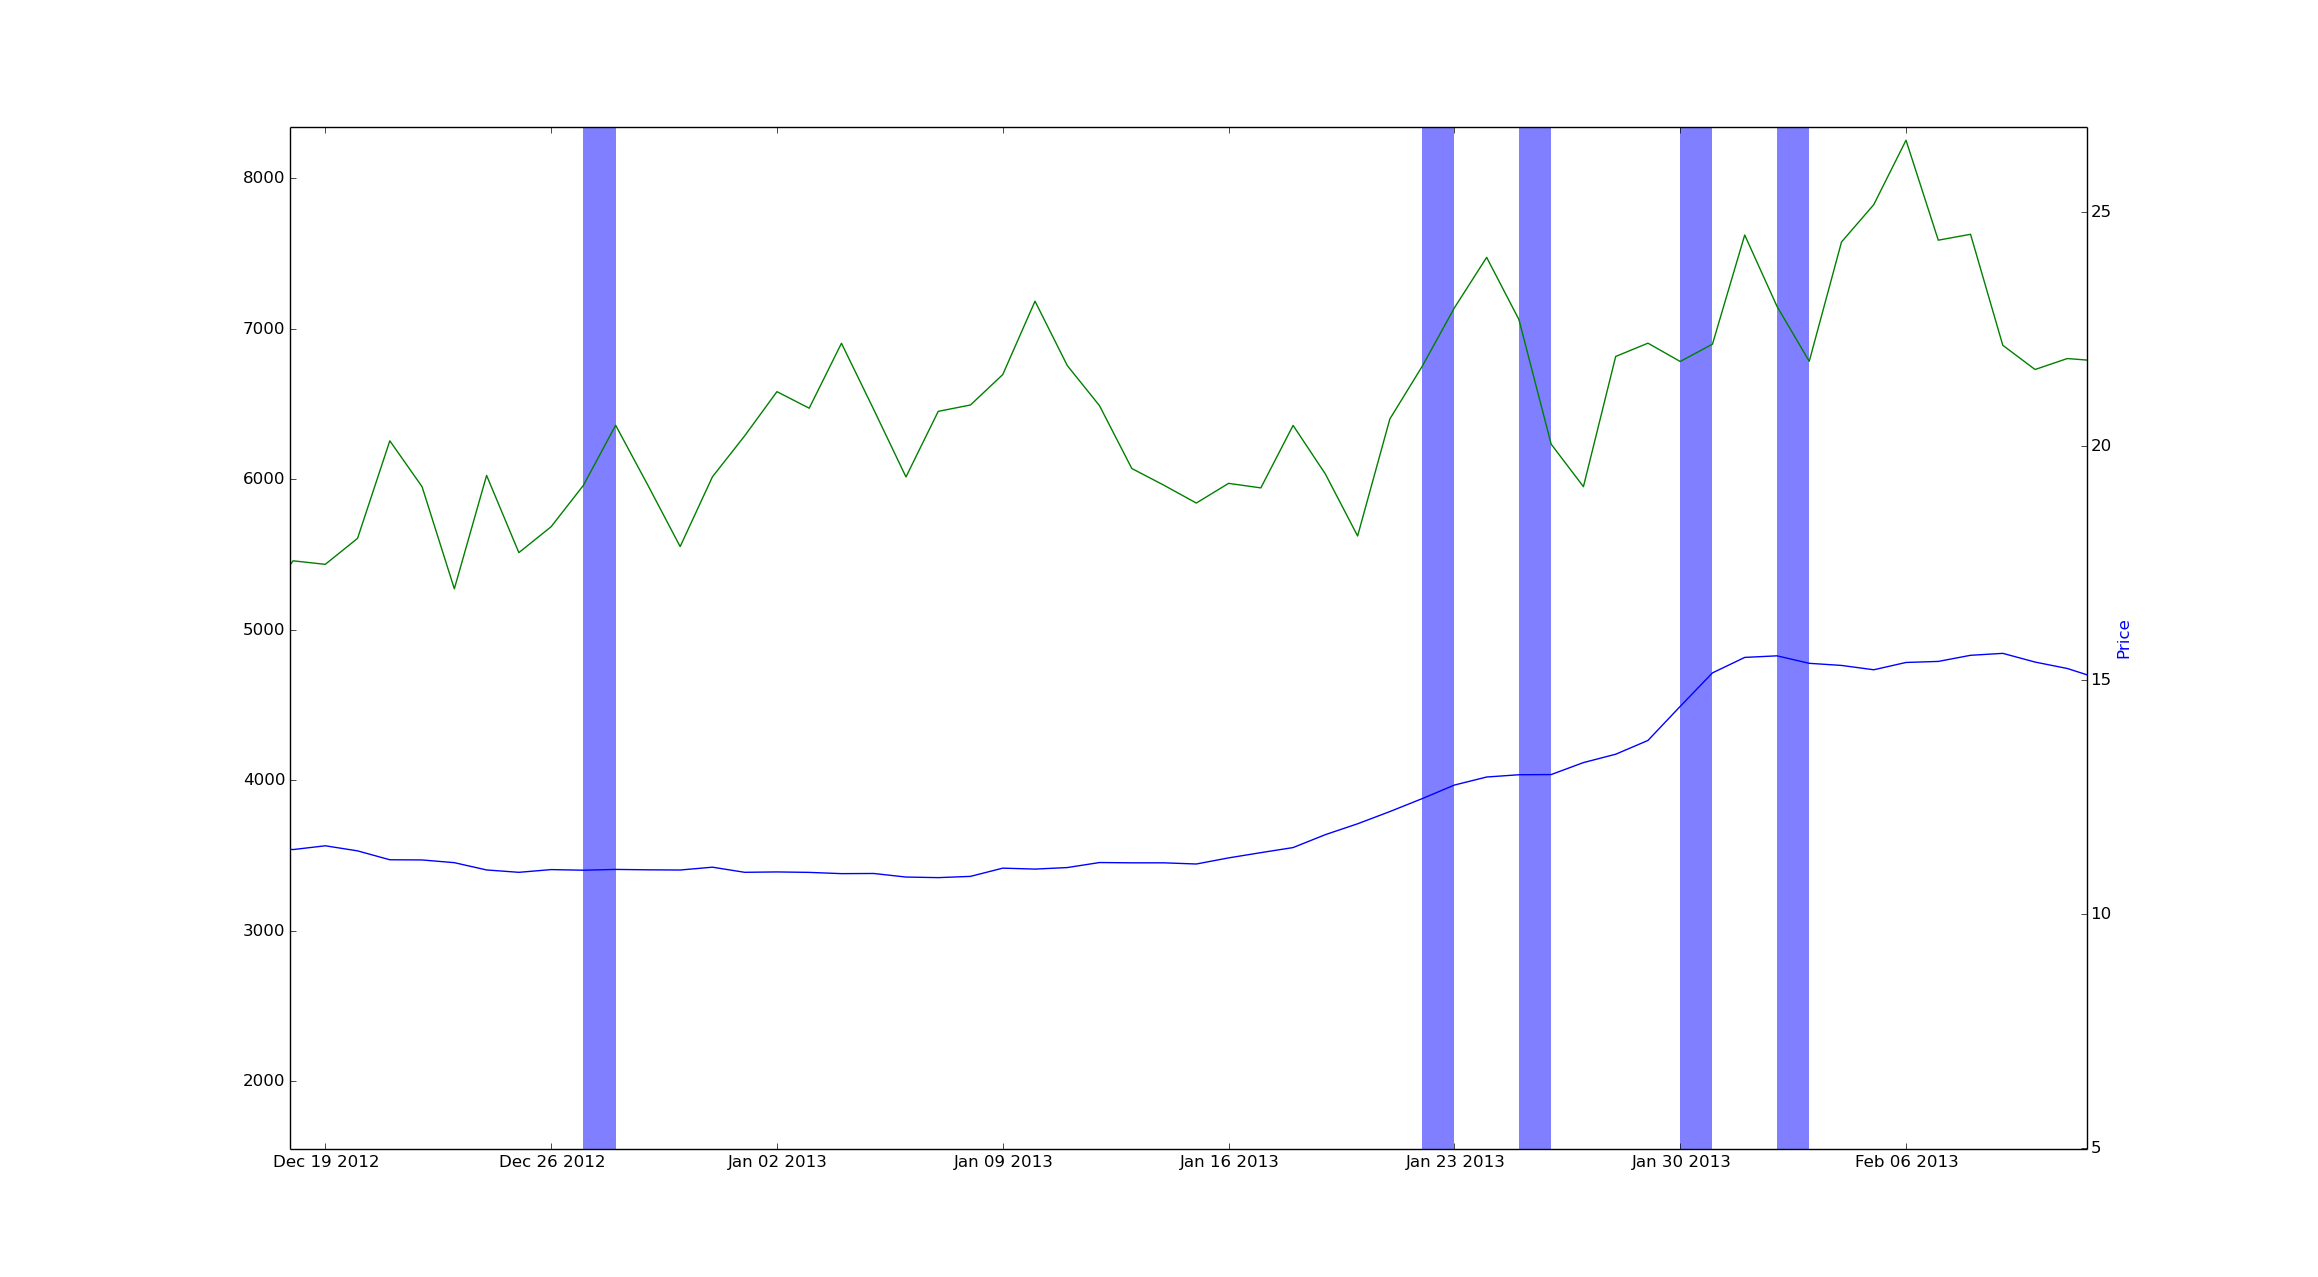
\includegraphics[width=0.8\textwidth]{graphs/12143.png}
		    	\caption{Slope Based Anomaly Detection (Green line - Arrival Data of Onion, Blue Line - Wholesale Price)}
		    	\label{fig:12143}
			\end{figure}
			
			\item There exist some cases where due to low arrival, prices went high and when slowly arrival started entering into market, prices were going down slowly. This period of slow decrement of prices is not reported by this method but since prices were still high, this system could not report dates for news articles corresponding to this tenure. Such cases occurred in \textit{Analysis 2} for Dec 2010 and Jan 2011 (See Figure \ref{fig:12124})and in \textit{Analysis 4} for Nov 2013 (See Figure \ref{fig:12144}). Also, note that these articles were mainly on Pakistan banned exports and article on inflation stating that inflation rate went high and onion prices are playing an important role in this.
			
			\begin{figure}[H]
		    	\centering
  		    	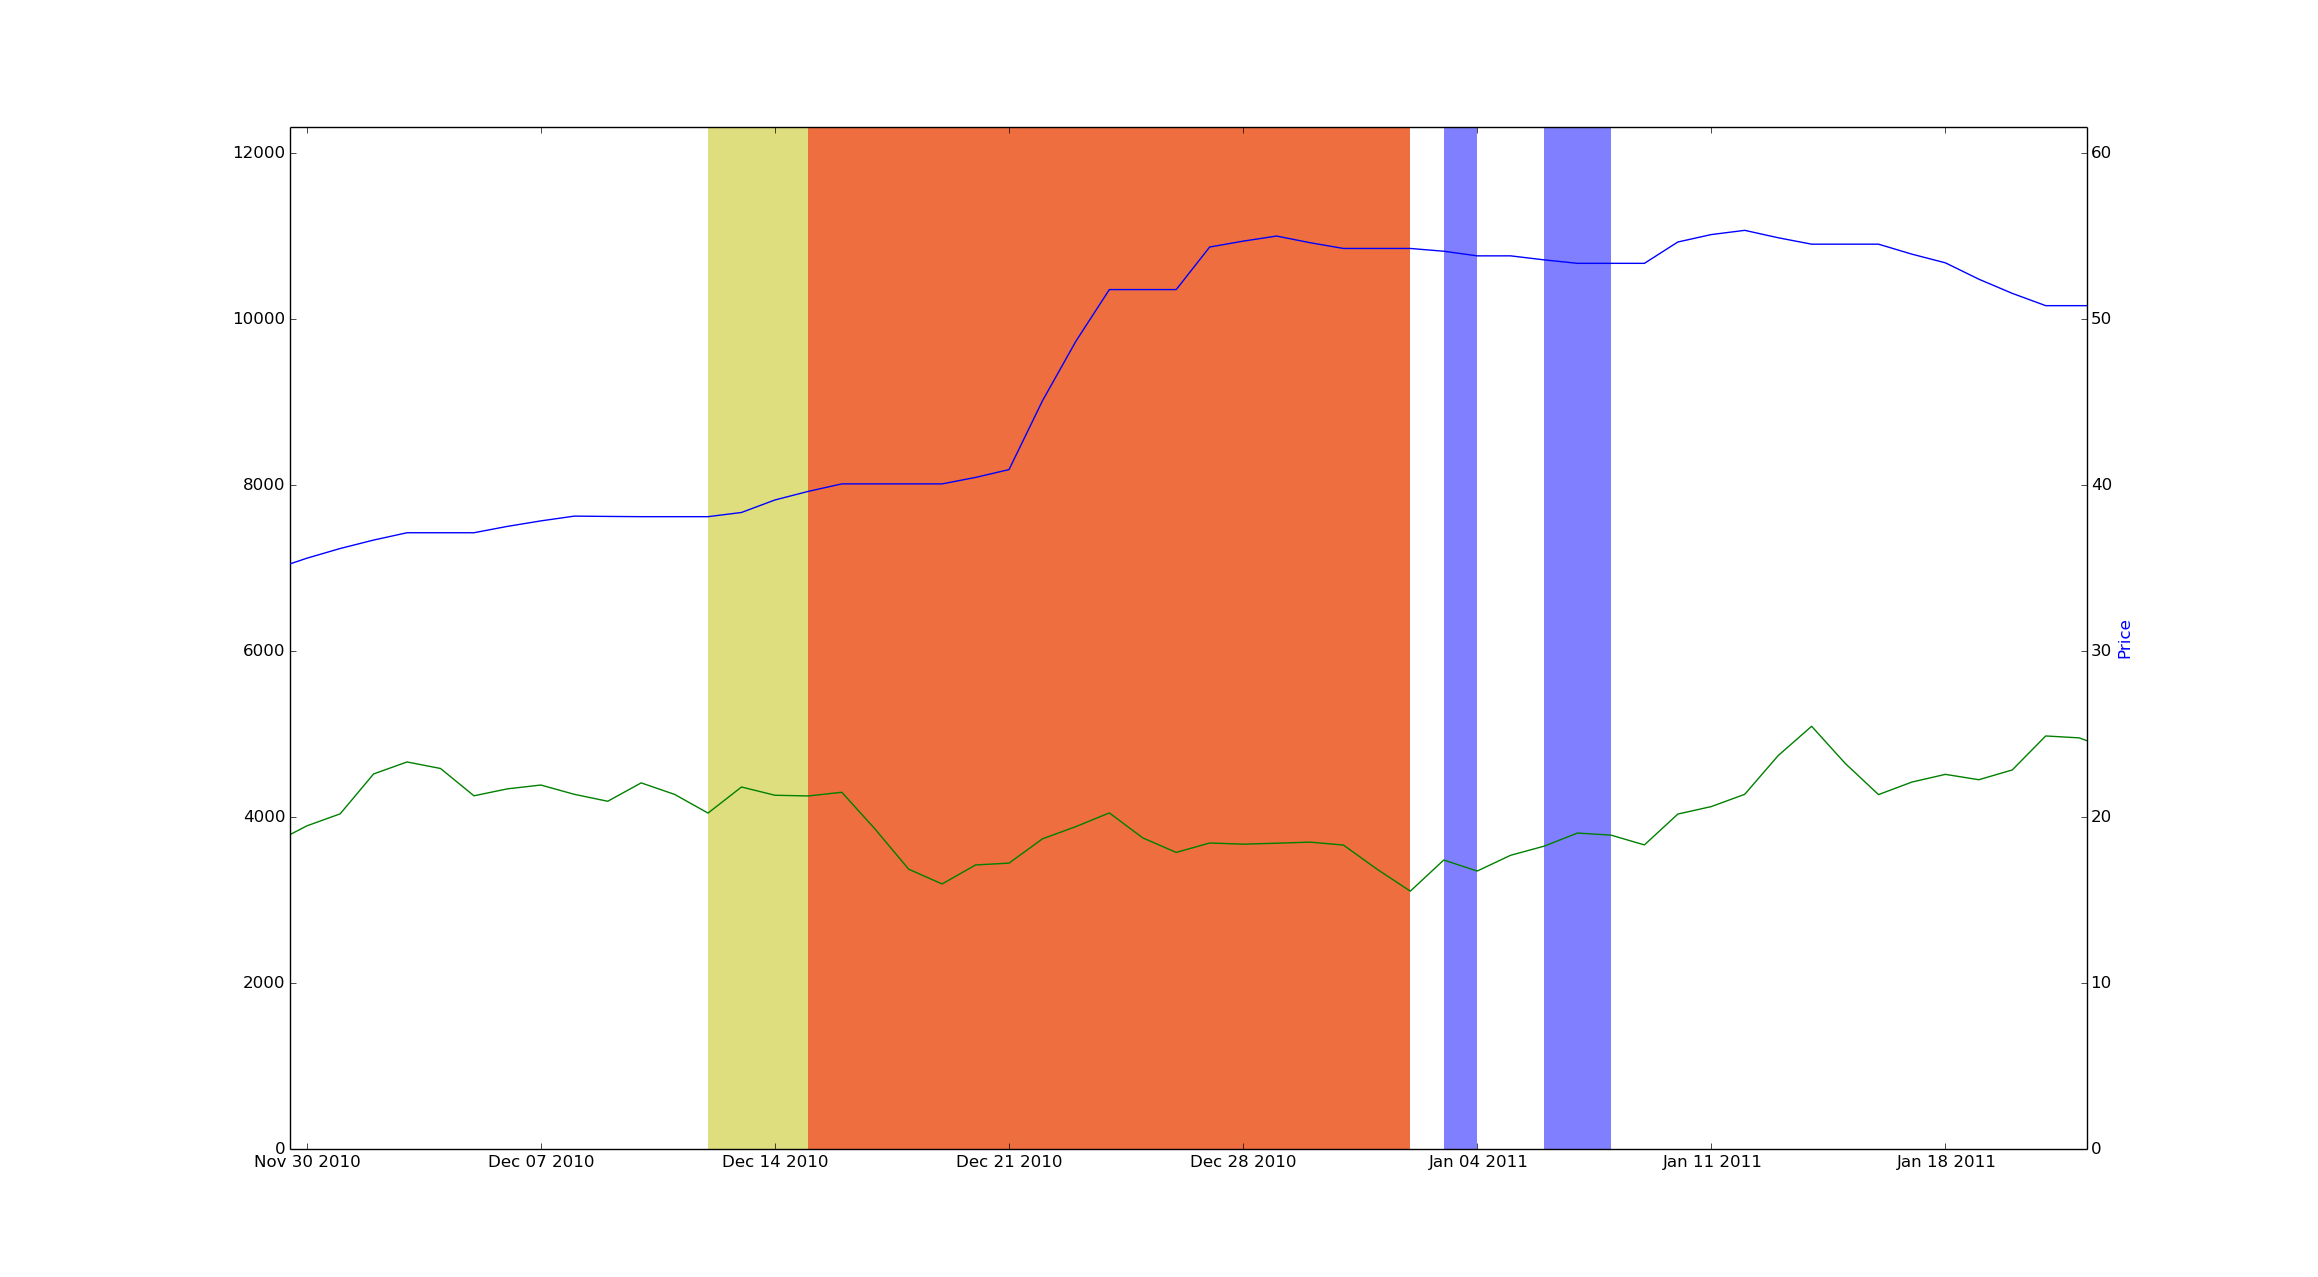
\includegraphics[width=0.8\textwidth]{graphs/12124.png}
		    	\caption{Slope Based Anomaly Detection (Green line - Arrival Data of Onion, Blue Line - Retail Price)}
		    	\label{fig:12124}
			\end{figure}
			
			\begin{figure}[H]
		    	\centering
  		    	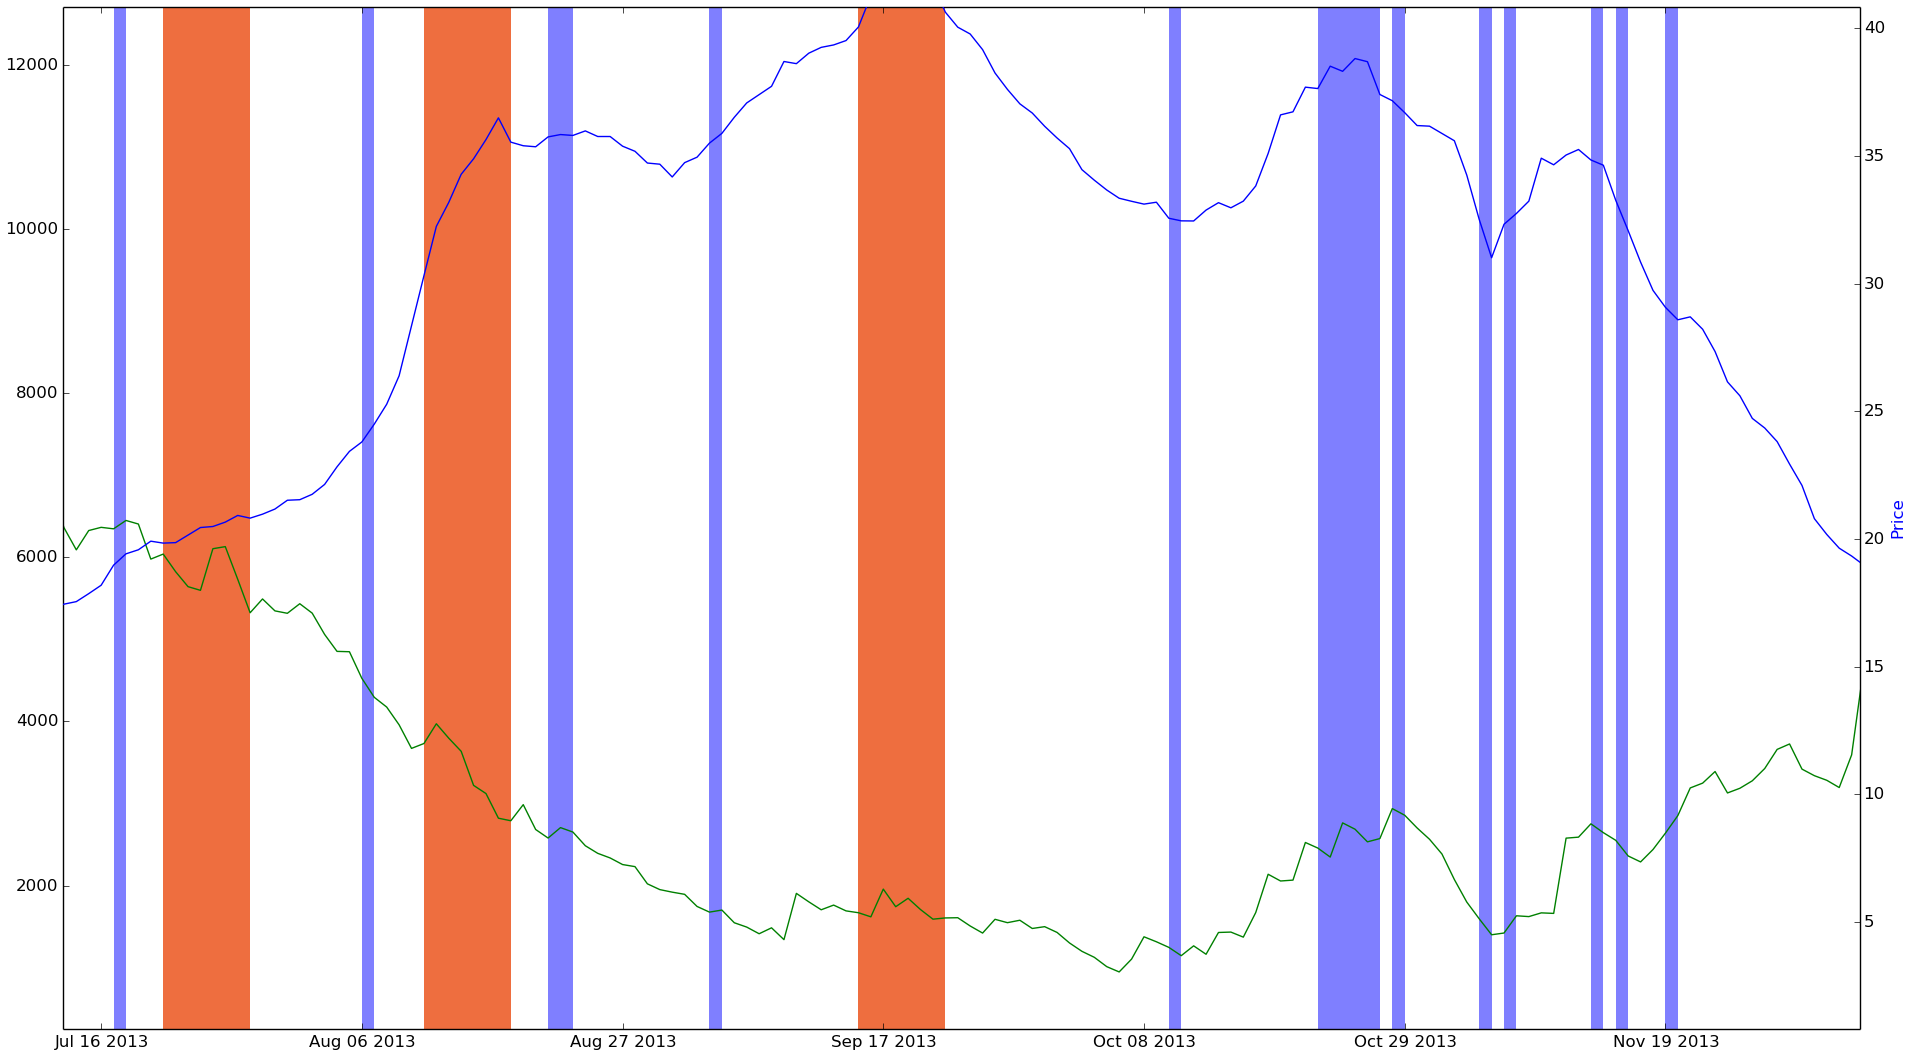
\includegraphics[width=0.8\textwidth]{graphs/12144.png}
		    	\caption{Slope Based Anomaly Detection (Green line - Arrival Data of Onion, Blue Line - Wholesale Price)}
		    	\label{fig:12144}
			\end{figure}
			
			\item In some of the cases where arrival fell drastically and due to that retail price went high drastically. Since retail prices went high too much, it got reported in news articles but this was expected as arrival was less. But here both the changes were high, so ultimately slope value was not so high and was not reported by system. Such cases in \textit{Analysis 2} exist for Aug Sept 2013  (See Figure \ref{fig:12125}).
			
			\begin{figure}[H]
		    	\centering
  		    	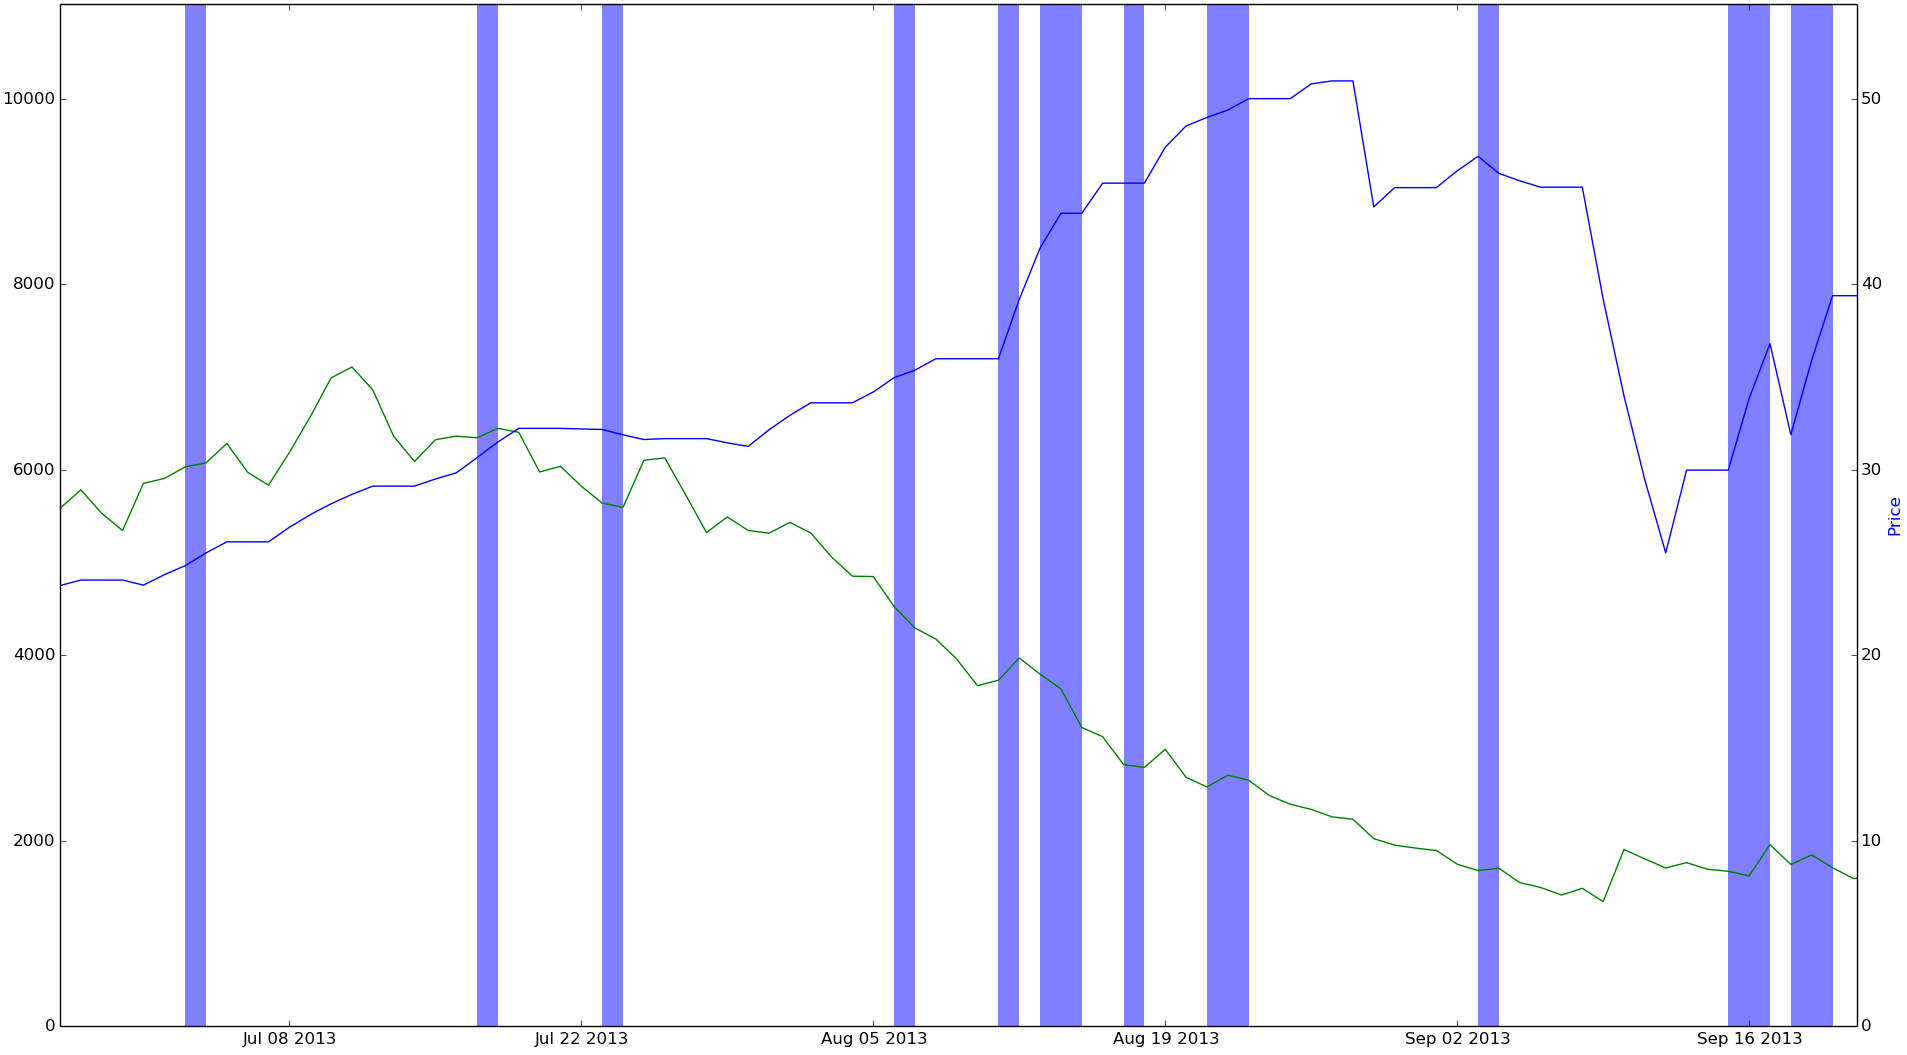
\includegraphics[width=0.8\textwidth]{graphs/12125.png}
		    	\caption{Slope Based Anomaly Detection (Green line - Arrival Data of Onion, Blue Line - Retail Price)}
		    	\label{fig:12125}
			\end{figure}
			
			\item Another limitation of this method is when retail price remained constant and there was change in arrival. As retail price was constant, slope value became zero and method did not report them and due to that few news articles could not be matched by dates reported by this method for example in \textit{Analysis 2}, this thing occurred for June July 2015  (See Figure \ref{fig:12126}).
			
			\begin{figure}[H]
		    	\centering
  		    	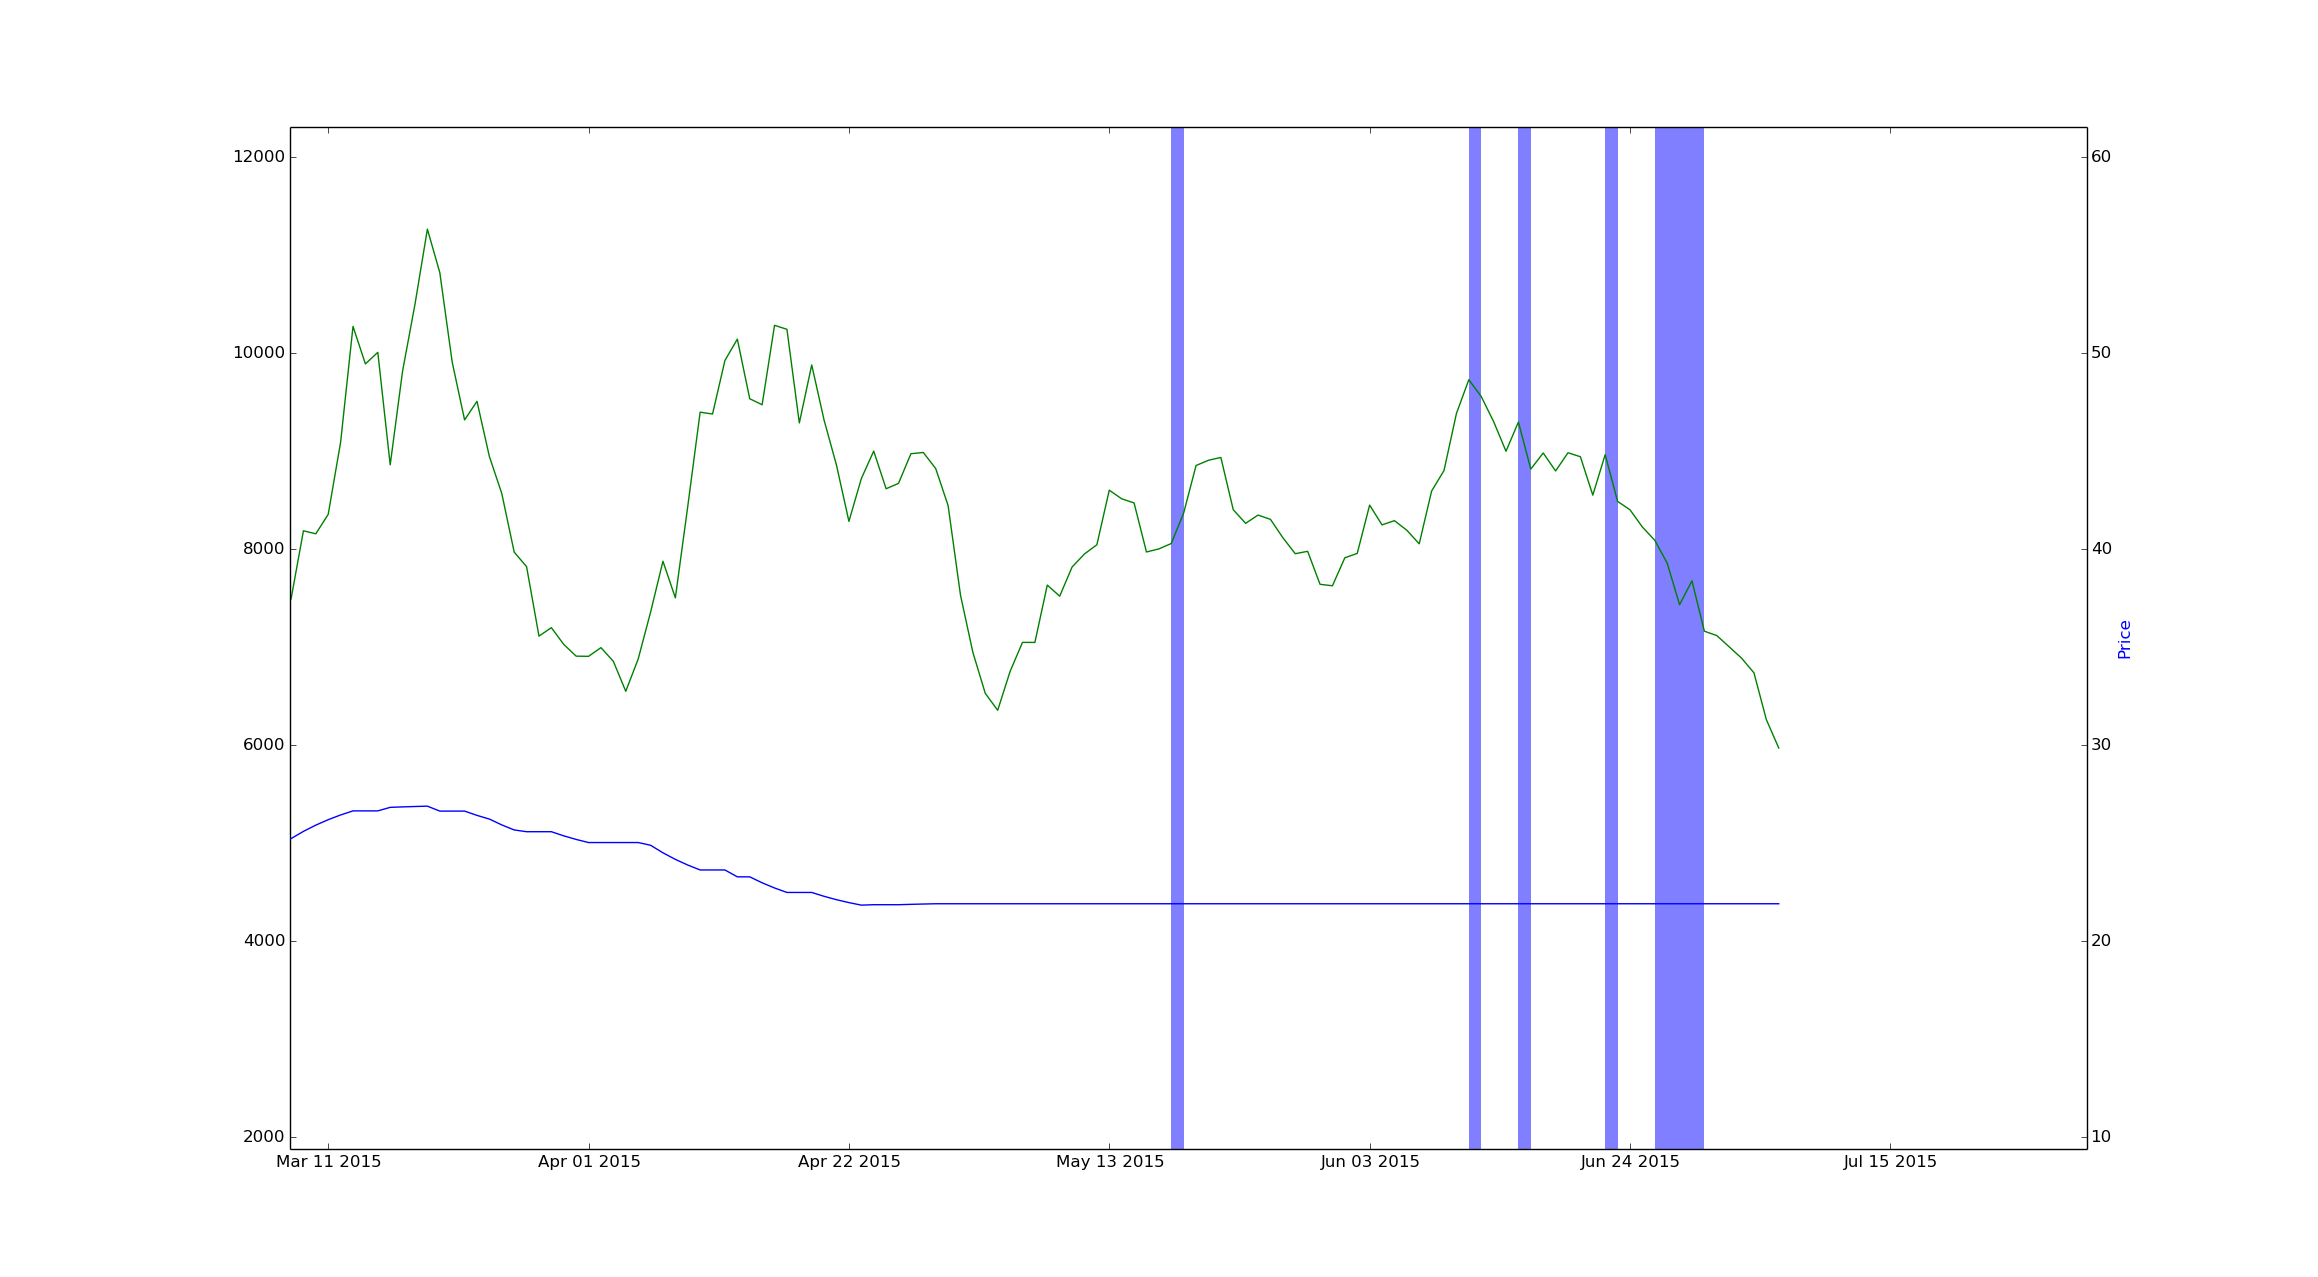
\includegraphics[width=0.8\textwidth]{graphs/12126.png}
		    	\caption{Slope Based Anomaly Detection (Green line - Arrival Data of Onion, Blue Line - Retail Price)}
		    	\label{fig:12126}
			\end{figure}
			
		\end{itemize}


	Also, note one thing that this method reports anomaly as whole window of few days (here 7 days). So because of that too, method tends to report more anomaly dates.


\subsection{Linear Regression}

		The main functionality of this method is to find what should be ideal value of the dependent variable given value of independent variable. This method first finds out linear relationship between 2 variables, whose time series is given as input and one of them is dependent on another. After finding out this equation, we see for a given value of independent variable what should be ideal value of dependent variable and note down the relative difference. If this difference is large, then it is reported as anomaly.\\
		\\
		We have four types of analysis which are as follows:
		\begin{enumerate}
			\item \textbf{Retail Price vs Average of Retail Price}: Here, we first take average of retail price at all centres as independent variable and retail price as dependent variable.			
			\item \textbf{Retail Price vs Arrival of Onion}: Here, we take retail price as dependent variable and arrival of onion as independent variable.
			\item \textbf{Retail Price vs Wholesale Price}: Here, we take retail price as dependent variable and Wholesale Price as independent variable.
			\item \textbf{Wholesale Price vs Arrival of Onion}: Here, we take Wholesale price as dependent variable and arrival of onion as independent variable.
		\end{enumerate}
		
		So, in each of the case, we try to find relative difference between ideal value and its real value, and if it is huge (crosses threshold) then it is reported as anomaly. Now, note that in analysis 1 and 3 stated above, both the time series are directly proportional to each other and in the analysis 2 and 4 both the time series are inversely proportional to each other. So, limitations faced by this method for analysis 1 and 3 will be similar and for analysis 2 and 4 will be similar. While describing this method, each analysis will be referenced by its corresponding number.\\
		\\
		First we will start with analysis 1 and 3. Following are the few observations we made:
		
		\begin{itemize}
			\item This method will report any tenure as anomaly when there is large gap i.e. more than expected between retail price of a center and average retail price (for \textit{Analysis 1}) or wholesale price (for \textit{Analysis 3}).
			
			
			
			Following tenures are some cases reported by this method:
			\begin{itemize}
				\item \textit{Analysis 1}: Dec 2010, Near to Jan 2011, May June July 2011, Jan May June 2012, June 2013 (See Figure \ref{fig:12211})
				\item \textit{Analysis 3}: Feb Mar 2011, Jan 2012, June 2012, Jan Feb 2014, Apr 2015 (See Figure \ref{fig:12231})
			\end{itemize}
			\begin{figure}[H]
		    	\centering
  		    	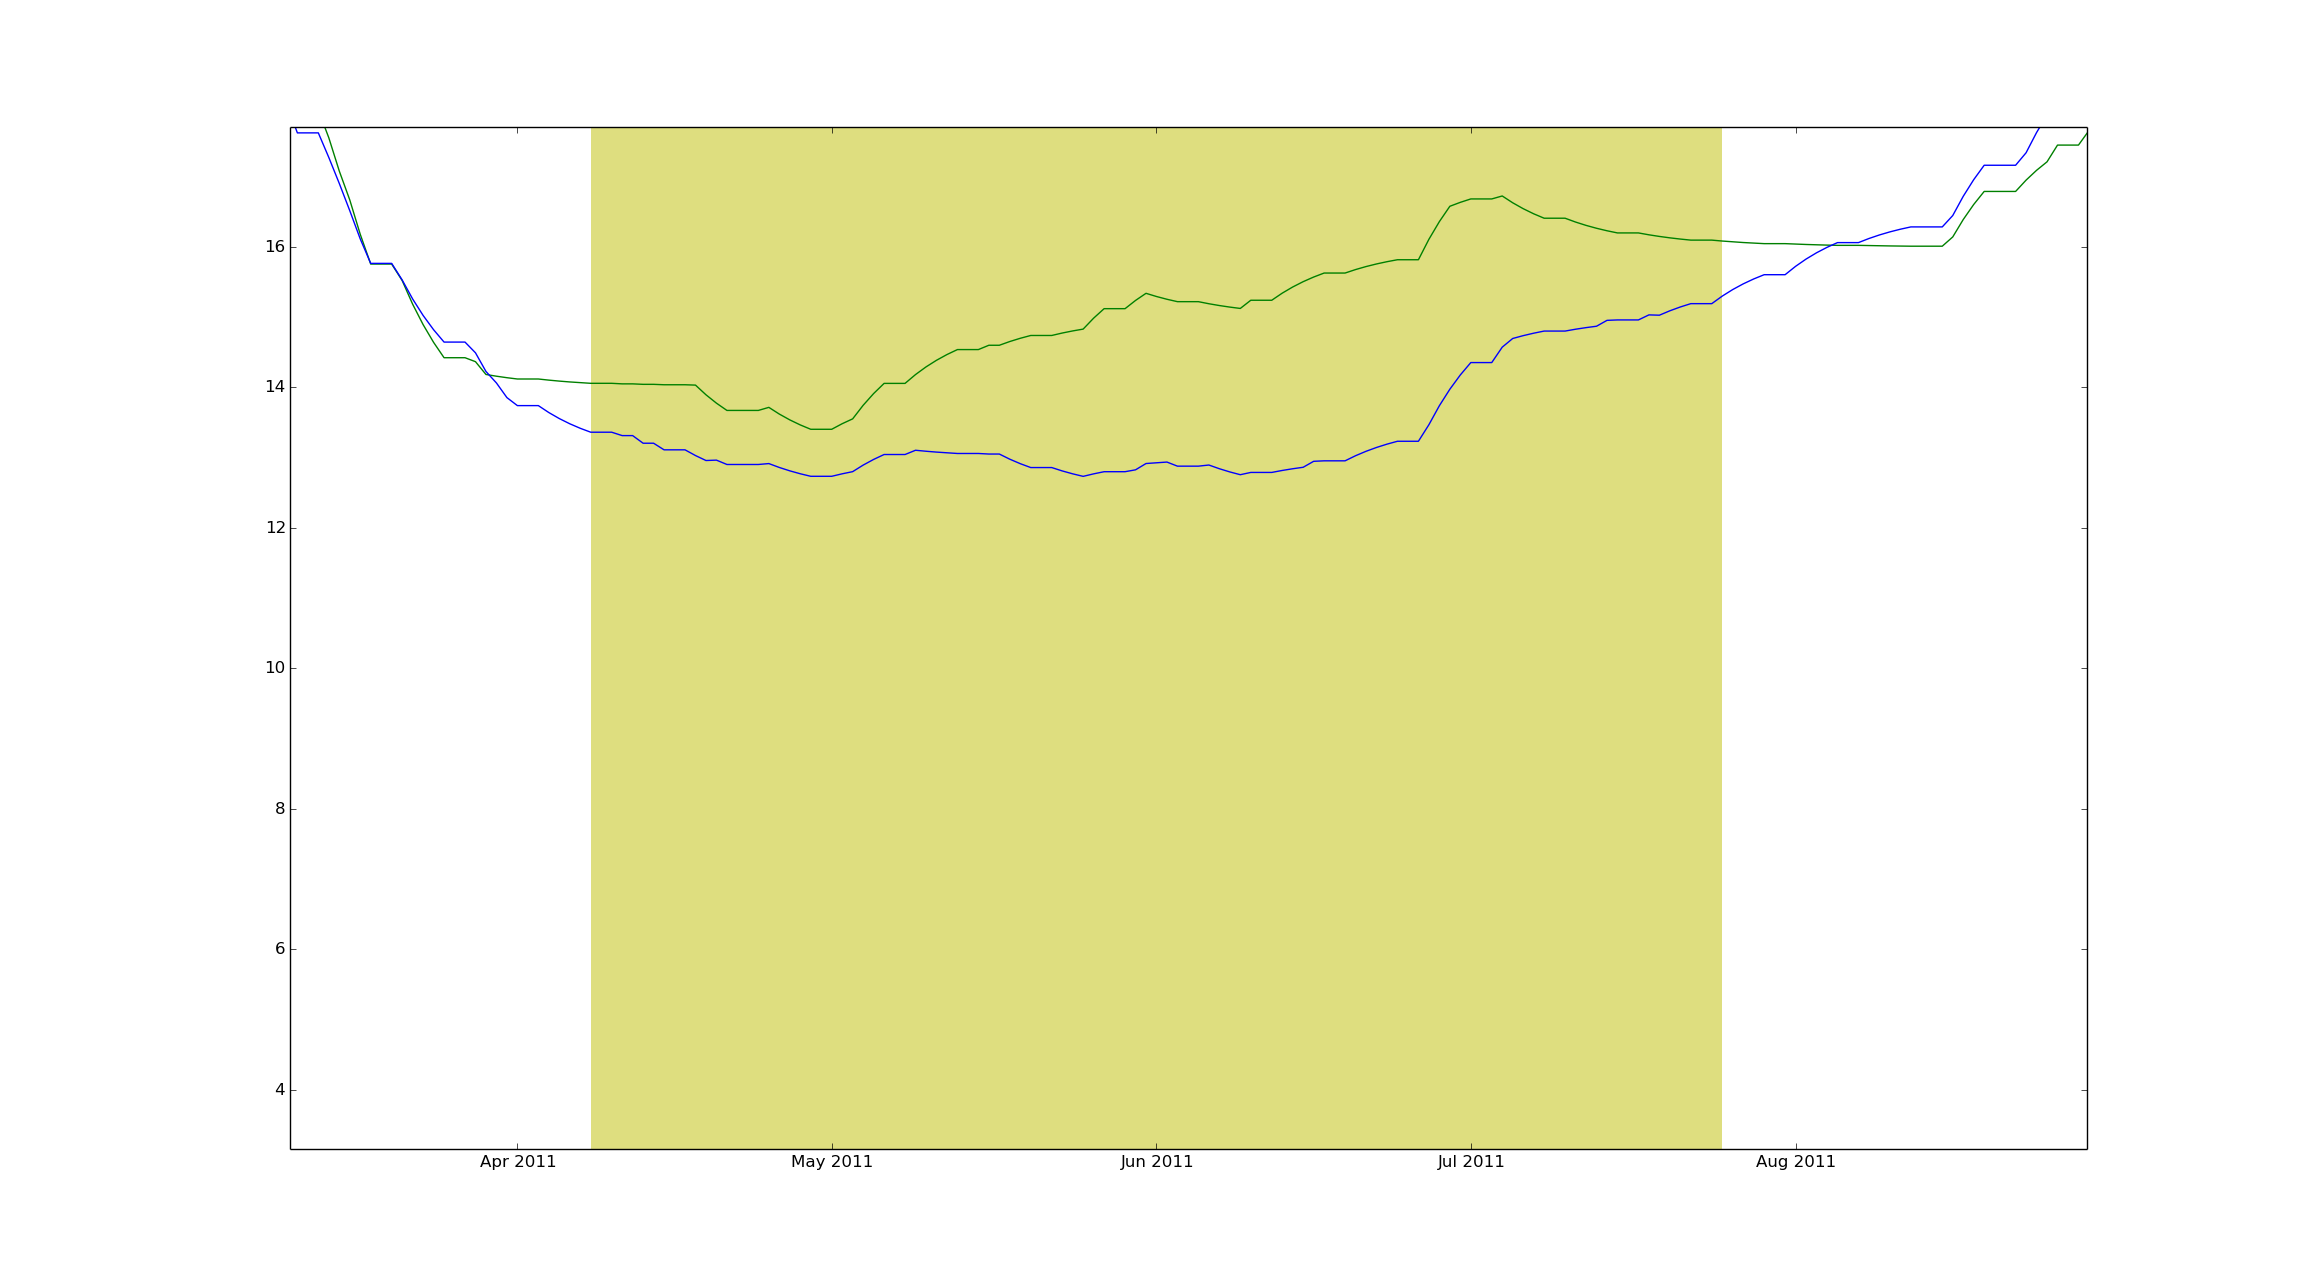
\includegraphics[width=0.8\textwidth]{graphs/12211.png}
		    	\caption{Linear Regression (Green line - Centre Retail Price, Blue Line - Average Retail Price)}
		    	\label{fig:12211}
			\end{figure}
			
			\begin{figure}[H]
		    	\centering
  		    	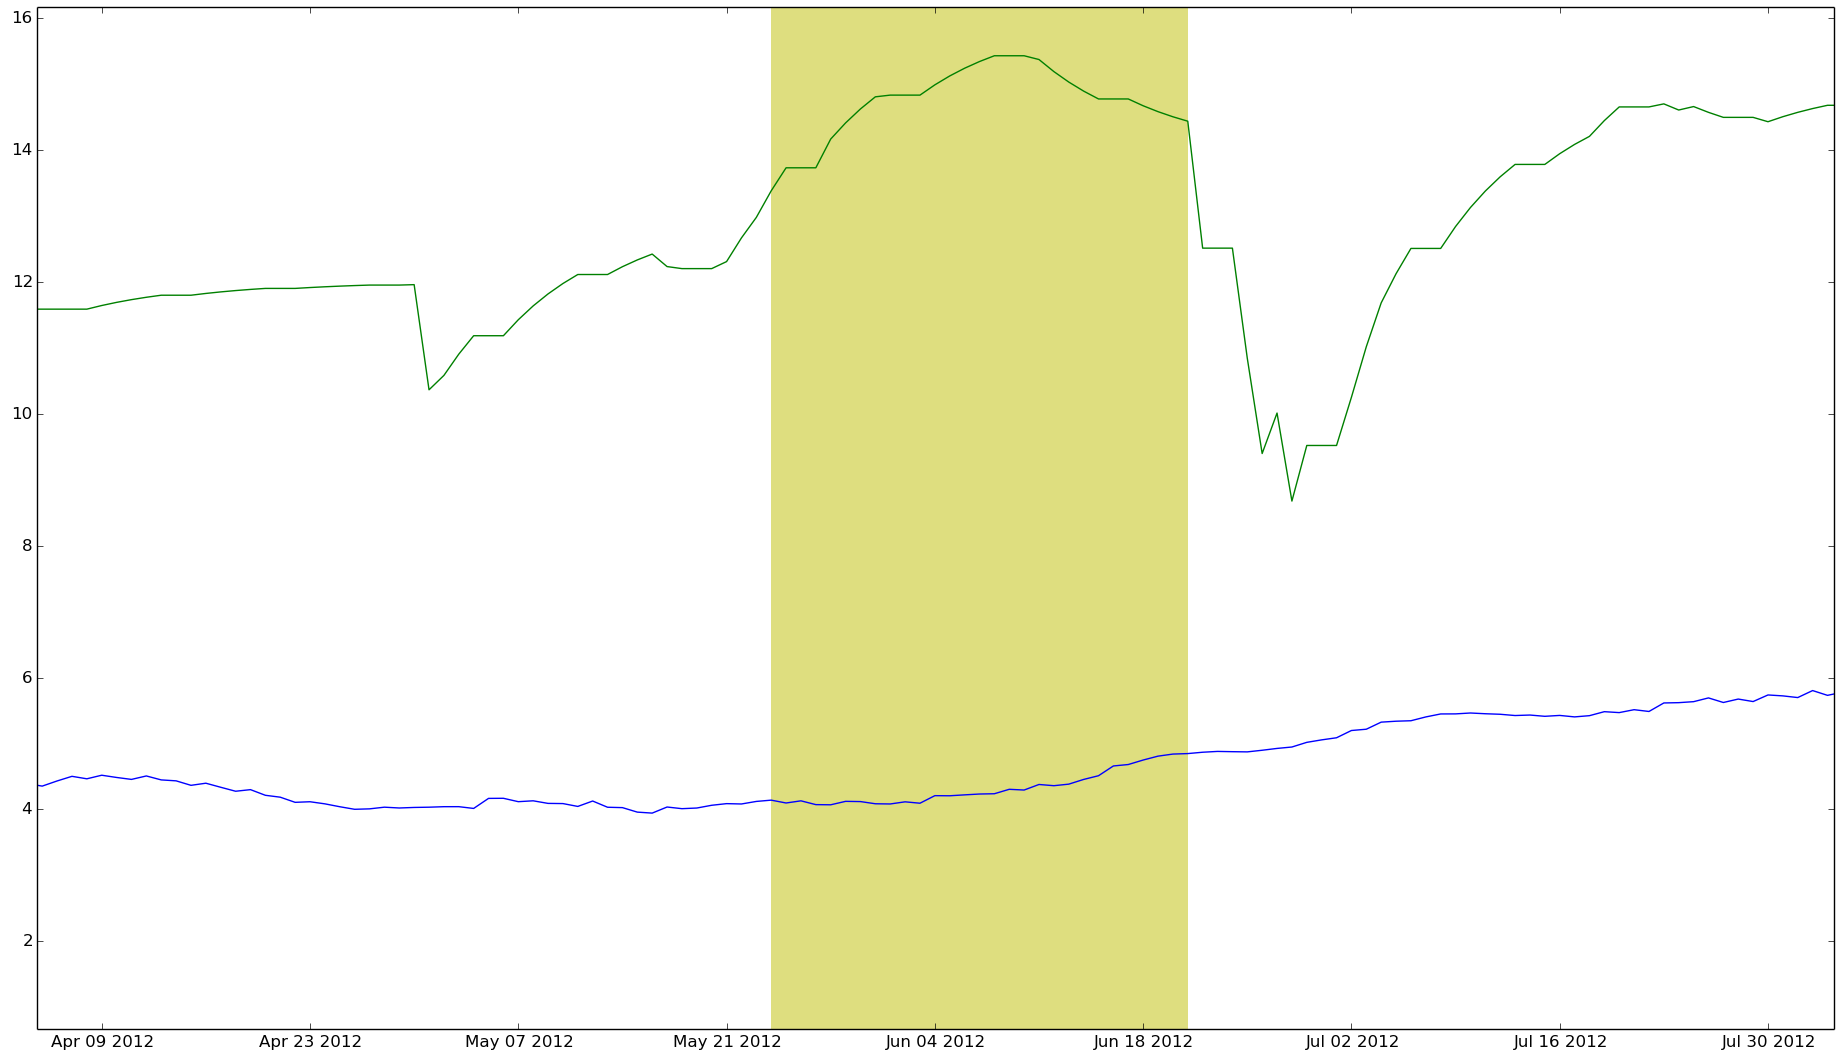
\includegraphics[width=0.8\textwidth]{graphs/12231.png}
		    	\caption{Linear Regression (Green line - Retail Price, Blue Line - Wholesale Price)}
		    	\label{fig:12231}
			\end{figure}
			
			\item One limitation of this method is that, if both the series have high values for some time period and difference between them is not so huge then that will not be reported as anomaly.	\\
			\\
			Following tenures are some cases reported by this method:
			\begin{itemize}
				\item \textit{Analysis 1}: Jan 2011, Jan Feb Aug Sept Oct Nov 2013, July 2014, June July 2015 (See Figure \ref{fig:12212})
				\item \textit{Analysis 3}: Feb 2013, Aug Sept Oct Nov 2013, June July 2015 (See Figure \ref{fig:12232})
			\end{itemize}
			\begin{figure}[H]
		    	\centering
  		    	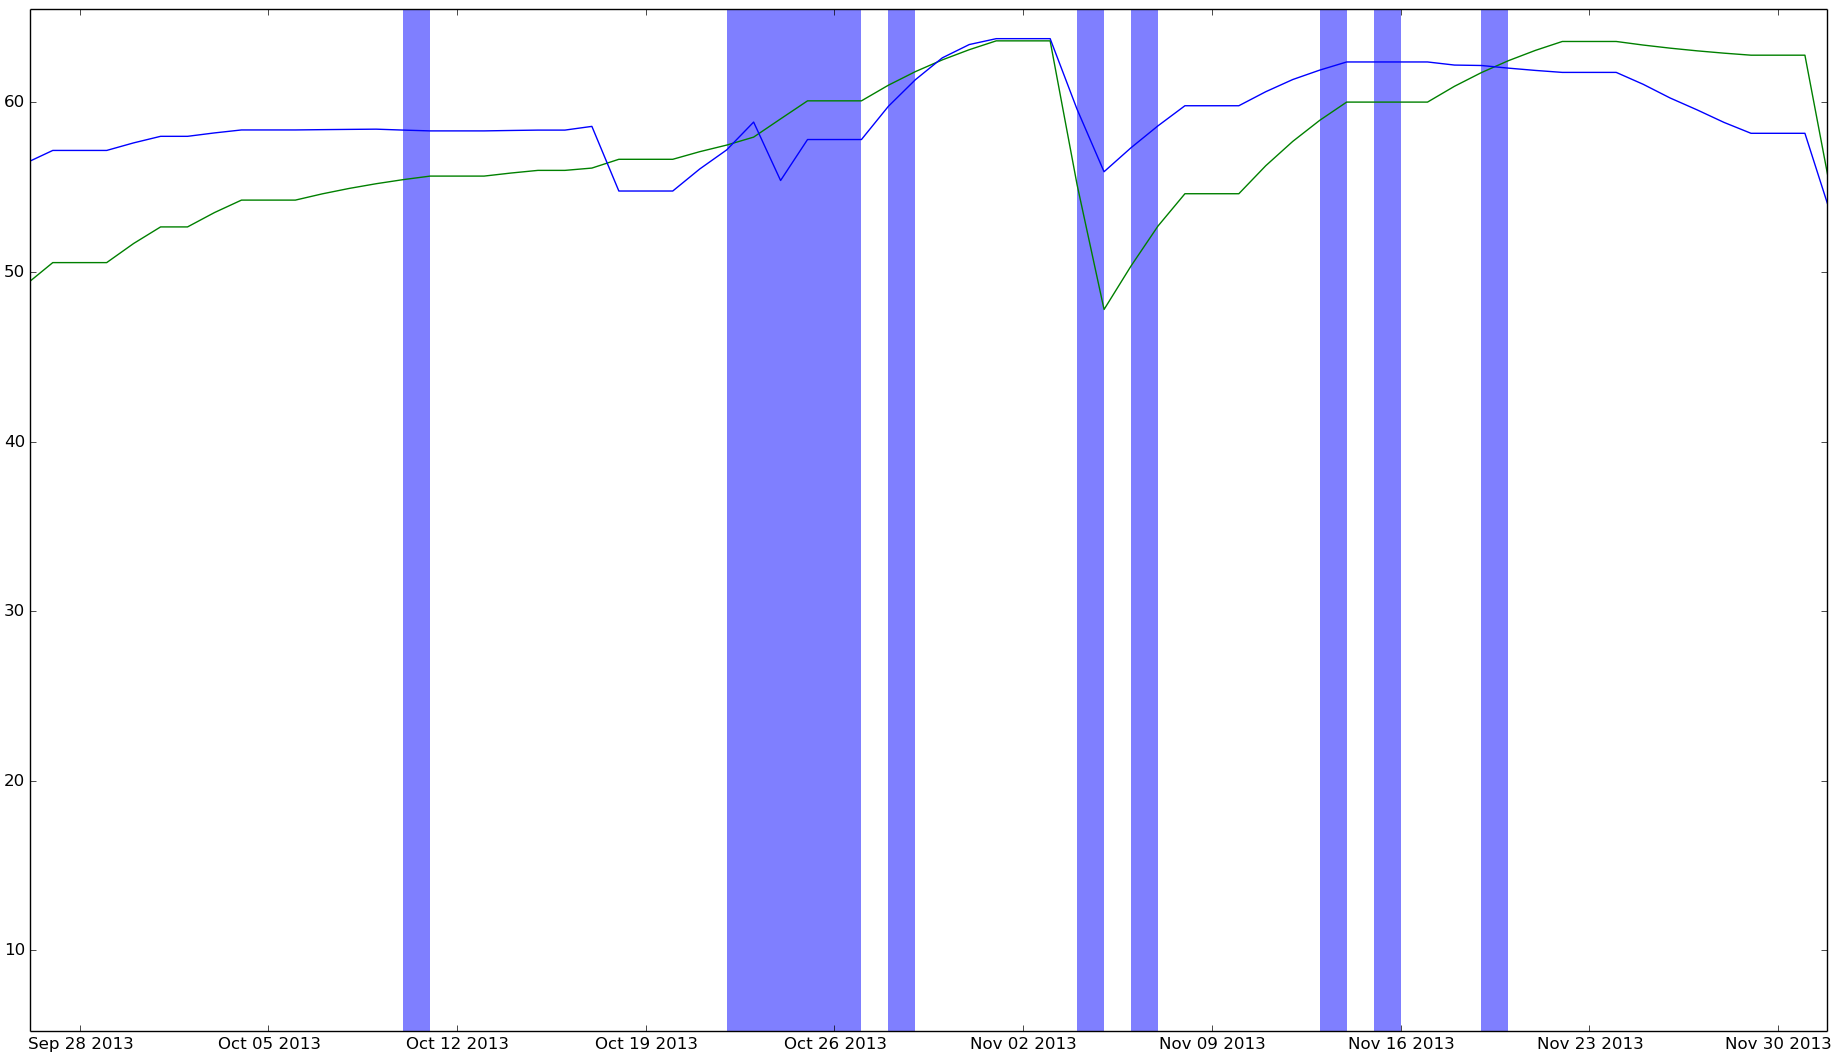
\includegraphics[width=0.8\textwidth]{graphs/12212.png}
		    	\caption{Linear Regression (Green line - Centre Retail Price, Blue Line - Average Retail Price)}
		    	\label{fig:12212}
			\end{figure}
			
			\begin{figure}[H]
		    	\centering
  		    	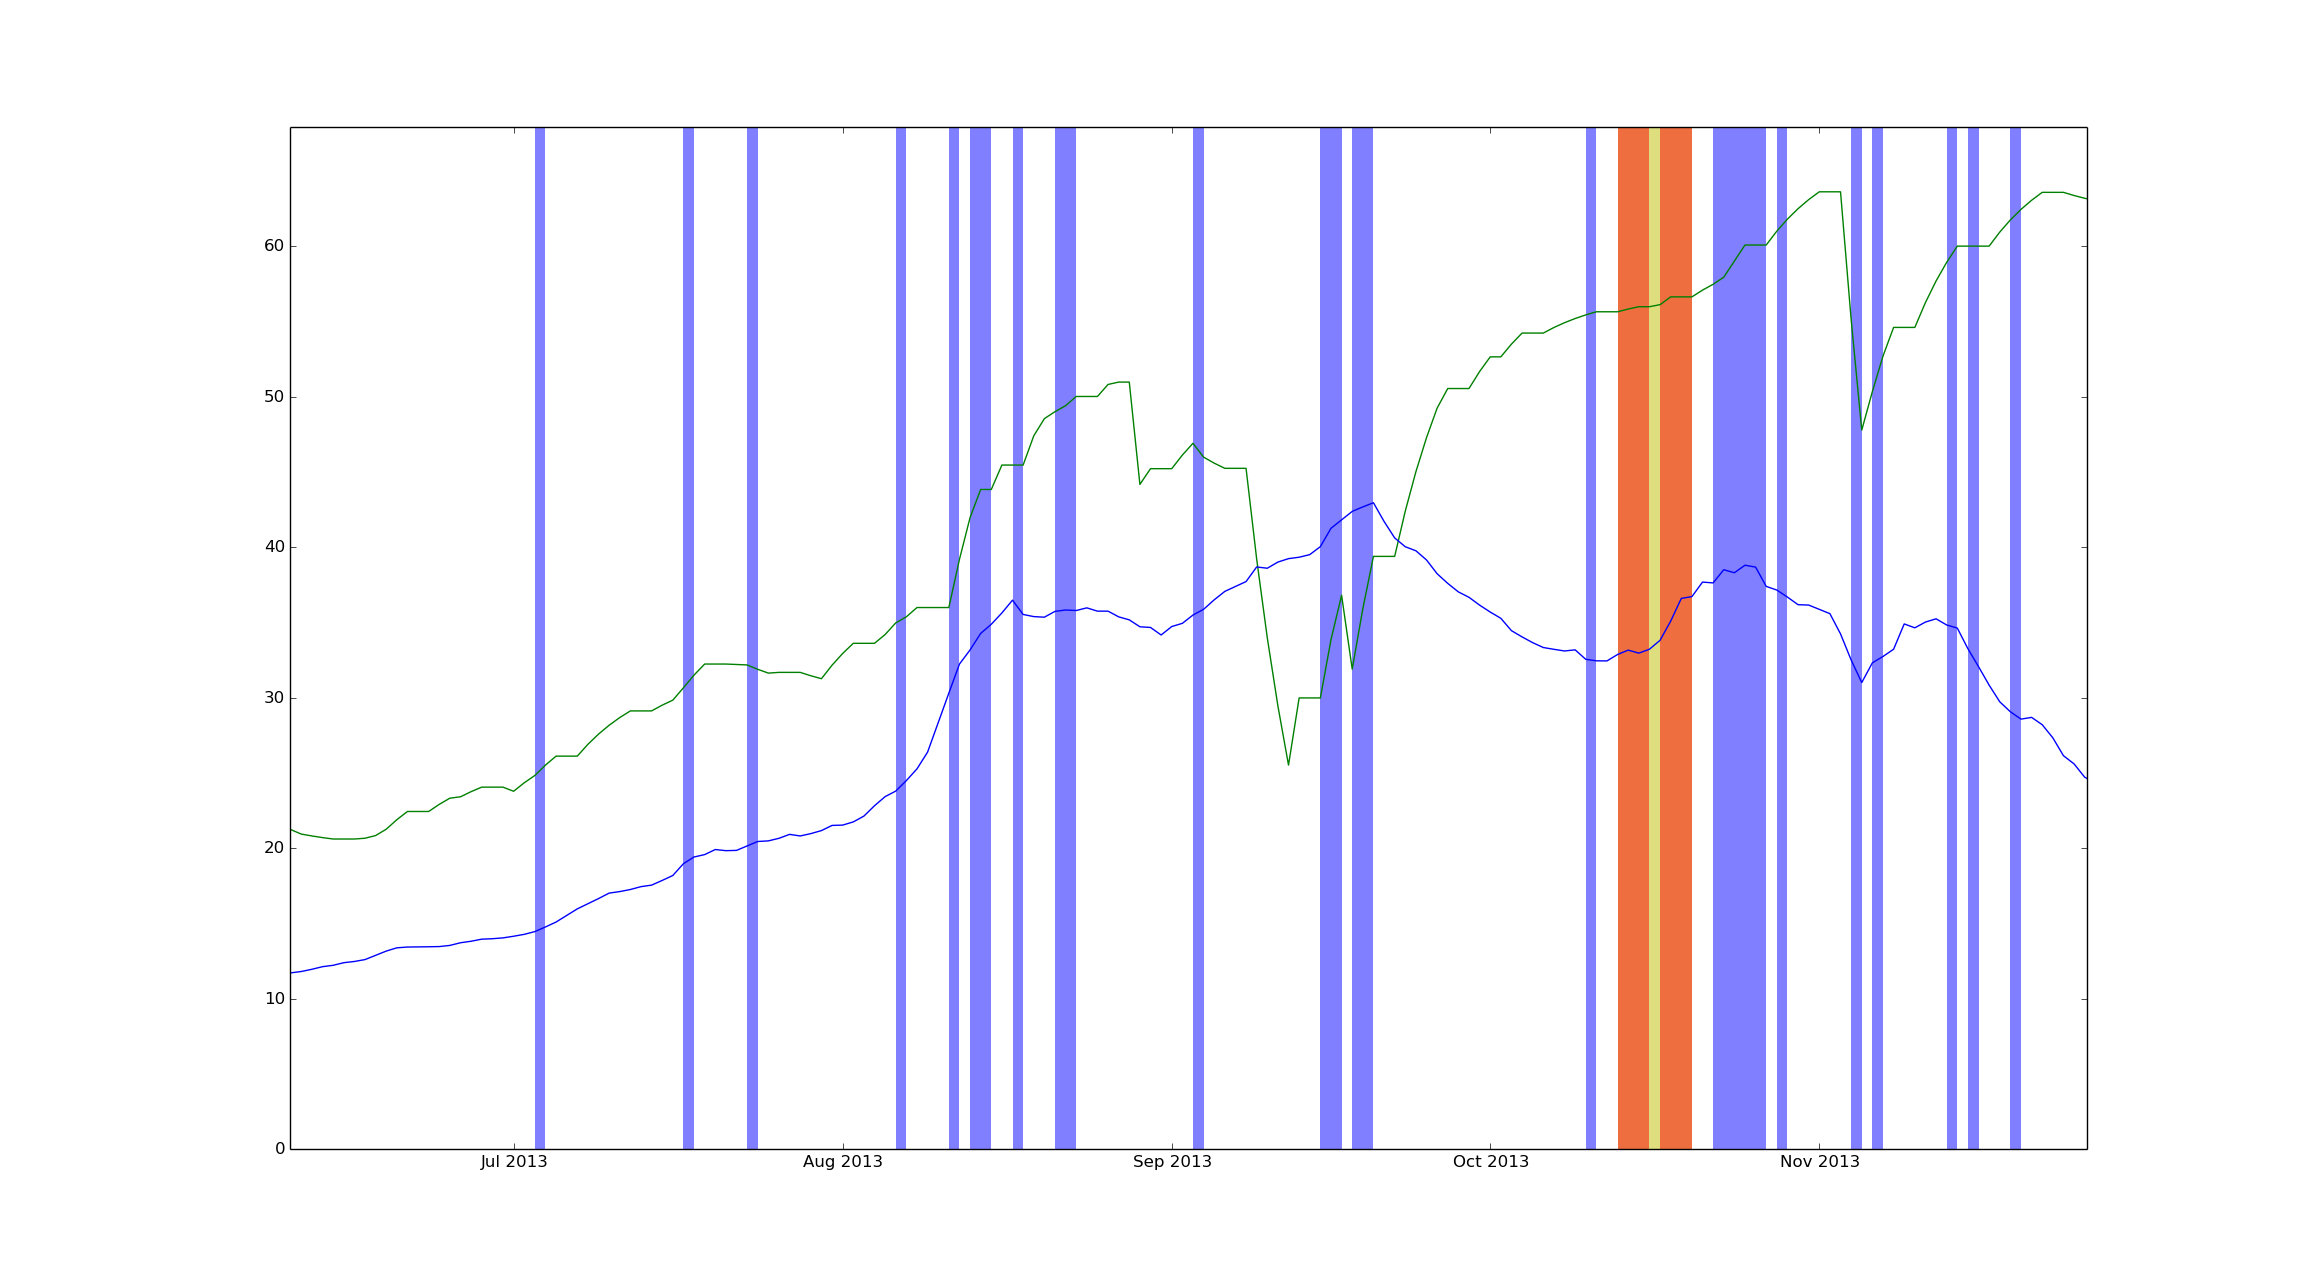
\includegraphics[width=0.8\textwidth]{graphs/12232.png}
		    	\caption{Linear Regression (Green line - Retail Price, Blue Line - Wholesale Price)}
		    	\label{fig:12232}
			\end{figure}
			
					
			
			\item  Note that in the tenure of Oct Nov 2013 (for \textit{Analysis 1}) prices are usually high and as the prices are high, tolerance level also increases little bit. So, even if for some difference it is reported as anomaly at lower price, it is not necessary that for the same difference, it will be reported as anomaly at higher prices. (See Figure \ref{fig:12212})		
			
		\end{itemize}
		
		
		Now we present few observation for Analysis 2 and 4.
		
		
		\begin{itemize}
			\item Here, in this method, it tries to predict what should be retail price or wholesale price based on the arrival of the product. So if the price is too high for the given arrival then it will be reported as anomaly.
			Following tenures are some cases reported by this method:
			\begin{itemize}
				\item \textit{Analysis 2}: Dec 2010, Jan Feb 2011, Aug Sept Oct Nov 2013, Oct Dec 2014 (See Figure \ref{fig:12221})
				\item \textit{Analysis 4}: Dec 2010, July Aug Sept Oct Nov Dec 2013, July 2014 (See Figure \ref{fig:12241})
			\end{itemize}
			\begin{figure}[H]
		    	\centering
  		    	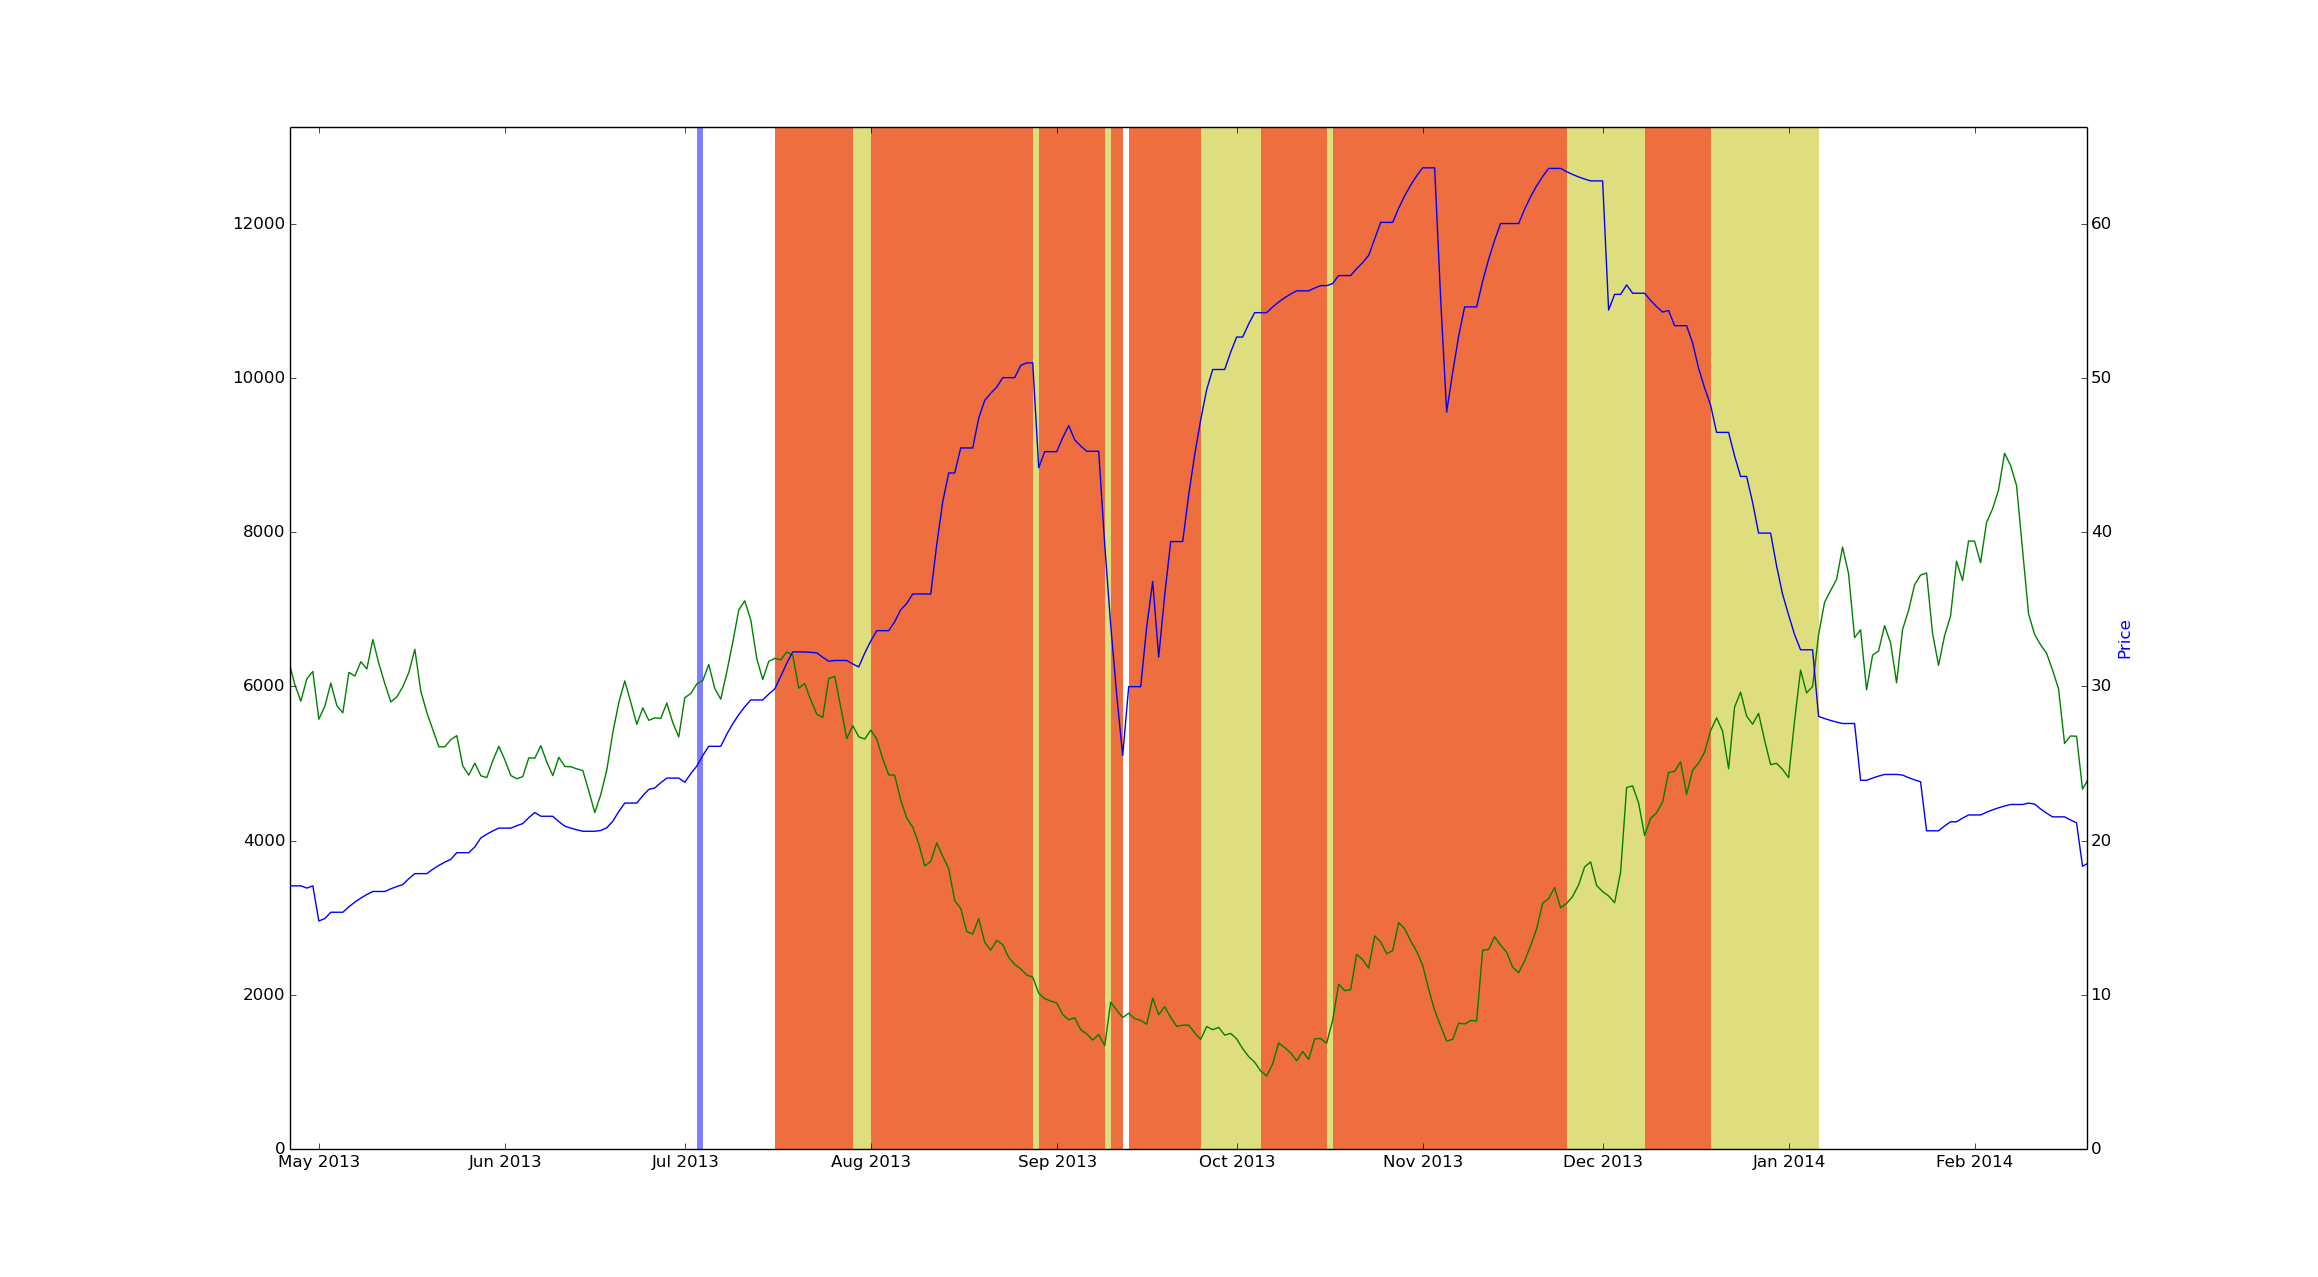
\includegraphics[width=0.8\textwidth]{graphs/12221.png}
		    	\caption{Linear Regression (Green line - Arrival Data of Onion, Blue Line - Retail Price)}
		    	\label{fig:12221}
			\end{figure}
			
			\begin{figure}[H]
		    	\centering
  		    	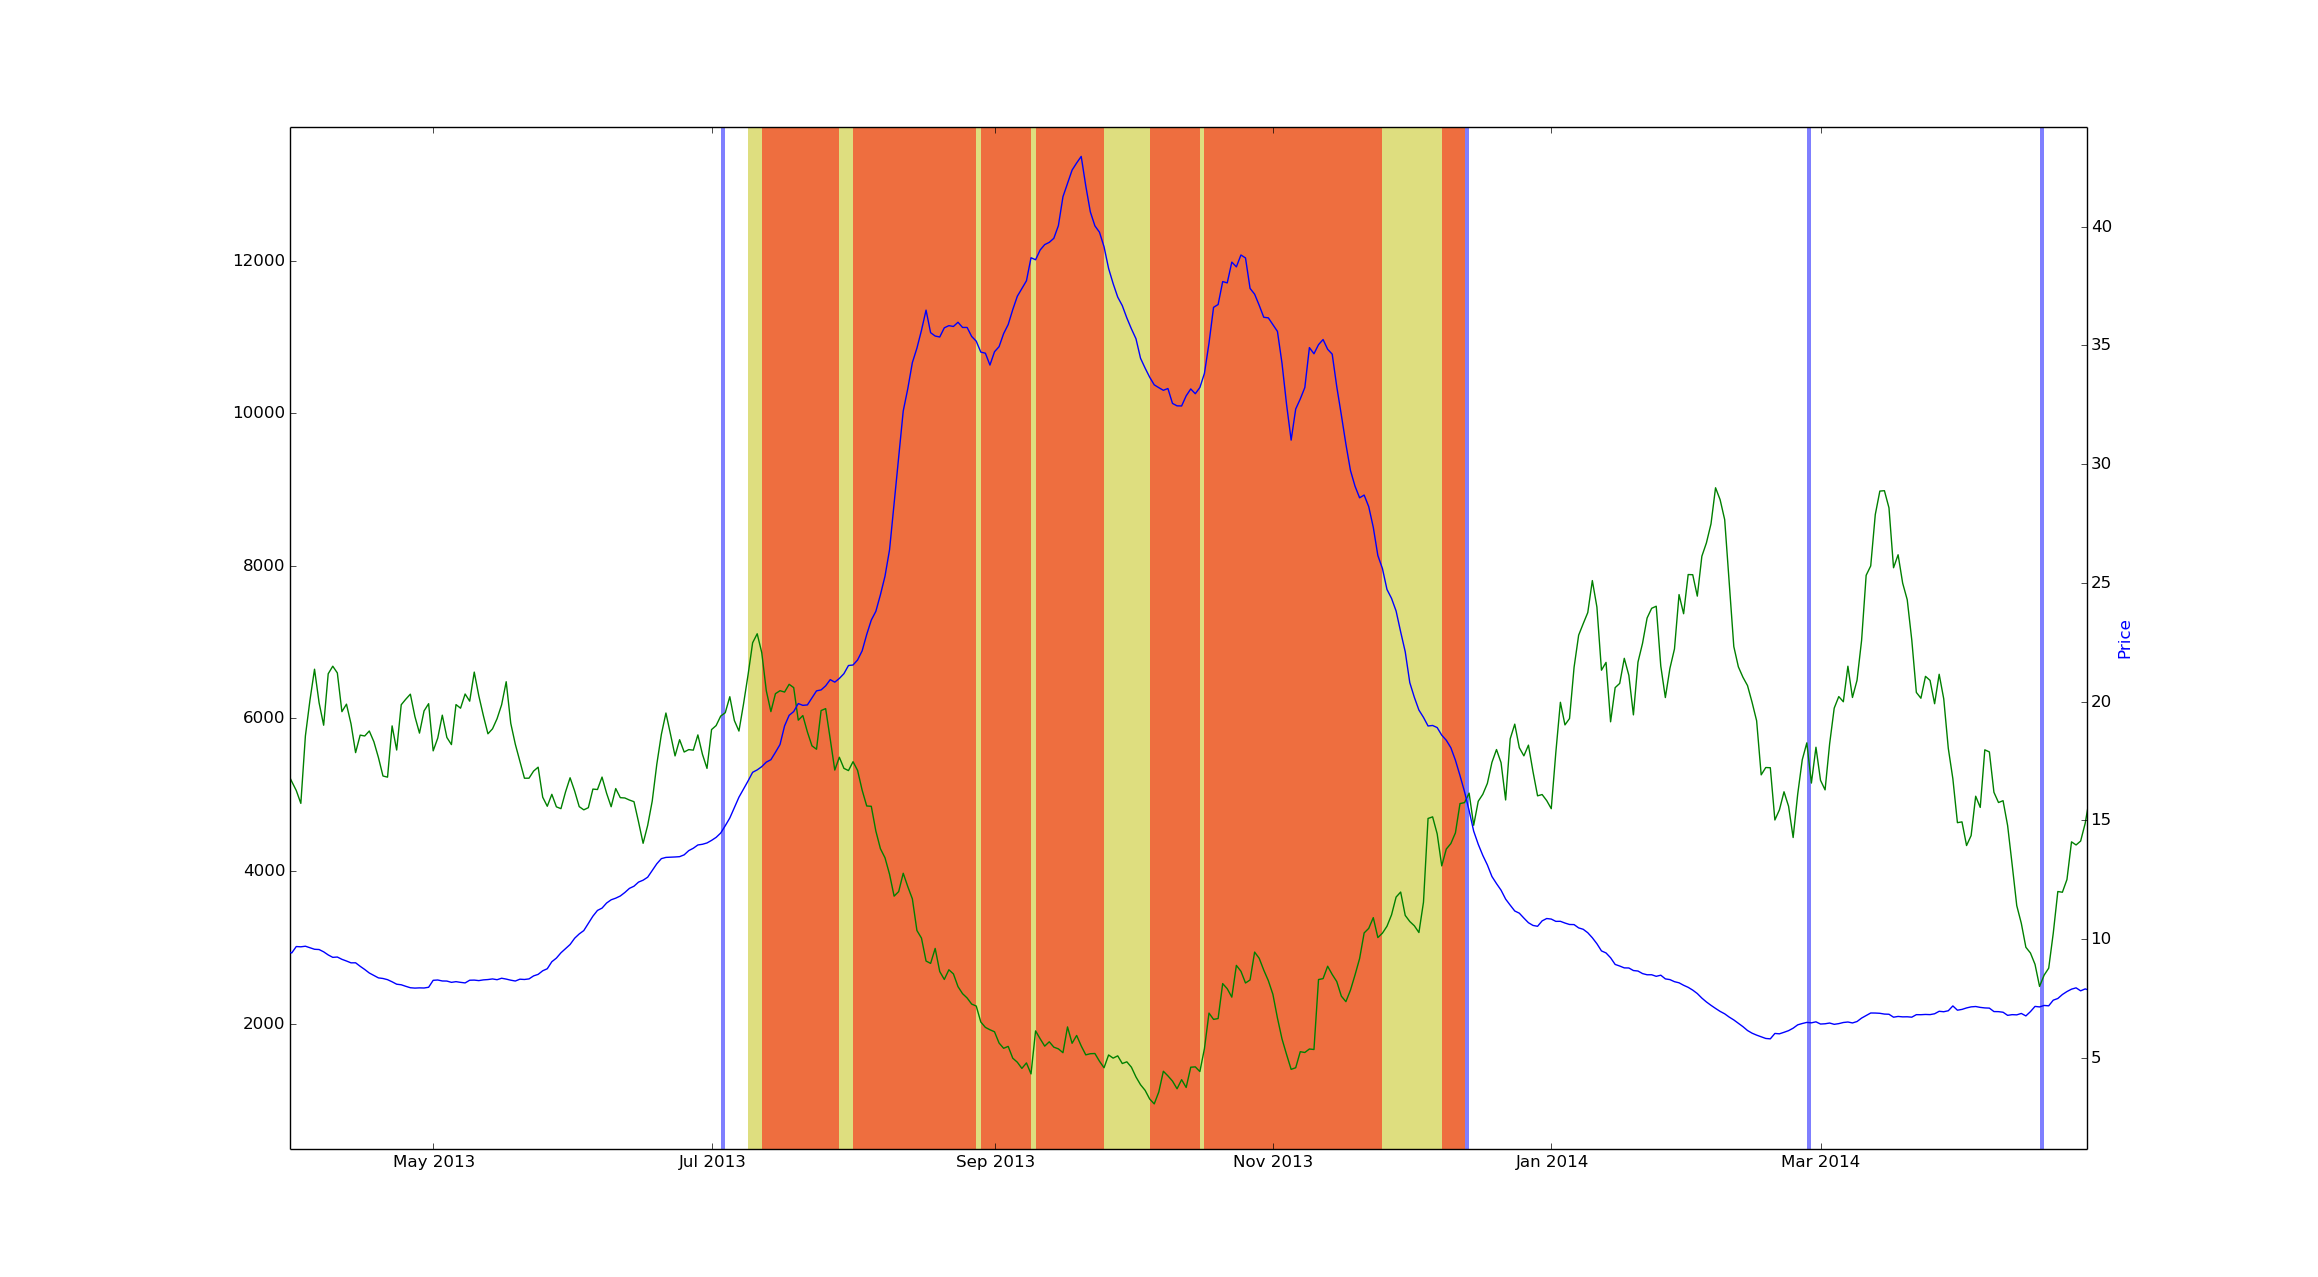
\includegraphics[width=0.8\textwidth]{graphs/12241.png}
		    	\caption{Linear Regression (Green line - Arrival Data of Onion, Blue Line - Wholesale Price)}
		    	\label{fig:12241}
			\end{figure}
			
			
			
			\item Now, this method has also missed few of the articles for this analysis as well. Now, looking at the graphs we could not interpret what may be exact reason why they were missed. But method may have found prices to be moderate and that's why they might have been missed.
			
			Following tenures are some cases reported by this method:
			\begin{itemize}
				\item \textit{Analysis 2}: Jan Feb 2013, July 2014, June July 2015 (See Figure \ref{fig:12222})
				\item \textit{Analysis 4}: Jan Feb 2013, June July 2013, June 2015 (See Figure \ref{fig:12242})
			\end{itemize}
			\begin{figure}[H]
		    	\centering
  		    	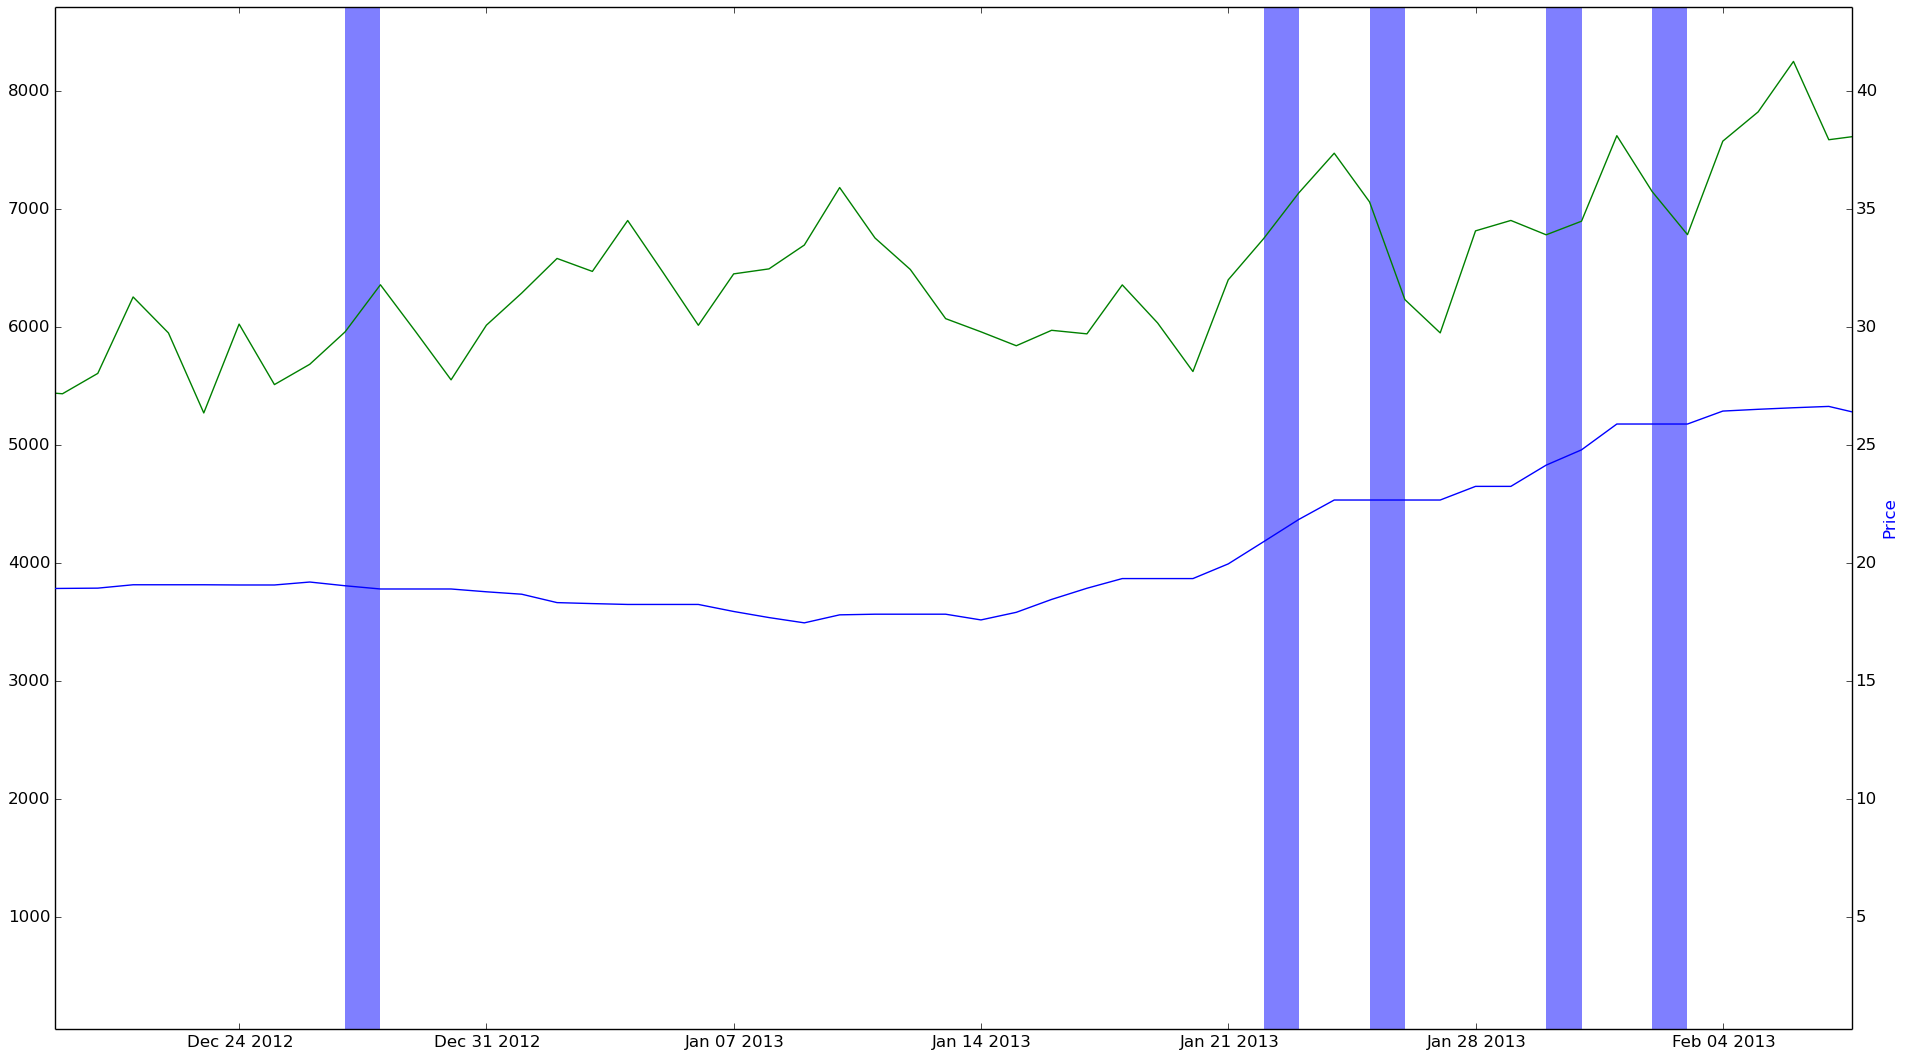
\includegraphics[width=0.8\textwidth]{graphs/12222.png}
		    	\caption{Linear Regression (Green line - Arrival Data of Onion, Blue Line - Retail Price)}
		    	\label{fig:12222}
			\end{figure}
			
			\begin{figure}[H]
		    	\centering
  		    	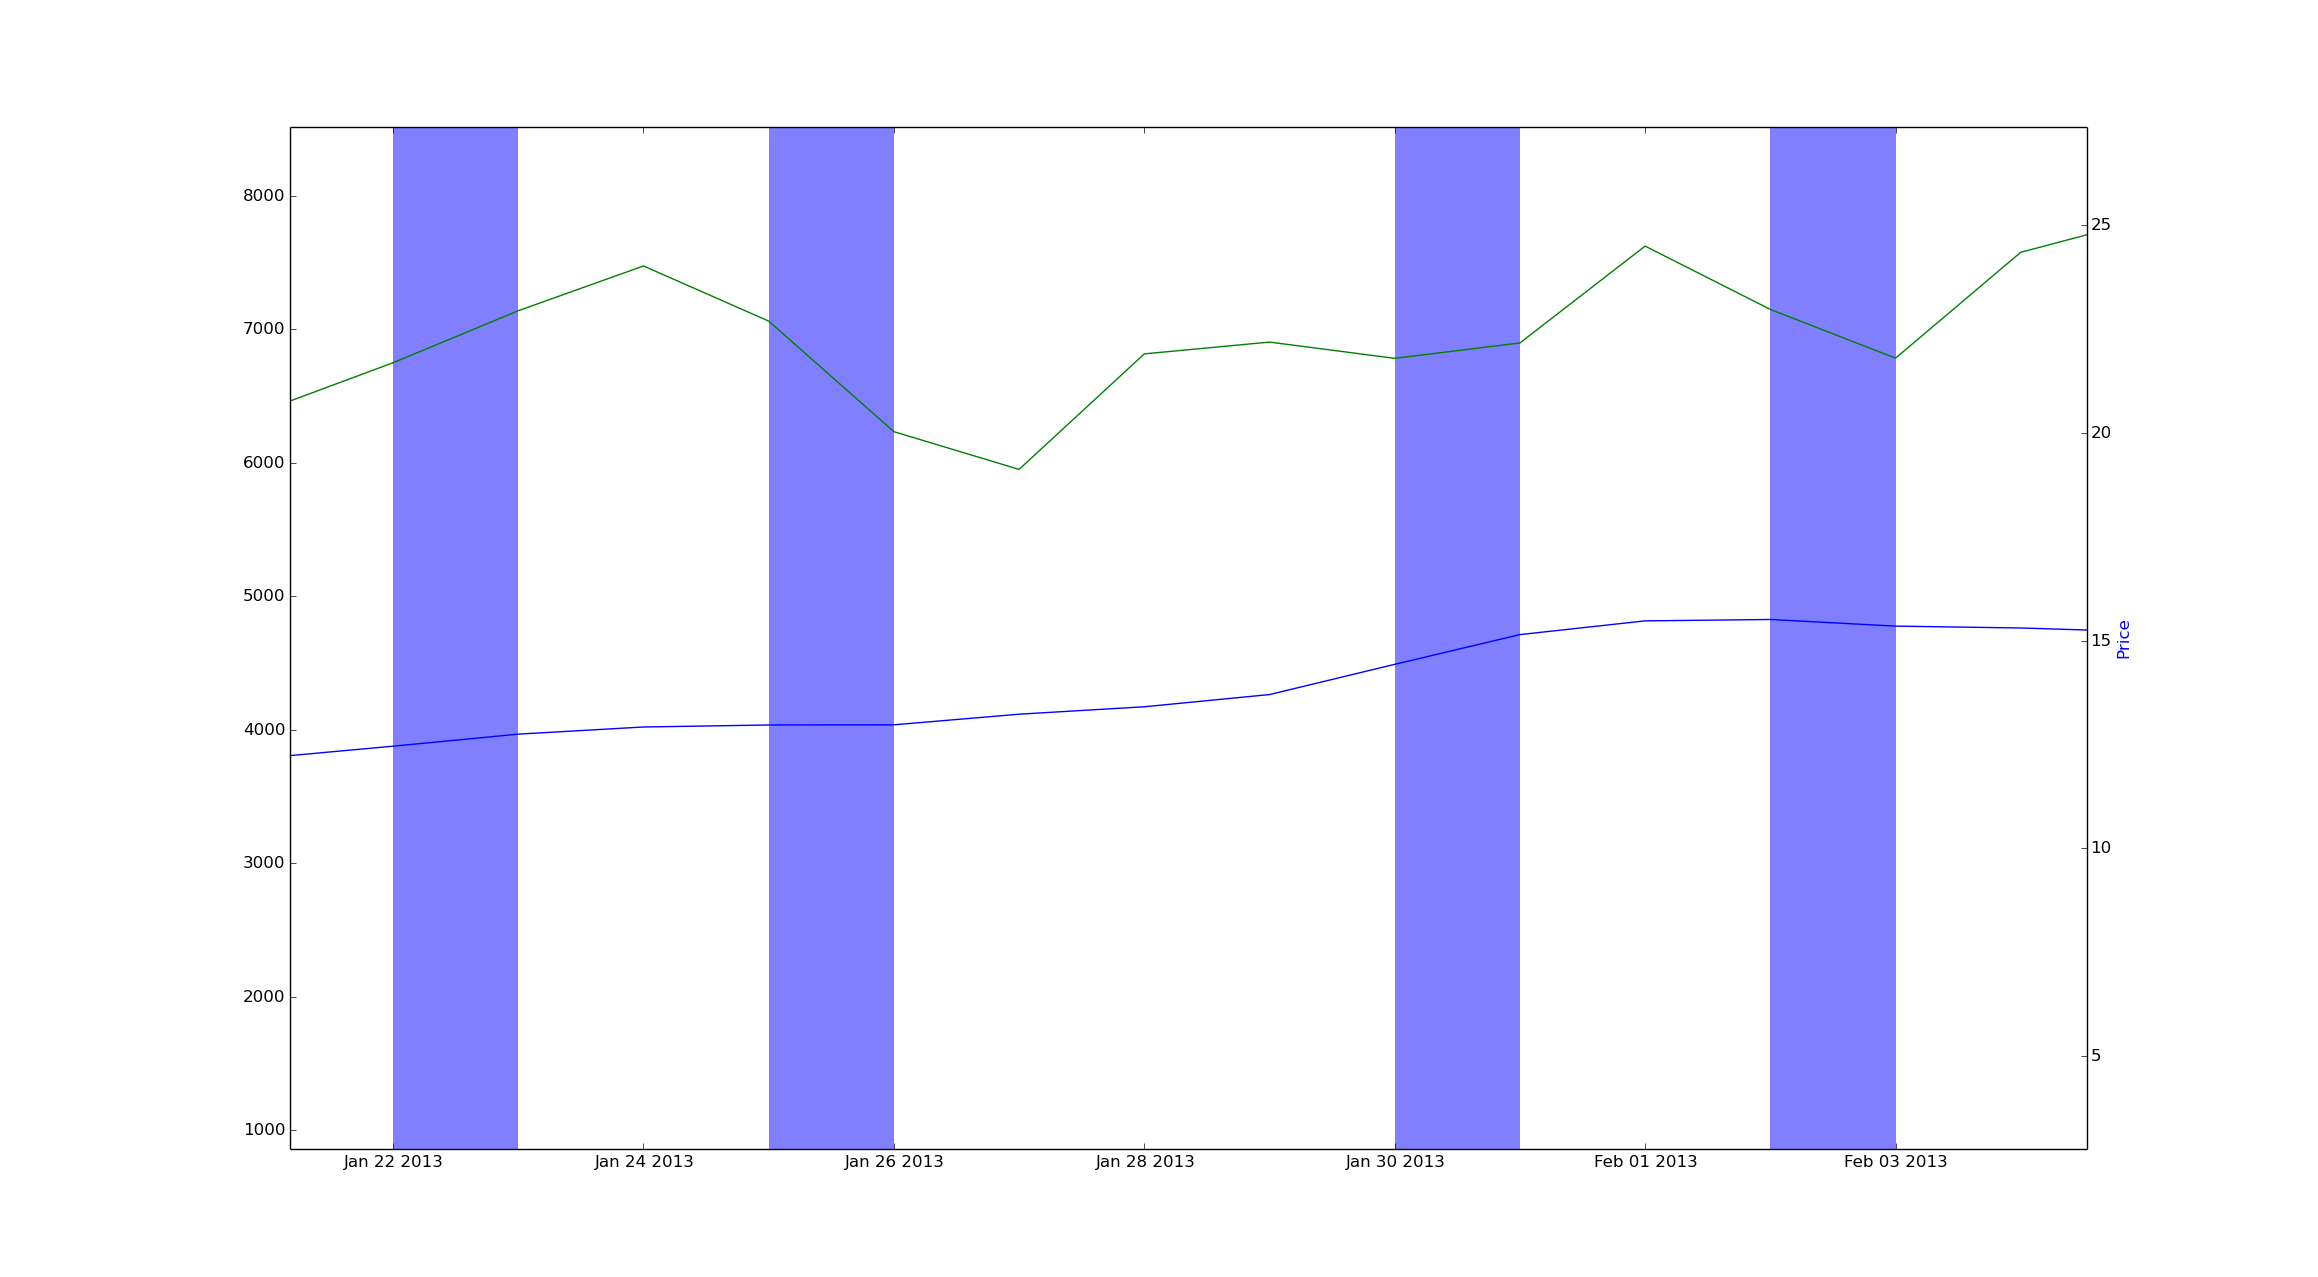
\includegraphics[width=0.8\textwidth]{graphs/12242.png}
		    	\caption{Linear Regression (Green line - Arrival Data of Onion, Blue Line - Wholesale Price)}
		    	\label{fig:12242}
			\end{figure}
		\end{itemize}

		
\subsection{Window Based Correlation}

		This method checks if the provided two timeseries moves in tandem or not. If not, then what are the time periods when they are not following the desired behavior. In order to find such time periods in the timeseries, the whole timeseries is divided into smaller windows and correlation value computed for that window is used to determine if that period is anomalous or not. The P-value of 0.01 is used in order to check the significance of correlation value.
		\\
		\\
		The function is tested with different set of timeseries. Following are the four tests which were performed:
		\begin{enumerate}
			\item \textbf{Retail Price vs Average of Retail Price}: This test tries to find if any centre deviates from other centres abruptly. Average of timeseries of all the centres is taken as a representative timeseries for the behavior of all the centres which is compared with every centre in order to find time periods where these two did not move in tandem
			\item \textbf{Retail Price vs Arrival of Onion}: Retail timeseries is expected not to move in tandem with Arrival timeseries. So, the time periods with positive correlation values are spotted in this. 
			\item \textbf{Retail Price vs Wholesale Price}: Retail timeseries is expected to move in tandem with wholesale timeseries. So, the time periods with negative correlation values are spotted in this.
			\item \textbf{Wholesale Price vs Arrival of Onion}: Wholesale timeseries is expected to not move in tandem with Arrival timeseries. So, the time periods with positive correlation values are spotted in this. 
		\end{enumerate}
		
		The two timeseries are first aligned with each other at the maximum lag value. Then the entire timeseries is divided into small time periods of 15 days in order to locate anomalous situations through their respective correlation values.
		\\
		\\
		Observations when retail price timeseries is compared with average of retail price timeseries: 
		
		\begin{itemize}
			\item The timeseries showed the initial shift/lag of zero days which means both the timeseries are best aligned without any lag.
			
			Some of the tenures for which the method reported anomalies are:
			
			\begin{itemize}
				\item 2008-03-06 to 2008-03-20 (See Figure \ref{fig:20080306_0320})
				\item 2009-09-12 to 2009-09-26 (See Figure \ref{fig:20090912_0926})
				\item 2011-07-04 to 2011-08-02 (See Figure \ref{fig:20110704_0802})
			\end{itemize}
			\begin{figure}[H]
		    	\centering
  		    	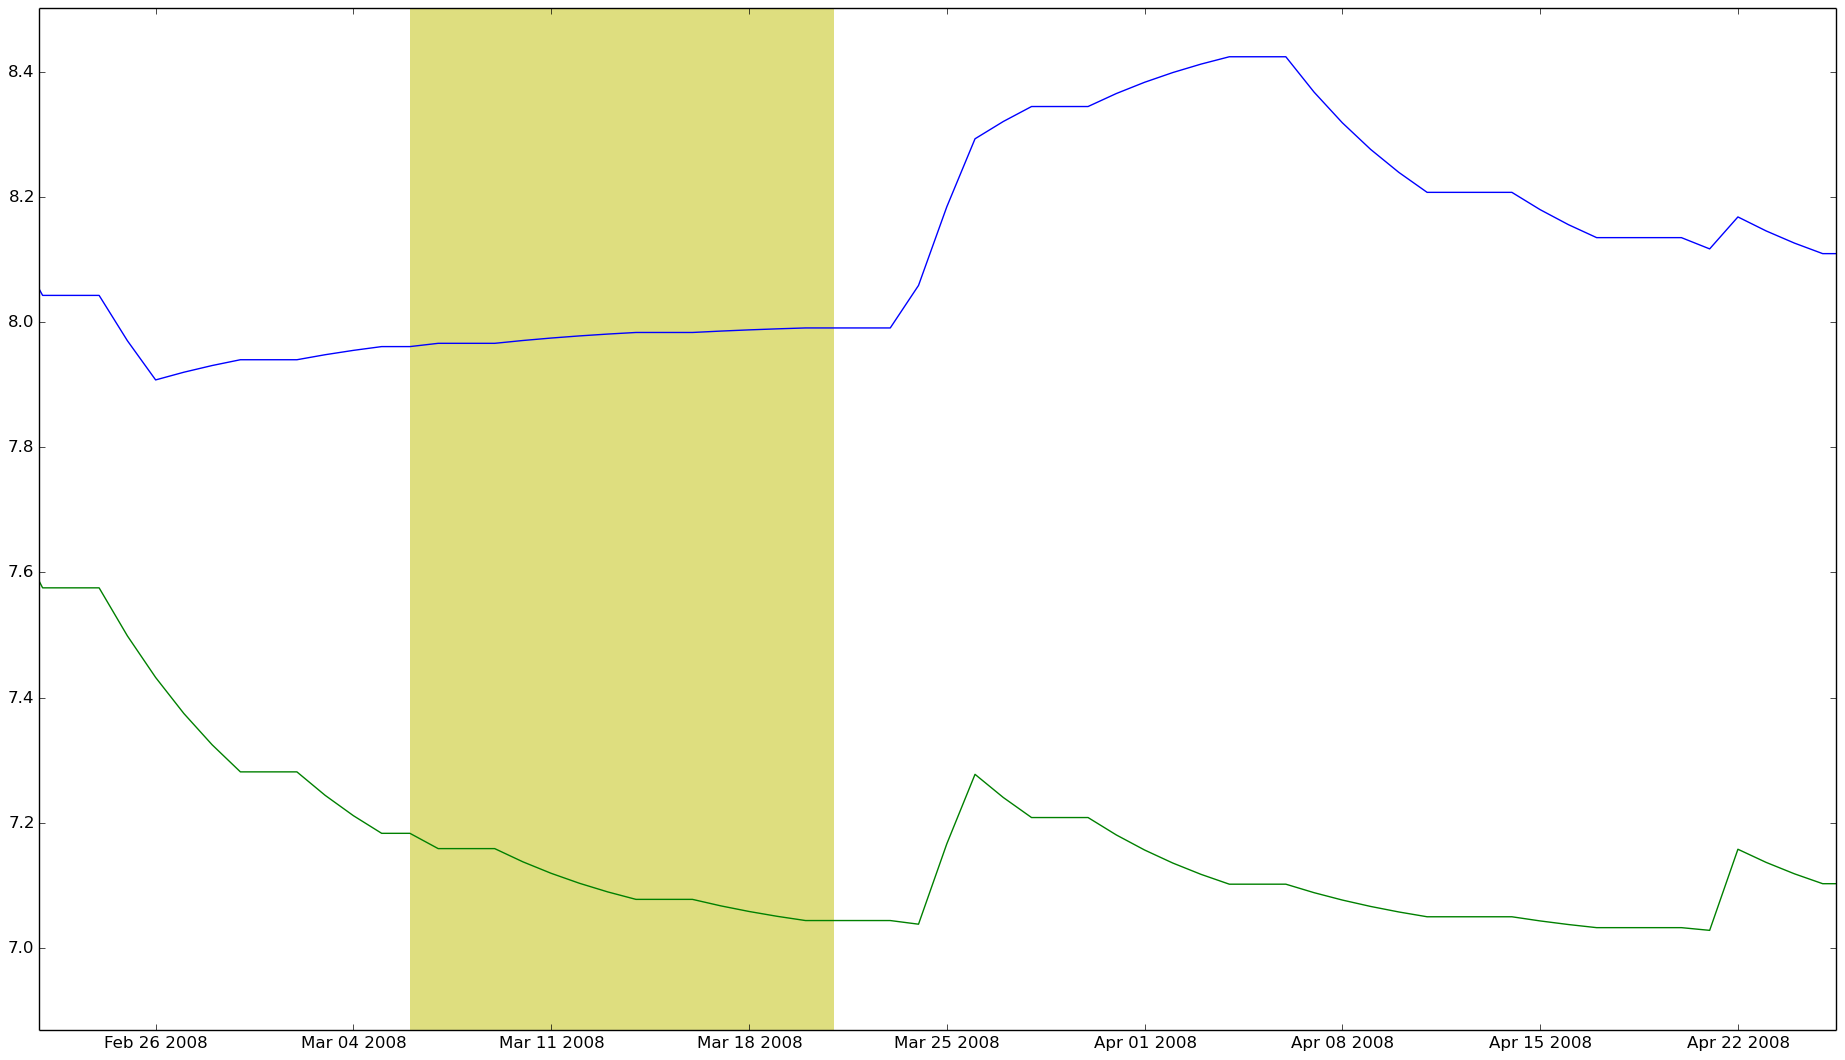
\includegraphics[width=0.8\textwidth]{graphs/20080306_0320.png}
		    	\caption{Window based correlation (Green line - Centre Retail Price, Blue Line - Average Retail Price)}
		    	\label{fig:20080306_0320}
			\end{figure}
			
			\begin{figure}[H]
		    	\centering
  		    	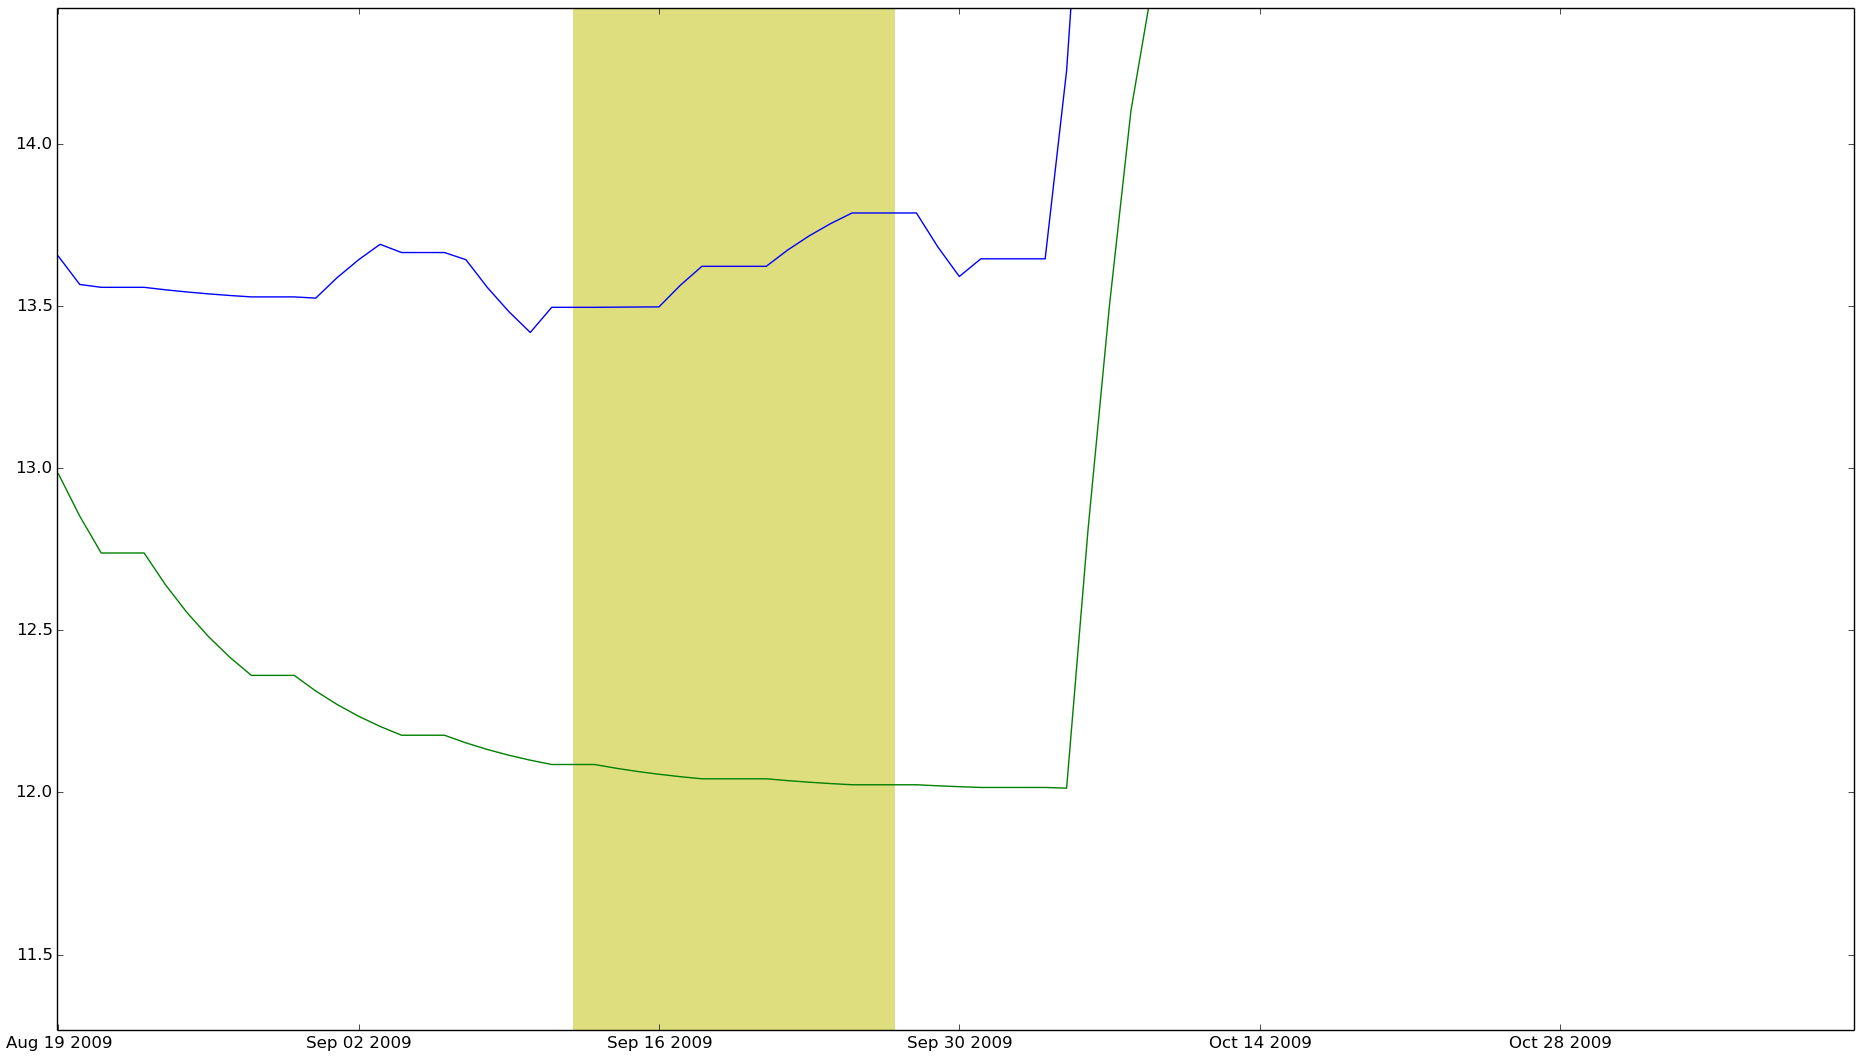
\includegraphics[width=0.8\textwidth]{graphs/20090912_0926.png}
		    	\caption{Window based correlation (Green line - Centre Retail Price, Blue Line - Average Retail Price)}
		    	\label{fig:20090912_0926}
			\end{figure}

			\begin{figure}[H]
		    	\centering
  		    	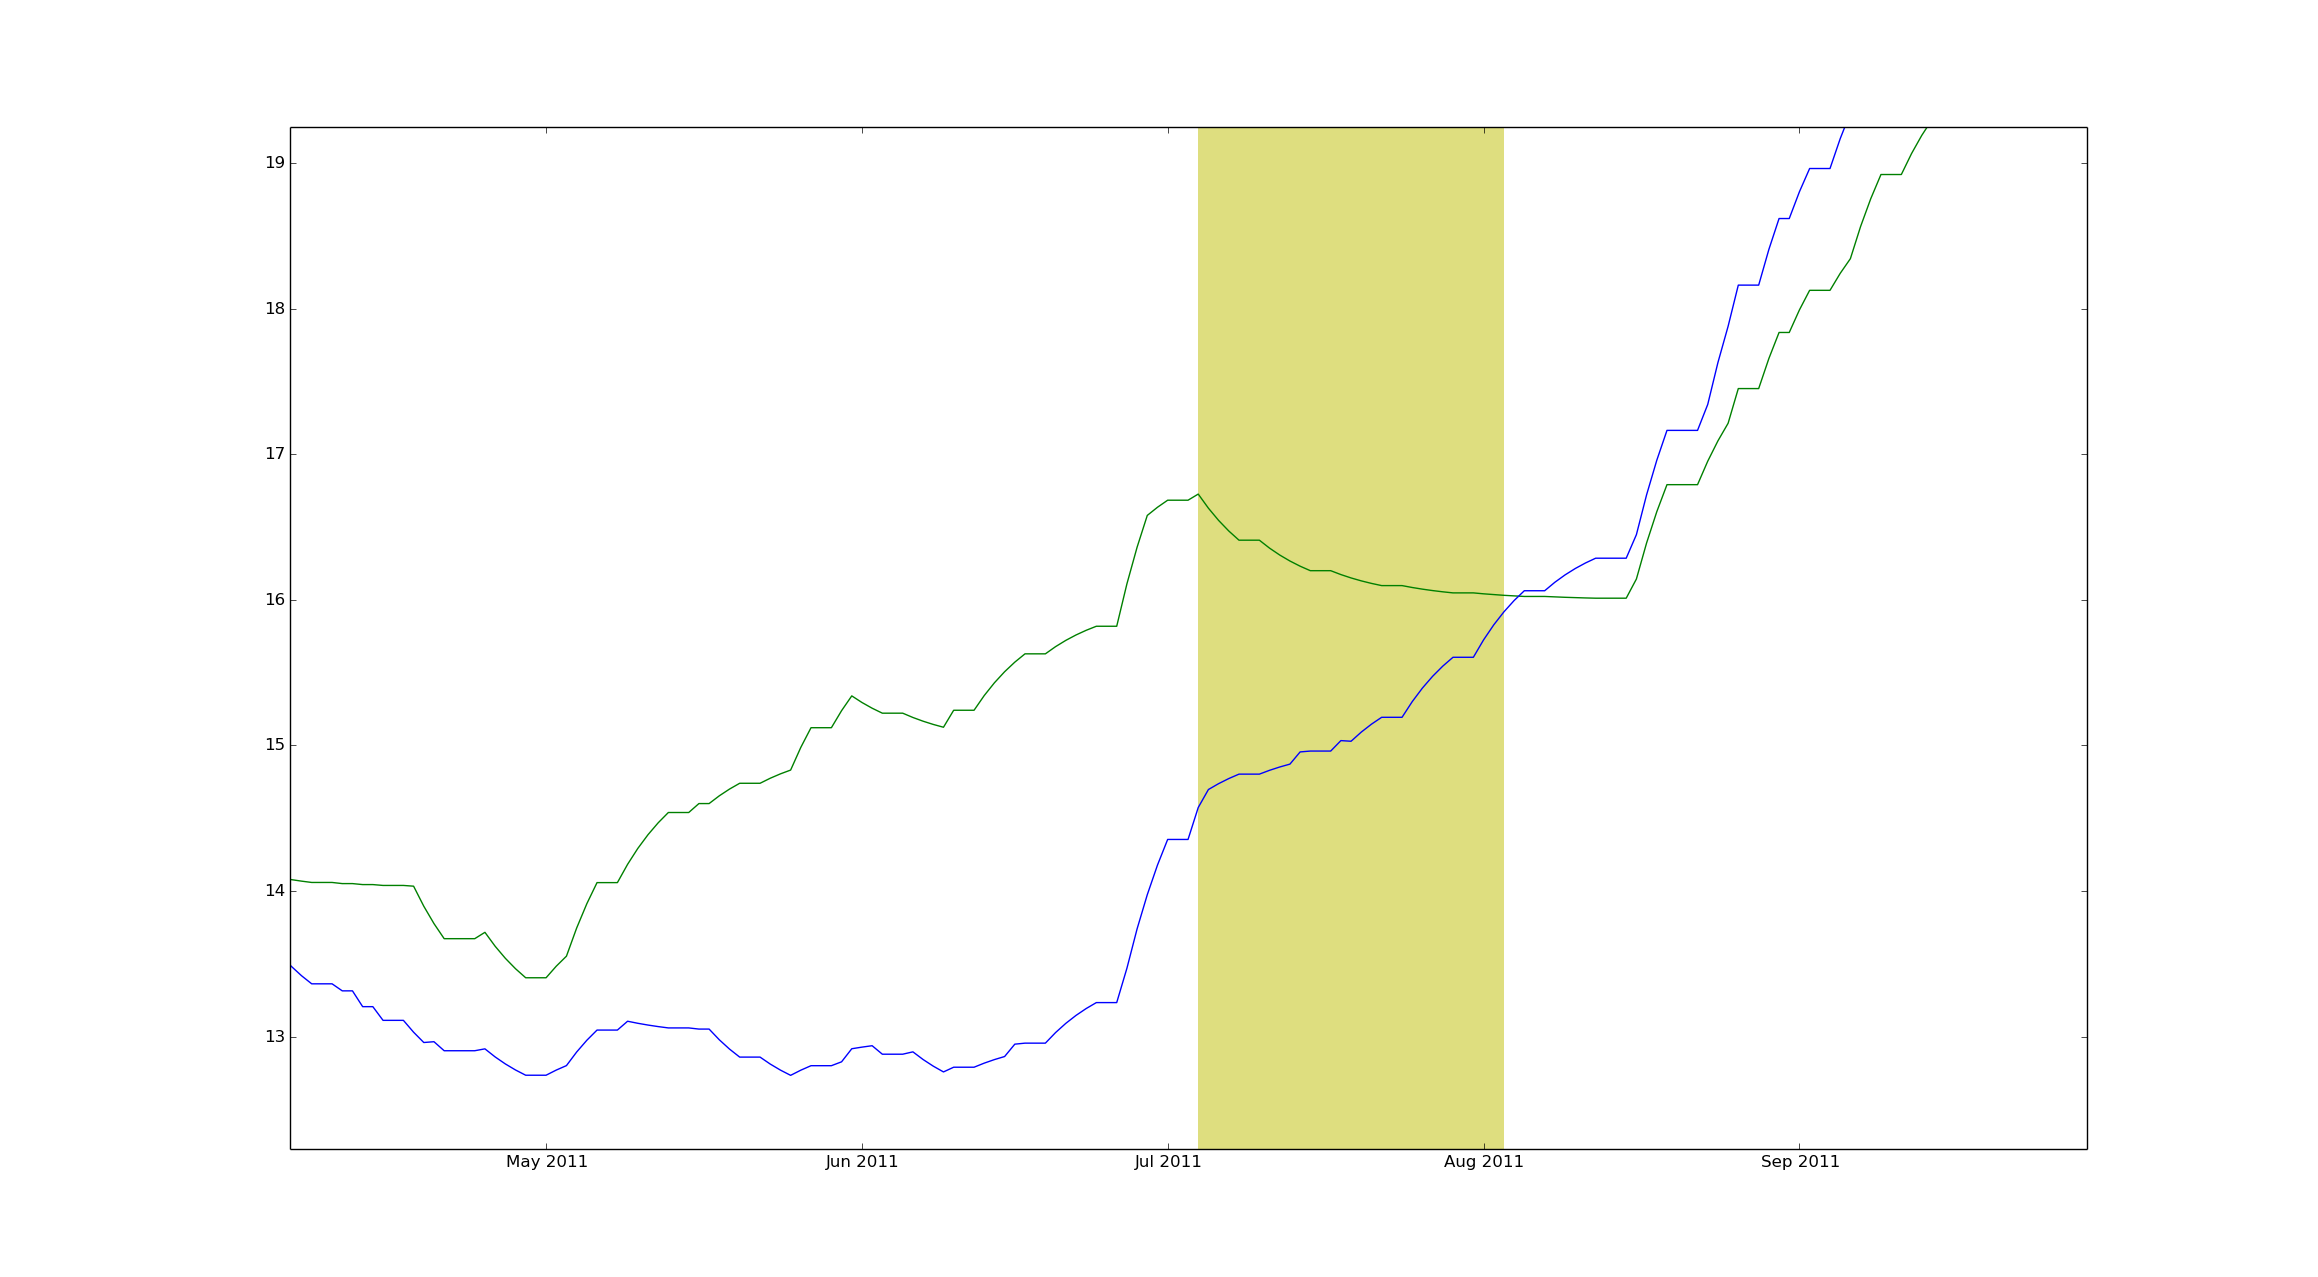
\includegraphics[width=0.8\textwidth]{graphs/20110704_0802.png}
		    	\caption{Window based correlation (Green line - Centre Retail Price, Blue Line - Average Retail Price)}
		    	\label{fig:20110704_0802}
			\end{figure}
			
			But looking closely in the data, it is found that these tenures are reported because the two series were not in tandem which was mostly because prices of delhi faced some fluctuations whereas Mumbai prices did not show evident fluctuations. One of the reason for fluctuation in prices of Delhi over Mumbai could be because Delhi is dependent on other states for Onion whereas Mumbai does not have such issue.
			\\
			\\
			Some of the tenures which went unnoticed by method:
			
			\begin{itemize}
				\item 2010-12-20 to 2010-12-25 (See Figure \ref{fig:20101220_1225})
				\item 2011-01-06 to 2011-01-08 (See Figure \ref{fig:20110106_0108})
				\item 2012-12-27 to 2013-01-05 (See Figure \ref{fig:20121227_0105})
			\end{itemize}
			\begin{figure}[H]
		    	\centering
  		    	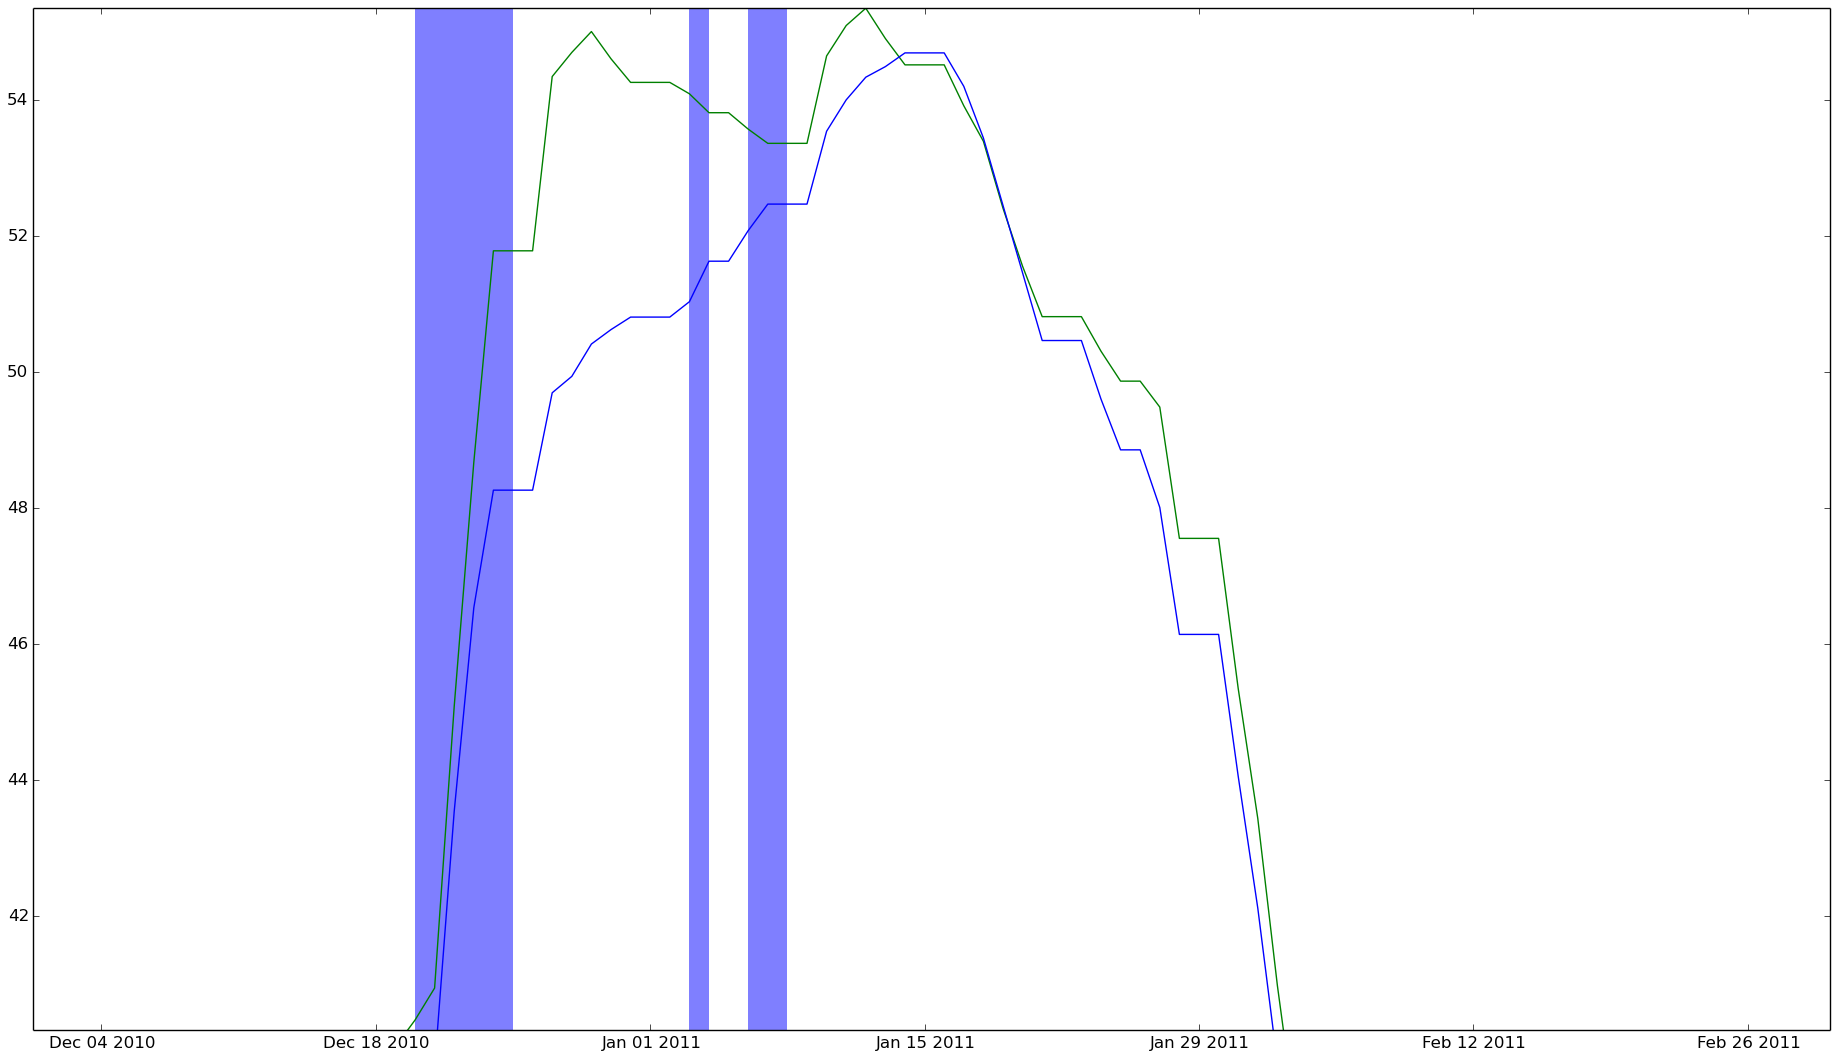
\includegraphics[width=0.8\textwidth]{graphs/20101220_1225.png}
		    	\caption{Window based correlation (Green line - Centre Retail Price, Blue Line - Average Retail Price)}
		    	\label{fig:20101220_1225}
			\end{figure}
			
			\begin{figure}[H]
		    	\centering
  		    	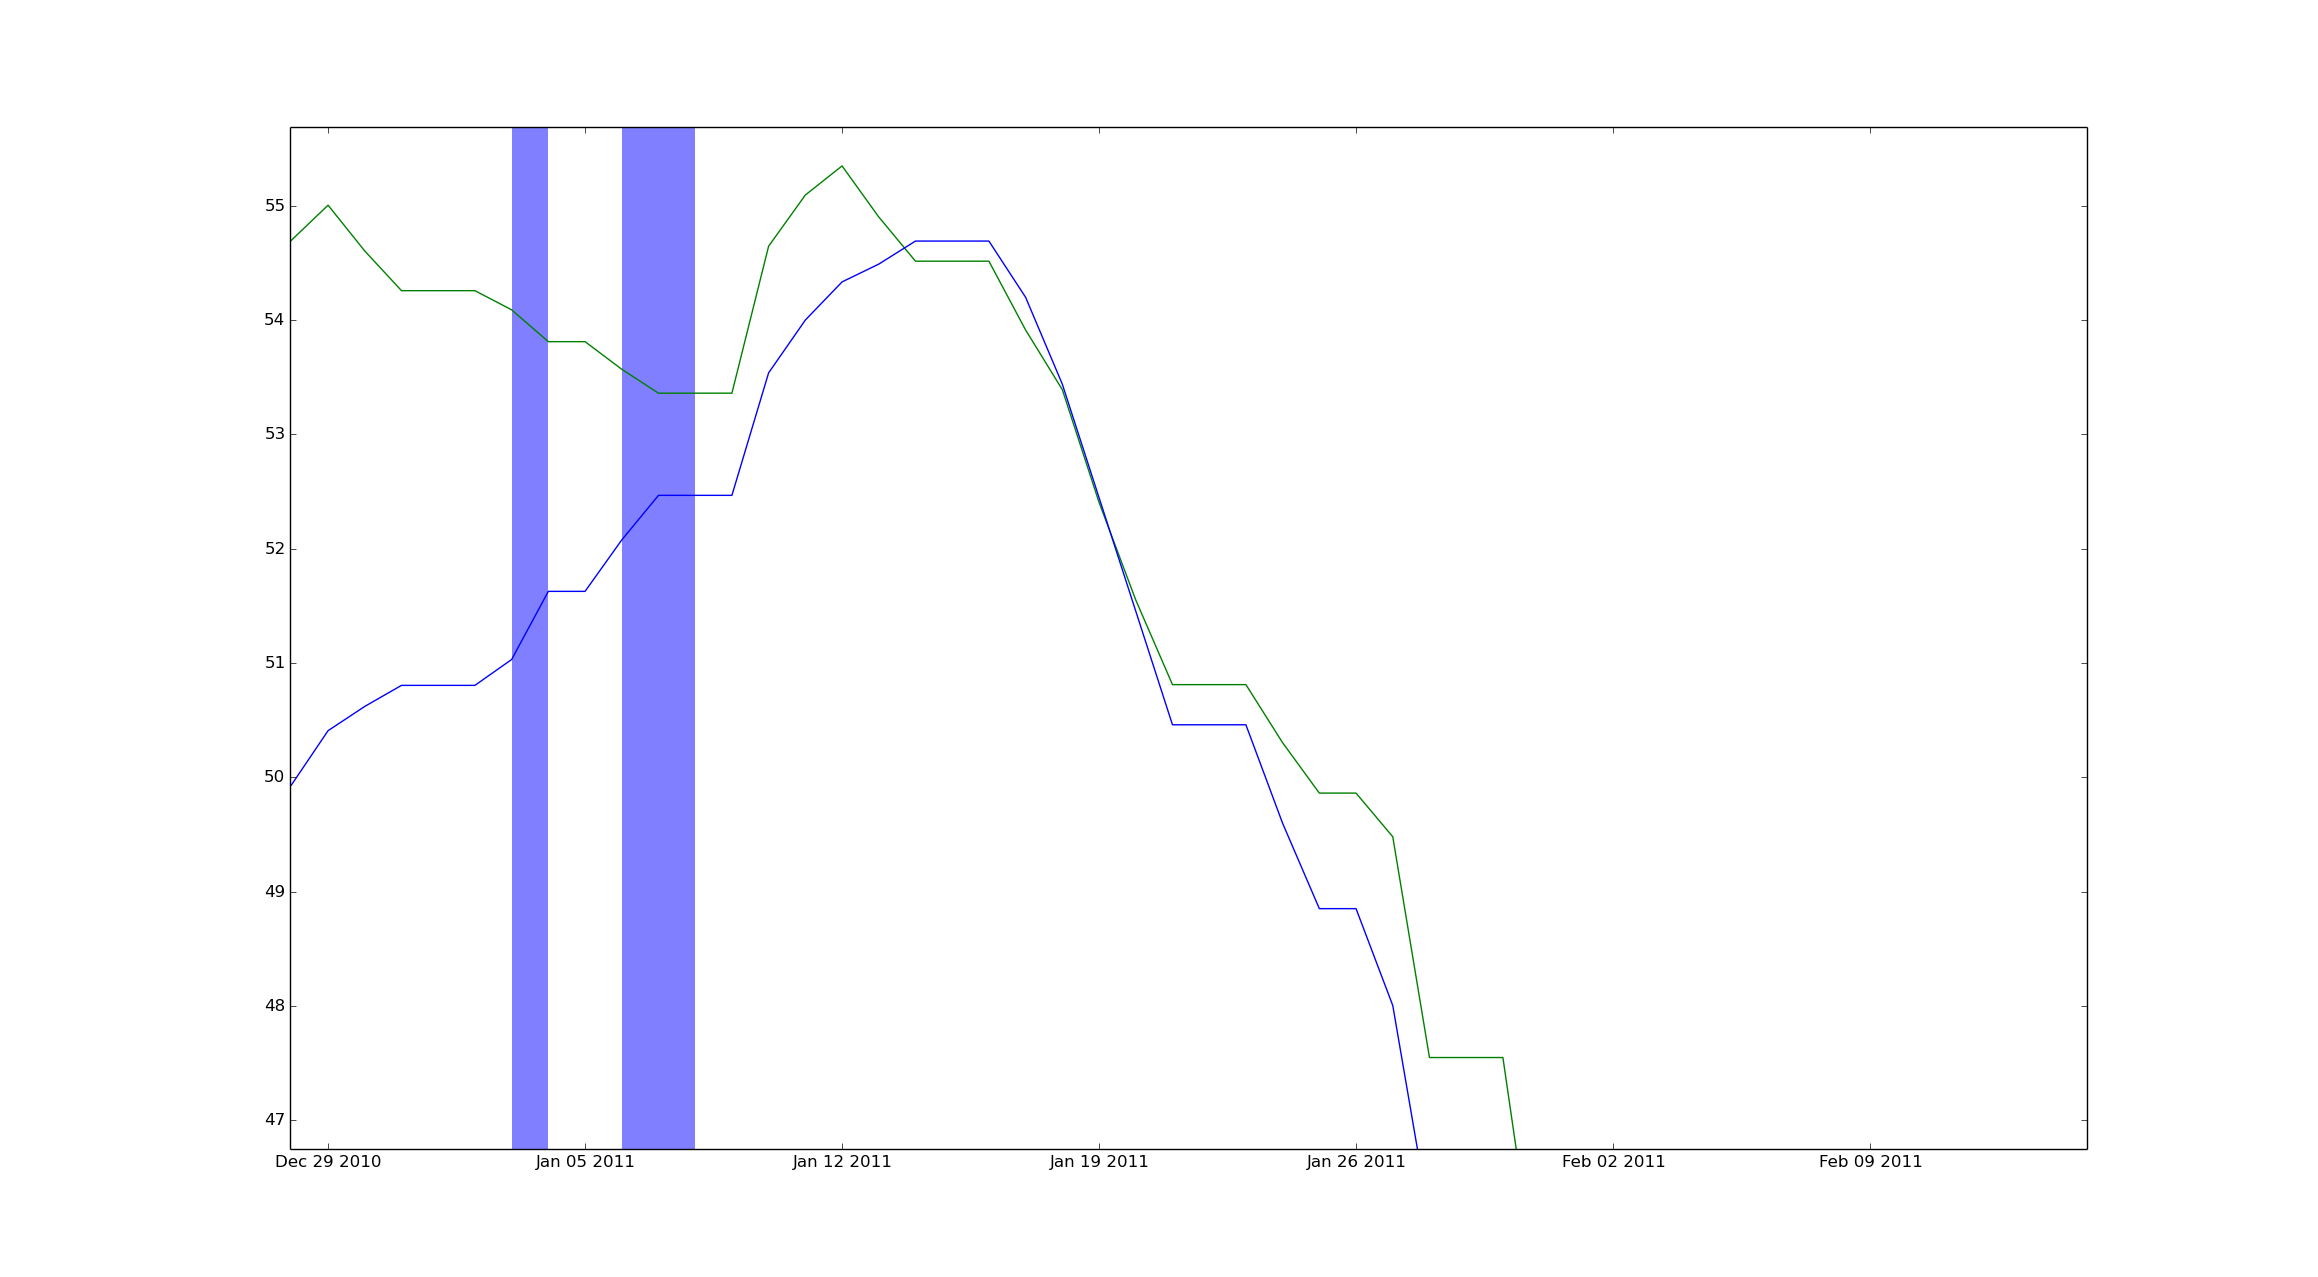
\includegraphics[width=0.8\textwidth]{graphs/20110106_0108.png}
		    	\caption{Window based correlation (Green line - Centre Retail Price, Blue Line - Average Retail Price)}
		    	\label{fig:20110106_0108}
			\end{figure}

			\begin{figure}[H]
		    	\centering
  		    	\includegraphics[width=0.8\textwidth]{graphs/20121227_0105.png}
		    	\caption{Window based correlation (Green line - Centre Retail Price, Blue Line - Average Retail Price)}
		    	\label{fig:20121227_0105}
			\end{figure}
			
			Some of the tenures which were reported by news reports as well as method:
			
			\begin{itemize}
				\item 2013-10-06 to 2013-10-15 (See Figure \ref{fig:20131006_1015_1021})
				\item 2013-10-17 to 2013-10-21 (See Figure \ref{fig:20131006_1015_1021})
			\end{itemize}
			\begin{figure}[H]
		    	\centering
  		    	\includegraphics[width=0.8\textwidth]{graphs/20131006_1015_1021.png}
		    	\caption{Window based correlation (Green line - Centre Retail Price, Blue Line - Average Retail Price)}
		    	\label{fig:20131006_1015_1021}
			\end{figure}
						
		\end{itemize}
		
		Other interesting observations that were found while conducting above mentioned tests are as following:
		\begin{itemize}
			\item The lag chosen while comparing retail and arrival for Mumbai came as 15 days which means it takes 15 days of time for arrival to impact retail.
			\item The lag chosen by method while comparing retail and arrival for Delhi came out to be -9 days which gives hints that retail prices are impacting arrival of Onion which is not ideal in real time scenario.
			\item The lag chosen while comparing retail and wholesale for Mumbai comes out as -15 which means retail prices are impacted in approx. 15 days after change in the wholesale prices.
			\item The lag chosen while comparing retail and wholesale for Delhi comes out as -4 which is clearly very small than Mumbai. It might be because of smaller supply chain in Delhi compared to Mumbai.
			\item The lag chosen while comparing wholesale and arrival for Mumbai came as 11 days which means it takes 11 days of time for arrival to impact wholesale.
			\item The lag chosen by method while comparing wholesale and arrival for Delhi came out to be -14 days which gives hints that wholesale prices are impacting arrival of Onion which is not ideal in real time scenario.
		\end{itemize}
		
		Limitations of method:
		\begin{itemize}
			\item The method reports all the tenures where series are not in sync or are in sync(as needed). Like in case of  2008-03-06 to 2008-03-20 for retail vs average, though the correlation went really high because of opposite directions but the fluctuation in prices were not very prominent.
			\item If all the timeseries follows same anomalous behavior then it is not possible to find anomaly in any.
			\item If the anomaly is for very small tenure compared to the selected window size then it is likely to be missed or go unnoticed. In case of 2011-01-06 - 2011-01-08
		\end{itemize}

\subsection{Multivariate Time Series- Vector Autoregressive}

		The method uses vector autoregressive framework for multivaraiate time-series analysis in order to forecast values by using all the related variables/timeseries that can impact the timeseries. The error in the predicted value with the original value helps in determining anomalous points from the timeseries. MAD test is applied in order to fix the threshold value for the error.
		60\% (This can be configured as per need) of the data is used for calibration and rest of the data is checked for anomalous points. So, the start date for the anomalous points begins after 2011-09-16
		\\
		The function is tested with different set of timeseries. Following are the four tests which were performed:
		\begin{enumerate}
		    \item \textbf{Retail Price vs Average of Retail Price}: All the centres should ideally move in tandem. So test is performed over every centre with other centres helping in predicting values.            
		    \item \textbf{Retail Price vs Arrival of Onion}: Arrival is one of the major deciding factor for retail. So the predictions are made for retail based on arrival.
		    \item \textbf{Retail Price vs Wholesale Price}: Retail prices are predicted based on the wholesale prices.
		    \item \textbf{Wholesale Price vs Arrival of Onion}: Wholesale timeseries is predicted on the basis of arrival timeseries.
		\end{enumerate}
		
		Observations when retail price timeseries is compared with average of retail price timeseries: 
		
		\begin{itemize}
			\item The threshold selected by this method for error values are -19.0358099572 and 107.697818954 which means all the data points with error values less than -19.0358099572 and greater than 107.697818954 are reported by the method.
			
			Some of the tenures for which the method reported anomalies are:
			
			\begin{itemize}
				\item 2013-07-19 to 2013-09-11 (See Figure \ref{fig:20130719_0911})
				\item 2013-09-17 to 2014-01-06 (See Figure \ref{fig:20130917_0106})
				\item 2014-12-03 to 2014-12-15 (See Figure \ref{fig:20141203_1215})
			\end{itemize}
			\begin{figure}[H]
		    	\centering
  		    	\includegraphics[width=0.8\textwidth]{graphs/20130719_0911.png}
		    	\caption{Vector Autoregressive (Green line - Centre Retail Price, Blue Line - Average Retail Price)}
		    	\label{fig:20130719_0911}
			\end{figure}
			
			\begin{figure}[H]
		    	\centering
  		    	\includegraphics[width=0.8\textwidth]{graphs/20130917_0106.png}
		    	\caption{Vector Autoregressive (Green line - Centre Retail Price, Blue Line - Average Retail Price)}
		    	\label{fig:20130917_0106}
			\end{figure}

			\begin{figure}[H]
		    	\centering
  		    	\includegraphics[width=0.8\textwidth]{graphs/20141203_1215.png}
		    	\caption{Vector Autoregressive (Green line - Centre Retail Price, Blue Line - Average Retail Price)}
		    	\label{fig:20141203_1215}
			\end{figure}
			
			No data points were reported against news articles present in May, June, July 2014 despite of large error value. The threshold selected by the MAD test was higher than the error values. This could be corrected by manually setting threshold values which can be account for these data points.
			
		\end{itemize}
		
		Other interesting observations that were found while conducting above mentioned tests are as following:
		\begin{itemize}
			\item Some of the data points like July 2014 data were not captured despite of error value close to MAD threshold. These can be captured by lowering the threshold.
			\item For news articles in Dec 2012,Jan 2013, Feb 2013 the values does not show high error values despite of news articles reporting the crisis. The possible reason could be because similar trend have been seen for this tenure in the data.
		\end{itemize}
		
		Limitations of method:
		\begin{itemize}
			\item The method depends on the MAD Test in order to set threshold. So, even though the error value is close to threshold but less than it won't be reported. Other methods could be also used in order to decide threshold.
		\end{itemize}		
		
		
\subsection{Graph Based Anomaly Detection}

	This method, treats each day as a node of a graph, and connects with other nodes if nodes are similar. This connecting edge is given similarity value and random walk is performed to get connectivity of each node. Node with the least connectivity values are reported as anomaly. Note that for the previous methods, we had threshold values either defined by user or calculated by using MAD test. But here we do not have that and we just ask method to report "n" number of nodes with least connectivity values.\\
	\\
	The working of this method is quite complex and can not be generalised. For detailed information go through the paper. So we will just represent, how method has performed on the different analysis.\\
	\\
	For \textbf{Retail Price vs Average of Retail Price} (See Figure \ref{fig:1231}) and \textbf{Retail Price vs Wholesale Price} (See Figure \ref{fig:12331}), this method has performed well. For \textbf{Retail Price vs Average of Retail Price}, every tenure of anomaly has been matched with some news articles.
	\\
	The anomalies which were not matched with news articles were part of large tenure which had some matching with news articles and usually, this tenure is large and for every date news articles are not present. 
	\\
	Few articles are missed, that might be due to limited number of points chosen. If number of points are increased, than it might be covered as well. 
	\\
	For \textbf{Retail Price vs Wholesale Price}, apart from Jan 2013, July 2014, June 2015, all anomalies are matching with some news articles.\\
			\begin{figure}[H]
		    	\centering
  		    	\includegraphics[width=0.8\textwidth]{graphs/1231.png}
		    	\caption{Graph Based Anomaly Detection (Green line - Centre Retail Price, Blue Line - Average Retail Price)}
		    	\label{fig:1231}
			\end{figure}
			
			\begin{figure}[H]
		    	\centering
  		    	\includegraphics[width=0.8\textwidth]{graphs/12331.png}
		    	\caption{Graph Based Anomaly Detection (Green line - Retail Price, Blue Line - Wholesale Price)}
		    	\label{fig:12331}
			\end{figure}
	
	For \textbf{Retail Price vs Arrival of Onion} (See Figure \ref{fig:12321}) and \textbf{Wholesale Price vs Arrival of Onion} (See Figure \ref{fig:12341}), this method is not producing good results. Many points are reported as anomaly which are close to each other. And due to limited number of points, number of anomalies matching with news articles are quite less. The reason might be because of fluctuations seen in the arrival timeseries. Figures \ref{fig:12322_delhi} and \ref{fig:12442_delhi} describe results of these both analysis for Delhi centre.
			\begin{figure}[H]
		    	\centering
  		    	\includegraphics[width=0.8\textwidth]{graphs/12321.png}
		    	\caption{Graph Based Anomaly Detection (Green line - Arrival Data of Onion, Blue Line - Retail Price)}
		    	\label{fig:12321}
			\end{figure}
			
			\begin{figure}[H]
		    	\centering
  		    	\includegraphics[width=0.8\textwidth]{graphs/12341.png}
		    	\caption{Graph Based Anomaly Detection (Green line - Arrival Data of Onion, Blue Line - Wholesale Price)}
		    	\label{fig:12341}
			\end{figure}
			
			
			\begin{figure}[H]
		    	\centering
  		    	\includegraphics[width=0.8\textwidth]{graphs/12322_delhi.png}
		    	\caption{Graph Based Anomaly Detection (Green line - Arrival Data of Onion, Blue Line - Retail Price)}
		    	\label{fig:12322_delhi}
			\end{figure}
			
			\begin{figure}[H]
		    	\centering
  		    	\includegraphics[width=0.8\textwidth]{graphs/12442_delhi.png}
		    	\caption{Graph Based Anomaly Detection (Green line - Arrival Data of Onion, Blue Line - Wholesale Price)}
		    	\label{fig:12442_delhi}
			\end{figure}	

\chapter{Results and Findings}

The analysis was performed for different time-series of two centers- Delhi and Mumbai.

Following analysis is for Mumbai. In case of Mumbai, there are total of 66 distinct days for which news articles exist. Here, articles not matched represents unique dates for which articles were present but system failed to report anomaly against that date.
\begin{table}[H]
\centering

\begin{tabular}{| L{3cm} | L{3cm} | L{3cm} | L{3cm} | L{3cm} |}
\hline                                 
				  & \textbf{Anomalies \newline Reported} & \textbf{Anomalies \newline Matched}  & \textbf{Articles \newline Not Matched}   & \textbf{Articles Not Matched which stated traders nexus as reason} \\ \hline
\textbf{Retail Vs Average Retail} & 125                         & 64                          &  49                		&  12 (24.49\%)                \\ \hline
\textbf{Retail Vs Arrival}        & 323                         & 153                         &  33                		&  9  (27.27\%)              \\ \hline
\textbf{Retail Vs Wholesale}      & 160                         & 52                          &  52                		&  14 (26.92\%)               \\ \hline
\textbf{Wholesale Vs Arrival}     & 332                         & 168                         &  29                		&  7  (24.13\%)              \\ \hline
\end{tabular}
\caption{System Result for Mumbai}
\label{result}
\end{table}

Following are the inferences from the above table:
\begin{itemize}
 \item Analysis involving arrival timeseries tends to produce better matches. This could be because arrival is one of the determining factor for the price of commodity. Also, news often compare arrival data to explain the suspicious scenarios.
 \item Retail vs Average Retail does not produce good matches which shows that the prices at different centers tend to go in tendum which might be because of strong traders nexus.
 \item Retail vs Wholesale is not performing good results which gives a clear indication that usually retail prices align with the wholesale prices. So, retailers don't tend to get involved in the fixing of prices because they are forced to align the price of commodity with the wholesale prices.
 \item This also indirectly indicates that the most of the problem exists at the wholesale level where traders operate who are usually accused by the news reports for manipulating the price of commodity.
\end{itemize}

As shown in the above table \ref{result}, from the number of news articles which are missed by system, almost 25\% of them are of traders nexus. Rest 75\% are because of low production, unseasonal rainfall, low supply, etc. Now, one of the reason why these articles were missed may be because of arrival was low during this tenure and it is normal to have price hike. So, that might be reason that system might have considered them as normal. Usually news sources report in article whenever prices goes high.

\begin{table}[H]
	\centering	
	\resizebox{\textwidth}{!}{
	\begin{tabular}{|c|c|}
		\hline
		\textbf{Date} & \textbf{News article}\\ \hline
		2012-12-27   &  http://timesofindia.indiatimes.com/india/Onion-prices-80-higher-than-last-year/articleshow/17774280.cms                                            \\ \hline
		2013-01-22   & http://www.business-standard.com/article/markets/onion-prices-up-sharply-on-transport-cost-113012200072\_1.html                                            \\ \hline
		2013-01-30   & http://www.firstpost.com/business/economy/rise-in-onion-prices-temporary-phenomenon-pawar-607494.html                                             \\ \hline
		2013-07-03   & http://www.business-standard.com/article/markets/heavy-crop-damage-in-hilly-states-lifts-onion-potato-prices-113070300796\_1.html                                            \\ \hline
		2014-06-20   & http://timesofindia.indiatimes.com/business/india-business/Despite-record-onion-yield-prices-shoot-up/articleshow/36853238.cms                                            \\ \hline
		2014-06-30   & http://timesofindia.indiatimes.com/india/Retail-onion-prices-soar-to-double-of-wholesale-rates/articleshow/37490678.cms                                            \\ \hline
		2014-07-01   & \pbox{20cm}{http://profit.ndtv.com/news/industries/article-onion-prices-shoot-up-no-relief-in-sight-574345 \\ http://www.moneycontrol.com/news/economy/budget-carvan-how-will-modi-tackle-onion-pricing-web\_1116723.html}                                \\ \hline
	\end{tabular}}
	\caption{Common 7 News articles with trader nexus as reason missed by system}
	\label{table:missed7}
\end{table}

Now, the one which are stating traders nexus as reason, and are missed by system were studied. There are 7 cases which were excluded from all the analysis. These 7 dates are shown in table \ref{table:missed7}. Note that there exist 24 unique dates for which trader nexus articles are present. So 71\% of traders nexus article were reported by system overall. So, we tried to dig up why system missed remaining ones. On studying those cases, we found following:

\begin{itemize}

	\item When we looked for Retail vs Average Retail series, we found that all centers were behaving similar. Whereas this analysis detects when one center deviates from other. That's why system might have missed them. One more point to note is that these articles are for traders nexus and it is quite common that traders will be communicating among themselves and controlling the prices and that is the reason why we observed that centers are behaving similar.
	
	\item For Retail vs Arrival analysis, Hypothesis 1 reported some of the anomalies, but Hypothesis 3 did not. Hypothesis 3 reports anomalies date-wise and Hypothesis 1 reports anomalies window-wise. So, we found that while taking intersection these anomalies got removed. Note that in Hypothesis 3 not exact date, but nearby dates were reported.
	
	\item When we studied Retail vs Wholesale Analysis, we found that in all cases, both prices were moving hand in hand. So, this analysis could not capture these anomalies. \textbf{ Note that this might be the reason, why Retail vs Average Retail and Retail vs Wholesale are not producing promising results because they usually go hand in hand. But when arrival comes into picture, then we can have better estimate of prices. So analysis which is with arrival are performing better as compared to others}
	
	\item For Wholesale vs Arrival, 3 of the anomalies were reported by Hypothesis 1. But as stated above for Retail vs Arrival, here too Hypothesis 3 results could not report exact date and we missed them. For the remaining cases in this analysis, we could not find particular reason why they are not reported.
	
\end{itemize}

Following figures are the pictorial representation of the above (Table \ref{result}) results on time-line.

\textbf{Note:} In following figures, Yellow highlighted regions are system reported anomalies for which no corresponding news article was present, Violet highlighted region represents news article for which our system did not report any anomaly and Red highlighted region represents anomalies reported by system for which news articles were present.

\begin{itemize}
 \item Retail Price vs Average Retail Price
			
			\begin{figure}[H]
		    	\centering
  		    	\includegraphics[width=1.1\textwidth]{graphs/RvsAvg_Whole.png}
		    	\caption{System Result (Green line - Centre Retail Price, Blue Line - Average Retail Price)}
		    	\label{fig:RvsR}
			\end{figure}
			
	
 \item Retail Price vs Arrival Data
			
			\begin{figure}[H]
		    	\centering
  		    	\includegraphics[width=1.1\textwidth]{graphs/RetailVsArrival_whole.png}
		    	\caption{System Result (Green line - Arrival Data of Onion, Blue Line - Retail Price)}
		    	\label{fig:RvsA}
			\end{figure}
			
	
 \item Retail Price vs Wholesale Price
			
			\begin{figure}[H]
		    	\centering
  		    	\includegraphics[width=1.1\textwidth]{graphs/retailVsWS_Whole.png}
		    	\caption{System Result (Green line - Retail Price, Blue Line - Wholesale Price)}
		    	\label{fig:RvsW}
			\end{figure}
			
	
 \item Wholesale Price vs Arrival Data
			
			\begin{figure}[H]
		    	\centering
  		    	\includegraphics[width=1.1\textwidth]{graphs/WSvsArrival_Whole.png}
		    	\caption{System Result (Green line - Arrival Data of Onion, Blue Line - Wholesale Price)}
		    	\label{fig:WvsA}
			\end{figure}
			
	
\end{itemize}


Following table has few examples showing system reported anomalies and an article supporting it.

\begin{table}[H]
\centering
\resizebox{\textwidth}{!}{
\begin{tabular}{|c|c|c|c|}
\hline
\textbf{System Reported Tenure} & \textbf{News Articles Link}                                                                                             & \textbf{Analysis Type} & \textbf{Location} \\ \hline
27-Dec-2010 to 29-Dec-2010      & http://timesofindia.indiatimes.com/city/pune/Onion-prices-still-leave-consumers-teary-eyed/articleshow/7147525.cms      & Retail vs Average      & Mumbai            \\ \hline
17-Oct-2013 to 27-Oct-2013      & http://www.thehindu.com/business/Industry/monopoly-of-wholesale-trade-causing-onion-price-hike/article5264512.ece       & Retail vs Average      & Mumbai            \\ \hline
15-Dec-2010 to 13-Jan-2011      & http://articles.economictimes.indiatimes.com/2010-12-21/news/27586208\_1\_minimum-export-price-onion-prices-mep         & Retail vs Arrival      & Mumbai            \\ \hline
17-Oct—2013 to 25-Nov-2013      & http://www.dnaindia.com/mumbai/report-dna-exclusive-traders-not-farmers-making-the-most-of-soaring-onion-price-1909850  & Retail vs Arrival      & Mumbai            \\ \hline
29-Jun-2014 to 06-July-2014     & http://timesofindia.indiatimes.com/india/Retail-onion-prices-soar-to-double-of-wholesale-rates/articleshow/37490678.cms & Retail vs Arrival      & Delhi             \\ \hline
18-Nov-2013 to 24-Nov-2013      & http://www.firstpost.com/politics/onion-tomato-price-hoardings-to-malign-party-cong-writes-to-ec-1238589.html           & Retail vs Wholesale    & Mumbai            \\ \hline
21-Oct-2013 to 04-Nov-2013      & http://www.dnaindia.com/mumbai/report-dna-exclusive-traders-not-farmers-making-the-most-of-soaring-onion-price-1909850  & Retail vs Wholesale    & Mumbai            \\ \hline
27-Oct-2013 to 03-Nov-2013      & http://www.thehindu.com/news/national/karnataka/are-farmers-benefiting-from-soaring-onion-prices/article5269250.ece     & Retail vs Wholesale    & Delhi             \\ \hline
17-Oct-2013 to 24-Nov-2013      & http://www.moneycontrol.com/news/economy/onion-prices-remain-high-at-rs-100kg-crisis-to-continue\_976318.html           & Wholesale vs Arrival   & Mumbai            \\ \hline
15-Dec-2010 to 12-Jan-2011      & http://articles.economictimes.indiatimes.com/2010-12-21/news/27586208\_1\_minimum-export-price-onion-prices-mep         & Wholesale vs Arrival   & Mumbai            \\ \hline
29-Jun-2014 to 05-July-2014     & http://timesofindia.indiatimes.com/india/Retail-onion-prices-soar-to-double-of-wholesale-rates/articleshow/37490678.cms & Wholesale vs Arrival   & Delhi             \\ \hline
\end{tabular}}

\caption{Few Examples}
\label{examples}

\end{table}

Explaination of all the cases listed in table are as following:

\begin{itemize}
 \item 27-Dec-2010 to 29-Dec-2010 : According to our hypothesis 4, price trends at different centers should behave similar. But, here retail price of onion in Mumbai took a sharp rise then faced a downfall which was not seen being followed by Delhi. Instead retail prices at Delhi continued to grow. There were multiple news articles for the same tenure which claimed traders nexus as reason for anomaly. One of the article link is given in table. (See Figure \ref{fig:Mumbai_RetailvsAvg_ill1})
 
	\begin{figure}[H]
	\centering
	\includegraphics[width=0.8\textwidth]{graphs/Mumbai_RetailvsAvg_ill1.png}
	\caption{Case: 27-Dec-2010 to 29-Dec-2010 (Green line - Centre Retail Price, Blue Line - Average Retail Price)}
	\label{fig:Mumbai_RetailvsAvg_ill1}
	\end{figure}
  
  
  Similar is observed for 17-Oct-2013 to 27-Oct-2013. (See Figure \ref{fig:Mumbai_RetailvsAvg_ill2})
	\begin{figure}[H]
	\centering
	\includegraphics[width=0.8\textwidth]{graphs/Mumbai_RetailvsAvg_ill2.png}
	\caption{Case: 17-Oct-2013 to 27-Oct-2013 (Green line - Centre Retail Price, Blue Line - Average Retail Price)}
	\label{fig:Mumbai_RetailvsAvg_ill2}
	\end{figure}
\item 15-Dec-2010 to 13-Jan-2011 : There was a decrease in the arrival of onion in Mumbai at the start of December which resulted in the increase of retail price. Later arrival seemed nearly constant or increasing but prices continued to grow high. The arrival also increased when the prices were very high which could be the arrival of hoarded stock in market for profiteering.

	\begin{figure}[H]
	\centering
	\includegraphics[width=0.8\textwidth]{graphs/Mumbai_RetailvsArrival_ill1.png}
	\caption{Case: 15-Dec-2010 to 13-Jan-2011 (Green line - Arrival Data of Onion, Blue Line - Retail Price)}
	\label{fig:Mumbai_RetailvsArrival_ill1}
	\end{figure}

Similar is observed for 17-Oct-2013 to 25-Nov-2013. (See Figure \ref{fig:Mumbai_RetailvsArrival_ill2})

	\begin{figure}[H]
	\centering
	\includegraphics[width=0.8\textwidth]{graphs/Mumbai_RetailvsArrival_ill2.png}
	\caption{Case: 17-Oct-2013 to 25-Nov-2013 (Green line - Arrival Data of Onion, Blue Line - Retail Price)}
	\label{fig:Mumbai_RetailvsArrival_ill2}
	\end{figure}

Similar is observed for 29-Jun-2014 to 06-July-2014 in Delhi. (See Figure \ref{fig:Delhi_RetailvsArrival_ill1})

	\begin{figure}[H]
	\centering
	\includegraphics[width=0.8\textwidth]{graphs/Delhi_RetailvsArrival_ill1.png}
	\caption{Case: 29-Jun-2014 to 06-July-2014 (Green line - Arrival Data of Onion, Blue Line - Retail Price)}
	\label{fig:Delhi_RetailvsArrival_ill1}
	\end{figure}

\item 18-Nov-2013 to 24-Nov-2013 : Retail prices are decided by wholesale price. But here in Mumbai, retail price continued to remain high despite of decrease in the wholesale price. (See Figure \ref{fig:Mumbai_RetailvsWS_ill1})

	\begin{figure}[H]
	\centering
	\includegraphics[width=0.8\textwidth]{graphs/Mumbai_RetailvsWS_ill1.png}
	\caption{Case: 18-Nov-2013 to 24-Nov-2013 (Green line - Retail Price, Blue Line - Wholesale Price)}
	\label{fig:Mumbai_RetailvsWS_ill1}
	\end{figure}	
Similar is observed for 21-Oct-2013 to 04-Nov-2013. (See Figure \ref{fig:Mumbai_RetailvsWS_ill2})

	\begin{figure}[H]
	\centering
	\includegraphics[width=0.8\textwidth]{graphs/Mumbai_RetailvsWS_ill2.png}
	\caption{Case: 21-Oct-2013 to 04-Nov-2013 (Green line - Retail Price, Blue Line - Wholesale Price)}
	\label{fig:Mumbai_RetailvsWS_ill2}
	\end{figure}

Similar is observed for 27-Oct-2013 to 03-Nov-2013 in Delhi. (See Figure \ref{fig:Delhi_RetailvsWS_ill1})

	\begin{figure}[H]
	\centering
	\includegraphics[width=0.8\textwidth]{graphs/Delhi_RetailvsWS_ill1.png}
	\caption{Case: 27-Oct-2013 to 03-Nov-2013 (Green line - Retail Price, Blue Line - Wholesale Price)}
	\label{fig:Delhi_RetailvsWS_ill1}
	\end{figure}

\item 17-Oct-2013 to 24-Nov-2013 : Market observed increase in the arrival on increase of wholesale in Mumbai. The supply crunch could be man-made which resulted in increase in wholesale price and then to take advantage of increased prices, stocks were released in market. (See Figure \ref{fig:Mumbai_WSvsArrival_ill1})
      \begin{figure}[H]
      \centering
      \includegraphics[width=0.8\textwidth]{graphs/Mumbai_WSvsArrival_ill1.png}
      \caption{Case : 17-Oct-2013 to 24-Nov-2013 (Green line - Arrival Data of Onion, Blue Line - Wholesale Price)}
      \label{fig:Mumbai_WSvsArrival_ill1}
      \end{figure}
Similar is observed for 15-Dec-2010 to 12-Jan-2011. (See Figure \ref{fig:Mumbai_WSvsArrival_ill2})
      \begin{figure}[H]
      \centering
      \includegraphics[width=0.8\textwidth]{graphs/Mumbai_WSvsArrival_ill2.png}
      \caption{Case : 15-Dec-2010 to 12-Jan-2011 (Green line - Arrival Data of Onion, Blue Line - Wholesale Price)}
      \label{fig:Mumbai_WSvsArrival_ill2}
      \end{figure}
Similar is observed for 29-Jun-2014 to 05-July-2014 in Delhi. (See Figure \ref{fig:Delhi_WSvsArrival_ill1})
      \begin{figure}[H]
      \centering
      \includegraphics[width=0.8\textwidth]{graphs/Delhi_WSvsArrival_ill1.png}
      \caption{Case : 29-Jun-2014 to 05-July-2014 (Green line - Arrival Data of Onion, Blue Line - Wholesale Price)}
      \label{fig:Delhi_WSvsArrival_ill1}
      \end{figure}
\end{itemize}


Few of the analysis which were local to center could not be matched with national news articles, but on digging more in regional news article, we could justify the anomaly. One of such case is the anomaly reported on 7th and 8th January 2013, in Delhi, for which news was reported in \href{http://www.jagran.com/news/business-onion-price-affected-from-fog-9987751.html}{Jagran local news paper} on 28th December 2012 which says due to fog there was disruption in the supply of onions. Despite of the speculation on low arrival of onion we observed considerable hike in arrival (which could be hoarded onion stocks brought into market) to earn better profits to take advantage of increased price of onion. Also, we have observed 2 news articles suspecting traders' nexus as the reason for the increased onion prices.


			\begin{figure}[H]
		    	\centering
  		    	\includegraphics[width=1.1\textwidth]{graphs/localDelhiRegionalNewsPlusNexus.png}
		    	\caption{System Result (Green line - Arrival Data of Onion, Blue Line - Retail Price)}
		    	\label{fig:localExample}
			\end{figure}
			
News Article stated the following,

		\begin{figure}[H]
		    	\centering
  		    	\includegraphics[width=1.1\textwidth]{graphs/localDelhiFog.png}
		    	\caption{Jagran News paper article}
		    	\label{fig:localDelhiFog}
		\end{figure}
		

We also tried to run system by changing window size for different methods. We got the following results:
		
\begin{figure}[H]
\centering
\begin{tikzpicture}
\begin{axis}[
	x tick label style={
		/pgf/number format/1000 sep=},
	enlargelimits=0.05,
	legend style={at={(0.5,-0.1)},
	anchor=north,legend columns=-1},
	ybar interval=0.7,
]

\addplot 
	coordinates {(1,51.2) (2,47.37)
		 (3,32.5) (4,50.6) (5,60)};
\addplot 
	coordinates {(1,53.78) (2,47.24)
		 (3,35.26) (4,47.74) (5,60)};
\addplot 
	coordinates {(1,48.45) (2,45.37)
		 (3,37.72) (4,46.02) (5,60)};
\addplot 
	coordinates {(1,55.4) (2,45.16)
		 (3,35.09) (4,52.98) (5,60)};	
		 
		 
\legend{A, B, C, D}
\end{axis}
\end{tikzpicture}
\caption{Anomaly Reported, (1-Retail vs Average Retail, 2-Retail vs Arrival, 3-Retail vs Wholesale, 4-Wholesale vs Arrival)}
\label{fig:comparisonMultipleWindows}
\end{figure}

Where,
\begin{itemize}
 \item A - Result with 15 as Correlation Window and 7 as Slope Based Window
 \item B - Result with 10 as Correlation Window and 4 as Slope Based Window
 \item C - Result with 20 as Correlation Window and 4 as Slope Based Window
 \item D - Result with 7 as Correlation Window and 4 as Slope Based Window
\end{itemize}


Figure \ref{fig:comparisonMultipleWindows} shows comparison of system result taking different window size for correlation and slope based anomaly detection mathod. Note that for all of these methods, default threshold value was considered, user did not provided any threshold value. From figure \ref{fig:comparisonMultipleWindows}, we see that some window size performs better for some type of analysis and may not be for other. So, user may need to run the system with different window sizes for different analysis. 			

\chapter{Conclusion and Future Work}

\section{Conclusion}

In Chapter 5, we presented overall system result. Comparing anomalies reported by system with the news articles present, results were quite good. Anomalies reported by system were more as compared to news articles. That might be because we have national news sources, which reports only big crisis in the news. When we analysed results produced by system, then we found them justifiable.

\section{Future Work}

This project can further be extended by adding new methods for various hypothesis. One such method is Spike Detection, which can be used for Hypothesis 2, to enhance the results. First we can generate series of relative difference between retail price and wholesale price. Then we apply spike detection method over it. If this difference becomes very large in the short duration of time, then it can be reported as anomaly. Reason to report this as anomaly is that there exists few news articles which reports such type of behaviour as anomaly. Apart from this other methods can also be explored.\\
\\
One can also consider value chain of any product, like let's say car. Then price of various components in this chain starting from raw material, raw parts and final product price, etc can be collected and one can find if there exists any anomaly at any point of time if price of final product goes up.\\
\\
MAD threshold has been used to calculate default threshold value. One can try other methods to calculate default threshold value. System can also be automated to select different parameters for library functions and can report results which are best.\\
\\
One can also extend analysis on regional basis by considering regional news papers. Here, we have considered only national news papers, but local news sources may provide some more insights into results.


\bibliographystyle{plain}
\bibliography{biblio}

\appendix
%\chapter{Library Functions}
\chapter{Window Based Correlation}

\section{Introduction}

This technique is basically applied on two time-series. Let's say we have two 
time series as series1 and series2. So, in this method, we first find 
correlation at various lags between these two time series. User can specify 
minimum and maximum lag to consider. So, for all those values, we find 
correlation values. 

After finding correlation values at all lags, we consider that lag at which 
correlation value is higher among all previously calulated correlation values 
at all lags. Let's say that lag be ``x''. So, depending upon that ``x'', we 
shift series1 or series2. If ``x'' is positive, we move series2 by ``x'' units 
and if it is negative than we shift series1 by \abs{x} units.

Now, we are ready to apply window correlation. Take window value,``w'' as 
input. First window will be from 1st element to w'th elementof both the time 
series after aligning by lag ``x''. Find correlation for this window between 
two time-series and save it in an array. Now, slide window by ``w'' elements 
and 
calculate correlation value again and so on. Now, we have correlation values at 
multiple windows.

Now, let's say both the series should have been positively correlated. So, what 
we do is, we choose threshold by MAD test if not provided to us, and find all 
correlation values which are below that threshold and report all those windows 
as anomaly.

\section{Related Functions}

\subsection{correlation(arr1, arr2, maxlag, pos, neg)}

This function calculates correlation between arr1 and arr2 at all possible lags 
between -maxlag to +maxlag, as specified by pos and neg parameters.

\begin{itemize}
 \item Input Parameters
 
 \begin{enumerate}
  \item arr1 \textit{(list)} : Input series 1 as a list of float values
  \item arr2 \textit{(list)} : Input series 2 as a list of float values
  \item maxlag \textit{(int)} : maximum (maxlag) and minimum (-maxlag) lag to 
consider while calculating correlation betweem arr1 and arr2
  \item pos \textit{(int)} : To consider positive lag or not, i.e. 1 to maxlag
  \item neg \textit{(int)} : To consider negative lag or not, i.e. -maxlag to -1
 \end{enumerate}

 \item Output \textit{(list)} : \\
  Returns list of tuples of the form \\
  \center{(lag, correlation value at this lag)}
 
\end{itemize}

\subsection{getMaxCorr(arar1,positive\_correlation)}

This function takes list of tuples of the form (lag, correlation value at this 
lag) as  input. Returns lag value at which correlation value is maximum if 
positive\_correlation is True, and returns lag at which correlation value is 
minimum if positive\_correlation is False. \\
\\
Basically, if both the series are positively correlated than we will be 
interested in maximum positive correlation or if both series are negatively 
correlated than we will be interested in minimum negative correlation, which is 
specified by positive\_correlation parameter.

\begin{itemize}
 \item Input Parameters
 
 \begin{enumerate}
  \item arr1 \textit{(list)} : list of tuples of the form \\ (lag, correlation 
value at this lag) \\ i.e. correlation values at various lags
  \item positive\_correlation \textit{(boolean, ``True'' or ``False'')} : 
      \begin{itemize}
       \item True: If value of this parameter is True than it will return lag 
at which correlation value if maximum (positive)
       \item False: If value of this parameter is False than it will return lag 
at which correlation value if minimum (negative)
      \end{itemize}

 \end{enumerate}

 \item Output \textit{(Tuple)} : \\
  returns single tuple of the form (lag,correlation value at this lag), i.e. 
lag at which optimum correlation value is found along with correlation value.
 
\end{itemize}


\subsection{correlationAtLag(series1, series2, lag, window\_size)}

This function fisrt aligns two series by given lag. If lag is positive than it 
shifts start of series2 else start of series1. After aligning both the series 
according to lag, this function calculates correlation between both series at 
all windows. 

window\_size states size of the window. So, we will start with first window 
taking first window\_size elements from each series and will calculate 
correlation. We will save this correlation value in list and will slide to next 
window. Next window will start after window\_size elements. In such a way, we 
calculate, correlation at all windows and return the list of correlation values.


\begin{itemize}
 \item Input Parameters
 
 \begin{enumerate}
  \item series1 \textit{(list)} : Input series 1 as a list of float values
  \item series2 \textit{(list)} : Input series 2 as a list of float values
  \item lag \textit{(int)} : lag at which
  \item pos \textit{(int)} : To consider positive lag or not, i.e. 1 to maxlag
  \item neg \textit{(int)} : To consider negative lag or not, i.e. -maxlag to -1
 \end{enumerate}

 \item Output \textit{(list)} : \\
  Returns list of tuples of the form \\
  \center{(lag, correlation value at this lag)}
 
\end{itemize}


\section{Description}
\chapter{Slope Based Detection}

\section{Introduction}

This technique is basically applied on two time-series. Let's say we have two 
time series as series1 and series2. So, in this method, we first find 
correlation at various lags between these two time series. User can specify 
minimum and maximum lag to consider. So, for all those values, we find 
correlation values. 

After finding correlation values at all lags, we consider that lag at which 
correlation value is higher among all previously calulated correlation values 
at all lags. Let's say that lag be ``x''. So, depending upon that ``x'', we 
shift series1 or series2. If ``x'' is positive, we move series2 by ``x'' units 
and if it is negative than we shift series1 by \abs{x} units.

Now, we are ready to apply window correlation. Take window value,``w'' as 
input. First window will be from 1st element to w'th elementof both the time 
series after aligning by lag ``x''. Find correlation for this window between 
two time-series and save it in an array. Now, slide window by ``w'' elements 
and 
calculate correlation value again and so on. Now, we have correlation values at 
multiple windows.

Now, let's say both the series should have been positively correlated. So, what 
we do is, we choose threshold by MAD test if not provided to us, and find all 
correlation values which are below that threshold and report all those windows 
as anomaly.

\section{Related Functions}

\subsection{correlation(arr1, arr2, maxlag, pos, neg)}

This function calculates correlation between arr1 and arr2 at all possible lags 
between -maxlag to +maxlag, as specified by pos and neg parameters.

\begin{itemize}
 \item Input Parameters
 
 \begin{enumerate}
  \item arr1 \textit{(list)} : Input series 1 as a list of float values
  \item arr2 \textit{(list)} : Input series 2 as a list of float values
  \item maxlag \textit{(int)} : maximum (maxlag) and minimum (-maxlag) lag to 
consider while calculating correlation betweem arr1 and arr2
  \item pos \textit{(int)} : To consider positive lag or not, i.e. 1 to maxlag
  \item neg \textit{(int)} : To consider negative lag or not, i.e. -maxlag to -1
 \end{enumerate}

 \item Output \textit{(list)} : \\
  Returns list of tuples of the form \\
  \center{(lag, correlation value at this lag)}
 
\end{itemize}

\subsection{getMaxCorr(arar1,positive\_correlation)}

This function takes list of tuples of the form (lag, correlation value at this 
lag) as  input. Returns lag value at which correlation value is maximum if 
positive\_correlation is True, and returns lag at which correlation value is 
minimum if positive\_correlation is False. \\
\\
Basically, if both the series are positively correlated than we will be 
interested in maximum positive correlation or if both series are negatively 
correlated than we will be interested in minimum negative correlation, which is 
specified by positive\_correlation parameter.

\begin{itemize}
 \item Input Parameters
 
 \begin{enumerate}
  \item arr1 \textit{(list)} : list of tuples of the form \\ (lag, correlation 
value at this lag) \\ i.e. correlation values at various lags
  \item positive\_correlation \textit{(boolean, ``True'' or ``False'')} : 
      \begin{itemize}
       \item True: If value of this parameter is True than it will return lag 
at which correlation value if maximum (positive)
       \item False: If value of this parameter is False than it will return lag 
at which correlation value if minimum (negative)
      \end{itemize}

 \end{enumerate}

 \item Output \textit{(Tuple)} : \\
  returns single tuple of the form (lag,correlation value at this lag), i.e. 
lag at which optimum correlation value is found along with correlation value.
 
\end{itemize}


\subsection{correlationAtLag(series1, series2, lag, window\_size)}

This function fisrt aligns two series by given lag. If lag is positive than it 
shifts start of series2 else start of series1. After aligning both the series 
according to lag, this function calculates correlation between both series at 
all windows. 

window\_size states size of the window. So, we will start with first window 
taking first window\_size elements from each series and will calculate 
correlation. We will save this correlation value in list and will slide to next 
window. Next window will start after window\_size elements. In such a way, we 
calculate, correlation at all windows and return the list of correlation values.


\begin{itemize}
 \item Input Parameters
 
 \begin{enumerate}
  \item series1 \textit{(list)} : Input series 1 as a list of float values
  \item series2 \textit{(list)} : Input series 2 as a list of float values
  \item lag \textit{(int)} : lag at which
  \item pos \textit{(int)} : To consider positive lag or not, i.e. 1 to maxlag
  \item neg \textit{(int)} : To consider negative lag or not, i.e. -maxlag to -1
 \end{enumerate}

 \item Output \textit{(list)} : \\
  Returns list of tuples of the form \\
  \center{(lag, correlation value at this lag)}
 
\end{itemize}


\section{Description}
\chapter{Linear Regression}

\section{Introduction}

This technique is applied on two time series where one is independent variable 
and other is dependent variable. Let's say independent variable 
is "x" represented by series1 and "y" is dependent variable which is 
represented by series2, where y=f(x). \\
\\
So, in this method, given values of both variables at different points, i.e. 
given many pairs of (x,y), which are represented here by series1 and series2, 
this technique tries to find relation between x and y, i.e. it tries to find 
best suitable function y=f(x), which can best fit given data. Note that this 
function can only find linear relation between two variables, i.e. it can find 
relation such as y = mx + c, where "m" and "c" are some variables, which are 
found by this method, which can best represent these two series. \\
\\
After finding that function, for a given value of "x" one can predict, what 
should be ideal value of "y". So, this technique basically works on this 
principle. After finding that function, we again apply same function of the 
given series of "x" and try to predict corresponding series of "y" and see the 
relative difference between actual "y" series and predicted "y" series. If this 
relative difference is too high or too low or both (depending upon 
what user needs), we return those values as anomalies. To decide, whether value 
is too high or too low, we set up threshold. This threshold can be given by user 
or can be set automatically by using MAD test on the series generated by taking 
relative difference. Values beyond this threshold are reported as anomalies.

\section{Related Functions}

\subsection{linear\_regression(x\_series, y\_series, param = 0, 
default\_threshold = True, threshold = 0)}

This function takes two time series, x\_series and y\_series as input, where 
x\_series is series corresponding to "x" variable (independent variable) and 
y\_series is series corresponding to "y" variable (dependent variable, dependent 
on "x"). Given these two series, it first finds out best linear relationship 
between these two variables and as described in the above section, it finds 
relative difference between predicted and actual "y" series and the ones which 
are beyond threshold value are reported as anomaly. \\
\\
As described above, threshold value may be calculated by MAD test on relative 
difference values by keeping "default\_threshold" as "True", and if it is false, 
user will provide threshold value, by setting up "threshold" parameter above.\\
\\
Note that i'th value in y\_series should be corresponding to i'th value in the 
x\_series.

\begin{itemize}
 \item Input Parameters
 
 \begin{enumerate}
  \item x\_series \textit{(list)} : List of float values representing "x" 
variable (independent variable)
  \item y\_series \textit{(list)} : List of float values representing "y" 
variable (dependent variable)
  \item param \textit{(int, 1 or 0 or -1)} : \\
  		Defines what to be treated as anomaly depending on its value as 
follows: \\
        0: Values going out of range, both with positive and negative error \\
        1: Values with positive errors \\
        -1: Values with negative errors \\
        (Here error is relative difference crossing threshold value, 
positive error is relative difference which is positive and crossing positive 
threshold value and vice-versa).
  \item default\_threshold \textit{(boolean, True or False)} : If this is set as 
"True", than threshold will be calculated using MAD test, if False, than user 
given threshold value will be used.
  \item threshold \textit{(float)} : Here, user can provide threshold value if, 
default\_threshold is False.

 \end{enumerate}

 \item Output \textit{(Tuple)} : \\
 	returns Following tuple:
  (result,regression\_object) \\
  \\
  \\
  Where, "result" is list of tuples which are anomaly according to linear 
regression test of following format: \\
	\\  
  
(Index\_of\_Data\_Point,x\_value,y\_value,predicted\_y\_value, \\
difference\_between\_predicted\_and\_actual\_y\_value)
  \\
  \\
  "regression\_object" is an object of linear regression test, which represents 
y=f(x) = mx + c,  which can be used to regenerate predicted values for plotting 
graphs afterwards or for some other task.
  \\
  \\
  \textit{Format of using}: regression\_object.predict(x\_value), where x\_value 
is just one value, for which we need corresponding ideal "y" value.
 
\end{itemize}

\subsection{anomalies\_from\_linear\_regression(result\_of\_lr, any\_series)}

This function basically takes result of "linear\_regression" as input along with 
any series which is list of tuples of the form (date, value), and gives date to 
each anomaly. \\
\\
The result returned by "linear\_regression" function just provides index of data 
point, which is reported as anomaly. But we have time series, so we need to 
provide date, instead of index of data point. So, this function basically, 
attaches each anomaly with its date and returns it.

\begin{itemize}
 \item Input Parameters
 
 \begin{enumerate}
  \item result\_of\_lr \textit{(list)} : This is list of anomalies reported by 
"linear\_regression" function. Note that here we are just passing list of 
anomalies only and not the regression object, i.e. we are passing just first 
element of tuple returned by "linear\_regression" function.
  \item any\_series \textit{(list)} : Any list/series (x\_series or y\_series ) 
of tuples in the format (Date,Value), date will be used from this series to 
attach each anomaly with its corresponding date.
 \end{enumerate}

 \item Output \textit{(list)} : \\
 	Returns list of tuples of the following form: \\ 
 	
(date,x\_value,y\_value,predicted\_y\_value,
difference\_between\_predicted\_and\_actual\_y\_value)

\end{itemize}

\subsection{linear\_regressionMain(x\_series, y\_series, param = 0, 
default\_threshold = True, threshold = 0)}

This is main function of this anomaly detection technique. This function first 
calls "linear\_regression" function, gets list of anomalies. After that, it 
calls "anomalies\_from\_linear\_regression" function to attach date with each 
anomaly and than returns result.

\begin{itemize}
 \item Input Parameters
 
 \begin{enumerate}
  \item x\_series \textit{(list)} : List of tuples of the format (date,value) 
representing "x" variable (independent variable)
  \item y\_series \textit{(list)} : List of tuples of the format (date,value) 
representing "y" variable (dependent variable)
  \item param \textit{(int, 1 or 0 or -1)} : \\
  		Defines what to be treated as anomaly depending on its value as 
follows:\\
        0: Values going out of range, both with positive and negative error\\
        1: Values with positive errors\\
        -1: Values with negative errors\\
        (Here error is relative difference crossing threshold value, 
positive error is relative difference which is positive and crossing positive 
threshold value and vice-versa).
  \item default\_threshold \textit{(boolean, True or False)} : If this is set as 
"True", than threshold will be calculated using MAD test, if False, than user 
given threshold value will be used.
  \item threshold \textit{(float)} : Here, user can provide threshold value if, 
default\_threshold is False.

 \end{enumerate}

 \item Output \textit{(list)} : \\
 	Returns list of tuples of the form \\
 	
(start\_date,end\_date,difference\_between\_predicted\_and\_actual\_y\_value) \\
 	\\
 	Note that here, start\_date is equal to end\_date, as we are working 
day-wise in this technique, instead of any window.
 
\end{itemize}

\section{Description}

Putting all together, here is the summary:\\
\\
"linear\_regressionMain" is the main function of this technique, which calls 2 
other functions and returns result. First it calls, "linear\_regression" 
function, gets list of anomalies. After that, it calls 
"anomalies\_from\_linear\_regression" function to attach date with each anomaly 
and than returns result.
\chapter{Graph Based Anomaly Detection Technique}

\section{Introduction}

This technique was introduced by \cite{nasa}. We have used R implementation given by 
authors of this book \cite{nasarbook}. So, here by using python script, we will be just 
calling R script with appropriate arguments and will be using result provided 
by that script.\\
\\
Graph based anomaly detection technique considers each day as a  node of a 
graph. Similar nodes are connected to each other by some weight. Similarity of 
nodes are calculated by making use of the values of that node i.e. value(s) of 
timeseries on that date. Based on this similarity, edge weights are also 
assigned. Then random walk algorithm is applied on this graph structure and 
connectivity value of each node is calculated. Graph nodes having the least 
connectivity values are reported as anomaly.\\
\\
Note that previous techniques, like Window 
Correlation, Slope Based and Linear Regression techniques, can take only 2 time 
series as input. They also don't consider historical values, trend or 
seasonality. It just makes prediction on the given present data. Whereas, this 
Graph based anomaly detection technique, can take multiple time series as input 
and also considers trends, seasonality as well, as explained in research paper 
\cite{nasa}.\\
\\
So, here, we take multiple time series as input. Out of them, one will be 
dependent on rest of the others. We will call R script, it will print result in 
one csv file. We read that CSV file and return result. Note that here we do not 
have threshold value. We just give number of points with the least connectivity 
value and function returns them. If in future, one wants to add threshold value 
on connectivity than function can be modified according to that as well.

\section{Related Functions}

\subsection{graphBasedAnomalyCall(dependentVar, numberOfVals, 
timeSeriesFileNames)}

This function calls the R Script ``graphBasedAnomaly.R''. This function takes 
multiple time series as input, which are stored in files, whose names are stored 
in ``timeSeriesFileNames'' list. This time-series files are generated by us 
only. Out of these time series, one will be for dependent variable and others 
will be corresponding to independent variable. So variable, ``dependentVar'' 
represents which time series/variable is dependent.\\
\\
This function executes R script and writes output to the file named 
``GraphBasedAnomalyOp.csv''.

\begin{itemize}
 \item Input Parameters
 
 \begin{enumerate}
  \item dependentVar \textit{(int)} : Index of the dependent variable, where 
dependentVar = function of independantVars
  \item numberOfVals \textit{(int)} : Each CSV contains how many values? That 
is each time series has how many values?
  \item timeSeriesFileNames \textit{(list)} : Names of the files in which series 
is stored. File should contain only series values.

 \end{enumerate}

 \item Output: This function does not generate any output. R Script will write 
output to CSV file as stated before.

 
\end{itemize}


\subsection{generateCSVsForGraphBasedAnomaly(lists, dateIndex, seriesIndex)}

In python code, we have time-series as a list. This list is list of tuples, in 
which first value of tuple is date and than we have more than one values in the 
same tuple, representing different time-series. For example, if we have 
test-case as onion, than for one city we have 3 time series along with date, 
which is represented as list of tuples of the the form (date, arrival, wholesale 
price, retail price). But, for R script, we just need time series values. So 
this function will take series of time series in variable ``lists``, where 
lists[i] will represent one timeseries or multiple time series for one object 
(like explained previously we can have multiple time series for one city).\\
\\
dateIndex will say which tuple number for the list lists[i] represents date and 
seriesIndex represents, if lists[i] represents multiple series than which one 
to take out of them. This can be explained by example as follows:\\
\\
Let's say, we have lists as folows: \newline
\newline
[ \newline
\hfill  [(1-1-2010, x1, y1, z1), (2-1-2010, x2, y2, z2), ... ], \newline
\hfill  [(1-1-2010, x1, y1, z1), (2-1-2010, x2, y2, z2), ... ], \newline
\hfill  [...], ...  \newline
]; \newline
 \newline
So, here we have time-series corresponding to two entities, which can be 
accessed via lists[0] and lists[1]. Now, lists[0] gives us 3 time-series for 
one entity. But let's say, here we need only one corresponding to ''y`` time 
series. So, give dateIndex as 0 here and seriesIndex as 2. So, this function 
will create 2 CSVs, one for each entity. Each CSV will have values [y1, y2, y3, 
...]. One line will contain one value in file.\\
\\
Note that it is not necessary to have multiple time-series for on entity. We 
can have just simple structure as follows: \newline
\newline
[ \newline
\hspace{1cm}  [(1-1-2010, x1), (2-1-2010, x2), ... ], \newline
\hspace{1cm}  [(1-1-2010, y1), (2-1-2010, y2), ... ], \newline
\hspace{1cm}  [...], ...  \newline
]; \newline
 \newline
So here, we have two time-series as x and y, and we can than give dateIndex as 
0 here and seriesIndex as 1. This will create two CSVs, one for ''x`` and other 
for ''y``.\\
\\
After creating these CSVs, this function returns names of the file created.


\begin{itemize}
 \item Input Parameters
 
 \begin{enumerate}
  \item lists \textit{(list)} : List of time-series, where lists[i] = list of 
tuple of the form (date, val1 [, val2, val3, ...]) \\
    where date is in form of string and values in square brackets are optional.
  \item dateIndex \textit{(int)} : column number of date in list of tuple 
(starting with 0)
  \item seriesIndex \textit{(int)} : column number of series in list of tuple 
(starting with 0)

 \end{enumerate}

 \item Output \textit{(Tuple)}: \\
  returns tuple of the form, (dates,fileNames), \\
  
  Where, \\
  fileNames: Generated multiple CSVs, corresponding to each series for the 
input of R script. Returns name of these files. \\
  dates: Separated date from the series, so that later we can combine result of 
the R script (anomalies) with dates.

 
\end{itemize}


\subsection{getAnomalies(dates,resultFile, numOfPtsReqd)}

This function does the work of combining result of R script with the date. 
Result generated by R will be in some file, which is passed here as resultFile 
parameter. This will have indices for each day. So using this we append dates 
to it. So now, we have connectivity value for each date. This function sorts 
them according to connectivity value and returns the number of points required 
stated by parameter numOfPtsReqd, which has low connectivity value. 


\begin{itemize}
 \item Input Parameters
 
 \begin{enumerate}
  \item dates \textit{(list)} : List of dates, returned by ''getAnomalies`` 
function.
  \item resultFile \textit{(string)} : Path of file to which output of R script 
is written
  \item numOfPtsReqd \textit{(int)} : Number of anomalous points required

 \end{enumerate}

 \item Output \textit{(list)}: \\
  reurns list of tuples of the form: \\
  (start\_date, end\_date, connectivity\_value) \\
  Note that, here start\_date will be same as end\_date, as this function 
returns results day-wise.
  
\end{itemize}

\subsection{graphBasedAnomalyMain(lists, dependentVar, numOfPtsReqd, 
dateIndex=0, seriesIndex=1)}

This is the main function of this method. This function makes call to other 
functions, uses the output of one, as a input to other, combines all functions 
and returns generated output.

\begin{itemize}
 \item Input Parameters
 
 \begin{enumerate}
  \item lists \textit{(list)} : List of time-series, where lists[i] = list of 
tuple of the form (date, val1 [, val2, val3, ...]) \\
    where date is in form of string and values in square brackets are optional. 
   
  \item dependentVar \textit{(int)} : Index of the dependent variable, where 
dependentVar = function of independantVars
  \item numOfPtsReqd \textit{(int)} : Number of anomalous points required
  \item dateIndex \textit{(int)} : column number of date in list of tuple 
(starting with 0)
  \item seriesIndex \textit{(int)} : column number of series in list of tuple 
(starting with 0)
  
 \end{enumerate}

\end{itemize}

\section{Description}

Putting all together, here is the summary:\\
\\
''graphBasedAnomalyMain`` is the main function. First, it calls 
''generateCSVsForGraphBasedAnomaly``, which will generate files for each 
series, which will be used as input for R script. It also generates list of 
dates. Now, this list of file is passed to function, ''graphBasedAnomalyCall``, 
which will execute R script and will generate output in predefined file. This 
file name, along with dates and number of anomaly points required is passed to 
function  ''getAnomalies``, which will return output in required format.
\chapter{Multivariate Time Series Anomaly Detection Technique}

\section{Introduction}

The method uses vector autoregressive framework for multivaraiate time-series analysis
in order to forecast values. The framework treats all the varaiables as symmetrical
and all the varaiables are modelled as if they influence each others equally.

VAR generates forecast values for all the varaiables in recursive manner. Since VAR 
works on only stationary series, lag needs to be found so that the series could be
differenced in order to make them stationary.

The code is implemented in R and python is used to call the R script with Appropriate 
arguments and process the intermeddiate results generated from the script. Forecast and 
vars library are used in R to implement VAR model for multiple time-series.

All the interrelated time-series are passed to R script using a csv file. 60\% 
(This can be configured as per user need) of the passed data for every time-series 
is consumed for modelling the time-series. Rest of the time-series data is used to 
find the anomalies in the system by finding predicted values and range of higher and lower
predicted values.

Multiple csv files (one for each varaiable) are generated as an output to the R script 
call which has actual values of varaiables along with the predicted ,lower and higher 
values of prediction. All the points which does not fall in the forecasted range and 
the percentage differnce between the actual and forecasted value breached threshold 
are reported as anomalies.

Note that the threshold is computed with MAD test on the percentage of differnce between actual and forecasted value.
If in future, one wants to add threshold value than function can be modified according to that as well.

\section{Related Functions}

\subsection{MultivariateAnomaly(fileName,hd, paramCount,fileStart)}

This function is inside R script which takes a fileName containing all the related 
time-series and generate output files (one file for every component) containing predicted, actual,
lower and higher forecasted values. 

The name of output files starts with fileStart appended with
the sequence number of parameter. Like if i pass ``RetailWsArrival'' as fileStart and there are 
two varaiables or series in input file. The names of generated file will be : RetailWsArrival1.csv and 
RetailWsArrival2.csv

\begin{itemize}
 \item Input Parameters
 
 \begin{enumerate}
  \item fileName \textit{(string)} : Name of the file which contains all the interrelated time series for model
  \item hd \textit{(boolean)} : Whether the CSV file contains header for columns or not 
  \item paramCount \textit{(int)} : Number of varaiables in file 
  \item fileStart \textit{(string)} : Prefix for the name of output files to be generated
  
 \end{enumerate}

 \item Output: This function will write output to CSV file as stated before.

\end{itemize}

\subsection{multivaraiateAnalysis(args)}

This function calls the R script through python passing args as the input to the R script.

\begin{itemize}
 \item Input Parameters
 
 \begin{enumerate}
  \item args \textit{(list)} : list of strings which serve as input to R script 

 \end{enumerate}

 \item Output: No output.

\end{itemize}

\subsection{csvTransform(filePath,startDate)}

This function segregate the anomalies from all the other points for which the forcast was 
generated by R script function named ``MultivariateAnomaly``.

\begin{itemize}
 \item Input Parameters
 
 \begin{enumerate}
  \item filePath \textit{(string)} : Path of output file generated by R script ''MultivariateAnomaly`` which contains actual, forecasted, lower and higher values  
  \item startDate \textit{(string)} : The date from which the forecast was generated by R script
 \end{enumerate}

 \item Output \textit{(list)}: \\
  reurns list of tuples of the form: \\
  (start\_date, end\_date, percDiff) \\
  Where percDiff is the percentage differnce between the actual and forecasted value.
  Note that, here start\_date will be same as end\_date, as this function 
returns results day-wise.
 

\end{itemize}


\section{Description}

Putting all together, here is the summary:\\
\\
''MultivariateAnomaly`` is the R Script function which is called by  python function ''multivaraiateAnalysis``.
It generates forecasted values based on the model generated by 60\% of the input data.
Lastly, csvTransform processes the generated file in order to report anomalies which are falling outside the range of lower
and higher forecast value and breach the threshold calculated using MAD test on percentage of differnce between actual amd 
forecasted value.
\chapter{Utility}

\section{Introduction}
         
Here, we explain some related funtions which are used by stated anomaly 
detection techniques. Note that some of these functions can be used to process 
the results of the anomaly techniques.

\subsection{Functions used by Anomaly detection techniques}

\begin{itemize}
 \item convertListToFloat(li) \\
	Given list of elements, this function type casts all the elements to 
float type.
	
	\begin{itemize}
	  \item Input Parameters
	  
	  \begin{enumerate}
	    \item li \textit{(int)} : list of elements	    
	  \end{enumerate}

	  \item Output \textit{(list)}: \\
	  Returns list of elements after converting each element into float 

	  \end{itemize}
    
	
	
	
	
 \item getColumnFromListOfTuples(lstTuples,i) \\
 
    This function returns i'th element of all tuples as a list.
    
    \begin{itemize}
	  \item Input Parameters
	  
	  \begin{enumerate}
	    \item lstTuples \textit{(int)} : list of tuples. Tuples has no fixed 
format
	    \item i \textit{(int)} : index of which tuple element to return, 
index starting from zero
	  \end{enumerate}

	  \item Output \textit{(list)}: \\
	  Returns list of elements after fetching i'th element from each tuple.
	  
    \end{itemize}
 
 
 \item findAverageTimeSeries(timeSeriesCollection) \\
 
	It takes 2D list of element, where each element of timeSeriesCollection 
is one time series. It returns average of all time series. (first element of 
resltant time series will be average of first element of all time series) \\
	
	For example let,\\
	timeSeriesCollection: [ \newline
	    [1,2,3], \# Timeseries 1 \newline
	    [4,5,6], \# Timeseries 2 \newline
	    [7,8,9] \# Timeseries 3 \newline
	] \newline
	\\
	This function will return,\newline
	[4,5,6] \newline
	
	\begin{itemize}
	  \item Input Parameters
	  
	  \begin{enumerate}
	    \item timeSeriesCollection \textit{(list)} : 2D array of float 
elements.
	  \end{enumerate}

	  \item Output \textit{(list)}: \\
	  Returns list after taking average of all time series.
	  
	\end{itemize}
 
 
 
 \item writeToCSV(lstData,fileName) \\
 
 This writes the list of tuples into the file provided as input.
 \begin{itemize}
	  \item Input Parameters
	  
	  \begin{enumerate}
	    \item lstData \textit{(list)} : list of tuples that needs to be written in csv file.
	    \item fileName \textit{(string)} : Name of file in which the list of tuples needs to be written.
	    \end{enumerate}

	  \item Output \textit{(file)}: \\
	  Generates a csv file with data written in that.
	  
	\end{itemize}

 \item concateLists(lstData) \\
 
  This function converts the list of lists into a single list of tuples. 
  
  For example let,\\
	timeSeriesCollection: [ \newline
	    [1,2,3], \# Timeseries 1 \newline
	    [4,5,6], \# Timeseries 2 \newline
	    [7,8,9] \# Timeseries 3 \newline
	] \newline
	\\
	This function will return,\newline
	[ \newline
	    (1,4,7), \# Timeseries 1 \newline
	    (2,5,8), \# Timeseries 2 \newline
	    (3,6,9) \# Timeseries 3 \newline
	] \newline
  
 \begin{itemize}
	  \item Input Parameters
	  
	  \begin{enumerate}
	    \item lstData \textit{(list)} : list of different lists
	    \end{enumerate}

	  \item Output \textit{(file)}: \\
	  Return a single list of tuples.
	  
	\end{itemize}
	
 \item cleanArray(array) \\
 
	This function removes ``nan'' (Not a number values) from the list.
	
	\begin{itemize}
	  \item Input Parameters
	  
	  \begin{enumerate}
	    \item array \textit{(list)} : list of float type elements
elements.
	  \end{enumerate}

	  \item Output \textit{(list)}: \\
	  Returns list of float elements after removing ``nan'' elements.
	  
	\end{itemize}
 
 
 \item MADThreshold(array) \\
 
 This function is used to calculate threshold value using Median Absolute Deviation outlier detection method.
 
 \begin{itemize}
	  \item Input Parameters
	  
	  \begin{enumerate}
	    \item array \textit{(list)} : Array of integers, real numbers, etc
	    \end{enumerate}

	  \item Output \textit{(float)}: \\
	  threshold value computed using MAD Test.
	  
	\end{itemize}
 
 \item smoothArray(array, alpha = 2.0/15.0) \\
 This function smooths input array by exponential moving average technique.
 
 \begin{itemize}
	  \item Input Parameters
	  
	  \begin{enumerate}
	    \item array \textit{(list)} : Array of integers, real numbers, etc
	    \item alpha \textit{(float)} : smoothening factor of exponential average smoothing
	    \end{enumerate}

	  \item Output \textit{(list)}: \\
	  Array which is exponentially smoothed
	  
	\end{itemize}
 
 
 \item csv2array(filePath) \\
 
  This function reads csv file into list
 
 \begin{itemize}
	  \item Input Parameters
	  
	  \begin{enumerate}
	    \item filePath \textit{(string)} : Path of file to be read
	    \end{enumerate}

	  \item Output \textit{(list)}: \\
	  list of rows in the csv file
	  
	\end{itemize}
 
 \item getColumn(array, column\_number) \\
 
   This function fetches a particular column from a list of tuples.
 
 \begin{itemize}
	  \item Input Parameters
	  
	  \begin{enumerate}
	    \item array \textit{(list)} : List of tuples
	    \item column\_number \textit{(int)} : The index of the column number to be fetched from list of tuples
	    \end{enumerate}

	  \item Output \textit{(list)}: \\
	  list of elements corresponding to the column
	  
	\end{itemize}
	
 \item formatCSV2Array(z) \\
 
    This function returns the same list with changed datatypes of elements within it.
 
 \begin{itemize}
	  \item Input Parameters
	  
	  \begin{enumerate}
	    \item z \textit{(list)} : List of tuples
	    \end{enumerate}

	  \item Output \textit{(list)}: \\
	  return same array changing data type of second column to float
	  
	\end{itemize}
 

\end{itemize}


\subsection{Functions used to process results}

\begin{itemize}
   
   
   \item intersection(numOfResults, list1, resultOf1, list2, resultOf2, list3 = 
[], resultOf3="linear\_regression", list4=[], resultOf4="graph\_based", 
list5=[], resultOf5="spike\_detection" , list6=[], resultOf6="multiple\_arima") 
\\
  This function is used to take intersection of results of multiple methods (2 
or more), which are passed as list here. This function requires minimum of 5 
arguments. 
   
   \begin{itemize}
 \item Input Parameters
 
 \begin{enumerate}
  \item numOfResults \textit{(int)} : number of lists you are passing, minimum 2
  \item $list_i$ \textit{(list)} : list represnting result of the i'th 
algorithm. Note that this is list of tuples of the format, \\
  (startDate, endDate, value)
  \item $resultOf_i$ \textit{(string)}: this variable states, $list_i$ is of 
which algorithm, it can be from following: \\
            (slope\_based, linear\_regression, graph\_based, spike\_detection, 
multiple\_arima)

 \end{enumerate}

 \item Output \textit{(list)}: \\
 This function returns intersection of all lists. Returned value is list of 
tuples of the form: \\
 (date, correlation value, slope\_based value, linear\_regression value, 
graph\_based value, spike\_detection value, multiple\_arima value)

 \end{itemize}
   
   
   
   
   \item intersectionOfFinalResults(list1, list2) \\
  
  This function takes intersection of 2 lists (where each list is list of 
tuple) and returns result. Note that these input lists are generated as a output 
of ``intersection'' method.
 \begin{itemize}
 \item Input Parameters
 
 \begin{enumerate}
  \item list1 \textit{(list)} : List of tuples of the format: \\
  (date, correlation value, slope\_based value, linear\_regression value, 
graph\_based value, spike\_detection value, multiple\_arima value)
  \item list2 \textit{(list)} :  List of tuples of the format:  \\
  (date, correlation value, slope\_based value, linear\_regression value, 
graph\_based value, spike\_detection value, multiple\_arima value)

 \end{enumerate}

 \item Output \textit{(list)}: \\
 This function returns intersection of list1 and list2. Returned value is list 
of tuples of the form: \\
 (date, correlation value, slope\_based value, linear\_regression value, 
graph\_based value, spike\_detection value, multiple\_arima value)

 \end{itemize}
 
 
 
 \item unionOfFinalResults(list1, list2) \\
 This function takes union of 2 lists (where each list is list of tuple) and 
returns result. Note that these input lists are generated as a output of 
``intersection'' method.
 \begin{itemize}
 \item Input Parameters
 
 \begin{enumerate}
  \item list1 \textit{(list)} : List of tuples of the format: \\
  (date, correlation value, slope\_based value, linear\_regression value, 
graph\_based value, spike\_detection value, multiple\_arima value)
  \item list2 \textit{(list)} :  List of tuples of the format:  \\
  (date, correlation value, slope\_based value, linear\_regression value, 
graph\_based value, spike\_detection value, multiple\_arima value)

 \end{enumerate}

 \item Output \textit{(list)}: \\
 This function returns union of list1 and list2. Returned value is list of 
tuples of the form: \\
 (date, correlation value, slope\_based value, linear\_regression value, 
graph\_based value, spike\_detection value, multiple\_arima value)

 \end{itemize}
 
 
 
 
  \item mergeDates(li) \\
  
  
  This function merges overlapping time period. The list, which it takes as 
input, ``li'', is list of tuples, of the format, \\
  (startDate, endDate, Value). \\
  \\
  So if, we have overlapping period or two time periods are adjacent, for 
example if one tuple is (1-1-2015, 15-1-2015, 5) and other tuple is (15-1-2015, 
30-1-2015, 6), than this function will produce output as, 
(1-1-2015, 30-1-2015, 5).
  
  \begin{itemize}
 \item Input Parameters
 
 \begin{enumerate}
  \item li \textit{(list)} : List of tuples of the format: \\
  (startDate, endDate, Value) \\
  Note that here startDate and endDate, are of type \textit{datetime} and Value 
is of type \textit{float}.
 \end{enumerate}

 \item Output \textit{(list)}: \\
 This function returns list of tuples of the form: \\
 (startDate, endDate, Value)

 \end{itemize}
  
  
  
  
 \item resultOfOneMethod(array) \\
 
 
 This function just converts format of the result list. Usually, anomaly 
detection methods returns list of tuples of the format, \\ 
 (startDate, endDate, Value) \\
 this function will convert it to list of tuples of the format, \\
 (date, value) \\
 \\
 Basically, all the dates between startDate and endDate will be added to the 
result list.
 
 \begin{itemize}
 \item Input Parameters
 
 \begin{enumerate}
  \item array \textit{(list)} : List of tuples of the format: \\
  (startDate, endDate, Value) \\
  Note that here startDate and endDate, are of type \textit{datetime} and Value 
is of type \textit{float}.
 \end{enumerate}

 \item Output \textit{(list)}: \\
 This function returns list of tuples of the form: \\
 (date, Value)
  Note that here date is of type \textit{datetime} and Value is of type 
\textit{float}.
 \end{itemize}
 
 
 
 
 
 
 
 
 
 
 
 
 
 
 
 
 
 
 
\end{itemize}







\end{document}
	
